\documentclass[a4paper]{book}
%\special{dvipdfmx:config z 0} %取消PDF压缩,加快速度,最终版本生成的时候最好把这句话注释掉

\usepackage{amssymb}
\usepackage{bookmark}
\usepackage[hypcap=false]{caption}
\usepackage{enumitem}	% 定制enumerate标号
\usepackage{geometry}
\geometry{
	left=2cm,
	right=2cm,
	top=2cm,
	bottom=2cm,
}
\usepackage{hyperref}
\hypersetup{
    colorlinks=true,            %链接颜色
    linkcolor=black,             %内部链接
    filecolor=magenta,          %本地文档
    urlcolor=cyan,              %网址链接
}
\usepackage[none]{hyphenat}		% 阻止长单词分在两行
\usepackage{mathrsfs}
\usepackage[version=4]{mhchem}
\usepackage{subcaption}
\usepackage{titlesec}

% setting about showing the contents
\setcounter{tocdepth}{3}
\setcounter{chapter}{3}

\RequirePackage[many]{tcolorbox}
\tcbset{
    boxed title style={colback=magenta},
	breakable,
	enhanced,
	sharp corners,
	attach boxed title to top left={yshift=-\tcboxedtitleheight,  yshifttext=-.75\baselineskip},
	boxed title style={boxsep=1pt,sharp corners},
    fonttitle=\bfseries\sffamily,
}

\definecolor{skyblue}{rgb}{0.54, 0.81, 0.94}

\newcounter{exercise}[chapter]
\newcounter{solution}[chapter]
\newcounter{eqs}[solution]

\newenvironment{sequation}
  {\begin{equation}\stepcounter{eqs}\tag{\thesolution-\theeqs}}
  {\end{equation}}

\newtcolorbox[use counter=exercise, number within=chapter, number format=\arabic]{exercise}[1][]{
    title={Exercise~\thetcbcounter},
    colframe=skyblue,
    colback=skyblue!12!white,
    boxed title style={colback=skyblue},
    overlay unbroken and first={
        \node[below right,font=\small,color=skyblue,text width=.8\linewidth]
        at (title.north east) {#1};
    }
    label={\unskip},
    before upper={
        \phantomsection
        \addcontentsline{toc}{subsubsection}{Exercise\hspace{1em}\thetcbcounter}
    },
}

\newtcolorbox[use counter=solution, number within=chapter, number format=\arabic]{solution}[1][]{
    title={Solution~\thetcbcounter},
    colframe=teal!60!green,
    colback=green!12!white,
    boxed title style={colback=teal!60!green},
    overlay unbroken and first={
        \node[below right,font=\small,color=red,text width=.8\linewidth]
        at (title.north east) {#1};
    }
}

% special new commands for common symbols used in the article
\newcommand\tr[1]{\mathrm{tr(#1)}}
\newcommand*{\dif}{\mathop{}\!\mathrm{d}}
\renewcommand\det[1]{\mathrm{det\left(#1\right)}}
\newcommand{\HF}{{\rm HF}}
\newcommand{\corr}{{\rm corr}}
\newcommand{\DCI}{{\rm DCI}}
\newcommand{\FO}{{\rm FO}}
\newcommand{\heff}{h_{\rm eff}}
\newcommand{\au}{{\rm a.u.}}

\newcommand{\A}{{\bf A}}
\newcommand{\B}{{\bf B}}
\newcommand{\C}{{\bf C}}
\newcommand{\D}{{\bf D}}
\newcommand{\I}{{\bf 1}}
\newcommand{\U}{{\bf U}}
\newcommand{\HH}{{\bf H}}
\newcommand{\h}{{\bf h}}

\titleformat{\chapter}[display]
  {\bfseries\Large}
  {\filright\MakeUppercase{\chaptertitlename} \Huge\thechapter}
  {1ex}
  {\titlerule\vspace{1ex}\filleft}
  [\vspace{1ex}\titlerule]

% 带*的 sectionstar 格式
\newcommand{\sectionstar}[1]{%
  \stepcounter{section} % 手动增加章节计数器
  \titleformat{\section}
    {\normalfont\Large\bfseries}
    {*\thesection}{1em}{}
  \section*{*\thesection\hspace{1em} #1}
  \addcontentsline{toc}{section}{\protect\numberline{*\thesection}#1}
  \titleformat{\section} % 恢复普通的 section 格式
    {\normalfont\Large\bfseries}
    {\thesection}{1em}{}
}
  
\newcommand\Figref[1]{Fig \ref{#1}}
\newcommand\Tableref[1]{Table \ref{#1}}

\allowdisplaybreaks

\begin{document}

	\tableofcontents

	\chapter{Configuration Interaction}
	
	\section{Multiconfigurational Wave Functions and the Structure of the Full CI Matrix}
	
	\subsection{Intermediate Normalization and an Expression for the Correlation Energy}
	
	% 4.1
	\begin{exercise}
	Obtain Eq.(4.12) from Eq.(4.11). It will prove convenient to use unrestricted summations.
	\end{exercise}
	
	\begin{solution}
	
	Note that the index $r$ must be included in the set $\{ t, u, v \}$ and the index $a$ must be included in the set $\{ c,d,e\}$ for a matrix element of $\langle \Psi^r_a | \mathscr{H} | \Psi^{tuv}_{cde} \rangle$. Therefore, we find that
	\begin{align*}
		&\hspace{1.4em}\sum_{ \substack{ c<d<e \\ t<u<v } } \langle \Psi^r_a | \mathscr{H} | \Psi^{tuv}_{cde} \rangle c^{tuv}_{cde} = \frac{1}{\left(3!\right)^2} \sum_{ \substack{ cde \\ tuv} } \langle \Psi^r_a | \mathscr{H} | \Psi^{tuv}_{cde} \rangle c^{tuv}_{cde} \\
		&= \frac{1}{\left(3!\right)^2}  \left[ \sum_{ \substack{ de \\ uv } } \langle \Psi^r_a | \mathscr{H} | \Psi^{ruv}_{ade} \rangle c^{ruv}_{ade} + \sum_{ \substack{ de \\ tv } } \langle \Psi^r_a | \mathscr{H} | \Psi^{trv}_{ade} \rangle c^{trv}_{ade} + \sum_{ \substack{ de \\ tu } } \langle \Psi^r_a | \mathscr{H} | \Psi^{tur}_{ade} \rangle c^{tur}_{ade} \right. \\
		&\hspace{ 6em } \left. + \sum_{ \substack{ ce \\ uv } } \langle \Psi^r_a | \mathscr{H} | \Psi^{ruv}_{cae} \rangle c^{ruv}_{cae} + \sum_{ \substack{ ce \\ tv } } \langle \Psi^r_a | \mathscr{H} | \Psi^{trv}_{cae} \rangle c^{trv}_{cae} + \sum_{ \substack{ ce \\ tu } } \langle \Psi^r_a | \mathscr{H} | \Psi^{tur}_{cae} \rangle c^{tur}_{cae} \right. \\
		&\hspace{ 6em } \left. + \sum_{ \substack{ cd \\ uv } } \langle \Psi^r_a | \mathscr{H} | \Psi^{ruv}_{cda} \rangle c^{ruv}_{cda} + \sum_{ \substack{ cd \\ tv } } \langle \Psi^r_a | \mathscr{H} | \Psi^{trv}_{cda} \rangle c^{trv}_{cda} + \sum_{ \substack{ cd \\ tu } } \langle \Psi^r_a | \mathscr{H} | \Psi^{tur}_{cda} \rangle c^{tur}_{cda} \right] .
	\end{align*}
	
	Then, these dummy indices should be converted into the same one, viz.,
	\begin{align*}
		&\hspace{1.4em} \sum_{ \substack{ c<d<e \\ t<u<v } } \langle \Psi^r_a | \mathscr{H} | \Psi^{tuv}_{cde} \rangle c^{tuv}_{cde} \\
		&= \frac{1}{\left(3!\right)^2}  \left[ \sum_{ \substack{ cd \\ tu } } \langle \Psi^r_a | \mathscr{H} | \Psi^{rtu}_{acd} \rangle c^{rtu}_{acd} + \sum_{ \substack{ cd \\ tu } } \langle \Psi^r_a | \mathscr{H} | \Psi^{tru}_{acd} \rangle c^{tru}_{acd} + \sum_{ \substack{ cd \\ tu } } \langle \Psi^r_a | \mathscr{H} | \Psi^{tur}_{acd} \rangle c^{tur}_{acd} \right. \\
		&\hspace{ 6em } + \sum_{ \substack{ cd \\ tu } } \langle \Psi^r_a | \mathscr{H} | \Psi^{rtu}_{cad} \rangle c^{rtu}_{cad} + \sum_{ \substack{ cd \\ tu } } \langle \Psi^r_a | \mathscr{H} | \Psi^{tru}_{cad} \rangle c^{tru}_{cad} + \sum_{ \substack{ cd \\ tu } } \langle \Psi^r_a | \mathscr{H} | \Psi^{tur}_{cad} \rangle c^{tur}_{cad} \\
		&\hspace{ 6em } \left. + \sum_{ \substack{ cd \\ tu } } \langle \Psi^r_a | \mathscr{H} | \Psi^{rtu}_{cda} \rangle c^{rtu}_{cda} + \sum_{ \substack{ cd \\ tu } } \langle \Psi^r_a | \mathscr{H} | \Psi^{tru}_{cda} \rangle c^{tru}_{cda} + \sum_{ \substack{ cd \\ tu } } \langle \Psi^r_a | \mathscr{H} | \Psi^{tur}_{cda} \rangle c^{tur}_{cda} \right] \\
		&= \frac{1}{\left(3!\right)^2} \times 9 \sum_{ \substack{ cd \\ tu } } \langle \Psi^r_a | \mathscr{H} | \Psi^{rtu}_{acd} \rangle c^{rtu}_{acd} = \frac{1}{\left(2!\right)^2} \sum_{ \substack{ cd \\ tu } } \langle \Psi^r_a | \mathscr{H} | \Psi^{rtu}_{acd} \rangle c^{rtu}_{acd} = \sum_{ \substack{ c<d \\ t<u } } \langle \Psi^r_a | \mathscr{H} | \Psi^{rtu}_{acd} \rangle c^{rtu}_{acd}.
	\end{align*}
	Thus, we have proved that
	\begin{sequation}
		\sum_{ \substack{ c<d<e \\ t<u<v } } \langle \Psi^r_a | \mathscr{H} | \Psi^{tuv}_{cde} \rangle c^{tuv}_{cde} = \sum_{ \substack{ c<d \\ t<u } } \langle \Psi^r_a | \mathscr{H} | \Psi^{rtu}_{acd} \rangle c^{rtu}_{acd}.
	\end{sequation}
	
	With this equation, it is clear that (4.12) can be obtained from (4.11).
	
	\end{solution}
	
	% 4.2
	\begin{exercise}
	Using the secular determinant approach show that the lowest eigenvalue of the matrix
	\[
		\begin{pmatrix}
			0 & K_{12} \\ K_{12} & 2\Delta
		\end{pmatrix}
	\]
	is given by Eq.(4.23).
	\end{exercise}
	
	\begin{solution}
	
	The introduction of the secular determinant approach is demonstrated in the page 18. The matrix in the Exercise 4.2 is denoted as $H$, then
	\[
		\det{H - \varepsilon \I} = \begin{vmatrix}
		- \varepsilon & K_{12} \\ K_{12} & 2\Delta - \varepsilon
		\end{vmatrix} = \varepsilon^2 - 2 \Delta \varepsilon -K^2_{12} = 0 ,
	\]	
	The discriminant $\Delta_E$ of this quadratic equation is
	\[
		\Delta_E = 4 \Delta^2 - 4 \times ( -K^2_{12} ) = 4( \Delta^2 + K^2_{12} )
	\]	
	Thus, the root are
	\[
		E_1 = \Delta + \sqrt{ \Delta^2 + K^2_{12} }, \quad E_2 = \Delta - \sqrt{ \Delta^2 + K^2_{12} }.
	\]	
	
	Therefore, the lowest root is the correlation energy, viz.,
	\begin{sequation}
		E_\corr = \Delta - \sqrt{ \Delta^2 + K^2_{12} }.
	\end{sequation}
	
	\end{solution}
	
	% 4.3
	\begin{exercise}
	Calculate the coefficient of the double excitation ($c$) in the intermediate normalized CI wave function at $R$ = 1.4 $\au$, using the STO-3G integrals given in Appendix D. Show analytically that as $R \rightarrow \infty$, $c \rightarrow -1$, and hence that at large distances the Hartree-Fock ground state and the doubly excited configuration have equal weight in the CI ground state. Finally, show that the CI wave function, when normalized to unity, becomes (at $R=\infty$)
	\[
		\frac{1}{\sqrt{2}} \left( | \phi_1 \bar{\phi}_2 \rangle + | \phi_2 \bar{\phi}_1 \rangle \right)
	\]
	where $\phi_1$ and $\phi_2$ are atomic orbitals on centers one and two, respectively.
	\end{exercise}
	
	\begin{solution}
	
	When $R$ = 1.4. $\au$, we know that
	\begin{center}
	\begin{tabular}{ccc}
		$\varepsilon_1 = -0.5782\,\au$, & $\varepsilon_2 = 0.6703\, \au$, & $J_{11} = 0.6746\,\au$, \\
		$J_{12} = 0.6636\,\au$, & $J_{22} = 0.6975\,\au$, & $K_{12} = 0.1813\,\au$
	\end{tabular}
	\end{center}
	
	Firstly, with (4.20), we calculate $2\Delta$ at $R$ = 1.4. $\au$, viz.,
	\[
		2\Delta = \left[ 2( \varepsilon_2 - \varepsilon_1 ) + J_{11} + J_{22} - 4J_{12} + 2K_{12} \right] = 1.5773 \, \au
	\]
	In other words, $\Delta = 0.78865 \, \au$ Thus, the correlation energy $E_\corr$ at $R$ = 1.4. $\au$ is
	\[
		E_\corr = \Delta - \sqrt{ \Delta^2 + K^2_{12} } = -0.02057 \, \au.
	\]
	Therefore,
	\begin{sequation}
		c = \frac{ K_{12} }{ E_\corr - 2\Delta } =  \frac{ 0.1813 \, \au }{ -0.02057 \, \au. - 1.5773 \, \au. }  \approx - 0.1135.
	\end{sequation}
	
	Indeed, we can find that
	\[
		\Delta = \varepsilon_2 - \varepsilon_1 + \frac{1}{2} J_{11} + \frac{1}{2} J_{22} - 2J_{12} + K_{12} = h_{22} - h_{11} - \frac{1}{2} J_{11} + \frac{1}{2} J_{12}.
	\]
	It is clear that	
	\[
		\lim_{ R \rightarrow \infty} \Delta = \lim_{ R \rightarrow \infty} \left[ h_{22} - h_{11} + \frac{1}{2} J_{22} - \frac{1}{2} J_{11} \right] = E(\ce{H}) - E(\ce{H}) + \frac{1}{4} ( \phi_1 \phi_1 | \phi_1 \phi_1 ) - \frac{1}{4} ( \phi_1 \phi_1 | \phi_1 \phi_1 ) = 0.
	\]
	Thus,
	\begin{align*}
		\lim_{ R \rightarrow \infty } c &= \lim_{ R \rightarrow \infty } \frac{ K_{12} }{ E_\corr - 2\Delta } = \lim_{ R \rightarrow \infty } \frac{ K_{12} }{ \Delta - \sqrt{ \Delta^2 + K^2_{12} } - 2\Delta } = \lim_{ R \rightarrow \infty } \frac{ - K_{12} }{ \Delta + \sqrt{ \Delta^2 + K^2_{12} } } \\
		&= - \lim_{ \Delta \rightarrow 0 } \frac{ 1 }{ \frac{ \Delta }{ K_{12} } + \sqrt{ 1 + \left( \frac{ \Delta }{ K_{12} } \right)^2 } } = - \lim_{ x \rightarrow 0 } \frac{ 1 }{ x + \sqrt{ 1 + x^2 } } = -1.
	\end{align*}
	This conclusion means that at large distances the Hartree-Fock ground state $\Psi_0$ and the doubly excited configuration $\Psi^{2 \bar{2}}_{1 \bar{1}}$ have equal weight in the CI ground state $\Phi$, viz.,
	\[
		\lim_{ R \rightarrow \infty } | \Phi \rangle = | \Psi_0 \rangle - | \Psi^{2 \bar{2}}_{1 \bar{1}} \rangle = | \psi_1 \bar{\psi}_1 \rangle - | \psi_2 \bar{\psi}_2 \rangle.
	\]
	Note that as $R \rightarrow \infty$, from (3.236) and (3.237), we find that
	\[
		\lim_{ R \rightarrow \infty } \psi_1 = \frac{1}{ \sqrt{2} } ( \phi_1 + \phi_2 ) , \quad \lim_{ R \rightarrow \infty } \psi_2 = \frac{1}{ \sqrt{2} } ( \phi_1 - \phi_2 ).
	\]
	Thus,
	\begin{align*}
		\lim_{ R \rightarrow \infty } | \psi_1 \bar{\psi}_1 \rangle &= \frac{1}{2} | ( \phi_1 + \phi_2 ) ( \bar{\phi}_1 + \bar{\phi}_2 ) \rangle = \frac{1}{2} \left( | \phi_1 \bar{\phi}_1 \rangle + | \phi_1 \bar{\phi}_2 \rangle + | \phi_2 \bar{\phi}_1 \rangle + | \phi_2 \bar{\phi}_2 \rangle \right), \\
		\lim_{ R \rightarrow \infty } | \psi_2 \bar{\psi}_2 \rangle &= \frac{1}{ 2 } | ( \phi_1 - \phi_2 ) ( \bar{\phi}_1 - \bar{\phi}_2 ) \rangle = \frac{1}{2} \left( | \phi_1 \bar{\phi}_1 \rangle - | \phi_1 \bar{\phi}_2 \rangle - | \phi_2 \bar{\phi}_1 \rangle + | \phi_2 \bar{\phi}_2 \rangle \right),
	\end{align*}
	and then	
	\[
		\lim_{ R \rightarrow \infty } | \Phi \rangle = \lim_{ R \rightarrow \infty } | \psi_1 \bar{\psi}_1 \rangle - \lim_{ R \rightarrow \infty } | \psi_2 \bar{\psi}_2 \rangle = | \phi_1 \bar{\phi}_2 \rangle + | \phi_2 \bar{\phi}_1 \rangle
	\]
	Thus, at $R = \infty$, the normalized CI wave function is
	\begin{sequation}
		\lim_{R \rightarrow \infty} | \Phi \rangle = \lim_{R \rightarrow \infty} \frac{1}{ \langle \Phi_0 | \Phi_0 \rangle } | \Phi_0 \rangle = \frac{1}{ \sqrt{2} } \left( | \phi_1 \bar{\phi}_2 \rangle + | \phi_2 \bar{\phi}_1 \rangle \right) .
	\end{sequation}
	
	We have proved two conclusions at $R = \infty$, the equal weight of the Hartree-Fock ground state $\Psi_0$ and the doubly excited configuration $\Psi^{2 \bar{2}}_{1 \bar{1}}$, and the form of normalized CI wave function.
		
	\end{solution}
	
	\section{Doubly Excited CI}
	
	\section{Some Illustrative Calculations}
	
	\section{Natural Orbitals and the One-Particle Reduced Density Matrix}
	
	% 4.4
	\begin{exercise}
	Show that $\gamma$ is a Hermitian matrix.
	\end{exercise}
	
	\begin{solution}
	Firstly, we find that $\gamma( \boldsymbol{x}_1 , \boldsymbol{x}^\prime_1 )$ is Hermite, viz.,
	\begin{align*}
		\gamma^*( \boldsymbol{x}_1 , \boldsymbol{x}^\prime_1 ) &= \left( N \int_{\mathbb{R}^3} \dif \boldsymbol{x}_2 \cdots \int_{\mathbb{R}^3} \dif \boldsymbol{x}_N \Phi^*( \boldsymbol{x}_1 , \boldsymbol{x}_2 , \cdots , \boldsymbol{x}_N ) \Phi( \boldsymbol{x}^\prime_1 , \boldsymbol{x}_2 , \cdots , \boldsymbol{x}_N ) \right)^* \\
		&= N \int_{\mathbb{R}^3} \dif \boldsymbol{x}_2 \cdots \int_{\mathbb{R}^3} \dif \boldsymbol{x}_N \Phi^*( \boldsymbol{x}^\prime_1 , \boldsymbol{x}_2 , \cdots , \boldsymbol{x}_N ) \Phi( \boldsymbol{x}_1 , \boldsymbol{x}_2 , \cdots , \boldsymbol{x}_N ) = \gamma( \boldsymbol{x}^\prime_1 , \boldsymbol{x}_1 ).
	\end{align*}
	Thus,
	\begin{align*}
		\gamma^*_{ji} &= \left( \int_{\mathbb{R}^3} \dif \boldsymbol{x}_1 \int_{\mathbb{R}^3} \dif \boldsymbol{x}^\prime_1 \chi^*_j( \boldsymbol{x}_1 ) \gamma( \boldsymbol{x}_1 , \boldsymbol{x}^\prime_1 ) \chi_i( \boldsymbol{x}^\prime_1 ) \right)^* = \int_{\mathbb{R}^3} \dif \boldsymbol{x}_1 \int_{\mathbb{R}^3} \dif \boldsymbol{x}^\prime_1 \chi^*_i( \boldsymbol{x}^\prime_1 ) \gamma^*( \boldsymbol{x}_1 , \boldsymbol{x}^\prime_1 ) \chi_j( \boldsymbol{x}_1 ) \\
		&= \int_{\mathbb{R}^3} \dif \boldsymbol{x}_1 \int_{\mathbb{R}^3} \dif \boldsymbol{x}^\prime_1 \chi^*_i( \boldsymbol{x}^\prime_1 ) \gamma( \boldsymbol{x}^\prime_1 , \boldsymbol{x}_1 ) \chi_j( \boldsymbol{x}_1 ) = \int_{\mathbb{R}^3} \dif \boldsymbol{x}_1 \int_{\mathbb{R}^3} \dif \boldsymbol{x}_1 \chi^*_i( \boldsymbol{x}_1 ) \gamma( \boldsymbol{x}_1 , \boldsymbol{x}^\prime_1 ) \chi_j( \boldsymbol{x}^\prime_1 ) = \gamma_{ij}.
	\end{align*}
	Hence we have proved that $\gamma$ is a Hermitian matrix.
	
	\end{solution}	
	
	% 4.5
	\begin{exercise}
	Show that $\tr{\gamma}=N$.
	\end{exercise}
	
	\begin{solution}
	With (4.34), (4.36) and (4.37), we find that
	\begin{align*}
		N &= \int_{ \mathbb{R}^3 } \dif \boldsymbol{x}_1 \rho( \boldsymbol{x}_1 ) = \int_{ \mathbb{R}^3 } \dif \boldsymbol{x}_1 \gamma( \boldsymbol{x}_1 , \boldsymbol{x}_1  ) = \int_{ \mathbb{R}^3 } \dif \boldsymbol{x}_1 \sum_{ i=1 }^N \sum_{ j=1 }^N \chi_i( \boldsymbol{x}_1 ) \gamma_{ij} \chi^*_j( \boldsymbol{x}_1 ) \\
		&= \sum_{ i=1 }^N \sum_{ j=1 }^N \gamma_{ij} \int_{ \mathbb{R}^3 } \dif \boldsymbol{x}_1 \chi_i( \boldsymbol{x}_1 )  \chi^*_j( \boldsymbol{x}_1 ) = \sum_{ i=1 }^N \sum_{ j=1 }^N \gamma_{ij} \delta_{ij} = \sum_{ i=1 }^N \gamma_{ii} = \tr\gamma.
	\end{align*}
	
	\end{solution}
	
	% 4.6
	\begin{exercise}
	Consider the one-electron operator
	\[
		\mathscr{O}_1 = \sum_{i=1}^N h(i).
	\]
	\begin{enumerate}
	
	\item[a.] Show that
	\[
		\langle \Phi | \mathscr{O}_1 | \Phi \rangle = \int \dif \boldsymbol{x}_1 \left[ h( \boldsymbol{x}_1  ) \gamma( \boldsymbol{x}_1 , \boldsymbol{x}^\prime_1 ) \right]_{ \boldsymbol{x}^\prime_1 = \boldsymbol{x}_1}
	\]
	where the notation $[ \quad ]_{ \boldsymbol{x}^\prime_1 = \boldsymbol{x}_1}$ means that $\boldsymbol{x}^\prime_1$ is set equal to $\boldsymbol{x}_1$ after $h(\boldsymbol{x}_1)$ has operated on $\gamma( \boldsymbol{x}_1 , \boldsymbol{x}^\prime_1 )$.
	
	\item[b.] Show that
	\[
		\langle \Phi | \mathscr{O}_1 | \Phi \rangle = \tr{{\bf h}\gamma}
	\]
	where
	\[
		h_{ij} = \langle i | h | j \rangle = \int \dif \boldsymbol{x}_1 \chi^*_i( \boldsymbol{x}_1 ) h( \boldsymbol{x}_1 ) \chi_j( \boldsymbol{x}_1 ).
	\]
	Thus the expectation value of any one-electron operator can be expressed in terms of the one-matrix.
	\end{enumerate}
	
	\end{exercise}
	
	\begin{solution}
	
	\begin{itemize}
	
	\item[a.] From the definition of $\mathscr{O}_1$, we find that	
	\begin{align*}
		\langle \Phi | \mathscr{O}_1 | \Phi \rangle &= \langle \Phi | \sum_{ i=1 }^N h(i) | \Phi \rangle \\
		&= \sum_{ i=1 }^N \int_{ \mathbb{R}^3 } \dif \boldsymbol{x}_1 \int_{ \mathbb{R}^3 } \dif \boldsymbol{x}_2 \cdots \int_{ \mathbb{R}^3 } \dif \boldsymbol{x}_N \Phi^*( \boldsymbol{x}_1, \boldsymbol{x}_2, \cdots , \boldsymbol{x}_N ) h( \boldsymbol{x}_i ) \Phi( \boldsymbol{x}_1, \boldsymbol{x}_2, \cdots , \boldsymbol{x}_N )
	\end{align*}
	Considering that the different integral variables $\dif \boldsymbol{x}_1$ and $\dif \boldsymbol{x}_i$ ($i \neq 1$) have the same integral range, it is clear that	
	\begin{align*}
		\langle \Phi | \mathscr{O}_1 | \Phi \rangle &= \langle \Phi | \sum_{ i=1 }^N h(i) | \Phi \rangle \\
		&= N \int_{ \mathbb{R}^3 } \dif \boldsymbol{x}_1 \int_{ \mathbb{R}^3 } \dif \boldsymbol{x}_2 \cdots \int_{ \mathbb{R}^3 } \dif \boldsymbol{x}_N \Phi^*( \boldsymbol{x}_1, \boldsymbol{x}_2, \cdots , \boldsymbol{x}_N ) h( \boldsymbol{x}_1 ) \Phi( \boldsymbol{x}_1, \boldsymbol{x}_2, \cdots , \boldsymbol{x}_N ) \\
		&= \int_{ \mathbb{R}^3 } \dif \boldsymbol{x}_1 h( \boldsymbol{x}_1 ) \times N \int_{ \mathbb{R}^3 } \dif \boldsymbol{x}_2 \cdots \int_{ \mathbb{R}^3 } \dif \boldsymbol{x}_N \Phi^*( \boldsymbol{x}_1, \boldsymbol{x}_2, \cdots , \boldsymbol{x}_N ) \Phi( \boldsymbol{x}_1, \boldsymbol{x}_2, \cdots , \boldsymbol{x}_N ) \\
		&= \int_{ \mathbb{R}^3 } \dif \boldsymbol{x}_1 h( \boldsymbol{x}_1 ) \rho( \boldsymbol{x}_1 ) = \int_{ \mathbb{R}^3 } \dif \boldsymbol{x}_1 h( \boldsymbol{x}_1 ) \gamma( \boldsymbol{x}_1 , \boldsymbol{x}_1 ) = \int_{ \mathbb{R}^3 } \dif \boldsymbol{x}_1 \left[ h( \boldsymbol{x}_1 ) \gamma( \boldsymbol{x}_1 , \boldsymbol{x}^\prime_1 ) \right]_{ \boldsymbol{x}^\prime_1 = \boldsymbol{x}_1 }.
	\end{align*}
		
	\item[b.] From the former issue, we know that 	
	\begin{align*}
		\langle \Phi | \mathscr{O}_1 | \Phi \rangle &= \int_{ \mathbb{R}^3 } \dif \boldsymbol{x}_1 h( \boldsymbol{x}_1 ) \gamma( \boldsymbol{x}_1 , \boldsymbol{x}_1 ) = \int_{ \mathbb{R}^3 } \dif \boldsymbol{x}_1 h( \boldsymbol{x}_1 ) \sum_{ i=1 }^N \sum_{ j=1 }^N \chi_i( \boldsymbol{x}_1 ) \gamma_{ij} \chi^*_j( \boldsymbol{x}_1 ) \\
		&= \sum_{ i=1 }^N \sum_{ j=1 }^N \gamma_{ij} \int_{ \mathbb{R}^3 } \dif \boldsymbol{x}_1 \chi_i( \boldsymbol{x}_1 ) h( \boldsymbol{x}_1 ) \chi^*_j( \boldsymbol{x}_1 ) = \sum_{ i=1 }^N \sum_{ j=1 }^N \gamma_{ij} h_{ji} = \tr{\gamma \h} = \tr{\h \gamma}.
	\end{align*}
	The last step uses the conclusion of Exercise 1.4(a).
	\end{itemize}		
	
	\end{solution}
	
	% 4.7
	\begin{exercise}
	Recall that in second quantization a one-electron operator is
	\[
		\mathscr{O}_1 = \sum_{ij} \langle i | h | j \rangle a^\dagger_i a_j.
	\]
	\begin{enumerate}
	
	\item[a.] Show that
	\[
		\gamma_{ij} = \langle \Phi | a^\dagger_j a_i | \Phi \rangle.
	\]
	
	\item[b.] Show that the matrix elements of $\gamma^{\HF}$ are given by Eq.(4.40).
	
	\end{enumerate}
	\end{exercise}
	
	\begin{solution}
	
	\begin{itemize}
	
	\item[a.] We can use the conclusion in Exercise 4.6(b), viz.,
	\begin{align*}
		\tr{\h\gamma} = \sum_{ij} h_{ij} \gamma_{ji} = \langle \Phi | \mathscr{O}_1 | \Phi \rangle .
	\end{align*}
	With the second quantization form, we find that
	\[
		\sum_{ij} h_{ij} \gamma_{ji} = \langle \Phi | \mathscr{O}_1 | \Phi \rangle = \sum_{ij} \langle \Phi | a^\dagger_i a_j | \Phi_1 \rangle h_{ij} \Leftrightarrow \sum_{ij} \left[ \langle \Phi | a^\dagger_i a_j | \Phi \rangle - \gamma_{ji} \right] h_{ij} = 0.
	\]
	For any system, this equation holds true, which means that terms $h_{ij}$ are linearly independent. Thus,
	\begin{sequation}
		\gamma_{ji} = \langle \Phi | a^\dagger_i a_j | \Phi \rangle,
	\end{sequation}
	which equals $\gamma_{ij} = \langle \Phi | a^\dagger_j a_i | \Phi \rangle$.
	
	\item[b.] If $i$ belongs to unoccupied, $a_i | \Phi \rangle$ vanishes, and so does $ \langle \Phi | a^\dagger_j$ if $j$ belongs to unoccupied. If the indices $i$ and $j$ are occupied, viz., $i=a$ and $j=b$, with $a^\dagger_a | \Phi \rangle = 0$,
	\[
		\gamma^\HF_{ab} = \langle \Phi | a^\dagger_a a_b | \Phi \rangle = \langle \Phi | ( \delta_{ab} - a_b a^\dagger_a) | \Phi \rangle = \delta_{ab} - \langle \Phi | a_b a^\dagger_a | \Phi \rangle = \delta_{ab} - 0 = \delta_{ab}.
	\]
	Thus, we have proved
	\[
		\gamma^\HF_{ij} = \begin{cases}
   			\delta_{ij}, & \text{iff } i, j \in \text{occupied}, \\
   			0, & \text{otherwise}.
		\end{cases}
	\]
	\end{itemize}		
	
	\end{solution}
	
	% 4.8
	\begin{exercise}
	For the special case of a two-electron system, the use of natural orbitals dramatically reduces the size of the full CI expansion. If $\psi_1$ is the occupied Hartree-Fock spatial orbital and $\psi_r$, $r=2,3,...,K$ are virtual spatial orbitals, the normalized full CI singlet wave function has the form
	\[
		|{}^{1}\Phi_0 \rangle = c_0 |1\bar{1}\rangle + \sum_{r=2}^K c^r_1 | {}^{1} \Psi^r_1 \rangle + \frac{1}{2} \sum_{r=2}^K \sum_{s=2}^K c^{rs}_{11} | {}^{1} \Psi^{rs}_{11} \rangle
	\]
	where the singly and doubly excited spin adapted configurations are defined in Subsection 2.5.2.
	
	\begin{enumerate}
	
	\item[a.] Show that $|{}^{1}\Phi_0 \rangle$	can be cast into the form
	\[
		|{}^{1}\Phi_0 \rangle = \sum_{i=1}^K \sum_{j=1}^K C_{ij} | \psi_i \bar{\psi}_j \rangle
	\]
	where $\C$ is a symmetric $K \times K$ matrix.
	
	\item[b.] Show that
	\[
		\gamma( \boldsymbol{x}_1 , \boldsymbol{x}_1^\prime ) = \sum_{ij} (\C \C^\dagger)_{ij} \left( \psi_i(1) \psi^*_j(1^\prime) + \bar{\psi}_i (1) \bar{\psi}_j^* (1^\prime) \right).
	\]
	
	\item[c.] Let $\U$ be the unitary transformation which diagonalizes $\C$
	\[
		\U^\dagger \C \U = {\bf d}
	\]
	where $({\bf d})_{ij} = d_i \delta_{ij}$. Show that
	\[
		\U^\dagger \C \C^\dagger \U = {\bf d}^2.
	\]
	
	\item[d.] Show that
	\[
		\gamma( \boldsymbol{x}_1 , \boldsymbol{x}_1^\prime ) = \sum_i d^2_i \left( \zeta_i(1)\zeta^*_i(1^\prime) + \bar{\zeta}_i(1) \bar{\zeta}^*_i (1^\prime) \right)
	\]
	where
	\[
		\zeta_i = \sum_k \psi_k U_{ki}.
	\]
	Thus $\U$ diagonalizes the one-matrix, and hence $\zeta_i$ are natural spatial orbitals for the two-electron system.
	
	\item[e.] Finally, since $\C$ is symmetric, $\U$ can be chosen as real. Show that in terms of the natural spatial orbitals, $| {}^{1} \Phi_0 \rangle$ given in part (a) can be rewritten as
	\[
		| {}^{1} \Phi_0 \rangle = \sum_{i=1}^K d_i | \zeta_i \bar{\zeta}_i \rangle
	\]
	and note that this expansion contains only $K$ terms.
	\end{enumerate}
	\end{exercise}
	
	\begin{solution}
	
	\begin{enumerate}
	
	\item[a.] From (2.263) at the page 103 and Table 2.7 at the page 104, we know that	
	\begin{align*}
		| ^1 \Psi^r_1 \rangle &= \frac{ 1 }{ \sqrt{2} } \left( | \Psi^{ \bar{r} }_{ \bar{1} } \rangle + | \Psi^r_1 \rangle \right) = \frac{ 1 }{ \sqrt{2} } \left( | 1 \bar{r} \rangle + | r \bar{1} \rangle \right) , \\
		| ^1 \Psi^{rr}_{11} \rangle &= | \Psi^{r \bar{r}}_{1 \bar{1}} \rangle = | r \bar{r} \rangle , \\
		| ^1 \Psi^{rs}_{11} \rangle &= \frac{ 1 }{ \sqrt{2} } \left( | \Psi^{ r \bar{s} }_{ 1 \bar{1} } \rangle + | \Psi^{s \bar{r} }_{ 1 \bar{1} } \rangle \right) = \frac{ 1 }{ \sqrt{2} } \left( | r \bar{s} \rangle + | s \bar{r} \rangle \right) , \, \forall r \neq s.
	\end{align*}
	
	Thus, 
	\begin{align*}
		| ^1 \Phi_0 \rangle = c_0 | 1 \bar{1} \rangle + \sum_{r=2}^K  \frac{ c^r_1 }{ \sqrt{2} } \left( | 1 \bar{r} \rangle + | r \bar{1} \rangle \right) + \frac{1}{2} \sum_{r=2}^K c^{rr}_{11} | r \bar{r} \rangle + \sum_{r=2}^K \sum_{ \substack{ s=2 \\ r > s } }^K c^{rs}_{11} \frac{ 1 }{ \sqrt{2} } \left( | r \bar{s} \rangle + | s \bar{r} \rangle \right).
	\end{align*}
	From this equation, we find that the coefficients are
	\begin{align*}
		C_{11} &= c_0 , \\
		C_{r1} &= C_{1r} = \frac{ c^r_1 }{ \sqrt{2} }, \\
		C_{rr} &= \frac{ c^{rr}_{11} }{ 2 }, \\
		C_{rs} &= C_{sr} = \frac{ c^{rs}_{11} + c^{sr}_{11} }{ 2 } , \, \forall r \neq s ,
	\end{align*}
	which equals
	\begin{sequation}
		|{}^{1}\Phi_0 \rangle = \sum_{i=1}^K \sum_{j=1}^K C_{ij} | \psi_i \bar{\psi}_j \rangle,
	\end{sequation}		
	where
	\begin{sequation}
		C_{ij} = C_{ji}, \, \forall i, j \in \{ 1,2,\cdots, K \}.
	\end{sequation}
	In other words, $\C$ is a symmetric $K \times K$ matrix.
	
	\item[b.] Note that there are two electrons in this system,
	\begin{align*}
		\gamma( \boldsymbol{x}_1 , \boldsymbol{x}^\prime_1 ) &= 2 \int_{ \mathbb{R}^3 } \dif \boldsymbol{x}_2 \Phi( \boldsymbol{x}_1 , \boldsymbol{x}_2 ) \Phi^*( \boldsymbol{x}^\prime_1 , \boldsymbol{x}_2 )  \\
		&= 2 \int_{ \mathbb{R}^3 } \dif \boldsymbol{x}_2 \frac{1}{ \sqrt{2} } \sum_{ i=1 }^K \sum_{ j=1 }^K C_{ij} \left[ \psi_i( \boldsymbol{x}_1 ) \bar{\psi}_j( \boldsymbol{x}_2 ) - \psi_i( \boldsymbol{x}_2 ) \bar{\psi}_j( \boldsymbol{x}_1 ) \right] \\
		&\hspace{10em} \times \frac{1}{ \sqrt{2} } \sum_{ k=1 }^K \sum_{ l=1 }^K C^*_{kl} \left[ \psi^*_k( \boldsymbol{x}^\prime_1 ) \bar{\psi}^*_l( \boldsymbol{x}_2 ) - \psi^*_k( \boldsymbol{x}_2 ) \bar{\psi}^*_l( \boldsymbol{x}^\prime_1 ) \right] \\
		&= \sum_{ i=1 }^K \sum_{ j=1 }^K \sum_{ k=1 }^K \sum_{ l=1 }^K C_{ij} C^*_{kl} \\ 
		&\hspace{2em}\left[ \psi_i( \boldsymbol{x}_1 ) \psi^*_k( \boldsymbol{x}^\prime_1 ) \int_{ \mathbb{R}^3 } \dif \boldsymbol{x}_2 \bar{\psi}_j( \boldsymbol{x}_2 ) \bar{\psi}^*_l( \boldsymbol{x}_2 ) - \psi_i( \boldsymbol{x}_1 ) \bar{\psi}^*_l( \boldsymbol{x}^\prime_1 ) \int_{ \mathbb{R}^3 } \dif \boldsymbol{x}_2 \bar{\psi}_j( \boldsymbol{x}_2 ) \psi^*_k( \boldsymbol{x}_2 ) \right. \\
		&\hspace{2em} \left. - \bar{\psi}_j( \boldsymbol{x}_1 ) \psi^*_k( \boldsymbol{x}^\prime_1 ) \int_{ \mathbb{R}^3 } \dif \boldsymbol{x}_2 \psi_i( \boldsymbol{x}_2 ) \bar{\psi}^*_l( \boldsymbol{x}_2 ) + \bar{\psi}_j( \boldsymbol{x}_1 ) \bar{\psi}^*_l( \boldsymbol{x}^\prime_1 ) \int_{ \mathbb{R}^3 } \dif \boldsymbol{x}_2 \psi_i( \boldsymbol{x}_2 ) \psi^*_k( \boldsymbol{x}_2 ) \right] \\
		&= \sum_{ i=1 }^K \sum_{ j=1 }^K \sum_{ k=1 }^K \sum_{ l=1 }^K C_{ij} C^*_{kl} \left[ \psi_i( \boldsymbol{x}_1 ) \psi^*_k( \boldsymbol{x}^\prime_1 ) \delta_{jl} + \bar{\psi}_j( \boldsymbol{x}_1 ) \bar{\psi}^*_l( \boldsymbol{x}^\prime_1 ) \delta_{ik} \right] \\
		&= \sum_{ i=1 }^K \sum_{ j=1 }^K \sum_{ k=1 }^K C_{ij} C^*_{kj} \psi_i( \boldsymbol{x}_1 ) \psi^*_k( \boldsymbol{x}^\prime_1 ) + \sum_{ i=1 }^K \sum_{ j=1 }^K \sum_{ l=1 }^K C_{ij} C^*_{il} \bar{\psi}_j( \boldsymbol{x}_1 ) \bar{\psi}^*_l( \boldsymbol{x}^\prime_1 ) \\
		&= \sum_{ i=1 }^K \sum_{ j=1 }^K \sum_{ k=1 }^K C_{ij} C^\dagger_{jk} \psi_i( \boldsymbol{x}_1 ) \psi^*_k( \boldsymbol{x}^\prime_1 ) + \sum_{ i=1 }^K \sum_{ j=1 }^K \sum_{ k=1 }^K C_{ji} C^\dagger_{ik} \bar{\psi}_j( \boldsymbol{x}_1 ) \bar{\psi}^*_k( \boldsymbol{x}^\prime_1 ) \\
		&= \sum_{ i=1 }^K \sum_{ j=1 }^K \psi_i( \boldsymbol{x}_1 ) \psi^*_j( \boldsymbol{x}^\prime_1 ) \left( \sum_{ k=1 }^K C_{ik} C^\dagger_{kj} \right)  + \sum_{ i=1 }^K \sum_{ j=1 }^K  \bar{\psi}_i( \boldsymbol{x}_1 ) \bar{\psi}^*_j( \boldsymbol{x}^\prime_1 ) \left( \sum_{ k=1 }^K C_{ik} C^\dagger_{kj} \right)\\
		&= \sum_{ i=1 }^K \sum_{ j=1 }^K (\C \C^\dagger)_{ij} \left( \psi_i( \boldsymbol{x}_1 ) \psi^*_j( \boldsymbol{x}^\prime_1 ) + \bar{\psi}_i( \boldsymbol{x}_1 ) \bar{\psi}^*_j( \boldsymbol{x}^\prime_1 ) \right).
	\end{align*}
	Thus, we have proved that
	\begin{sequation}
		\gamma( \boldsymbol{x}_1 , \boldsymbol{x}^\prime_1 ) = \sum_{ i=1 }^K \sum_{ j=1 }^K (\C \C^\dagger)_{ij} \left( \psi_i( \boldsymbol{x}_1 ) \psi^*_j( \boldsymbol{x}^\prime_1 ) + \bar{\psi}_i( \boldsymbol{x}_1 ) \bar{\psi}^*_j( \boldsymbol{x}^\prime_1 ) \right).
	\end{sequation}
	
	\item[c.] In fact, all $d_i$ are real as all eigenvalues of a real symmetric matrix are real, thus ${\bf d}^\dagger = {\bf d}$, and
	\begin{sequation}
		{\bf d}^2 = {\bf d}{\bf d}^\dagger = \U^\dagger \C \U (\U^\dagger \C \U)^\dagger = \U^\dagger \C \U \U^\dagger \C^\dagger \U = \U^\dagger \C \C^\dagger \U.
	\end{sequation}
	
	\item[d.] From the former issue, we know
	\[
		\C \C^\dagger = \U {\bf d}^2 \U^\dagger.
	\]
	Thus, we find that
	\begin{align*}
		\gamma( \boldsymbol{x}_1 , \boldsymbol{x}^\prime_1 ) &= \sum_{ i=1 }^K \sum_{ j=1 }^K (\C \C^\dagger)_{ij} \left( \psi_i( \boldsymbol{x}_1 ) \psi^*_j( \boldsymbol{x}^\prime_1 ) + \bar{\psi}_i( \boldsymbol{x}_1 ) \bar{\psi}^*_j( \boldsymbol{x}^\prime_1 ) \right) \\
		&= \sum_{ i=1 }^K \sum_{ j=1 }^K ( \U {\bf d}^2 \U^\dagger )_{ij} \left( \psi_i( \boldsymbol{x}_1 ) \psi^*_j( \boldsymbol{x}^\prime_1 ) + \bar{\psi}_i( \boldsymbol{x}_1 ) \bar{\psi}^*_j( \boldsymbol{x}^\prime_1 ) \right) \\
		&= \sum_{ i=1 }^K \sum_{ j=1 }^K \sum_{ k=1 }^K \U_{ik} d^2_k \U^\dagger_{kj} \left( \psi_i( \boldsymbol{x}_1 ) \psi^*_j( \boldsymbol{x}^\prime_1 ) + \bar{\psi}_i( \boldsymbol{x}_1 ) \bar{\psi}^*_j( \boldsymbol{x}^\prime_1 ) \right) \\
		&= \sum_{ k=1 }^K d^2_k \left( \sum_{ i=1 }^K \psi_i( \boldsymbol{x}_1 ) \U_{ik} \sum_{ j=1 }^K \psi^*_j( \boldsymbol{x}^\prime_1 ) \U^*_{jk} + \sum_{ i=1 }^K \bar{\psi}_i( \boldsymbol{x}_1 ) \U_{ik} \sum_{ j=1 }^K \bar{\psi}^*_j( \boldsymbol{x}^\prime_1 ) \U^*_{jk} \right).
	\end{align*}
	Therefore, we define
	\[
		\zeta_i = \sum_{k=1}^K \psi_k U_{ki},
	\]
	and we obtain
	\begin{sequation}
		\gamma( \boldsymbol{x}_1 , \boldsymbol{x}^\prime_1 ) = \sum_{ k=1 }^K d^2_k \left( \zeta_k(\boldsymbol{x}_1) \zeta^*_k( \boldsymbol{x}^\prime_1 ) + \bar{\zeta}_k( \boldsymbol{x}_1 ) \bar{\zeta}^*_k( \boldsymbol{x}^\prime_1 ) \right) = \sum_{ i=1 }^K d^2_i \left( \zeta_i(\boldsymbol{x}_1) \zeta^*_i( \boldsymbol{x}^\prime_1 ) + \bar{\zeta}_i( \boldsymbol{x}_1 ) \bar{\zeta}^*_i( \boldsymbol{x}^\prime_1 ) \right).
	\end{sequation}
	We conclude thay $U$ diagonalizes the one-matrix, and hence $\zeta_i$ are natural spatial orbitals for the two-electron system.
	
	\item[e.] Now we convert $\C$ firstly,	
	\[
		\C = \U {\bf d} \U^\dagger \Leftrightarrow C_{ij} = \sum_{k=1}^K \U_{ik} d_{k} \U^\dagger_{kj} = \sum_{k=1}^K \U_{ik} d_{k} \U^*_{jk} 
	\]
	Thus we arrive at
	\begin{sequation}
		|{}^{1} \Phi_0 \rangle = \sum_{i=1}^K \sum_{j=1}^K C_{ij} | \psi_i \bar{\psi}_j \rangle = \sum_{i=1}^K \sum_{j=1}^K \sum_{k=1}^K \U_{ik} d_{k} \U^*_{jk} | \psi_i \bar{\psi}_j \rangle = \sum_{k=1}^K d_{k} | \zeta_k \bar{\zeta}_k \rangle = \sum_{i=1}^K d_{i} | \zeta_i \bar{\zeta}_i \rangle.
	\end{sequation}
	We find that this expansion contains only $K$ terms.
	
	\end{enumerate}
	
	\end{solution}
	
	\section{The Multiconfiguration Self-Consistent Field (MCSCF) and \texorpdfstring{\\}- Generalized Valence Bond (GVB) Methods}	
	
	% 4.9
	\begin{exercise}
	Consider the transformation
	\begin{align*}
		u &= \frac{1}{\sqrt{ a^2 + b^2 }} \left( a \psi_A + b \psi_B \right), \\
		v &= \frac{1}{\sqrt{ a^2 + b^2 }} \left( a \psi_A - b \psi_B \right).
	\end{align*}
	\begin{enumerate}
	
	\item[a.] Show that
	\[
		\langle u | u \rangle = \langle v | v \rangle = 1
	\]
	and
	\[
		\langle u | v \rangle \equiv S = \frac{ a^2 - b^2 }{ a^2 + b^2 }.
	\]
	
	\item[b.] Show that $|\Psi_{\rm GVB}\rangle$ in Eq.(4.52) can be rewritten as
	\[
		|\Psi_{\rm GVB}\rangle = \frac{1}{\sqrt{ a^4 + b^4 }} \left[ a^2 \psi_A(1) \psi_A(2) - b^2 \psi_B(1) \psi_B(2) \right] \frac{1}{\sqrt{2}} \left( \alpha(1)\beta(2) - \alpha(2)\beta(1) \right)
	\]
	and conclude that this is identical to $|\Psi_{\rm MCSCF}\rangle$ in Eq.(4.48) if
	\begin{align*}
		c_A &= \frac{ a^2 }{ \sqrt{ a^4 + b^4 } }, \\
		c_B &= -\frac{ b^2 }{ \sqrt{ a^4 + b^4 } }.
	\end{align*}
	\end{enumerate}		
	\end{exercise}
	
	\begin{solution}
	
	\begin{enumerate}
	
	\item[a.] Check $\langle u | u \rangle$, $\langle u | v \rangle$ and $\langle v | v \rangle$.  Note that
	\[
		\langle \psi_A | \psi_A \rangle = \langle \psi_B | \psi_B \rangle = 1, \quad \langle \psi_A | \psi_B \rangle = \langle \psi_B | \psi_A \rangle = 0.
	\]
	My results are as follows.
	\begin{align*}
		\langle u | u \rangle &= \frac{1}{ a^2+b^2 } \left[ a^2 \langle \psi_A | \psi_A \rangle + ab \langle \psi_A | \psi_B \rangle + ab \langle \psi_B | \psi_A \rangle + b^2 \langle \psi_B | \psi_B \rangle \right] = 1 , \\
		\langle v | v \rangle &= \frac{1}{ a^2+b^2 } \left[ a^2 \langle \psi_A | \psi_A \rangle - ab \langle \psi_A | \psi_B \rangle - ab \langle \psi_B | \psi_A \rangle + b^2 \langle \psi_B | \psi_B \rangle \right] = 1 , \\
		S \equiv \langle u | v \rangle &= \frac{1}{ a^2+b^2 } \left[ a^2 \langle \psi_A | \psi_A \rangle - ab \langle \psi_A | \psi_B \rangle + ab \langle \psi_B | \psi_A \rangle - b^2 \langle \psi_B | \psi_B \rangle \right] = \frac{ a^2 - b^2 }{ a^2 + b^2 }.
	\end{align*}
		
	\item[b.] Substitute these results into (4.52), we find that	
	\begin{align*}
		| \Psi_{\rm GVB} \rangle &= \frac{1}{ \sqrt{ 2 \left[ 1 + ( \frac{ a^2 - b^2 }{ a^2 + b^2 } )^2 \right] } } \left[ \frac{1}{ a^2 + b^2 } ( a \psi_A(1) + b \psi_B(1) )( a \psi_A(2) - b \psi_B(2) ) \right. \\
		&\hspace{2em} \left. + \frac{1}{ a^2 + b^2 } ( a \psi_A(2) + b \psi_B(2) )( a \psi_A(1) - b \psi_B(1) ) \right] \frac{1}{ \sqrt{2} } \left[ \alpha(1) \beta(2) - \alpha(2) \beta(1) \right] \\
		&=\frac{ a^2 + b^2 }{ \sqrt{ 2 \left[ ( a^2 + b^2 )^2 + ( a^2 - b^2 )^2 \right] } } \times \frac{1}{ \sqrt{2} \left( a^2 + b^2 \right) } \left[ \alpha(1) \beta(2) - \alpha(2) \beta(1) \right] \\
		&\hspace{2em}\left[ ( a \psi_A(1) + b \psi_B(1) )( a \psi_A(2) - b \psi_B(2) ) + ( a \psi_A(2) + b \psi_B(2) )( a \psi_A(1) - b \psi_B(1) ) \right] \\ 
		&= \frac{ 1 }{ 2 \sqrt{ 2a^4 + 2b^4 } } \left[ 2 a^2 \psi_A(1) \psi_A(2) - 2 b^2 \psi_B(1) \psi_B(2) \right] \left[ \alpha(1) \beta(2) - \alpha(2) \beta(1) \right] \\
		&= \frac{ 1 }{ \sqrt{ a^4 + b^4 } }  \left[ a^2 \psi_A(1) \psi_A(2) - b^2 \psi_B(1) \psi_B(2) \right] \frac{1}{ \sqrt{2} } \left[ \alpha(1) \beta(2) - \alpha(2) \beta(1) \right].
	\end{align*}
	Thus, we conclude that this is identical to $|\Psi_{\rm MCSCF}\rangle$ in Eq.(4.48) if
	\begin{sequation}
		c_A = \frac{ a^2 }{ \sqrt{ a^4 + b^4 } } , \quad c_B = -\frac{ b^2 }{ \sqrt{ a^4 + b^4 } }.
	\end{sequation}
	
	\end{enumerate}		
		
	\end{solution}
	
	\section{Truncated CI and the Size-Consistency Problem}	
	
	% 4.10
	\begin{exercise}
	Show that $|1_1 \bar{1}_1 2_1 \bar{2}_1 \rangle$ has a zero matrix element with any of the configurations in Eq.(4.55).
	\end{exercise}
	
	\begin{solution}
	
	We only check whether $\langle \Psi_0 | \mathscr{H} | 1_1 \bar{1}_1 2_1 \bar{2}_1 \rangle$, $\langle \Psi^{2_1 \bar{2}_1}_{1_1 \bar{1}_1} | \mathscr{H} | 1_1 \bar{1}_1 2_1 \bar{2}_1 \rangle$ and $\langle \Psi^{2_2 \bar{2}_2}_{1_2 \bar{1}_2} | \mathscr{H} | 1_1 \bar{1}_1 2_1 \bar{2}_1 \rangle$ vanish. That is enough.	
	\begin{align*}
		\langle \Psi_0 | \mathscr{H} | 1_1 \bar{1}_1 2_1 \bar{2}_1 \rangle &= \langle 1_1 \bar{1}_1 1_2 \bar{1}_2 | \mathscr{H} | 1_1 \bar{1}_1 2_1 \bar{2}_1 \rangle = \langle 1_2 \bar{1}_2 || 2_1 \bar{2}_1 \rangle = ( 1_2 2_1 | 1_2 2_1 ) = 0, \\
		\langle \Psi^{2_1 \bar{2}_1}_{1_1 \bar{1}_1} | \mathscr{H} | 1_1 \bar{1}_1 2_1 \bar{2}_1 \rangle &= \langle 2_1 \bar{2}_1 1_2 \bar{1}_2 | \mathscr{H} | 1_1 \bar{1}_1 2_1 \bar{2}_1 \rangle = 0 , \\
		\langle \Psi^{2_2 \bar{2}_2}_{1_2 \bar{1}_2} | \mathscr{H} | 1_1 \bar{1}_1 2_1 \bar{2}_1 \rangle &= \langle 1_1 \bar{1}_1 2_2 \bar{2}_2 | \mathscr{H} | 1_1 \bar{1}_1 2_1 \bar{2}_1 \rangle = \langle 2_2 \bar{2}_2 || 2_1 \bar{2}_1 \rangle = ( 2_2 2_1 | 2_2 2_1 ) = 0.
	\end{align*}		
	
	\end{solution}
	
	% 4.11
	\begin{exercise}
	Use the integrals for STO-3G $\ce{H2}$ at $R$= 1.4 $\au$, given in Appendix D, to calculate ${}^{N}E_\corr({\rm DCI})/N$ for $N$ = 1, 10, and 100.
	\end{exercise}
	
	\begin{solution}
	
	When $R$ = 1.4. $\au$, we know that
	\begin{center}
	\begin{tabular}{ccc}
		$\varepsilon_1 = -0.5782\,\au$, & $\varepsilon_2 = 0.6703\, \au$, & $J_{11} = 0.6746\,\au$, \\
		$J_{12} = 0.6636\,\au$, & $J_{22} = 0.6975\,\au$, & $K_{12} = 0.1813\,\au$
	\end{tabular}	
	\end{center}
	Similar to Exercise 4.3, we obtain $\Delta = 0.78865 \,\au$ Thus, with (4.67), we calculate $\tfrac{ ^N E_\corr({\rm DCI})}{N}$ at various $N$. These results are listed in \Tableref{tab:per_correlation_energy}. We conclude that as $N$ increases, $\tfrac{ ^N E_\corr({\rm DCI})}{N}$ vanishes.

	\begin{minipage}{\textwidth}
    \centering
    \captionsetup{type=table}
    \captionof{table}{The table of $\dfrac{ ^N E_\corr({\rm DCI})}{N}$ to $N$. Here $\Delta = 0.78865 \,\au$}\label{tab:per_correlation_energy}
    \renewcommand{\arraystretch}{2.5}
    \begin{tabular}{c|c|c|c|c|c} \hline
		$N$		&	1	&	10	& 100	& 1000	& 10000 \\ \hline
	$\dfrac{ ^N E_\corr({\rm DCI})}{N}$	& -0.02057 & -0.01864 & -0.01188 & -0.00500 & -0.00174  \\ \hline
	\end{tabular}
	\renewcommand{\arraystretch}{1.0}
	\end{minipage}
		
	\end{solution}
	
	% 4.12
	\begin{exercise}
	Show that full CI is size consistent for a dimer of non-interacting minimal basis $\ce{H_2}$ molecules. A full CI calculation includes, in addition to the excitations in Eq.(4.55), the quadruply excited state $| 2_1 \bar{2}_1 2_2 \bar{2}_2 \rangle = | \Psi^{2_1 \bar{2}_1 2_2 \bar{2}_2}_{1_1 \bar{1}_1 1_2 \bar{1}_2} \rangle$,
	\[
		| \Phi_0 \rangle = | \Psi_0 \rangle + c_1 | 2_1 \bar{2}_1 1_2 \bar{1}_2 \rangle + c_2 | 1_1 \bar{1}_1 2_2 \bar{2}_2 \rangle + c_3 | 2_1 \bar{2}_1 2_2 \bar{2}_2 \rangle.
	\]
	\begin{enumerate}
	
	\item[a.] Show that the full CI matrix equation is
	\[
		\begin{pmatrix}
			0 & K_{12} & K_{12} & 0 \\
			K_{12} & 2\Delta & 0 & K_{12} \\
			K_{12} & 0 & 2\Delta & K_{12} \\
			0 & K_{12} & K_{12} & 4\Delta
		\end{pmatrix} \begin{pmatrix}
			1 \\ c_1 \\ c_2 \\c_3
		\end{pmatrix} = {}^{2} E_{\rm corr} \begin{pmatrix}
			1 \\ c_1 \\ c_2 \\ c_3
		\end{pmatrix}.
	\]	
	Go directly to part (e). If you need help return to part (b).
	
	\item[b.] Show that $c_1 = c_2$ and hence ${}^{2} E_{\rm corr} = 2 K_{12} c_1$.
	
	\item[c.] Show that
	\[
		c_3 = \frac{ {}^{2} E_\corr }{ {}^{2} E_\corr - 4\Delta}.
	\]
	
	\item[d.] Show that
	\[
		c_1 = \frac{ 2 K_{12} }{ {}^{2} E_\corr - 4\Delta }.
	\]
	
	\item[e.] Finally, show that
	\[
		{}^{2} E_\corr = 2\left( \Delta - \sqrt{ \Delta^2 + K^2_{12} } \right)
	\]
	which is indeed exact for the model.
	\end{enumerate}
	
	It is interesting to note that we can express the coefficient of the quadruple excitation ($c_3$) as the product of the coefficients of the double excitations:
	\[
		c_3 = \frac{ {}^{2} E_\corr }{ {}^{2} E_\corr - 4\Delta } = \frac{ 2 K_{12} c_1 }{ {}^{2} E_\corr - 4\Delta } = (c_1)^2
	\]
	where we have used results in parts (b), (c), and (d). This result is not true in general but is a consequence of the fact that the two monomers are independent. However, it suggests that it might be reasonable to {\it approximate} the coefficient of a quadruply excited configuration as a product of the coefficients of the double excitations that combine to give the quadruply excited configuration. This idea plays a central role in the next chapter.
	\end{exercise}
	
	\begin{solution}
	
	\begin{itemize}
		
	\item[a.] Similar to the instance shown at the page 263, we obtain that
	\begin{align*}
		\langle \Psi_0 | \mathscr{H} - E_0 | \Psi_0 \rangle &= 0 , \\
		 \langle \Psi_0 | \mathscr{H} - E_0 | 2_1 \bar{2}_1 1_2 \bar{1}_2 \rangle &= \langle 2_1 \bar{2}_1 1_2 \bar{1}_2 | \mathscr{H} - E_0 | \Psi_0 \rangle = \langle 1_1 \bar{1}_1 || 2_1 \bar{2}_1 \rangle = ( 1_1 2_1 | 1_1 2_1 ) = K_{12} , \\
		 \langle \Psi_0 | \mathscr{H} - E_0 | 1_1 \bar{1}_1 2_2 \bar{2}_2 \rangle &= \langle 1_1 \bar{1}_1 2_2 \bar{2}_2 | \mathscr{H} - E_0 | \Psi_0 \rangle = \langle 1_2 \bar{1}_2 ||  2_2 \bar{2}_2 \rangle = ( 1_2 2_2 | 1_2 2_2 ) = K_{12} , \\
		 \langle \Psi_0 | \mathscr{H} - E_0 | 2_1 \bar{2}_1 2_2 \bar{2}_2 \rangle &= \langle 2_1 \bar{2}_1 2_2 \bar{2}_2 | \mathscr{H} - E_0 | \Psi_0 \rangle = \langle 1_1 \bar{1}_1 1_2 \bar{1}_2 | \mathscr{H} | 2_1 \bar{2}_1 2_2 \bar{2}_2 \rangle = 0, \\
		 \langle 2_1 \bar{2}_1 1_2 \bar{1}_2 | \mathscr{H} - E_0 | 2_1 \bar{2}_1 1_2 \bar{1}_2 \rangle &= ( 2h_{11} + 2h_{22} + J_{11} + J_{12} ) - ( 4 h_{11} + 2J_{11} ) \\
		 &= 2( \varepsilon_1 + \varepsilon_2 ) - J_{11} + J_{22} - 4J_{12} + 2K_{12} - 2( 2\varepsilon_1 - J_{11} ) \\
		 &= 2( \varepsilon_2 - \varepsilon_1 ) + J_{11} + J_{22} + 2K_{12} - 4J_{12} = 2 \Delta , \\
		 \langle 2_1 \bar{2}_1 1_2 \bar{1}_2 | \mathscr{H} - E_0 | 1_1 \bar{1}_1 2_2 \bar{2}_2 \rangle &= \langle 1_1 \bar{1}_1 2_2 \bar{2}_2 | \mathscr{H} - E_0 | 2_1 \bar{2}_1 1_2 \bar{1}_2 \rangle = \langle 1_1 \bar{1}_1 2_2 \bar{2}_2 | \mathscr{H} | 2_1 \bar{2}_1 1_2 \bar{1}_2 \rangle = 0 , \\
		 \langle 2_1 \bar{2}_1 1_2 \bar{1}_2 | \mathscr{H} - E_0 | 2_1 \bar{2}_1 2_2 \bar{2}_2 \rangle &= \langle 2_1 \bar{2}_1 2_2 \bar{2}_2 | \mathscr{H} - E_0 | 2_1 \bar{2}_1 1_2 \bar{1}_2 \rangle = \langle 2_1 \bar{2}_1 2_2 \bar{2}_2 | \mathscr{H} | 2_1 \bar{2}_1 1_2 \bar{1}_2 \rangle \\
		 &= \langle 2_2 \bar{2}_2 || 1_2 \bar{1}_2 \rangle = ( 2_2 1_2 | 2_2 1_2 ) = K_{12}, \\
		 \langle 1_1 \bar{1}_1 2_2 \bar{2}_2 | \mathscr{H} - E_0 | 1_1 \bar{1}_1 2_2 \bar{2}_2 \rangle &= ( 2h_{11} + 2h_{22} + J_{11} + J_{22} ) - ( 4 h_{11} + 2J_{11} ) \\
		 &= 2( \varepsilon_1 + \varepsilon_2 ) - J_{11} + J_{22} - 4J_{12} + 2K_{12} - 2( 2\varepsilon_1 - J_{11} ) \\
		 &= 2( \varepsilon_2 - \varepsilon_1 ) + J_{11} + J_{22} + 2K_{12} - 4J_{12} = 2 \Delta , \\
		 \langle 1_1 \bar{1}_1 2_2 \bar{2}_2 | \mathscr{H} - E_0 | 2_1 \bar{2}_1 2_2 \bar{2}_2 \rangle &= \langle 2_1 \bar{2}_1 2_2 \bar{2}_2 | \mathscr{H} - E_0 | 1_1 \bar{1}_1 2_2 \bar{2}_2 \rangle = \langle 1_1 \bar{1}_1 2_2 \bar{2}_2 | \mathscr{H} | 2_1 \bar{2}_1 2_2 \bar{2}_2 \rangle \\
		 &= \langle 1_1 \bar{1}_1 || 2_1 \bar{2}_1 \rangle = ( 1_1 2_1 | 1_1 2_1 ) = K_{12} , \\
		 \langle 2_1 \bar{2}_1 2_2 \bar{2}_2 | \mathscr{H} - E_0 | 2_1 \bar{2}_1 2_2 \bar{2}_2 \rangle &= (4h_{22} + 2J_{22}) - (4h_{11} + 2J_{11}) \\
		 &= ( 4\varepsilon_2 - 8J_{12} + 4K_{12} + 2J_{12} ) - ( 4\varepsilon_1 - 2J_{11} ) \\
		 &= 4( \varepsilon_2 - \varepsilon_1 ) + 2J_{11} + 2J_{12} + 4K_{12} - 8J_{12} = 4\Delta.
	\end{align*}
	Here, note that the definition of $\Delta$ is located on page 240. Thus, we obtain the full CI matrix equation
	\begin{sequation}
		\begin{pmatrix}
			0 		& K_{12} 	& K_{12} 	& 0 		\\
			K_{12} 	& 2\Delta 	& 0 		& K_{12} 	\\
			K_{12} 	& 0			& 2\Delta 	& K_{12}	 \\
			0 		& K_{12} 	& K_{12} 	& 4\Delta
		\end{pmatrix}
		\begin{pmatrix}
			1 \\ c_1 \\ c_2 \\ c_3
		\end{pmatrix} = ^2 E_\corr \begin{pmatrix}
			1 \\ c_1 \\ c_2 \\ c_3
		\end{pmatrix}.
	\end{sequation}
	It also equals
	\begin{align*}
		K_{12} c_1 + K_{12} c_2 &= ^2 E_\corr , \\
		K_{12} + 2\Delta c_1 + K_{12} c_3 &= ^2 E_\corr c_1 , \\
		K_{12} + 2\Delta c_2 + K_{12} c_3 &= ^2 E_\corr c_2 , \\
		K_{12} c_1 + K_{12} c_2 + 4\Delta c_3 &= ^2 E_\corr c_3.
	\end{align*}
	
	\item[b.] From the second and the third equations, it is evident that $c_1 = c_2$. From the first equation,
	\begin{sequation}
		^2 E_\corr = K_{12} c_1 + K_{12} c_2 = 2 K_{12} c_1.
	\end{sequation}
		
	\item[c.] The fourth equation can be substracted by the first one, viz.,
	\[
		4\Delta c_3 = ^2 E_\corr c_3 - ^2 E_\corr,
	\]
	which is equal to
	\begin{sequation}
		c_3 = \frac{ ^2 E_\corr }{ ^2 E_\corr - 4 \Delta }.
	\end{sequation}
	
	\item[d.] By substituting $c_3$ into the second equation, we find that
	\begin{align*}
		c_1 &= \frac{ K_{12} + K_{12} c_3 }{  ^2 E_\corr - 2\Delta } =  \frac{ K_{12} }{ ^2 E_\corr - 2\Delta } \left( 1 + \frac{ ^2 E_\corr }{ ^2 E_\corr - 4 \Delta } \right) \notag \\
		&= \frac{ K_{12}  \left( 2 ^2 E_\corr - 4 \Delta \right) }{ ( ^2 E_\corr - 2\Delta )( ^2 E_\corr - 4 \Delta ) } = \frac{ 2K_{12} }{ ^2 E_\corr - 4 \Delta }.
	\end{align*}
	
	\item[e.] Thus, by substituting $c_1$ into the first equation, we find that
	\[
		^2 E_\corr = 2 K_{12} c_1 = \frac{ 4K^2_{12} }{ ^2 E_\corr - 4 \Delta } \Rightarrow ( ^2 E_\corr )^2 - 4 \Delta ( ^2 E_\corr ) - 4 K^2_{12} = 0.
	\]
	The discriminant $\Delta_E$ of this quadratic equation is
	\[
		\Delta_E = ( 4 \Delta )^2 - 4 \times 1 \times ( -4 K^2_{12} ) = 16( \Delta^2 + K^2_{12} ) > 0
	\]	
	Thus, the root are
	\[
		E_1 = 2\left( \Delta + \sqrt{ \Delta^2 + K^2_{12} } \right), \quad E_2 = 2 \left( \Delta - \sqrt{ \Delta^2 + K^2_{12} } \right).
	\]
	In current problem, the correlation energy is the lowest root,
	\begin{sequation}
		^2 E_\corr = 2 \left( \Delta - \sqrt{ \Delta^2 + K^2_{12} } \right),
	\end{sequation}
	which is indeed exact for the model.
	\end{itemize}		
	
	\end{solution}
	
	% 4.13
	\begin{exercise}
	Consider the exact basis set correlation energy of minimal basis $\ce{H2}$ given in Eq.(4.23). Assuming that $K^2_{12}/\Delta^2 \ll 1$ show that
	\[
		{}^{1} E_\corr ({\rm exact}) \approx -\frac{K^2_{12}}{2\Delta}.
	\]
	{\it Hint}: $(1+x)^{1/2} \approx 1 + \frac{1}{2}x$ when $x \ll 1$. This approximate result is the same as the simplest expression for the correlation energy obtained via a form of perturbation theory. Show that by expanding ${}^{N} E_\corr ({\rm DCI})$ in the same way, assuming that $N K^2_{12} / \Delta^2 \ll 1$, one obtains simply $N$ times the above result. This approximation is equivalent to a perturbation result for the correlation energy of a supermolecule, and then form of the result is a reflection of the fact that, in contrast to truncated CI, perturbation theory is size consistent (see Chapter 6).
	\end{exercise}
	
	\begin{solution}
	
	With $(1+x)^{\frac{1}{2}} \approx 1+\frac{1}{2} x$ as $x \ll 1$, when $K^2_{12}/\Delta^2 \ll 1$, we find that
	\begin{sequation}
		^1 E_\corr ({\rm exact}) = \Delta \left( 1 - \sqrt{ 1 + \frac{ K^2_{12} }{ \Delta^2 } } \right) \approx \Delta \left( 1 - \left( 1 + \frac{ K^2_{12} }{ 2\Delta^2 } \right) \right) = -\frac{ K^2_{12} }{ 2\Delta }.
	\end{sequation}
	The conclusion has been proved.
		
	\end{solution}
	
	% 4.14
	\begin{exercise}
	DCI calculations have become relatively routine; therefore, it is of interest to ask whether one can correct the DCI correlation energy so that it becomes approximately size consistent. A simple prescription for doing this, which is approximately valid {\it only} for relatively small systems, is to write
	\[
		E_\corr = E_\corr( {\rm DCI} ) + \Delta E_{\rm Davidson}
	\]
	where the Davidson correction is given by
	\[
		\Delta E_{\rm Davidson} = ( 1 - c^2_0 ) E_\corr( {\rm DCI} )
	\]
	where $c_0$ is the coefficient of the Hartree-Fock wave function in the {\it normalized} DCI wave function. The Davidson correction can be computed without additional labor since $c_0$ is available in a DCI calculation. Moreover, there is numerical evidence that it leads to an improvement over DCI for relatively small molecules. For example, for $\ce{H2O}$, using the 39-STO basis and the Davidson correction, $\theta_e$ = 104.6$^\circ$, $R_e$ = 1.809 $\au$, $f_{RR}$ = 8.54, and $f_{\theta\theta}$ = 0.80 (see Table 4.7). Also, the ionization potentials of $\ce{N2}$, using the same basis as in Table 4.9 and the Davidson correction, are 0.575 $\au$ ($3\sigma_g$) and 0.617 $\au$ ($1\pi_u$). The purpose of this exercise is to explore the nature of the Davidson correction.
	\begin{enumerate}
	
	\item[a.] For the model of $N$ independent minimal basis $\ce{H2}$ molecules, assume that $N$ is large, yet small enough that $NK^2_{12}/\Delta^2$ is still less than unity. In addition, remember that $\Delta \gg K_{12}$. Using the identity $( 1 + x )^{1/2} \approx 1 + \frac{1}{2} x - \frac{1}{8} x^2 + \cdots$ show that
	\[
		{}^N E_\corr( {\rm DCI} ) = - \frac{ N K^2_{12} }{ 2\Delta } + \frac{ N^2 K^4_{12} }{ 8\Delta^3 } + \cdots.
	\]	
	The term proportional to $N^2$ is spurious and is not present in the similar expansion of ${}^N E_\corr( {\rm exact} )$.
	
	\item[b.] Show that
	\[
		1 - c^2_0 = \frac{ N c^2_1 }{ 1 + N c^2_1 }.
	\]
	
	\item[c.] Show that
	\[
		c_1 = - \frac{ K_{12} }{ 2\Delta } + \cdots.
	\]	
	
	\item[d.] Show that
	\[
		\Delta E_{\rm Davidson} = - \frac{ N^2 K^4_{12} }{ 8 \Delta^3 } + \cdots .
	\]

	Finally, note that the Davidson correction exactly cancels the term proportional to $N^2$ in the expansion of ${}^N E_\corr( {\rm DCI} )$. However, spurious terms containing higher powers of $N$ still remain. For large $N$, the whole analysis breaks down since $N K^2_{12} / \Delta^2$ eventually becomes greater than unity. For $N$ = 1, $E_\corr( {\rm DCI} )$ is exact within the model, yet $\Delta E_{\rm Davidson}$ is not zero.
	
	\item[e.] Numerically investigate the range of validity of the Davidson correction for $N$ independent $\ce{H2}$ molecules. Calculate ${}^N E_\corr( {\rm DCI} )/ {}^N E_\corr( {\rm exact} )$ and $({}^N E_\corr( {\rm DCI} ) + \Delta E_{\rm Davidson} )/ {}^N E_\corr( {\rm exact} )$ for $N$ = 1, $\ldots$, 20 using the values of the two-electron integrals for $R$ = 1.4 a.u. given in Appendix D. You will find that the correlation energy calculated using the Davidson correction is within 1\% of the exact value for $3<N<11$. The DCI correlation energy, on the other hand, errs by 2.5\% for $N$ = 3 and by 10\% for $N$ = 11. For $N$ = 100, the correlation energy with and without the Davidson correction errs by 25\% and 42\%, respectively. {\it Hint}: show that
	\[
		\Delta E_{\rm Davidson} = \frac{ ({}^N E_\corr( {\rm DCI} ))^3 }{ NK^2_{12} + ( {}^N E_\corr( {\rm DCI} ) )^2 }.
	\]
	
	\item[f.] Calculate the Davidson-corrected correlation energy of $\ce{H2O}$ using $E_\corr( {\rm DCI} )$ and $c_0$ given by Saxe et al. (see Further Reading). Compare your result with $E_\corr( {\rm DQCI} )$ and the exact basis set correlation energy.
	\end{enumerate}
	\end{exercise}
	
	\begin{solution}
	
	\begin{itemize}
	
	\item[a.] From (4.67), we find that
	\[
		\frac{ ^N E_\corr ({\rm DCI})}{ \Delta } = 1 - \sqrt{ 1 + \frac{ N K^2_{12} }{ \Delta^2 } } = 1 - \left( 1 + \frac{ N K^2_{12} }{ 2\Delta^2 } - \frac{ N^2 K^4_{12} }{ 8\Delta^4 } + \cdots \right) = - \frac{ N K^2_{12} }{ 2\Delta^2 } + \frac{ N^2 K^4_{12} }{ 8\Delta^4 } + \cdots.
	\]
	
	It equals
	
	\begin{sequation}
		^N E_\corr ({\rm DCI}) = - \frac{ N K^2_{12} }{ 2\Delta } + \frac{ N^2 K^4_{12} }{ 8\Delta^3 } + \cdots.
	\end{sequation}
	
	\item[b.] From (4.55), we know the norm of $| \Phi_0 \rangle$ of the two independent minimal basis, viz.,
	\[
		\langle \Phi_0 | \Phi_0 \rangle = \left( \langle \Psi_0 | + c^*_1 \langle \Psi^{2_1 \bar{2}_1}_{1_1 \bar{1}_1} | + c^*_2  \langle \Psi^{2_2 \bar{2}_2}_{1_2 \bar{1}_2} | \right) \left( | \Psi_0 \rangle + c_1 | \Psi^{2_1 \bar{2}_1}_{1_1 \bar{1}_1} \rangle + c_2 | \Psi^{2_2 \bar{2}_2}_{1_2 \bar{1}_2} \rangle \right) = 1 + c^2_1 + c^2_2 = 1 + 2c^2_1.
	\]
	Similarly, we can derive that the norm of $| \Phi_0 \rangle$ of $N$ independent minimal basis, viz.,
	\[
		\langle \Phi_0 | \Phi_0 \rangle = 1 + Nc^2_1.
	\]
	Therefore, we can obtain the coefficient of $|\Psi_0\rangle$, 
	\[
		c_0 = \frac{1}{ \sqrt{ \langle \Phi_0 | \Phi_0 \rangle } } = \frac{1}{ \sqrt{ 1 + Nc^2_1 } }
	\]	
	and
	\begin{sequation}
		1 - c^2_0 = 1 - \left( \frac{1}{ \sqrt{ 1 + Nc^2_1 } } \right)^2 = \frac{ N c^2_1 }{ 1 + Nc^2_1 }.
	\end{sequation}
	
	\item[c.] From (4.64) and (4.67), we obtain
	\begin{sequation}
		c_1 = \frac{ K_{12} }{ ^N E_\corr( {\rm DCI}  ) - 2\Delta } = \frac{ K_{12} }{ \Delta - \sqrt{ \Delta^2 + N K^2_{12} } - 2 \Delta } = - \frac{ \frac{ K_{12} }{ \Delta } }{ 1 + \sqrt{ 1 + N \left( \frac{ K_{12} }{ \Delta } \right)^2 } } \approx - \frac{ K_{12} }{ 2 \Delta },
	\end{sequation}
	where $N \left( \frac{ K_{12} }{ \Delta } \right)^2 \approx 0$. Note that as $N \left( \frac{ K_{12} }{ \Delta } \right)^2 \approx 0$,
	\[
		1 + Nc^2_1 \approx 1 + N \left( - \frac{ K_{12} }{ 2 \Delta } \right)^2 \approx 1.
	\]
	
	\item[d.] From (4.65), we find that
	\[
		\Delta E_{\rm Davidson} = \frac{ N c^2_1 }{ 1 + Nc^2_1 } N K_{12} c_1 \approx N^2 K_{12} c^3_1 \approx N^2 K_{12} \left( - \frac{ K_{12} }{ 2 \Delta } \right)^3 = - \frac{ N^2 K^4_{12} }{ 8\Delta^3 }.
	\]
	Higher terms are omitted. In other words,
	\begin{sequation}
		\Delta E_{\rm Davidson} = - \frac{ N^2 K^4_{12} }{ 8\Delta^3 } + \cdots.
	\end{sequation}
	
	\item[e.] Substitute (4.64) into the equation of $\Delta E_{\rm Davidson}$, we find that
	\begin{align*}
		\Delta E_{\rm Davidson} &= \frac{ N c^2_1 }{ 1 + Nc^2_1 }    {}^N E_\corr( {\rm DCI} ) \\
		&= \frac{ N \left( \frac{ {}^N E_\corr( {\rm DCI} ) }{ N K_{12} } \right)^2 }{ 1 + N \left( \frac{ {}^N E_\corr( {\rm DCI} ) }{ N K_{12} } \right)^2 } {}^N E_\corr( {\rm DCI} ) = \frac{ ( {}^N E_\corr( {\rm DCI} )^3 }{ N K^2_{12} + ( {}^N E_\corr( {\rm DCI} ) )^2 }.
	\end{align*}
	
	A program named \verb!14.cc! in the directory ``./scripts/4.14" can  be found. It is designed to calculate the correlation energy for $N=1,2,\cdots,19,20,100$. Relevant results are listed in \Tableref{tab:correlation_energy_error}.
	
	\item[f.] The paper by Saxe et al. can be found in the directory ``references". From this paper, we know
	\begin{align*}
		c_0({\rm DCI}) &= 0.97938, \\
		{}^N E_\corr( {\rm DCI} ) &= -0.139340 \, \au \\
		{}^N E_\corr( {\rm DQCI} ) &= -0.145859 \, \au \\
		{}^N E_\corr( {\rm FCI} ) &= -0.148028 \, \au
	\end{align*}
	Thus,
	\[
		\Delta E_{\rm Davidson} = ( 1 - c^2_0({\rm DCI}) ) {}^N E_\corr( {\rm DCI} ) = -0.005687 \, \au
	\]
	and
	\[
		{}^N E_\corr( {\rm DCI} ) + \Delta E_{\rm Davidson} = -0.145027 \, \au.
	\]
	
	Compared to the exact basis set correlation energy ${}^N E_\corr( {\rm FCI} ) = -0.148028 \, \au$, the error of DCI with the Davidson correction is about 2.03\% while the error of QDCI is about 1.47\%.
	
	\begin{minipage}{0.95\linewidth}
    \centering
    \captionsetup{type=table}
    \captionof{table}{The table of the correlation energy to $N$.}\label{tab:correlation_energy_error}
    \begin{tabular}{c|c|c|c|c|c} \hline
		$N$		&	${}^N E_\corr( {\rm DCI} )$	&	error	& ${}^N E_\corr( {\rm DCI} ) + \Delta E_{\rm Davidson}$	& error	& ${}^N E_\corr( {\rm exact} )$ \\ \hline
  1 & -0.020571 &   -0.00\% &  -0.020832 &   1.27\% &   -0.020571 \\
  2 & -0.040632 &   -1.24\% &  -0.041627 &   1.18\% &   -0.041142 \\
  3 & -0.060219 &   -2.42\% &  -0.062355 &   1.04\% &   -0.061713 \\
  4 & -0.079364 &   -3.55\% &  -0.082992 &   0.86\% &   -0.082284 \\
  5 & -0.098095 &   -4.63\% &  -0.103521 &   0.65\% &   -0.102855 \\
  6 & -0.116439 &   -5.66\% &  -0.123929 &   0.41\% &   -0.123426 \\
  7 & -0.134419 &   -6.65\% &  -0.144206 &   0.16\% &   -0.143997 \\
  8 & -0.152055 &   -7.60\% &  -0.164344 &   -0.14\% &  -0.164567 \\
  9 & -0.169367 &   -8.52\% &  -0.184338 &   -0.43\% &  -0.185138 \\
 10 & -0.186371 &   -9.40\% &  -0.204183 &   -0.74\% &  -0.205709 \\
 11 & -0.203084 &   -10.25\% & -0.223877 &   -1.06\% &  -0.226280 \\
 12 & -0.219519 &   -11.07\% & -0.243418 &   -1.39\% &  -0.246851 \\
 13 & -0.235691 &   -11.87\% & -0.262806 &   -1.73\% &  -0.267422 \\
 14 & -0.251612 &   -12.63\% & -0.282041 &   -2.07\% &  -0.287993 \\
 15 & -0.267292 &   -13.38\% & -0.301122 &   -2.41\% &  -0.308564 \\
 16 & -0.282743 &   -14.09\% & -0.320052 &   -2.76\% &  -0.329135 \\
 17 & -0.297975 &   -14.79\% & -0.338830 &   -3.11\% &  -0.349706 \\
 18 & -0.312996 &   -15.47\% & -0.357459 &   -3.46\% &  -0.370277 \\
 19 & -0.327814 &   -16.13\% & -0.375941 &   -3.81\% &  -0.390848 \\
 20 & -0.342439 &   -16.77\% & -0.394276 &   -4.17\% &  -0.411419 \\ 
100 & -1.188453 &   -42.23\% & -1.545648 &   -24.86\% & -2.057093	\\ \hline
	\end{tabular}
	\end{minipage}
	
	\end{itemize}
	
	\end{solution}	
	
	% 4.15
	\begin{exercise}
	The normalized full CI wave function for a minimal basis $\ce{H2}$ molecule is
	\[
		| \Phi_0 \rangle = \frac{1}{ \sqrt{1+c^2} } | 1 \bar{1} \rangle + \frac{c}{ \sqrt{1+c^2} } | 2 \bar{2} \rangle
	\]
	where $c = {}^{1}E_{\rm corr}/K_{12}$. Show that for $N$ independent minimal $\ce{H2}$ molecules, the overlap between the Hartree-Fock wave functions, $| \Psi_0 \rangle$, and the exact {\it normalized} ground state wave function is
	\[
		\langle \Psi_0 | \Phi_0 \rangle = \frac{1}{ (1+c^2)^{\frac{N}{2}} }.
	\]
	Using the values of the two-electron integrals for $R$= 1.4 $\au$, given in Appendix D, calculate $\langle \Psi_0 | \Phi_0 \rangle$ for $N=$1, 10, and 100. Note that this overlap decreases quickly (in fact, exponentially) as $N$ increases. Thus the overlap between the Hartree-Fock and the exact wave functions of the system exponentially approaches zero as the size of the system increases, even though the Hartree-Fock energy is size consistent. {\it Hint}: Because the $N$ independent $\ce{H2}$ molecules are infinitely separated we can, for all intents and purposes, ignore the requirement that the wave function of this system be antisymmetric with respect to the interchange of electrons which belong to different $\ce{H2}$ molecules. Thus we can write
	\[
		| \Phi_0 \rangle \sim \prod_{i=1}^N \left( \frac{1}{ \sqrt{ 1 + c^2 } } | 1_i \bar{1}_i \rangle + \frac{c}{ \sqrt{ 1 + c^2 } } | 2_i \bar{2}_i \rangle \right)
	\]
	and
	\[
		| \Psi_0 \rangle \sim \prod_{i=1}^N | 1_i \bar{1}_i \rangle.
	\]
	\end{exercise}
	
	\begin{solution}
	
	With the wave functions supplied in hints, we find that	
	\begin{sequation}
		\langle \Psi_0 | \Phi_0 \rangle = \frac{1}{(1+c^2)^{N/2}} \prod_{ i=1 }^N \prod_{ j=1 }^N \left[ \langle 1_i \bar{1}_i | 1_j \bar{1}_j \rangle + \langle 1_i \bar{1}_i | 2_j \bar{2}_j \rangle \right] = \frac{1}{(1+c^2)^{N/2}} \prod_{ i=1 }^N \prod_{ j=1 }^N \delta_{ij} = \frac{1}{(1+c^2)^{N/2}}.
	\end{sequation}
	As $R$ = 1.4 $\au$, $\Delta = 0.78865 \, \au$ and
	\[
		c = \frac{ ^1 E_\corr }{ K_{12} } = \frac{ \Delta - \sqrt{ \Delta^2 + K^2_{12} } }{ K_{12} } = -0.1135.
	\]
	The table of $\langle \Psi_0 | \Phi_0 \rangle$ and $\ln{\langle \Psi_0 | \Phi_0 \rangle}$ to $N$ can be seen below. We conclude that this overlap decreases exponentially as $N$ increases.

	\begin{minipage}{\textwidth}
    \centering
    \captionsetup{type=table}
    \captionof{table}{The table of $\langle \Psi_0 | \Phi_0 \rangle$ and $\ln{\langle \Psi_0 | \Phi_0 \rangle}$ to $N$.}
    \begin{tabular}{c|c|c} \hline
		$N$	& $\langle \Psi_0 | \Phi_0 \rangle$ & $\ln{\langle \Psi_0 | \Phi_0 \rangle}$ \\ \hline
		 1 	& 0.9936 & -0.00642 \\
		 10 & 0.9380 & -0.06401 \\
		100 & 0.5273 & -0.63999 \\
		1000& 0.0017 & -6.37713 \\ \hline
	\end{tabular}
	\end{minipage}

	\end{solution}
	
	\clearpage
	
	\chapter{Pair and Coupled-Pair Theories}
	
	\section{The Independent Electron Pair Approximation (IEPA)}
	
	% 5.1
	\begin{exercise}
	The application of pair theory  to minimal basis $\ce{H2}$ is trivial since we are dealing with a two-electron system for which the IEPA is exact, i.e., it gives the full CI result obtained in the last chapter, viz.
	\[
		{}^{1}E_{\corr} = \Delta - ( \Delta^2 + K^2_{12} )^{1/2}
	\]
	where (see Eq.(4.20))
	\[
		\Delta = (\varepsilon_2 - \varepsilon_1) + \frac{1}{2}( J_{11} + J_{22} - 4J_{12} + 2K_{12} ).
	\]
	\begin{enumerate}
	
	\item[a.] Calculate the correlation energy using first-order pairs. Remember that the summations in Eq.(5.19) go over spin orbitals (i.e., $a=1$, $\bar{1}$, and $r=2$, $\bar{2}$). Show that
	\[
		{}^{1} E_{\corr}({\rm FO}) = \frac{K^2_{12}}{ 2 ( \varepsilon_1 - \varepsilon_2) }.
	\]
	
	\item[b.] Approximate $\Delta$ in the exact correlation energy by $\varepsilon_2 - \varepsilon_1$ and recover the first-order pair correlation energy by expanding the exact answer to first order using the relation $(1+x)^{1/2} \approx 1 + x/2$.
	\end{enumerate}
	\end{exercise}
	
	\begin{solution}
	
	\begin{enumerate}
	
	\item[a.] At this time, there is only one pair of electrons and one pair of virtual spin orbitals. Thus,
	\begin{sequation}
		E_\corr ({\rm FO}) = \sum_{ \substack{ a<b \\ r<s } } \frac{ | \langle \Psi_0 | \mathscr{H} | \Psi^{rs}_{ab} \rangle |^2 }{ \varepsilon_a + \varepsilon_b - \varepsilon_r - \varepsilon_s } = \frac{ | \langle 1 \bar{1} || 2 \bar{2} \rangle |^2 }{ \varepsilon_1 + \varepsilon_{\bar{1}} - \varepsilon_2 - \varepsilon_{\bar{2}} } = - \frac{ K^2_{12} }{ 2( \varepsilon_2 - \varepsilon_1 ) }.
	\end{sequation}
		
	\item[b.] As $K_{12} \ll \Delta$, we find that
	\[
		{}^1 E_\corr = \Delta \left[ 1 - \sqrt{ 1 + \frac{ K^2_{12} }{ \Delta^2 } } \right] = \Delta \left[ 1 - \left( 1 + \frac{ K^2_{12} }{ 2\Delta^2 } + \cdots \right) \right] = - \frac{ K^2_{12} }{ 2\Delta } + \cdots.
	\]
	Here, the truth that when $|x| \ll 1$,
	\[
		(1+x)^{\frac{1}{2}} \approx 1 + \frac{x}{2},
	\]
	has been used.
	
	After substitute $\Delta = \varepsilon_2 - \varepsilon_1$, we obtain	
	\begin{sequation}
		{}^1 E_\corr ({\rm FO}) = - \frac{ K^2_{12} }{ 2( \varepsilon_2 - \varepsilon_1 ) } = \frac{ K^2_{12} }{ 2( \varepsilon_1 - \varepsilon_2 ) }.
	\end{sequation}
	
	\end{enumerate}		
	
	\end{solution}

	% 5.2
	\begin{exercise}
	Derive Eqs.(5.22a) and (5.22b).
	\end{exercise}
	
	\begin{solution}
	
	From (5.9a), with $\langle \Psi^{2_i \bar{2}_i }_{1_i \bar{1}_i} | \mathscr{H} | \Psi_0 \rangle = \langle \Psi_0 | \mathscr{H} | \Psi^{2_i \bar{2}_i }_{1_i \bar{1}_i} \rangle = \langle 1_i \bar{1}_i || 2_i \bar{2}_i \rangle = K_{12}$, we obtain
	\begin{sequation}
		K_{12} c^{2_i \bar{2}_i}_{1_i \bar{1}_i} = e_{1_i \bar{1}_i },
	\end{sequation}
	which is (5.22a). Similarly, with (4.20), we obtain
	\begin{sequation}
		K_{12} + \langle \Psi^{2_i \bar{2}_i}_{1_i \bar{1}_i} | \mathscr{H} - E_0 | \Psi^{2_i \bar{2}_i}_{1_i \bar{1}_i} \rangle = e_{ 1_i \bar{1}_i } c^{2_i \bar{2}_i}_{1_i \bar{1}_i}
	\end{sequation}
	which is (5.22b).
	
	\end{solution}
	
	% 5.3	
	\begin{exercise}
	Calculate the total first-order pair correlation energy for the dinner using Eq.(5.19) and show that it is twice the result obtained in Exercise 5.1.
	\end{exercise}
	
	\begin{solution}
	Note that only $| 2_1 \bar{2}_1 1_2 \bar{1}_2 \rangle$ and $| 1_1 \bar{1}_1 2_2 \bar{2}_2 \rangle$ can interact with $\langle \Phi_0 | $ via the Hamiltonian $\mathscr{H}$, thus
	\begin{sequation}
		E_\corr( {\rm FO}, 2\ce{H2} ) = \frac{ \langle \Psi_0 | \mathscr{H} | 2_1 \bar{2}_1 1_2 \bar{1}_2 \rangle }{ \varepsilon_1 + \varepsilon_{\bar{1}} - \varepsilon_2 - \varepsilon_{\bar{2}} } + \frac{ \langle \Psi_0 | \mathscr{H} | 1_1 \bar{1}_1 2_2 \bar{2}_2 \rangle }{ \varepsilon_1 + \varepsilon_{\bar{1}} - \varepsilon_2 - \varepsilon_{\bar{2}} } = - \frac{ K^2_{12} }{ 2(\varepsilon_1 - \varepsilon_2) } - \frac{ K^2_{12} }{ 2(\varepsilon_1 - \varepsilon_2) } = 2 E_\corr( {\rm FO},\ce{H2} ).
	\end{sequation}		
	It is twice the result obtained in Exercise 5.1.
	
	\end{solution}
	
	\subsection{Invariance under Unitary Transformations: An Example}
	
	% 5.4
	\begin{exercise}
	Show that $| a \bar{a} b \bar{b} \rangle = | 1_1 \bar{1}_1 \bar{1}_2 \bar{1}_2 \rangle$. {\it Hint}: use Eq.(1.40) repeatedly. Eq.(1.40) for Slater determinants is
	\[
		| \chi_1 \chi_2 \cdots \left( \sum_{k} c_k \chi^\prime_k \right) \cdots \chi_N \rangle = \sum_k c_k | \chi_1 \chi_2 \cdots \chi^\prime_k \cdots \chi_N \rangle.
	\]
	\end{exercise}
	
	\begin{solution}
	Note that if any two rows (or columns) of a determinant are equal, the value of the determinant is zero. Therefore, we find that	
	\begin{align*}
		| a \bar{a} b \bar{b} \rangle &= \frac{1}{ \sqrt{2} } \left( | 1_1 \bar{a} b \bar{b} \rangle + | 1_2 \bar{a} b \bar{b} \rangle \right) \\
		&= \frac{1}{ \sqrt{2} } \left( \frac{1}{ \sqrt{2} } | 1_1 \bar{a} 1_1 \bar{b} \rangle - \frac{1}{ \sqrt{2} } | 1_1 \bar{a} 1_2 \bar{b} \rangle \right) + \frac{1}{ \sqrt{2} } \left( \frac{1}{ \sqrt{2} } | 1_2 \bar{a} 1_1 \bar{b} \rangle - \frac{1}{ \sqrt{2} } | 1_2 \bar{a} 1_2 \bar{b} \rangle  \right) \\
		&= - \frac{1}{2} | 1_1 \bar{a} 1_2 \bar{b} \rangle + \frac{1}{2} | 1_2 \bar{a} 1_1 \bar{b} \rangle = - | 1_1 \bar{a} 1_2 \bar{b} \rangle \\
		&= - \frac{1}{ \sqrt{2} } \left( | 1_1 \bar{1}_1 1_2 \bar{b} \rangle + | 1_1 \bar{1}_2 1_2 \bar{b} \rangle \right) \\
		&= - \frac{1}{ \sqrt{2} } \left( \frac{1}{ \sqrt{2} } | 1_1 \bar{1}_1 1_2 \bar{1}_1 \rangle - \frac{1}{ \sqrt{2} } | 1_1 \bar{1}_1 1_2 \bar{1}_2 \rangle \right) - \frac{1}{ \sqrt{2} } \left( \frac{1}{ \sqrt{2} } | 1_1 \bar{1}_2 1_2 \bar{1}_1 \rangle - \frac{1}{ \sqrt{2} } | 1_1 \bar{1}_2 1_2 \bar{1}_2 \rangle \right) \\
		&= \frac{1}{2} | 1_1 \bar{1}_1 1_2 \bar{1}_2 \rangle - \frac{1}{2} | 1_1 \bar{1}_2 1_2 \bar{1}_1 \rangle = | 1_1 \bar{1}_1 1_2 \bar{1}_2 \rangle.
	\end{align*}
	Concisely, 
	\begin{sequation}
		| a \bar{a} b \bar{b} \rangle = | 1_1 \bar{1}_1 1_2 \bar{1}_2 \rangle.
	\end{sequation}
			
	\end{solution}
	
	% 5.5
	\begin{exercise}
	Derive Eqs.(5.31a) and (5.31b).
	\end{exercise}
	
	\begin{solution}
	With (5.28a), (5.28b), and (5.29), we find that
	\begin{align*}
		\langle \Psi_0 | \mathscr{H} | \Psi^{**}_{a \bar{a}} \rangle &= \langle \Psi_0 | \mathscr{H} | \left( \frac{1}{ \sqrt{2} } | \Psi^{ r \bar{r} }_{ a \bar{a} } \rangle + \frac{1}{ \sqrt{2} } | \Psi^{ s \bar{s} }_{ a \bar{a} } \rangle \right) = \frac{1}{ \sqrt{2} } \langle \Psi_0 | \mathscr{H}  | \Psi^{ r \bar{r} }_{ a \bar{a} } \rangle + \frac{1}{ \sqrt{2} } \langle \Psi_0 | \mathscr{H} | \Psi^{ s \bar{s} }_{ a \bar{a} } \rangle \\
		&= \frac{1}{ \sqrt{2} } \frac{ K_{12} }{2} + \frac{1}{ \sqrt{2} } \frac{ K_{12} }{2} = \frac{ K_{12} }{ \sqrt{2} }.
	\end{align*}
	This is (5.31a). From (4.17a) and (4.17d), we know that
	\[
		E_0 = \langle \Psi_0 | \mathscr{H} | \Psi_0 \rangle = \langle \Psi_0 | \mathscr{O}_1 | \Psi_0 \rangle + \langle \Psi_0 | \mathscr{O}_2 | \Psi_0 \rangle = 2 ( 2 h_{11} + J_{11} ) = 4\varepsilon_1 - 2 J_{11}.
	\]
	And	it is evident that
	\begin{align*}
		\langle \Psi^{**}_{a \bar{a}} | \mathscr{H} | \Psi^{**}_{a \bar{a}} \rangle &= \left( \frac{1}{ \sqrt{2} } \langle  \Psi^{ r \bar{r} }_{ a \bar{a} } | + \frac{1}{ \sqrt{2} } \langle \Psi^{s \bar{s}}_{a \bar{a}} | \right) \mathscr{H} \left( \frac{1}{ \sqrt{2} } | \Psi^{ r \bar{r} }_{ a \bar{a} } \rangle + \frac{1}{ \sqrt{2} } | \Psi^{s \bar{s}}_{a \bar{a}} \rangle \right) \\
		&= \frac{1}{2} \langle \Psi^{r \bar{r}}_{a \bar{a}} | \mathscr{H} | \Psi^{r \bar{r}}_{a \bar{a}} \rangle + \frac{1}{2} \langle \Psi^{r \bar{r}}_{a \bar{a}} | \mathscr{H} | \Psi^{s \bar{s}}_{a \bar{a}} \rangle + \frac{1}{2} \langle \Psi^{s \bar{s}}_{a \bar{a}} | \mathscr{H} | \Psi^{r \bar{r}}_{a \bar{a}} \rangle + \frac{1}{2} \langle \Psi^{s \bar{s}}_{a \bar{a}} | \mathscr{H} | \Psi^{s \bar{s}}_{a \bar{a}} \rangle .
	\end{align*}
	We have to calculate $\langle \Psi^{r \bar{r}}_{a \bar{a}} | \mathscr{H} | \Psi^{r \bar{r}}_{a \bar{a}} \rangle$, $\langle \Psi^{r \bar{r}}_{a \bar{a}} | \mathscr{H} | \Psi^{s \bar{s}}_{a \bar{a}} \rangle$ and $\langle \Psi^{s \bar{s}}_{a \bar{a}} | \mathscr{H} | \Psi^{s \bar{s}}_{a \bar{a}} \rangle$. 
	
	Before their formal derivation, note that
	\[
		h_{rr} = h_{ss} = h_{22} , \quad h_{aa} = h_{bb} = h_{11}.
	\]
	
	With (5.26a)-(5.26d), we obtain
	\begin{align*}
		\langle \Psi^{r \bar{r}}_{a \bar{a}} | \mathscr{H} | \Psi^{r \bar{r}}_{a \bar{a}} \rangle &= \langle \Psi^{r \bar{r}}_{a \bar{a}} | \mathscr{O}_1 | \Psi^{r \bar{r}}_{a \bar{a}} \rangle + \langle \Psi^{r \bar{r}}_{a \bar{a}} | \mathscr{O}_2 | \Psi^{r \bar{r}}_{a \bar{a}} \rangle	\\
		&= \langle r | h | r \rangle + \langle \bar{r} | h | \bar{r} \rangle + \langle b | h | b \rangle + \langle \bar{b} | h | \bar{b} \rangle \\
		&\hspace{4em} + \langle r \bar{r} || r \bar{r} \rangle + \langle rb || rb \rangle + \langle r \bar{b} || r \bar{b} \rangle + \langle \bar{r} b || \bar{r} b \rangle + \langle \bar{r} \bar{b} || \bar{r} \bar{b} \rangle + \langle b \bar{b} || b \bar{b} \rangle \\
		&= 2h_{rr} + 2h_{bb} + J_{rr} + \left( J_{rb} - K_{rb} \right) + J_{rb} + J_{rb} + \left( J_{rb} - K_{rb} \right) + J_{bb} \\
		&= 2h_{11} + 2h_{22} + \frac{1}{2} J_{11} + \frac{1}{2} J_{22} + 2 J_{12} - K_{12} \\
		&= 2\varepsilon_1 + 2\varepsilon_2 - \frac{3}{2} J_{11} + \frac{1}{2} J_{22} - 2J_{12} + K_{12}.
	\end{align*}		
	Similarly, we obtain that
	\[
		\langle \Psi^{r \bar{r}}_{a \bar{a}} | \mathscr{H} | \Psi^{s \bar{s}}_{a \bar{a}} \rangle = \langle r \bar{r} || s \bar{s} \rangle = J_{rs} = \frac{1}{2} J_{22},
	\]
	and
	\begin{align*}
		\langle \Psi^{s \bar{s}}_{a \bar{a}} | \mathscr{H} | \Psi^{s \bar{s}}_{a \bar{a}} \rangle &= 2h_{ss} + 2h_{aa} + J_{ss} + J_{sb} - K_{sb} + J_{sb} + J_{sb} + J_{sb} - K_{sb} + J_{bb} \\
		&= 2h_{11} + 2h_{22} + \frac{1}{2} J_{11} + \frac{1}{2} J_{22} + 2J_{12} - K_{12}, \\
		&= 2\varepsilon_1 + 2\varepsilon_2 - \frac{3}{2} J_{11} + \frac{1}{2} J_{22} - 2J_{12} + K_{12}.
	\end{align*}
	Hence,
	\begin{align*}
		\langle \Psi^{**}_{a \bar{a}} | \mathscr{H} | \Psi^{**}_{a \bar{a}} \rangle &= 2\varepsilon_1 + 2\varepsilon_2 - \frac{3}{2} J_{11} + \frac{1}{2} J_{22} - 2J_{12} + K_{12} + \frac{1}{2} J_{22} \\
		&= 2\varepsilon_1 + 2\varepsilon_2 - \frac{3}{2} J_{11} + J_{22} - 2J_{12} + K_{12}, \\
		\langle \Psi^{**}_{a \bar{a}} | \mathscr{H} - E_0 | \Psi^{**}_{a \bar{a}} \rangle &= 2\varepsilon_1 + 2\varepsilon_2 - \frac{3}{2} J_{11} + J_{22} - 2J_{12} + K_{12} - (4\varepsilon_1 - 2J_{11} ) \\
		&= 2( \varepsilon_2 - \varepsilon_1 ) + \frac{1}{2} J_{11} + J_{22} - 2J_{12} + K_{12}.
	\end{align*}
	In conclusion, we obtain
	\begin{sequation}
		\langle \Psi^{**}_{a \bar{a}} | \mathscr{H} - E_0 | \Psi^{**}_{a \bar{a}} \rangle = 2( \varepsilon_2 - \varepsilon_1 ) + J_{22} + \frac{1}{2} \left( J_{11} - 4 J_{12} + 2 K_{12} \right) \equiv 2 \Delta^\prime.
	\end{sequation}
	This is (5.31b).
		
	\end{solution}
	
	% 5.6
	\begin{exercise}
	Show that $e_{a\bar{b}} = e_{\bar{a}b} = e_{a\bar{a}}$.
	\end{exercise}
	
	\begin{solution}
	The key point is to prove that the equations which determine $e_{a \bar{b}}$ are identical to that of $e_{a \bar{a}}$. Note that similar to Exercise 5.5, we can obtain
	\begin{align*}
		\langle \Psi_0 | \mathscr{H} | \Psi^{**}_{a \bar{b}} \rangle &= \frac{ K_{12} }{ \sqrt{2} }, \\
		\langle \Psi^{**}_{a \bar{b}} | \mathscr{H} - E_0 | \Psi^{**}_{a \bar{b}} \rangle &= 2\Delta^\prime.
	\end{align*}
	Thus the equations of $e_{a\bar{b}}$ are
	\begin{align*}
		\frac{ K_{12} }{ \sqrt{2} } c &= e_{a \bar{b}} , \\
		\frac{ K_{12} }{ \sqrt{2} } + 2\Delta^\prime c &= e_{a \bar{b}} c.
	\end{align*}
	They are identical to that of $e_{a \bar{a}}$, thus $e_{a\bar{b}} = e_{a\bar{a}}$ and so does $e_{a\bar{b}}$.
	\end{solution}
	
	% 5.7	
	\begin{exercise}
	Show that DCI is invariant to unitary transformations for the above model.
	\begin{enumerate}
	
	\item[a.] The DCI wave function is
	\[
		| \Psi_{\DCI} \rangle = | \Psi_0 \rangle + c_1 | \Psi^{**}_{a\bar{a}} \rangle + c_2 | \Psi^{**}_{b \bar{b}} \rangle + c_3 | \Psi^{**}_{a\bar{b}} \rangle + c_4 | \Psi^{**}_{\bar{a}b}\rangle.
	\]
	Show that the corresponding eigenvalue problem which determines the DCI correlation energy of the dimer (${}^{2}E_{\corr}(\DCI)$) is
	\[
	\begin{pmatrix}
		0 & \frac{1}{\sqrt{2}} K_{12} & \frac{1}{\sqrt{2}}K_{12} & \frac{1}{\sqrt{2}} K_{12} & \frac{1}{\sqrt{2}}K_{12} \\
		\frac{1}{\sqrt{2}}K_{12} & 2\Delta^\prime & \frac{1}{2}J_{11} & \frac{1}{2}K_{12} - J_{12} & \frac{1}{2}K_{12} - J_{12} \\
		\frac{1}{\sqrt{2}}K_{12} & \frac{1}{2}J_{11} & 2\Delta^\prime & \frac{1}{2}K_{12} - J_{12} & \frac{1}{2}K_{12} - J_{12} \\
		\frac{1}{\sqrt{2}}K_{12} & \frac{1}{2}K_{12} - J_{12} & \frac{1}{2}K_{12} - J_{12} & 2\Delta^\prime & \frac{1}{2}J_{11} \\
		\frac{1}{\sqrt{2}}K_{12} & \frac{1}{2}K_{12} - J_{12} & \frac{1}{2}K_{12} - J_{12} & \frac{1}{2}J_{11} & 2\Delta^\prime
	\end{pmatrix} \begin{pmatrix}
	1 \\ c_1 \\ c_2 \\ c_3 \\ c_4
	\end{pmatrix} = {}^2 E_\corr (\DCI) \begin{pmatrix}
	1 \\ c_1 \\ c_2 \\ c_3 \\ c_4
	\end{pmatrix}.
	\]
	
	\item[b.] Show that $c_1 = c_2 = c_3 = c_4 = c$ and then solve the equations to show
	\[
		{}^{2}E_\corr(\DCI) = \Delta - ( \Delta^2 + 2 K^2_{12} )^{1/2},
	\]
	which is the same result as found in the last chapter (see Eq.(4.60)).
	\end{enumerate}
	\end{exercise}
	
	\begin{solution}
	
	\begin{itemize}
	
	\item[a.] Some matrix elements have been solved in Exercise 5.5 and Exercise 5.6, and they are listed as follows. 
	\begin{align*}
		\langle \Psi_0 | \mathscr{H} - E_0 | \Psi_0 \rangle &= 0 , \\
		\langle \Psi_0 | \mathscr{H} | \Psi^{**}_{a\bar{a}} \rangle = \langle \Psi^{**}_{a\bar{a}} | \mathscr{H} | \Psi_0 \rangle &= \frac{1}{ \sqrt{2} } K_{12} , \\
		\langle \Psi_0 | \mathscr{H} | \Psi^{**}_{b \bar{b}} \rangle = \langle \Psi^{**}_{b \bar{b}} | \mathscr{H} | \Psi_0 \rangle &= \frac{1}{ \sqrt{2} } K_{12} , \\
		\langle \Psi_0 | \mathscr{H} | \Psi^{**}_{a\bar{b}} \rangle = \langle \Psi^{**}_{a\bar{b}} | \mathscr{H} | \Psi_0 \rangle &= \frac{1}{ \sqrt{2} } K_{12} , \\
		\langle \Psi_0 | \mathscr{H} | \Psi^{**}_{\bar{a}b}\rangle = \langle \Psi^{**}_{\bar{a}b} | \mathscr{H} | \Psi_0 \rangle &= \frac{1}{ \sqrt{2} } K_{12} , \\
		\langle \Psi^{**}_{a\bar{a}} | \mathscr{H} - E_0 | \Psi^{**}_{a\bar{a}} \rangle &= 2 \Delta^\prime , \\
		\langle \Psi^{**}_{b\bar{b}} | \mathscr{H} - E_0 | \Psi^{**}_{b\bar{b}} \rangle &= 2 \Delta^\prime , \\
		\langle \Psi^{**}_{a\bar{b}} | \mathscr{H} - E_0 | \Psi^{**}_{a\bar{b}} \rangle &= 2 \Delta^\prime , \\
		\langle \Psi^{**}_{\bar{a}b} | \mathscr{H} - E_0 | \Psi^{**}_{\bar{a}b} \rangle &= 2 \Delta^\prime .
	\end{align*}
	Now we pay attention to calculate other matrix elements.
	\begin{align*}
		\langle \Psi^{**}_{a\bar{a}} | \mathscr{H} | \Psi^{**}_{b\bar{b}} \rangle &= \left( \frac{1}{ \sqrt{2} } \langle \Psi^{ r \bar{r} }_{a \bar{a}} | + \frac{1}{ \sqrt{2} } \langle \Psi^{ s \bar{s} }_{a \bar{a}} | \right) \mathscr{H} \left( \frac{1}{ \sqrt{2} } | \Psi^{ r \bar{r} }_{b \bar{b}} \rangle + \frac{1}{ \sqrt{2} } | \Psi^{ s \bar{s} }_{b \bar{b}} \rangle \right) \\
		&= \frac{1}{2} \langle \Psi^{ r \bar{r} }_{a \bar{a}} | \mathscr{H} | \Psi^{ r \bar{r} }_{b \bar{b}} \rangle + \frac{1}{2} \langle \Psi^{ r \bar{r} }_{a \bar{a}} | \mathscr{H} | \Psi^{ s \bar{s} }_{b \bar{b}} \rangle + \frac{1}{2} \langle \Psi^{ s \bar{s} }_{a \bar{a}} | \mathscr{H} | \Psi^{ r \bar{r} }_{b \bar{b}} \rangle +  \frac{1}{2} \langle \Psi^{ s \bar{s} }_{a \bar{a}} | \mathscr{H} | \Psi^{ s \bar{s} }_{b \bar{b}} \rangle \\
		&= \frac{1}{2} \left( \langle b \bar{b} || a \bar{a} \rangle + 0 + 0 + \langle b \bar{b} || a \bar{a} \rangle \right) = \frac{1}{2} \left( K_{ab} + K_{ab} \right) = K_{ab} = \frac{1}{2} J_{11}, \\
		\langle \Psi^{**}_{b\bar{b}}| \mathscr{H} | \Psi^{**}_{a\bar{a}} \rangle &= ( \langle \Psi^{**}_{a\bar{a}} | \mathscr{H} | \Psi^{**}_{b\bar{b}} \rangle )^* =  \frac{1}{2} J_{11}, \\
		\langle \Psi^{**}_{a\bar{a}} | \mathscr{H} | \Psi^{**}_{a\bar{b}} \rangle &= \left( \frac{1}{ \sqrt{2} } \langle \Psi^{ r \bar{r} }_{a \bar{a}} | + \frac{1}{ \sqrt{2} } \langle \Psi^{ s \bar{s} }_{a \bar{a}} | \right) \mathscr{H} \left( \frac{1}{ \sqrt{2} } | \Psi^{ r \bar{s} }_{a \bar{b}} \rangle + \frac{1}{ \sqrt{2} } | \Psi^{ s \bar{r} }_{a \bar{b}} \rangle \right) \\
		&= \frac{1}{2} \langle \Psi^{ r \bar{r} }_{a \bar{a}} | \mathscr{H} | \Psi^{ r \bar{s} }_{a \bar{b}} \rangle + \frac{1}{2} \langle \Psi^{ r \bar{r} }_{a \bar{a}} | \mathscr{H} | \Psi^{ s \bar{r} }_{a \bar{b}} \rangle + \frac{1}{2} \langle \Psi^{ s \bar{s} }_{a \bar{a}} | \mathscr{H} | \Psi^{ r \bar{s} }_{a \bar{b}} \rangle + \frac{1}{2} \langle \Psi^{ s \bar{s} }_{a \bar{a}} | \mathscr{H} | \Psi^{ s \bar{r} }_{a \bar{b}} \rangle \\
		&= \frac{1}{2} \left( \langle \bar{r} \bar{b} || \bar{a} \bar{s} \rangle - \langle r \bar{b} || s \bar{a} \rangle - \langle s \bar{b} || r \bar{a} \rangle + \langle \bar{s} \bar{b} || \bar{a} \bar{r} \rangle \right) \\
		&= \frac{1}{2} \left( (ra|bs) - (rs|ba) - (rs|ba) - (sr|ba) + (sa|br) - (sr|ba) \right) \\
		&= \frac{1}{2} \left( \frac{ K_{12} }{2} - \frac{ J_{12} }{2} - \frac{ J_{12} }{2} - \frac{ J_{12} }{2} + \frac{ K_{12} }{2} - \frac{ J_{12} }{2} \right) = \frac{1}{2} K_{12} - J_{12}, \\
		\langle \Psi^{**}_{a\bar{b}} | \mathscr{H} | \Psi^{**}_{a\bar{a}} \rangle &= ( \langle \Psi^{**}_{a\bar{a}} | \mathscr{H} | \Psi^{**}_{a\bar{b}} \rangle )^* = \frac{1}{2} K_{12} - J_{12}, \\
		\langle \Psi^{**}_{a\bar{a}} | \mathscr{H} | \Psi^{**}_{\bar{a} b} \rangle &= \left( \frac{1}{ \sqrt{2} } \langle \Psi^{ r \bar{r} }_{a \bar{a}} | + \frac{1}{ \sqrt{2} } \langle \Psi^{ s \bar{s} }_{a \bar{a}} | \right) \mathscr{H} \left( \frac{1}{ \sqrt{2} } | \Psi^{ \bar{s} r }_{\bar{a} b} \rangle + \frac{1}{ \sqrt{2} } | \Psi^{ \bar{r} s }_{\bar{a} b} \rangle \right) \\
		&= \frac{1}{2} \langle \Psi^{ r \bar{r} }_{a \bar{a}} | \mathscr{H} | \Psi^{ \bar{s} r }_{\bar{a} b} \rangle + \frac{1}{2} \langle \Psi^{ r \bar{r} }_{a \bar{a}} | \mathscr{H} | \Psi^{ \bar{r} s }_{ \bar{a} b } \rangle + \frac{1}{2} \langle \Psi^{ s \bar{s} }_{a \bar{a}} | \mathscr{H} | \Psi^{ \bar{s} r }_{ \bar{a} b } \rangle + \frac{1}{2} \langle \Psi^{ s \bar{s} }_{a \bar{a}} | \mathscr{H} | \Psi^{ \bar{r} s }_{ \bar{a} b } \rangle \\
		&= \frac{1}{2} \left( - \langle \bar{r} b || \bar{s} a \rangle + \langle r b || a s \rangle + \langle s b || a r \rangle - \langle \bar{s} b || \bar{r} a \rangle \right) \\
		&= \frac{1}{2} \left( - (rs|ba) + (ra|bs) - (rs|ba) + (sa|br) - (sr|ba) - (sr|ba) \right) \\
		&= \frac{1}{2} \left( - \frac{ J_{12} }{2} + \frac{ K_{12} }{2} - \frac{ J_{12} }{2} + \frac{ K_{12} }{2} - \frac{ J_{12} }{2} - \frac{ J_{12} }{2} \right) = \frac{1}{2} K_{12} - J_{12}, \\
		\langle \Psi^{**}_{\bar{a} b} | \mathscr{H} | \Psi^{**}_{a \bar{a}} \rangle &= ( \langle \Psi^{**}_{a\bar{a}} | \mathscr{H} | \Psi^{**}_{\bar{a} b} \rangle )^* = \frac{1}{2} K_{12} - J_{12}, \\
		\langle \Psi^{**}_{b\bar{b}} | \mathscr{H} | \Psi^{**}_{a\bar{b}} \rangle &= \left( \frac{1}{ \sqrt{2} } \langle \Psi^{ r \bar{r} }_{b \bar{b}} | + \frac{1}{ \sqrt{2} } \langle \Psi^{ s \bar{s} }_{b \bar{b}} | \right) \mathscr{H} \left( \frac{1}{ \sqrt{2} } | \Psi^{ r \bar{s} }_{a \bar{b}} \rangle + \frac{1}{ \sqrt{2} } | \Psi^{ s \bar{r} }_{a \bar{b}} \rangle \right) \\
		&= \frac{1}{2} \langle \Psi^{ r \bar{r} }_{b \bar{b}} | \mathscr{H} | \Psi^{ r \bar{s} }_{a \bar{b}} \rangle + \frac{1}{2} \langle \Psi^{ r \bar{r} }_{b \bar{b}} | \mathscr{H} | \Psi^{ s \bar{r} }_{a \bar{b}} \rangle + \frac{1}{2} \langle \Psi^{ s \bar{s} }_{b \bar{b}} | \mathscr{H} | \Psi^{ r \bar{s} }_{a \bar{b}} \rangle + \frac{1}{2} \langle \Psi^{ s \bar{s} }_{b \bar{b}} | \mathscr{H} | \Psi^{ s \bar{r} }_{a \bar{b}} \rangle \\
		&= \frac{1}{2} \left( - \langle a \bar{r} || b \bar{s} \rangle + \langle a r || s b \rangle + \langle a s || r b \rangle - \langle a \bar{s} || b \bar{r} \rangle \right) \\
		&= \frac{1}{2} \left( -(ab|rs) + (as|rb) - (ab|rs) + (ar|sb) - (ab|sr) - (ab|sr) \right) \\
		&= \frac{1}{2} \left( - \frac{ J_{12} }{2} + \frac{ K_{12} }{2} - \frac{ J_{12} }{2} + \frac{ K_{12} }{2} - \frac{ J_{12} }{2} - \frac{ J_{12} }{2} \right) = \frac{1}{2} K_{12} - J_{12}, \\
		\langle \Psi^{**}_{a\bar{b}} | \mathscr{H} | \Psi^{**}_{b\bar{b}} \rangle &= ( \langle \Psi^{**}_{b\bar{b}} | \mathscr{H} | \Psi^{**}_{a\bar{b}} \rangle )^* =  \frac{1}{2} K_{12} - J_{12}, \\
		\langle \Psi^{**}_{b\bar{b}} | \mathscr{H} | \Psi^{**}_{ \bar{a} b} \rangle &= \left( \frac{1}{ \sqrt{2} } \langle \Psi^{ r \bar{r} }_{b \bar{b}} | + \frac{1}{ \sqrt{2} } \langle \Psi^{ s \bar{s} }_{b \bar{b}} | \right) \mathscr{H} \left( \frac{1}{ \sqrt{2} } | \Psi^{ \bar{s} r }_{\bar{a} b} \rangle + \frac{1}{ \sqrt{2} } | \Psi^{ \bar{r} s }_{\bar{a} b} \rangle \right) \\
		&= \frac{1}{2} \langle \Psi^{ r \bar{r} }_{b \bar{b}} | \mathscr{H} | \Psi^{ \bar{s} r }_{\bar{a} b} \rangle + \frac{1}{2} \langle \Psi^{ r \bar{r} }_{b \bar{b}} | \mathscr{H} | \Psi^{ \bar{r} s }_{\bar{a} b} \rangle + \frac{1}{2} \langle \Psi^{ s \bar{s} }_{b \bar{b}} | \mathscr{H} | \Psi^{ \bar{s} r }_{\bar{a} b} \rangle + \frac{1}{2} \langle \Psi^{ s \bar{s} }_{b \bar{b}} | \mathscr{H} | \Psi^{ \bar{r} s }_{\bar{a} b} \rangle \\
		&= \frac{1}{2} \left( \langle \bar{a} \bar{r} || \bar{s} \bar{b} \rangle - \langle \bar{a} r || \bar{b} s \rangle - \langle \bar{a} s || \bar{b} r \rangle + \langle \bar{a} \bar{s} || \bar{r} \bar{b} \rangle \right) \\
		&= \frac{1}{2} \left( (as|rb) - (ab|rs) - (ab|rs) - (ab|sr) + (ar|sb) - (ab|sr) \right) \\
		&= \frac{1}{2} \left( \frac{ K_{12} }{2} - \frac{ J_{12} }{2} - \frac{ J_{12} }{2} - \frac{ J_{12} }{2} + \frac{ K_{12} }{2} - \frac{ J_{12} }{2} \right) = \frac{1}{2} K_{12} - J_{12}, \\
		\langle \Psi^{**}_{\bar{a} b} | \mathscr{H} | \Psi^{**}_{b \bar{b}} \rangle &= ( \langle \Psi^{**}_{b\bar{b}} | \mathscr{H} | \Psi^{**}_{ \bar{a} b} \rangle )^* = \frac{1}{2} K_{12} - J_{12}, \\
		\langle \Psi^{**}_{a\bar{b}} | \mathscr{H} | \Psi^{**}_{ \bar{a} b} \rangle &= \left( \frac{1}{ \sqrt{2} } \langle \Psi^{ r \bar{s} }_{a \bar{b}} | + \frac{1}{ \sqrt{2} } \langle \Psi^{ s \bar{r} }_{a \bar{b}} | \right) \mathscr{H} \left( \frac{1}{ \sqrt{2} } | \Psi^{ \bar{s} r }_{\bar{a} b} \rangle + \frac{1}{ \sqrt{2} } | \Psi^{ \bar{r} s }_{\bar{a} b} \rangle \right) \\
		&= \frac{1}{2} \langle \Psi^{ r \bar{s} }_{a \bar{b}} | \mathscr{H} | \Psi^{ \bar{s} r }_{\bar{a} b} \rangle + \frac{1}{2} \langle \Psi^{ r \bar{s} }_{a \bar{b}} | \mathscr{H} | \Psi^{ \bar{r} s }_{\bar{a} b} \rangle + \frac{1}{2} \langle \Psi^{ s \bar{r} }_{a \bar{b}} | \mathscr{H} | \Psi^{ \bar{s} r }_{\bar{a} b} \rangle + \frac{1}{2} \langle \Psi^{ s \bar{r} }_{a \bar{b}} | \mathscr{H} | \Psi^{ \bar{r} s }_{\bar{a} b} \rangle \\
		&= \frac{1}{2} \left( \langle \bar{a} b || \bar{b} a \rangle + 0 + 0 + \langle \bar{a} b || \bar{b} a \rangle \right) = \frac{1}{2} \left( K_{ab} + K_{ab} \right) = \frac{ 1 }{2} J_{11}, \\
		\langle \Psi^{**}_{\bar{a} b} | \mathscr{H} | \Psi^{**}_{a \bar{b}} \rangle &= ( \langle \Psi^{**}_{a\bar{b}} | \mathscr{H} | \Psi^{**}_{ \bar{a} b} \rangle )^* = \frac{ 1 }{2} J_{11} .
	\end{align*}
	Thus, the corresponding DCI eigenvalue problem is
	\begin{sequation}\label{eq:DCI_matrix}
	\begin{pmatrix}
		0 & \frac{1}{\sqrt{2}} K_{12} & \frac{1}{\sqrt{2}}K_{12} & \frac{1}{\sqrt{2}} K_{12} & \frac{1}{\sqrt{2}}K_{12} \\
		\frac{1}{\sqrt{2}}K_{12} & 2\Delta^\prime & \frac{1}{2}J_{11} & \frac{1}{2}K_{12} - J_{12} & \frac{1}{2}K_{12} - J_{12} \\
		\frac{1}{\sqrt{2}}K_{12} & \frac{1}{2}J_{11} & 2\Delta^\prime & \frac{1}{2}K_{12} - J_{12} & \frac{1}{2}K_{12} - J_{12} \\
		\frac{1}{\sqrt{2}}K_{12} & \frac{1}{2}K_{12} - J_{12} & \frac{1}{2}K_{12} - J_{12} & 2\Delta^\prime & \frac{1}{2}J_{11} \\
		\frac{1}{\sqrt{2}}K_{12} & \frac{1}{2}K_{12} - J_{12} & \frac{1}{2}K_{12} - J_{12} & \frac{1}{2}J_{11} & 2\Delta^\prime
	\end{pmatrix} \begin{pmatrix}
	1 \\ c_1 \\ c_2 \\ c_3 \\ c_4
	\end{pmatrix} = {}^2 E_\corr (\DCI) \begin{pmatrix}
	1 \\ c_1 \\ c_2 \\ c_3 \\ c_4
	\end{pmatrix}.
	\end{sequation}
	
	\item[b.] From \eqref{eq:DCI_matrix}, we know that
	\begin{align*}
		\frac{K_{12}}{\sqrt{2}} + 2\Delta^\prime c_1 + \frac{J_{11}}{2} c_2 + \frac{ K_{12} - J_{12} }{2} c_3 + \frac{ K_{12} - J_{12} }{2} c_4 &= {}^2 E_\corr (\DCI) c_1 , \\
		\frac{K_{12}}{\sqrt{2}} + \frac{J_{11}}{2} c_1 + 2\Delta^\prime c_2  + \frac{ K_{12} - J_{12} }{2} c_3 + \frac{ K_{12} - J_{12} }{2} c_4 &= {}^2 E_\corr (\DCI) c_2.
	\end{align*}
	The first equation can be substracted by the second one, viz.,
	\[
		( 2\Delta^\prime - \frac{ J_{11} }{2} - {}^2 E_\corr (\DCI) )( c_1 - c_2 ) = 0.
	\]
	Assume that ${}^2 E_\corr (\DCI) \neq 2\Delta^\prime - \frac{ J_{11} }{2}$ (in fact, this holds true), we find that
	\[
		c_1 = c_2.
	\]		
	In this way, we can prove $c_1 = c_2 = c_3 = c_4$. In fact, we can permute 1 and 2 of the second equation of \eqref{eq:DCI_matrix}, then we will find that the third equation of \eqref{eq:DCI_matrix} is obtained, and vice versa. Thus $c_1 = c_2$. This method is suitable for not only $c_1$ and $c_2$, but also $c_1$ and $c_3$, $c_1$ and $c_4$. Hence we can also conclude that $c_1 = c_2 = c_3 = c_4$.
	
	Thus, we set $c_1 = c$, thus
	\begin{align*}
		{}^2 E_\corr (\DCI) &= 2\sqrt{2} K_{12} c , \\
		{}^2 E_\corr (\DCI) c &= \frac{ K_{12} }{ \sqrt{2} } + ( 2\Delta^\prime + \frac{1}{2} J_{11} + \frac{1}{2} K_{12} - J_{12} + \frac{1}{2} K_{12} - J_{12} )c = \frac{ K_{12} }{ \sqrt{2} } + 2 \Delta c .
	\end{align*}
	In fact, they can be converted to a quadratic equation,
	\[
		( {}^2 E_\corr (\DCI) )^2 - 2 \Delta ( {}^2 E_\corr (\DCI) ) - 2 K^2_{12} = 0,
	\]
	The discriminant $\Delta_E$ of this quadratic equation is
	\[
		\Delta_E = (-2 \Delta)^2 - 4 \times 1 \times ( -2 K^2_{12} ) = 4( \Delta^2 + 2 K^2_{12} ) > 0,
	\]
	and the root are
	\[
		E_1 = \Delta + \sqrt{ \Delta^2 + 2 K^2_{12} }, \quad E_2 = \Delta - \sqrt{ \Delta^2 + 2 K^2_{12} }.
	\]	
	Therefore, the lowest root is the correlation energy, viz.,
	\begin{sequation}
		{}^2 E_\corr = \Delta - \sqrt{ \Delta^2 + 2 K^2_{12} }.
	\end{sequation}
	which is the same result as found in the last chapter (see Eq.(4.60)). 
	
	\end{itemize}		
	
	\end{solution}
	
	% 5.8
	\begin{exercise}
	Show directly from Eq.(5.19) using delocalized orbitals and the two-electron integrals in Eq.(5.26) that the total first-order pair correlation energy (which is the same as the many-body second-order perturbation energy) of the dimer is given by Eq.(5.46).
	\end{exercise}
	
	\begin{solution}
	In fact, from Eq.(5.18) using delocalized orbitals and the two-electron integrals in Eq.(5.26), it is also easy to derive the the total first-order pair correlation energy. However, I think this method is much better because it shows the absence of $e^\FO_{a\bar{a}}$ and $e^\FO_{b\bar{b}}$ as their corresponding configurations are {\it ungerade} while $\Psi_0$ is {\it gerade}. Thus I will firstly show $e^\FO_{ab}$, $e^\FO_{a\bar{b}}$, $e^\FO_{b\bar{a}}$, $e^\FO_{b\bar{b}}$ and then calculate $^2 E_\corr( {\rm FO}(D) )$. 
	
	Note that the integrals, which have three {\it gerade} orbitals and one {\it ungerade} orbital, or three {\it ungerade} orbitals and one {\it gerade} orbital, vanish. Thus,
	\begin{align*}
		e^\FO_{a\bar{a}} &= \frac{ | \langle a \bar{a} || r \bar{r} \rangle |^2 }{ \varepsilon_a + \varepsilon_{\bar{a}} - \varepsilon_r - \varepsilon_{\bar{r}} }	+ \frac{ | \langle a \bar{a} || s \bar{s} \rangle |^2 }{ \varepsilon_a + \varepsilon_{\bar{a}} - \varepsilon_s - \varepsilon_{\bar{s}} } + \frac{ | \langle a \bar{a} || r \bar{s} \rangle |^2 }{ \varepsilon_a + \varepsilon_{\bar{a}} - \varepsilon_r - \varepsilon_{\bar{s}} } + \frac{ | \langle a \bar{a} || s \bar{r} \rangle |^2 }{ \varepsilon_a + \varepsilon_{\bar{a}} - \varepsilon_s - \varepsilon_{\bar{r}} } \\
		&= \frac{1}{2(\varepsilon_1 - \varepsilon_2)} \left( \frac{1}{4} K^2_{12} + \frac{1}{4} K^2_{12} + 0 + 0 \right) = \frac{ K^2_{12} }{ 4(\varepsilon_1 - \varepsilon_2) }. 
	\end{align*}
	Similarly, we obtain
	\begin{align*}
		e^\FO_{a\bar{b}} &= \frac{ | \langle a \bar{b} || r \bar{r} \rangle |^2 }{ \varepsilon_a + \varepsilon_{\bar{b}} - \varepsilon_r - \varepsilon_{\bar{r}} }	+ \frac{ | \langle a \bar{b} || s \bar{s} \rangle |^2 }{ \varepsilon_a + \varepsilon_{\bar{b}} - \varepsilon_s - \varepsilon_{\bar{s}} } + \frac{ | \langle a \bar{b} || r \bar{s} \rangle |^2 }{ \varepsilon_a + \varepsilon_{\bar{b}} - \varepsilon_r - \varepsilon_{\bar{s}} } + \frac{ | \langle a \bar{b} || s \bar{r} \rangle |^2 }{ \varepsilon_a + \varepsilon_{\bar{b}} - \varepsilon_s - \varepsilon_{\bar{r}} } = \frac{ K^2_{12} }{ 4(\varepsilon_1 - \varepsilon_2) } , \\
		e^\FO_{\bar{b}a} &= \frac{ | \langle b \bar{a} || r \bar{r} \rangle |^2 }{ \varepsilon_b + \varepsilon_{\bar{a}} - \varepsilon_r - \varepsilon_{\bar{r}} }	+ \frac{ | \langle b \bar{a} || s \bar{s} \rangle |^2 }{ \varepsilon_b + \varepsilon_{\bar{a}} - \varepsilon_s - \varepsilon_{\bar{s}} } + \frac{ | \langle b \bar{a} || r \bar{s} \rangle |^2 }{ \varepsilon_b + \varepsilon_{\bar{a}} - \varepsilon_r - \varepsilon_{\bar{s}} } + \frac{ | \langle b \bar{a} || s \bar{r} \rangle |^2 }{ \varepsilon_b + \varepsilon_{\bar{a}} - \varepsilon_s - \varepsilon_{\bar{r}} } = \frac{ K^2_{12} }{ 4(\varepsilon_1 - \varepsilon_2) } , \\
		e^\FO_{\bar{b}b} &= \frac{ | \langle b \bar{b} || r \bar{r} \rangle |^2 }{ \varepsilon_b + \varepsilon_{\bar{b}} - \varepsilon_r - \varepsilon_{\bar{r}} }	+ \frac{ | \langle b \bar{b} || s \bar{s} \rangle |^2 }{ \varepsilon_b + \varepsilon_{\bar{b}} - \varepsilon_s - \varepsilon_{\bar{s}} } + \frac{ | \langle b \bar{b} || r \bar{s} \rangle |^2 }{ \varepsilon_b + \varepsilon_{\bar{b}} - \varepsilon_r - \varepsilon_{\bar{s}} } + \frac{ | \langle b \bar{b} || s \bar{r} \rangle |^2 }{ \varepsilon_b + \varepsilon_{\bar{b}} - \varepsilon_s - \varepsilon_{\bar{r}} } = \frac{ K^2_{12} }{ 4(\varepsilon_1 - \varepsilon_2) }. 
	\end{align*}
	Thus
	\begin{sequation}
		^2 E_\corr( {\rm FO}(D) ) = e^\FO_{a\bar{a}} + e^\FO_{a\bar{b}} + e^\FO_{\bar{b}a} + e^\FO_{\bar{b}b} = \frac{ K^2_{12} }{ \varepsilon_1 - \varepsilon_2 } = 2 \left( \frac{ K^2_{12} }{ 2 ( \varepsilon_1 - \varepsilon_2 ) } \right).
	\end{sequation}

	\end{solution}
	
	% 5.9
	\begin{exercise}
	Show that the total correlation energy obtained using Epstein-Nesbet pairs is not invariant to unitary transformations.
	\begin{enumerate}
	
	\item[a.] Show, using localized orbitals, that
	\[
		{}^{2} E_\corr({\rm EN}(L)) = - \frac{K^2_{12}}{\Delta}.
	\]
	
	\item[b.] Show, using delocalized spin-orbital pairs, that
	\[
		{}^{2} E_\corr({\rm EN}(D)) = - \frac{K^2_{12}}{\Delta^\prime}.
	\]
	
	\item[c.] Show, using delocalized spin-adapted pairs, that
	\[
		{}^{2} E^{\rm singlet}_\corr({\rm EN}(D)) = - \frac{ K^2_{12} }{ 2 \Delta^\prime } - \frac{ K^2_{12} }{ 2 \Delta^{\prime\prime} }.
	\]
	
	\item[d.] Using the STO-3G integrals for $\ce{H2}$ in Appendix D compare the numerical values of the above expressions at $R$ = 1.4 $\au$. 
	\end{enumerate}
	\end{exercise}
	
	\begin{solution}
	
	\begin{itemize}
	
	\item[a.] From Exercise 5.2, we know
	\begin{align*}
		\langle \Psi_0 | \mathscr{H} | \Psi^{2_1 \bar{2}_1}_{1_1 \bar{1}_1} \rangle &= \langle \Psi_0 | \mathscr{H} | \Psi^{2_2 \bar{2}_2}_{1_2 \bar{1}_2} \rangle = K_{12}, \\
		\langle \Psi^{2_1 \bar{2}_1}_{1_1 \bar{1}_1} | \mathscr{H} - E_0 | \Psi^{2_1 \bar{2}_1}_{1_1 \bar{1}_1} \rangle &= \langle \Psi^{2_2 \bar{2}_2}_{1_2 \bar{1}_2} | \mathscr{H} - E_0 | \Psi^{2_2 \bar{2}_2}_{1_2 \bar{1}_2} \rangle = 2\Delta,
	\end{align*}
	thus we obtain that
	\begin{align*}
		e^{\rm EN}_{1_1 \bar{1}_1} &= - \frac{ | \langle \Psi_0 | \mathscr{H} | \Psi^{2_1 \bar{2}_1}_{1_1 \bar{1}_1} \rangle |^2 }{ \langle \Psi^{2_1 \bar{2}_1}_{1_1 \bar{1}_1} | \mathscr{H} - E_0 | \Psi^{2_1 \bar{2}_1}_{1_1 \bar{1}_1} \rangle } = - \frac{ K^2_{12} }{ 2\Delta } , \\
		e^{\rm EN}_{1_2 \bar{1}_2} &= - \frac{ | \langle \Psi_0 | \mathscr{H} | \Psi^{2_2 \bar{2}_2}_{1_2 \bar{1}_2} \rangle |^2 }{ \langle \Psi^{2_2 \bar{2}_2}_{1_2 \bar{1}_2} | \mathscr{H} - E_0 | \Psi^{2_2 \bar{2}_2}_{1_2 \bar{1}_2} \rangle } = - \frac{ K^2_{12} }{ 2\Delta } .
	\end{align*}
	Therefore, with (5.16), we find that
	\begin{sequation}
		{}^{2} E_\corr({\rm EN}(L)) = e^{\rm EN}_{1_1 \bar{1}_1} + e^{\rm EN}_{1_2 \bar{1}_2} = - \frac{K^2_{12}}{\Delta}.
	\end{sequation}
	
	\item[b.] From Exercise 5.5, we know
	\begin{align*}
		\langle \Psi_0 | \mathscr{H} | \Psi^{**}_{a \bar{a}} \rangle &= \langle \Psi^{**}_{a \bar{a}} | \mathscr{H} | \Psi_0 \rangle = \frac{ K_{12} }{ \sqrt{2} } , \\
		\langle \Psi^{**}_{a \bar{a}} | \mathscr{H} - E_0 | \Psi^{**}_{a \bar{a}} \rangle &= 2( \varepsilon_2 - \varepsilon_1 ) + J_{22} + \frac{1}{2} \left( J_{11} - 4 J_{12} + 2 K_{12} \right) \equiv 2 \Delta^\prime ,
	\end{align*}
	thus we obtain that
	\[
		e^{\rm EN}_{a \bar{a}} = - \frac{ | \langle \Psi_0 | \mathscr{H} | \Psi^{**}_{a \bar{a}} \rangle |^2 }{ \langle \Psi^{**}_{a \bar{a} } | \mathscr{H} - E_0 | \Psi^{**}_{a \bar{a}} \rangle } = - \frac{ K^2_{12} }{ 4\Delta^\prime } .
	\]
	
	As described in the textbook, $e^{\rm EN}_{b\bar{b}}$ equals $e^{\rm EN}_{a\bar{a}}$ due to the high symmetry of this problem. Besides, in Exercise 5.6, we know that
	\begin{align*}
		\langle \Psi_0 | \mathscr{H} | \Psi^{**}_{a \bar{b}} \rangle &= \langle \Psi^{**}_{a \bar{b}} | \mathscr{H} | \Psi_0 \rangle = \frac{ K_{12} }{ \sqrt{2} }, \\
		\langle \Psi^{**}_{a \bar{b}} | \mathscr{H} - E_0 | \Psi^{**}_{a \bar{b}} \rangle &= 2\Delta^\prime,
	\end{align*}
	and thus
	\[
		e^{\rm EN}_{a \bar{b}} = - \frac{ | \langle \Psi_0 | \mathscr{H} | \Psi^{**}_{a \bar{b}} \rangle |^2 }{ \langle \Psi^{**}_{a \bar{b} } | \mathscr{H} - E_0 | \Psi^{**}_{a \bar{b}} \rangle } = - \frac{ K^2_{12} }{ 4\Delta^\prime } .
	\]
	Similarly, we know $e^{\rm EN}_{\bar{a}b} = e^{\rm EN}_{a \bar{b}}$. Hence, we find that
	\begin{sequation}
		{}^2 E_\corr( {\rm EN}(D) ) = e^{\rm EN}_{a \bar{a}} + e^{\rm EN}_{a \bar{b}} + e^{\rm EN}_{\bar{a} b} + e^{\rm EN}_{b \bar{b}} = - \frac{ K^2_{12} }{ \Delta^\prime } .
	\end{sequation}
	
	\item[c.] From (5.42a) and (5.42b), we know that
	\begin{align*}
		\langle \Psi_0 | \mathscr{H} | {}^B \Psi^{rs}_{ab} \rangle &= \langle {}^B \Psi^{rs}_{ab} | \mathscr{H} | \Psi_0 \rangle = K_{12} , \\
		\langle {}^B \Psi^{rs}_{ab} | \mathscr{H} - E_0 | {}^B \Psi^{rs}_{ab} \rangle &= 2( \varepsilon_2 - \varepsilon_1 ) + J_{11} + J_{22} - 2J_{12} + K_{12} \equiv 2 \Delta^{\prime\prime} ,
	\end{align*}
	and thus,
	\[
		e^{\rm singlet,EN}_{ab} = - \frac{ | \langle \Psi_0 | \mathscr{H} | {}^B \Psi^{rs}_{ab} \rangle |^2 }{ \langle {}^B \Psi^{rs}_{ab} | \mathscr{H} - E_0 | {}^B \Psi^{rs}_{ab} \rangle } = - \frac{ K^2_{12} }{ 2\Delta^{\prime\prime} } .
	\]
	Therefore, we obtain that
	\begin{sequation}
		{}^2 E^{\rm singlet}_\corr( {\rm EN}(D) ) = e^{\rm EN}_{a\bar{a}} + e^{\rm EN}_{b\bar{b}} + e^{\rm singlet,EN}_{ab} = - \frac{ K^2_{12} }{ 2 \Delta^\prime } - \frac{ K^2_{12} }{ 2 \Delta^{\prime\prime} } .
	\end{sequation}
	
	\item[d.] As $R$ = 1.4 $\au$, we know that
	\begin{center}
	\begin{tabular}{ccc}
		$\varepsilon_1 = -0.5782\,\au$, & $\varepsilon_2 = 0.6703\, \au$, & $J_{11} = 0.6746\,\au$, \\
		$J_{12} = 0.6636\,\au$, & $J_{22} = 0.6975\,\au$, & $K_{12} = 0.1813\,\au$
	\end{tabular}
	\end{center}
	Thus, we obtain that
	\begin{align*}
		\Delta &= \varepsilon_2 - \varepsilon_1 + \frac{1}{2} J_{11} + \frac{1}{2} J_{22} - 2 J_{12} + K_{12} = 0.78865 \, \au , \\
		\Delta^\prime &= \varepsilon_2 - \varepsilon_1 + \frac{1}{4} J_{11} + \frac{1}{2} J_{22} - J_{12} + \frac{1}{2} K_{12} = 1.19295 \, \au , \\
		\Delta^{\prime\prime} &= \varepsilon_2 - \varepsilon_1 + \frac{1}{2} J_{11} + \frac{1}{2} J_{22} - J_{12} + \frac{1}{2} K_{12} = 1.3616 \, \au ,
	\end{align*}
	Finally, we get that
	\begin{align*}
		{}^2 E_\corr( {\rm EN}(L) ) &= -0.04168 \, \au , \\
		{}^2 E_\corr( {\rm EN}(D) ) &= -0.02755 \, \au , \\
		{}^2 E^{\rm singlet}_\corr( {\rm EN}(D) ) &= -0.02585 \, \au 
	\end{align*}
	Now we conclude that the Epstein-Nesbet pair theory is not only variant to unitary transformations of degenerate HF orbitals, but also gives different answers depending on whether  one uses spin-orbital or spin-adapted pair functions.
		
	\end{itemize}
	
	\end{solution}
	
	% 5.10
	\begin{exercise}
	The DCI wave function for the $\ce{H2}$ dimer using spin-adapted configurations is
	\[
		| \Psi_{\DCI} \rangle = | \Psi_0 \rangle + c_1 | \Psi^{**}_{a\bar{a}} \rangle + c_2 | \Psi^{**}_{b \bar{b}} \rangle + c_3 | {}^{B}\Psi^{rs}_{ab} \rangle .
	\]
	Show that the corresponding DCI eigenvalue problem is
	\[
	\begin{pmatrix}
		0 & \frac{1}{\sqrt{2}}K_{12} & \frac{1}{\sqrt{2}} K_{12} & K_{12} \\
		\frac{1}{\sqrt{2}}K_{12} & 2\Delta^\prime & \frac{1}{2}J_{11} & \frac{1}{\sqrt{2}}(K_{12} - 2 J_{12}) \\
		\frac{1}{\sqrt{2}}K_{12} & \frac{1}{2}J_{11} & 2\Delta^\prime & \frac{1}{\sqrt{2}}(K_{12} - 2 J_{12}) \\
		K_{12} & \frac{1}{\sqrt{2}}(K_{12} - 2J_{12}) & \frac{1}{\sqrt{2}}(K_{12} - 2J_{12}) & 2\Delta^{\prime\prime}
	\end{pmatrix} \begin{pmatrix}
	1 \\ c_1 \\ c_2 \\ c_3
	\end{pmatrix} = {}^2 E_\corr (\DCI) \begin{pmatrix}
	1 \\ c_1 \\ c_2 \\ c_3
	\end{pmatrix}.
	\]
	and then solve the resulting equations to show that
	\[
		{}^2 E_\corr (\DCI) = \Delta - ( \Delta^2 + 2 K^2_{12} )^{1/2}.
	\]
	\end{exercise}
	
	\begin{solution}
	
	From Exercise 5.7 and Exercise 5.9, we know that
	\begin{align*}
		\langle \Psi_0 | \mathscr{H} - E_0 | \Psi_0 \rangle &= 0 , \\
		\langle \Psi^{**}_{a\bar{a}} | \mathscr{H} - E_0 | \Psi^{**}_{a\bar{a}} \rangle &= 2 \Delta^\prime , \\
		\langle \Psi^{**}_{b\bar{b}} | \mathscr{H} - E_0 | \Psi^{**}_{b\bar{b}} \rangle &= 2 \Delta^\prime , \\
		\langle {}^B \Psi^{rs}_{ab} | \mathscr{H} - E_0 | {}^B \Psi^{rs}_{ab} \rangle &= 2( \varepsilon_2 - \varepsilon_1 ) + J_{11} + J_{22} - 2J_{12} + K_{12} = 2 \Delta^{\prime\prime} , \\
		\langle \Psi_0 | \mathscr{H} | \Psi^{**}_{a\bar{a}} \rangle &= \langle \Psi^{**}_{a\bar{a}} | \mathscr{H} | \Psi_0 \rangle = \frac{1}{ \sqrt{2} } K_{12} , \\
		\langle \Psi_0 | \mathscr{H} | \Psi^{**}_{b \bar{b}} \rangle &= \langle \Psi^{**}_{b \bar{b}} | \mathscr{H} | \Psi_0 \rangle = \frac{1}{ \sqrt{2} } K_{12} , \\
		\langle \Psi_0 | \mathscr{H} | {}^B \Psi^{rs}_{ab} \rangle &= \langle {}^B \Psi^{rs}_{ab} | \mathscr{H} | \Psi_0 \rangle = K_{12} .				
	\end{align*}
	Thus, we pay attention to calculating $\langle \Psi^{**}_{a\bar{a}} | \mathscr{H} | \Psi^{**}_{b\bar{b}} \rangle$, $\langle \Psi^{**}_{a\bar{a}} | \mathscr{H} | {}^B \Psi^{rs}_{ab} \rangle$.
	\begin{align*}
		\langle \Psi^{**}_{a\bar{a}} | \mathscr{H} | \Psi^{**}_{b\bar{b}} \rangle &= \left( \frac{1}{ \sqrt{2} } \langle \Psi^{r \bar{r}}_{a \bar{a}} | + \frac{1}{ \sqrt{2} } \langle \Psi^{s \bar{s}}_{a \bar{a}} | \right) \mathscr{H} \left( \frac{1}{ \sqrt{2} } | \Psi^{r \bar{r}}_{ b \bar{b}} \rangle + \frac{1}{ \sqrt{2} } | \Psi^{s \bar{s}}_{ b \bar{b}} \rangle \right) \\
		&= \frac{1}{2} \langle \Psi^{r \bar{r}}_{a \bar{a}} | \mathscr{H} | \Psi^{r \bar{r}}_{ b \bar{b}} \rangle + \frac{1}{2} \langle \Psi^{r \bar{r}}_{a \bar{a}} | \mathscr{H} | \Psi^{s \bar{s}}_{ b \bar{b}} \rangle + \frac{1}{2} \langle \Psi^{s \bar{s}}_{a \bar{a}} | \mathscr{H} | \Psi^{r \bar{r}}_{ b \bar{b}} \rangle + \frac{1}{2} \langle \Psi^{s \bar{s}}_{a \bar{a}} | \mathscr{H} | \Psi^{s \bar{s}}_{ b \bar{b}} \rangle \\
		&= \frac{1}{2} \left( \langle b \bar{b} || a \bar{a} \rangle + 0 + 0 + \langle b \bar{b} || a \bar{a} \rangle \right) = \frac{1}{2} \left( K_{ba} + K_{ba} \right) = K_{ab} = \frac{1}{2} J_{11}, \\
		\langle \Psi^{**}_{a\bar{a}} | \mathscr{H} | {}^B \Psi^{rs}_{ab} \rangle &= \left( \frac{1}{ \sqrt{2} } \langle \Psi^{r \bar{r}}_{a \bar{a}} | + \frac{1}{ \sqrt{2} } \langle \Psi^{s \bar{s}}_{a \bar{a}} | \right) \mathscr{H} \left( \frac{1}{2} | \Psi^{\bar{s} r }_{\bar{a} b} \rangle + \frac{1}{2} | \Psi^{\bar{r} s }_{\bar{a} b} \rangle + \frac{1}{2} | \Psi^{ r \bar{s}}_{a \bar{b}} \rangle + \frac{1}{2} | \Psi^{s \bar{r}}_{a\bar{b}} \rangle \right) \\
		&= \frac{1}{ 2\sqrt{2} } \left[ \langle \Psi^{r \bar{r}}_{a\bar{a}} | \mathscr{H} | \Psi^{\bar{s} r }_{\bar{a} b} \rangle + \langle \Psi^{r \bar{r}}_{a\bar{a}} | \mathscr{H} | \Psi^{\bar{r} s }_{\bar{a} b} \rangle + \langle \Psi^{r \bar{r}}_{a\bar{a}} | \mathscr{H} | \Psi^{ r \bar{s}}_{a \bar{b}} \rangle + \langle \Psi^{r \bar{r}}_{a\bar{a}} | \mathscr{H} | \Psi^{s \bar{r}}_{a\bar{b}} \rangle \right. \\
		&\hspace{4em} + \left. \langle \Psi^{s \bar{s}}_{a\bar{a}} | \mathscr{H} | \Psi^{\bar{s} r }_{\bar{a} b} \rangle + \langle \Psi^{s \bar{s}}_{a\bar{a}} | \mathscr{H} | \Psi^{\bar{r} s }_{\bar{a} b} \rangle + \langle \Psi^{s \bar{s}}_{a\bar{a}} | \mathscr{H} | \Psi^{ r \bar{s}}_{a \bar{b}} \rangle + \langle \Psi^{s \bar{s}}_{a\bar{a}} | \mathscr{H} | \Psi^{s \bar{r}}_{a\bar{b}} \rangle \right] \\
		&= \frac{1}{ 2\sqrt{2} } \left( - \langle \bar{r} b || \bar{s} a \rangle + \langle r b || a s \rangle + \langle \bar{r} \bar{b} || \bar{a} \bar{s} \rangle - \langle r \bar{b} || s \bar{a} \rangle \right. \\
		&\hspace{4em} \left. + \langle s b || a r \rangle - \langle \bar{s} b || \bar{r} a \rangle - \langle s \bar{b} || r \bar{a} \rangle + \langle \bar{s} \bar{b} || \bar{a} \bar{r} \rangle \right) \\
		&= \frac{1}{ 2\sqrt{2} } \left( - (rs|ba) + (ra|bs) - (rs|ba) + (ra|bs) - (rs|ba) - (rs|ba) \right. \\
		&\hspace{4em} \left. + (sa|br) - (sr|ba) - (sr|ba) - (sr|ba) + (sa|br) - (sr|ba) \right) \\
		&= \frac{1}{ 2\sqrt{2} } \left( - 8 \times \frac{ J_{12} }{2} + 4 \times \frac{ K_{12} }{2} \right) = -\sqrt{2} J_{12} + \frac{1}{ \sqrt{2} } K_{12} = \frac{1}{ \sqrt{2} } \left( K_{12} - 2 J_{12} \right).
	\end{align*}
	Due to the high symmetry of this problem, we find that
	\[
		\langle \Psi^{**}_{b\bar{b}} | \mathscr{H} | {}^B \Psi^{rs}_{ab} \rangle = \langle \Psi^{**}_{a\bar{a}} | \mathscr{H} | {}^B \Psi^{rs}_{ab} \rangle = \frac{1}{ \sqrt{2} } \left( K_{12} - 2 J_{12} \right).
	\]	
	and
	\begin{align*}
		\langle \Psi^{**}_{b\bar{b}} | \mathscr{H} | \Psi^{**}_{a\bar{a}} \rangle &= ( \langle \Psi^{**}_{a\bar{a}} | \mathscr{H} | \Psi^{**}_{b\bar{b}} \rangle )^* = \frac{1}{2} J_{11} , \\
		\langle {}^B \Psi^{rs}_{ab} | \mathscr{H} | \Psi^{**}_{a\bar{a}} \rangle &= ( \langle \Psi^{**}_{a\bar{a}} | \mathscr{H} | {}^B \Psi^{rs}_{ab} \rangle )^* = \frac{1}{ \sqrt{2} } \left( K_{12} - 2 J_{12} \right). \\
		\langle {}^B \Psi^{rs}_{ab} | \mathscr{H} | \Psi^{**}_{b\bar{b}} \rangle &= ( \langle \Psi^{**}_{b\bar{b}} | \mathscr{H} | {}^B \Psi^{rs}_{ab} \rangle )^* = \frac{1}{ \sqrt{2} } \left( K_{12} - 2 J_{12} \right).
	\end{align*}
	
	Thus, we obtain the corresponding DCI eigenvalue problem is
	\[
	\begin{pmatrix}
		0 & \frac{1}{\sqrt{2}}K_{12} & \frac{1}{\sqrt{2}} K_{12} & K_{12} \\
		\frac{1}{\sqrt{2}}K_{12} & 2\Delta^\prime & \frac{1}{2}J_{11} & \frac{1}{\sqrt{2}}(K_{12} - 2 J_{12}) \\
		\frac{1}{\sqrt{2}}K_{12} & \frac{1}{2}J_{11} & 2\Delta^\prime & \frac{1}{\sqrt{2}}(K_{12} - 2 J_{12}) \\
		K_{12} & \frac{1}{\sqrt{2}}(K_{12} - 2J_{12}) & \frac{1}{\sqrt{2}}(K_{12} - 2J_{12}) & 2\Delta^{\prime\prime}
	\end{pmatrix} \begin{pmatrix}
	1 \\ c_1 \\ c_2 \\ c_3
	\end{pmatrix} = {}^2 E_\corr (\DCI) \begin{pmatrix}
	1 \\ c_1 \\ c_2 \\ c_3
	\end{pmatrix}.
	\]
	
	In the same way, it is evident that $c_1 = c_2$. Let $c_1 = c$ and then, the matrix can be converted into
	\begin{align*}
		\begin{pmatrix}
			\sqrt{2}K_{12} & K_{12} \\
			2\Delta - {}^2 E_\corr (\DCI) & \frac{1}{ \sqrt{2} }( 2\Delta - {}^2 E_\corr (\DCI) ) \\
			\sqrt{2} (K_{12} - 2J_{12}) & 2 \Delta^{\prime\prime} - {}^2 E_\corr (\DCI)
		\end{pmatrix} \begin{pmatrix}
		 	c \\ c_3
		\end{pmatrix} = \begin{pmatrix}
			 {}^2 E_\corr (\DCI) \\ -\sqrt{2} K_{12} \\ -K_{12}
		\end{pmatrix}.
	\end{align*}
	Note that a minor of the coefficient matrix is zero, viz.,
	\[
		\begin{vmatrix}
			\sqrt{2}K_{12} & K_{12} \\
			2\Delta -{}^2 E_\corr (\DCI) & \frac{1}{ \sqrt{2} }( 2\Delta - {}^2 E_\corr (\DCI) )
		\end{vmatrix} = 0,
	\]
	and we conclude that the first two equations are linearly dependent if $c$ and $c_3$ exist. Thus,
	\[
		\frac{ {}^2 E_\corr (\DCI) }{ \sqrt{2} K_{12} } = - \frac{ \sqrt{2} K_{12} }{ 2\Delta - {}^2 E_\corr (\DCI) } \Leftrightarrow ( {}^2 E_\corr(\DCI) )^2 - 2\Delta ( {}^2 E_\corr(\DCI)) - 2 K^2_{12} = 0.
	\]
	The discriminant $\Delta_E$ of this quadratic equation is
	\[
		\Delta_E = ( - 2\Delta )^2 - 4 \times 1 \times (- 2 K^2_{12}) = 4( \Delta^2 + 2 K^2_{12} ) > 0
	\]
	and the lowest root is
	\begin{sequation}
		{}^2 E_\corr (\DCI) = \Delta - \sqrt{ \Delta^2 + 2 K^2_{12} }.
	\end{sequation}
	
	As the textbook mentioned, the DCI gives the same answer regardless of using spin-orbital or spin-adapted pair functions.
	
	\end{solution}
	
	\subsection{Some Illustrative Calculations}
	
	\section{Coupled-Pair Theories}
	
	\subsection{The Coupled Cluster Approximation (CCA)}
	
	\subsection{The Cluster Expansion of the Wave Function}

	% 5.11
	\begin{exercise}
	Show that the wave function two independent $\ce{H2}$ molecules in Eqs.(5.49) and (5.50) can be written as
	\[
		| \Phi \rangle = \exp{( c^{2_1 \bar{2}_1}_{1_1 \bar{1}_1} a^\dagger_{2_1} a^\dagger_{\bar{2}_1} a_{\bar{1}_1} a_{1_1} + c^{2_2 \bar{2}_2}_{1_2 \bar{1}_2} a^\dagger_{2_2} a^\dagger_{\bar{2}_2} a_{\bar{1}_2} a_{1_2} )} | 1_1 \bar{1}_1 1_2 \bar{1}_2 \rangle.
	\]
	\end{exercise}
	
	\begin{solution}
	It is evident that
	\begin{align*}
		| \Phi \rangle &= \exp( c^{ 2_1 \bar{2}_1}_{ 1_1 \bar{1}_1 } a^\dagger_{2_1} a^\dagger_{\bar{2}_1} a_{\bar{1}_1} a_{1_1} + c^{ 2_2 \bar{2}_2 }_{ 1_2 \bar{1}_2 } a^\dagger_{2_2} a^\dagger_{\bar{2}_2} a_{\bar{1}_2} a_{1_2} ) | 1_1 \bar{1}_1 1_2 \bar{1}_2 \rangle \\
		&= ( 1 + c^{ 2_1 \bar{2}_1}_{ 1_1 \bar{1}_1 } a^\dagger_{2_1} a^\dagger_{\bar{2}_1} a_{\bar{1}_1} a_{1_1} + c^{ 2_2 \bar{2}_2 }_{ 1_2 \bar{1}_2 } a^\dagger_{2_2} a^\dagger_{\bar{2}_2} a_{\bar{1}_2} a_{1_2} + c^{ 2_1 \bar{2}_1}_{ 1_1 \bar{1}_1 } c^{ 2_2 \bar{2}_2 }_{ 1_2 \bar{1}_2 } a^\dagger_{2_1} a^\dagger_{\bar{2}_1} a_{\bar{1}_1} a_{1_1}  a^\dagger_{2_2} a^\dagger_{\bar{2}_2} a_{\bar{1}_2} a_{1_2} ) | 1_1 \bar{1}_1 1_2 \bar{1}_2 \rangle \\
		&= | 1_1 \bar{1}_1 1_2 \bar{1}_2 \rangle + c^{ 2_1 \bar{2}_1}_{ 1_1 \bar{1}_1 } | 2_1 \bar{2}_1 1_2 \bar{1}_2 \rangle + c^{ 2_2 \bar{2}_2 }_{ 1_2 \bar{1}_2 } | 1_1 \bar{1}_1 2_2 \bar{2}_2 \rangle +  c^{ 2_1 \bar{2}_1}_{ 1_1 \bar{1}_1 } c^{ 2_2 \bar{2}_2 }_{ 1_2 \bar{1}_2 } | 2_1 \bar{2}_1 2_2 \bar{2}_2 \rangle,
	\end{align*}
	which equals (5.49) and (5.50). 
			
	\end{solution}
	
	\subsection{Linear CCA and the Coupled Electron Pair Approximation (CEPA)}
	
	% 5.12
	\begin{exercise}
	\begin{enumerate}
	
	\item[a.] Show that if the matrix $\D$ is approximated by its diagonal elements, the L-CCA correlation energy is identical to the result obtained using Epstein-Nesbet pairs (i.e., Eqs.(5.15) and (5.16)).
	
	\item[b.] Show that linear CCA is invariant under unitary transformations for the problem of two independent $\ce{H2}$ molecules. First show that for this model the correlation energy of the dimer using localized orbitals is the same as that obtained in Exercise 5.9a. Then show using delocalized spin orbitals that, in contrast to the results of Exercise 5.9, one gets the same correlation energy. You will find the DCI matrix given in Exercise 5.7 useful.
	
	\end{enumerate}
	
	\end{exercise}
		
	\begin{solution}
	
	\begin{itemize}
	
	\item[a.] If the matrix $\D$ is approximated by its diagonal elements, their mathematical expression will be
	\[
		(\D)_{rasb,tcud} = \delta_{rs,tu} \delta_{ab,cd} \langle \Psi^{rs}_{ab} | \mathscr{H} - E_0 | \Psi^{rs}_{ab} \rangle .
	\]	
	It is evident that the mathematical expression of matrix elements of $\D^{-1}$ is
	\[
		(\D^{-1})_{rasb,tcud} = \frac{ \delta_{rs,tu} \delta_{ab,cd} }{ \langle \Psi^{rs}_{ab} | \mathscr{H} - E_0 | \Psi^{rs}_{ab} \rangle } .
	\]
	Thus, at this time, the L-CCA correlation energy is
	\begin{align*}
		E_\corr(\text{L-CCA(diagonal\,\D}) ) &= - \sum_{ \substack{ a<b \\ r<s } } \sum_{ \substack{ c<d \\ t<u } } \B^\dagger_{rasb} (\D^{-1})_{rasb,tcud} \B_{tcud} \\
		&= - \sum_{ \substack{ a<b \\ r<s } } \sum_{ \substack{ c<d \\ t<u } } \langle \Psi_0 | \mathscr{H} | \Psi^{rs}_{ab} \rangle \frac{ \delta_{rs,tu} \delta_{ab,cd} }{ \langle \Psi^{rs}_{ab} | \mathscr{H} - E_0 | \Psi^{rs}_{ab} \rangle } \langle \Psi^{tu}_{cd} | \mathscr{H} | \Psi_0 \rangle \\
		&= - \sum_{ \substack{ a<b \\ r<s } } \frac{ \langle \Psi_0 | \mathscr{H} | \Psi^{rs}_{ab} \rangle \langle \Psi^{rs}_{ab} | \mathscr{H} | \Psi_0 \rangle }{ \langle \Psi^{rs}_{ab} | \mathscr{H} - E_0 | \Psi^{rs}_{ab} \rangle } .
	\end{align*}
	However, the (5.15) and (5.16) gives
	\[
		E_\corr({\rm EN}) = \sum_{a<b} e^{\rm EN}_{ab} = \sum_{ a<b } \left( - \sum_{ r<s } \frac{ | \langle \Psi_0 | \mathscr{H} | \Psi^{rs}_{ab} \rangle |^2 }{ \langle \Psi^{rs}_{ab} | \mathscr{H} - E_0 | \Psi^{rs}_{ab} \rangle } \right) = - \sum_{ \substack{ a<b \\ r<s } } \frac{ \langle \Psi_0 | \mathscr{H} | \Psi^{rs}_{ab} \rangle \langle \Psi^{rs}_{ab} | \mathscr{H} | \Psi_0 \rangle }{ \langle \Psi^{rs}_{ab} | \mathscr{H} - E_0 | \Psi^{rs}_{ab} \rangle }.
	\]
	In conclusion, if the matrix $\D$ is approximated by its diagonal elements, the L-CCA correlation energy is identical to the result obtained using Epstein-Nesbet pairs.
	
	\item[b.] When localized orbitals are used, based on $|2_1 \bar{2}_1 1_2 \bar{1}_2\rangle$ and $|1_1 \bar{1}_1 2_2 \bar{2}_2 \rangle$, its $\B$ and $\D$ are
	\[
		\B = \begin{pmatrix}
			K_{12} \\ K_{12}
		\end{pmatrix}, \quad \D = \begin{pmatrix}
			2\Delta & 0 \\ 0 & 2\Delta
		\end{pmatrix} \Rightarrow \D^{-1} = \begin{pmatrix}
			\frac{1}{2\Delta} & 0 \\ 0 & \frac{1}{2\Delta}
		\end{pmatrix} .
	\]
	From (5.65), we obtain that
	\begin{sequation}
		E_\corr( {\rm L-CCA}(L) ) = -\begin{pmatrix}
			K_{12} & K_{12} 
		\end{pmatrix} \begin{pmatrix}
			\frac{1}{2\Delta} & 0 \\ 0 & \frac{1}{2\Delta}
		\end{pmatrix} \begin{pmatrix}
			K_{12} \\ K_{12} 
		\end{pmatrix} = - \frac{ K^2_{12} }{ \Delta } .
	\end{sequation}
	
	When delocalized orbitals are used, based on $| \Psi^{**}_{a \bar{a}} \rangle$, $| \Psi^{**}_{b \bar{b}} \rangle$, $| \Psi^{**}_{a \bar{b}} \rangle$, $| \Psi^{**}_{\bar{a} b} \rangle$, its $\B$ and $\D$ are
	\[
		\B = \begin{pmatrix}
		\frac{ K_{12} }{ \sqrt{2} } \\ \frac{ K_{12} }{ \sqrt{2} } \\ \frac{ K_{12} }{ \sqrt{2} } \\ \frac{ K_{12} }{ \sqrt{2} }
		\end{pmatrix}, \quad \D = \begin{pmatrix}
		2\Delta^\prime & \frac{1}{2}J_{11} & \frac{1}{2}K_{12} - J_{12} & \frac{1}{2}K_{12} - J_{12} \\
		\frac{1}{2}J_{11} & 2\Delta^\prime & \frac{1}{2}K_{12} - J_{12} & \frac{1}{2}K_{12} - J_{12} \\
		\frac{1}{2}K_{12} - J_{12} & \frac{1}{2}K_{12} - J_{12} & 2\Delta^\prime & \frac{1}{2}J_{11} \\
		\frac{1}{2}K_{12} - J_{12} & \frac{1}{2}K_{12} - J_{12} & \frac{1}{2}J_{11} & 2\Delta^\prime
		\end{pmatrix}.
	\]
	
	In fact, it is difficult to calculate the inverse of $\D$ directly. Here I will introduce how to calculate it. Notations are listed as follows.
	\[
		a = 2\Delta^\prime + \frac{1}{2} J_{11}, \quad c= \frac{1}{2} K_{12} - J_{12} , \quad  A \equiv \begin{pmatrix}
			2 \Delta^\prime & \frac{1}{2} J_{11} \\ \frac{1}{2} J_{11} & 2 \Delta^\prime
		\end{pmatrix}, \quad \delta \equiv \begin{pmatrix}
			1 \\ 1
		\end{pmatrix}.
	\]
	Thus, the matrix $\D$ can be expressed as
	\[
		\D = \begin{pmatrix}
			A & c \delta \delta^T \\
			c \delta \delta^T & A 
		\end{pmatrix}.
	\]
	Due to the symmetry of $\D$, its inverse $\D^{-1}$ can be set in the form of
	\[
		\begin{pmatrix}
			M & N \\
			N & M
		\end{pmatrix},
	\]
	where $M$ and $N$ are $2\times2$ matrices and $M$ is symmetric. Then,
	\[
		\D \D^{-1} = \begin{pmatrix}
			A & c \delta \delta^T \\
			c \delta \delta^T & A 
		\end{pmatrix} \begin{pmatrix}
			M & N \\
			N & M
		\end{pmatrix} = \begin{pmatrix}
			\I_2 & 0_2 \\
			0_2 & \I_2
		\end{pmatrix},
	\]
	where $\I_2$ is a 2-order identity matrix and $0_2$ is a $2 \times 2$ zero matrix. Thus, two matrix equations are obtained, viz.,
	\begin{align*}
		AM + c \delta \delta^T N &= \I_2 , \tag{a} \\
		AN + c \delta \delta^T M &= 0_2 . \tag{b}
	\end{align*}
	Note that
	\[
		\delta^T A = (1,1) \begin{pmatrix}
			2 \Delta^\prime & \frac{1}{2} J_{11} \\ \frac{1}{2} J_{11} & 2 \Delta^\prime
		\end{pmatrix} = ( a , a ) = a \delta^T, \quad \delta^T \delta = (1,1) \begin{pmatrix}
			1 \\ 1
		\end{pmatrix} = 2.
	\]
	The equation (a) can be left-multiplied by $\delta^T$,
	\[
		\delta^T = \delta^T \I_2 = \delta^T A M + c \delta^T \delta \delta^T N = a \delta^T M + 2c \delta^T N , 
	\]	
	so does the equation (b),	
	\[
		0_2 = \delta^T 0_2 = \delta^T A N + c \delta^T \delta \delta^T M = a \delta^T N + 2c \delta^T M .
	\]
	In other words, we obtain a new equation.
	\[
		\begin{pmatrix}
			a & 2c \\ 2c & a 
		\end{pmatrix} \begin{pmatrix}
			\delta^T M \\ \delta^T N
		\end{pmatrix} = \begin{pmatrix}
			\delta^T \\ {\bf 0}
		\end{pmatrix}
	\]
	The determinant of the coefficient matrix is 
	\[
		a^2 - 4c^2 = (a+2c)(a-2c) = 2\Delta ( a-2c ) = 2\Delta \left[ 2(\varepsilon_2 - \varepsilon_1) + \frac{1}{2} J_{11} + J_{22} \right] \neq 0,
	\]
	thus the coefficient matrix is reversible. With the truth that for a general $2 \times 2$ matrix $\C$, if its determinant $|\C| \neq 0$, its inverse
	\[
		\C^{-1} = \frac{1}{ | \C| } \begin{pmatrix}
			c_{22} & -c_{12} \\ -c_{21} & c_{11}
		\end{pmatrix},
	\] 
	we find that
	\[
		\begin{pmatrix}
			\delta^T M \\ \delta^T N
		\end{pmatrix} = \frac{1}{a^2 - 4c^2} \begin{pmatrix}
			a & -2c \\ -2c & a 
		\end{pmatrix} \begin{pmatrix}
			\delta^T \\ {\bf 0}
		\end{pmatrix} = \frac{1}{a^2 - 4c^2} \begin{pmatrix}
			a \delta^T \\ -2c \delta^T
		\end{pmatrix}.
	\]
	Now we know that 
	\begin{align*}
		\delta^T M &= \frac{ a }{ a^2 - 4c^2 } \delta^T , \\
		\delta^T N &= - \frac{ 2c }{ a^2 - 4c^2 } \delta^T.
	\end{align*}
	Hence, we take it into the equation (a),
	\begin{align*}
		M &= A^{-1} ( \I_2 - c \delta \delta^T N) \\
		  &= \frac{1}{ (2\Delta^\prime)^2 - \left( \frac{1}{2} J_{11} \right)^2 } \begin{pmatrix}
		  	2\Delta^\prime & - \frac{1}{2} J_{11} \\ - \frac{1}{2} J_{11} & 2\Delta^\prime \end{pmatrix} \left[ \begin{pmatrix}
		  	1 & 0 \\ 0 & 1 
		 \end{pmatrix} - c \times \frac{ -2c }{ a^2 - 4c^2 } \begin{pmatrix} 1 & 1 \\ 1 & 1 	\end{pmatrix}  \right] \\
		 &= \frac{1}{ a ( a - J_{11} ) } \begin{pmatrix}
		  	2\Delta^\prime & - \frac{1}{2} J_{11} \\ - \frac{1}{2} J_{11} & 2\Delta^\prime \end{pmatrix} \times \frac{1}{ 2 \Delta ( a - 2c ) } \begin{pmatrix}
		a^2 - 2c^2 & 2c^2 \\ 2c^2 & a^2 - 2c^2 				  	
		  	\end{pmatrix} \\
		  &= \frac{1}{ 2\Delta (a-2c) (a-J_{11}) } \begin{pmatrix}
	2(\Delta^\prime a - c^2) & 2c^2 - \frac{1}{2} J_{11} a \\
	2c^2 - \frac{1}{2} J_{11} a & 2(\Delta^\prime a - c^2)
		  \end{pmatrix}
	\end{align*}
	and the equation (b),
	\[
		N = -A^{-1} c \delta \delta^T M = - c ( A^{-1} \delta ) (\delta^T M) = - c \frac{ a - J_{11} }{ a( a - J_{11} ) } \delta \times \frac{ a }{ a^2 - 4c^2 } \delta^T = - \frac{ c }{ a^2 - 4c^2 } \begin{pmatrix}
		  	 1 & 1 \\ 1 & 1
		  \end{pmatrix} .
	\]
	In conclusion, the inverse of $\D$ is
	\[
		\D^{-1} = \begin{pmatrix}
			M & N \\ N & M 
		\end{pmatrix} = \frac{ 1 }{ a^2 - 4c^2 } \begin{pmatrix}
			\frac{ 2(\Delta^\prime a - c^2) }{ a - J_{11} } & \frac{ 2c^2 - \frac{1}{2} J_{11} a }{ a - J_{11} } & -c & -c \\
			\frac{ 2c^2 - \frac{1}{2} J_{11} a }{ a - J_{11} } & \frac{ 2(\Delta^\prime a - c^2) }{ a - J_{11} } & -c & -c \\
			-c & -c & \frac{ 2(\Delta^\prime a - c^2) }{ a - J_{11} } & \frac{ 2c^2 - \frac{1}{2} J_{11} a }{ a - J_{11} } \\
			-c & -c & \frac{ 2c^2 - \frac{1}{2} J_{11} a }{ a - J_{11} } & \frac{ 2(\Delta^\prime a - c^2) }{ a - J_{11} }
		\end{pmatrix}.
	\]
	
	Now, it is turn to calculate the correlation energy, note that $a+2c=\Delta$ and $2\Delta^\prime - \frac{1}{2} J_{11} = a - J_{11}$, we find that
	\begin{align*}
		&\hspace{1.4em} E_\corr( {\rm L-CCA}(D) ) = -\B^\dagger \D \B \\
		&= - \frac{ 1 }{ a^2 - 4c^2 } \begin{pmatrix}
		  	\frac{ K_{12} }{ \sqrt{2} } , \frac{ K_{12} }{ \sqrt{2} } , \frac{ K_{12} }{ \sqrt{2} } , \frac{ K_{12} }{ \sqrt{2} } 
		  \end{pmatrix}  \begin{pmatrix}
			\frac{ 2(\Delta^\prime a - c^2) }{ a - J_{11} } & \frac{ 2c^2 - \frac{1}{2} J_{11} a }{ a - J_{11} } & -c & -c \\
			\frac{ 2c^2 - \frac{1}{2} J_{11} a }{ a - J_{11} } & \frac{ 2(\Delta^\prime a - c^2) }{ a - J_{11} } & -c & -c \\
			-c & -c & \frac{ 2(\Delta^\prime a - c^2) }{ a - J_{11} } & \frac{ 2c^2 - \frac{1}{2} J_{11} a }{ a - J_{11} } \\
			-c & -c & \frac{ 2c^2 - \frac{1}{2} J_{11} a }{ a - J_{11} } & \frac{ 2(\Delta^\prime a - c^2) }{ a - J_{11} }
		\end{pmatrix} \begin{pmatrix}
		  	\frac{ K_{12} }{ \sqrt{2} } \\ \frac{ K_{12} }{ \sqrt{2} } \\ \frac{ K_{12} }{ \sqrt{2} } \\ \frac{ K_{12} }{ \sqrt{2} } \end{pmatrix} \\
		&= - \frac{ 1 }{ a^2 - 4c^2 } \left( \frac{ K_{12} }{ \sqrt{2} } \right)^2 \left[ -8c + 4 \times \frac{ 2(\Delta^\prime a - c^2) }{ a - J_{11} } + 4 \times \frac{ 2c^2 - \frac{1}{2} J_{11} a }{  a - J_{11} } \right] \\
		&= - \frac{ 1 }{ 2\Delta ( a - 2c ) } \times \frac{ K^2_{12} }{ 2 } \left[ -8c + 4 \times \frac{ 2 \Delta^\prime a - 2 c^2 + 2c^2 - \frac{1}{2} J_{11} a }{ a - J_{11} } \right] \\
		&= - \frac{ K^2_{12} }{ 4\Delta ( a - 2c ) } \times 4 \left( -2c + \frac{ ( 2\Delta^\prime - J_{11} ) a }{ a - J_{11} } \right) \\
		&= - \frac{ K^2_{12} }{ \Delta ( a - 2c ) } \times ( a - 2c ) = - \frac{ K^2_{12} }{ \Delta } .
	\end{align*}
	This states that one gets the same correlation energy using delocalized orbitals.

	\end{itemize}
	
	\end{solution}
	
	\subsection{Some Illustrative Calculations}
	
	\section{Many-Electron Theories with Single Particle Hamiltonians}	
	
	% 5.13
	\begin{exercise}
	For the $2 \times 2$ matrix
	\[
		\begin{pmatrix}
			\HH_{AA} & \HH_{AB} \\ \HH_{BA} & \HH_{BB} 
		\end{pmatrix} \equiv \begin{pmatrix}
		H_{11} & H_{12} \\ H_{21} & H_{22}
		\end{pmatrix}
	\]
	where $H_{11} < H_{22}$ and $H_{12} > 0$. Equation (5.96) simplifies to
	\[
		E_R = \varepsilon_1 - H_{11} = H_{12} C
	\]
	and
	\[
		H_{21} + H_{22} C - C H_{11} - C^2 H_{12} = 0.
	\]
	Solve this quadratic equation for the lowest $C$ and then show that $\varepsilon_1$ thus obtained is the lowest eigenvalue of the matrix.
	\end{exercise}
	
	\begin{solution}
	The quadratic equation is	
	\[
		H_{12} C^2 + ( H_{11} - H_{22} ) C - H_{21} = 0,
	\]	
	and its discriminant $\Delta_C$ equals
	\[
		( H_{11} - H_{22} )^2 - 4 \times H_{12} \times ( -H_{21} ) = ( H_{11} - H_{22} )^2 + 4 H_{12} H_{21} > 0.
	\]
	Thus, we obtain that the lowest root is
	\[
		C = \frac{1}{ 2H_{12} } \left[ H_{22} - H_{11} - \sqrt{ ( H_{11} - H_{22} )^2 + 4 H_{12} H_{21} } \right],
	\]
	and the relaxation energy is
	\[
		E_R = \varepsilon_1 - H_{11} = H_{12} C = \frac{1}{ 2 } \left[ H_{22} - H_{11} - \sqrt{ ( H_{11} - H_{22} )^2 + 4 H_{12} H_{21} } \right] .
	\]
	Thus, we obtain that
	\[
		\varepsilon_1 = H_{11} + H_{12} C = \frac{1}{ 2 } \left[ H_{11} + H_{22} - \sqrt{ ( H_{11} - H_{22} )^2 + 4 H_{12} H_{21} } \right] .
	\]
	
	For the $2 \times 2$ matrix, its eigen polynomial is
	\[
		\det{ \HH - \varepsilon \I } = \begin{vmatrix}
			H_{11} - \varepsilon & H_{12} \\ H_{21} & H_{22} - \varepsilon
		\end{vmatrix} = ( \varepsilon - H_{11} ) ( \varepsilon - H_{22} ) - H_{12} H_{21},
	\]
	which is a quadratic equation of $\varepsilon$, viz.,
	\[
		\varepsilon^2 - ( H_{11} + H_{22} ) \varepsilon + ( H_{11} H_{22} - H_{12} H_{21} ) = 0.
	\]
	Its discriminant $\Delta_\varepsilon$ equals
	\[
		\Delta_\varepsilon = ( H_{11} + H_{22} )^2 - 4 \times 1 \times ( H_{11} H_{22} - H_{12} H_{21} ) = ( H_{11} - H_{22} )^2 + 4 H_{12} H_{21} > 0,
	\]
	and the lowest root of is
	\[
		\frac{1}{2} \left[ ( H_{11} + H_{22} ) - \sqrt{ ( H_{11} - H_{22} )^2 + 4 H_{12} H_{21} } \right],
	\]
	which equals $\varepsilon_1$ obtained by solving (5.96) and (5.98).	
	
	In fact, for a general square matrix $\A$, if it has a eigenvector $a$ which belongs to the eigenvalue $\lambda$, for a general constant $c$, $\A+c\I$ will have the same eigenvector $a$ which belongs to the eigenvalue $\lambda + c$, and vice versa, viz.,
	\[
		\A a = \lambda a \Leftrightarrow (\A + c \I) a = \A a + c a = \lambda a + c a = (\lambda + c) a,
	\]
	Thus, the lowest eigenvalue of $\A+c\I$ is the sum of $c$ and the lowest eigenvalue of $\A$.
	
	\end{solution}
	
	\subsection{The Relaxation Energy via CI, IEPA, CEPA, and CCA}
	
	% 5.14
	\begin{exercise}
	Show that
	\begin{enumerate}
	
	\item[a.] $\langle \Psi_0 | \mathscr{H} | \Psi^s_b \rangle = v_{bs}$.

	\item[b.] $\langle \Psi^r_a | \mathscr{H} | \Psi_0 \rangle = v_{ra}$.

	\item[c.] $\langle \Psi^r_a | \mathscr{H} - E_0 | \Psi^s_b \rangle = \begin{cases}
	0 , &\,\text{if} \, a\neq b, \, r \neq s, \\
	v_{rs} , &\,\text{if} \, a = b , \, r \neq s. \\
	-v_{ba} , &\,\text{if} \, a \neq b , \, r = s. \\
	\varepsilon^{(0)}_r + v_{rr} - \varepsilon^{(0)}_a - v_{aa} &\, \text{if} \, a = b , \, r = s.
\end{cases}
	$	
	
	\item[d.] $\langle \Psi^r_a | \mathscr{H} | \Psi^{rs}_{ab} \rangle = \begin{cases} v_{bs} , &\,\text{if} \, a \neq b, \, r \neq s, \\
	0, &\,\text{otherwise}. \end{cases}
	$
	
	\end{enumerate}
	\end{exercise}
	
	\begin{solution}
	
	
	\begin{itemize}
	
	\item[a.] With (5.72) and (5.75),
	\begin{align*}
		\langle \Psi_0 | \mathscr{H} | \Psi^s_b \rangle &= \langle \Psi_0 | \mathscr{H}_0 | \Psi^s_b \rangle + \langle \Psi_0 | \mathscr{V} | \Psi^s_b \rangle \\ 
		&= \left( \sum_{a} \varepsilon^{(0)}_a \right) \langle \Psi_0 | \Psi^s_b \rangle + \langle \Psi_0 | \sum_{i=1}^N  v(i) | \Psi^s_b \rangle = 0 + \langle \chi^{(0)}_b | v | \chi^{(0)}_s \rangle = v_{bs} .
	\end{align*}
	Thus, we obtain that
	\begin{sequation}
		\langle \Psi_0 | \mathscr{H} | \Psi^s_b \rangle = v_{bs} .
	\end{sequation}
		
	\item[b.] Similarly, we find that
	\begin{sequation}
		\langle \Psi^r_a | \mathscr{H} | \Psi_0 \rangle = \langle \Psi^r_a | \Psi_0 \rangle \sum_{a} \varepsilon^{(0)}_a + \langle \Psi^r_a | \sum_{i=1}^N v(i) | \Psi_0 \rangle = 0 +\langle \chi^{(0)}_r | v | \chi^{(0)}_a \rangle = v_{ra} .
	\end{sequation}		
	
	\item[c.] Firstly, we inspect $\langle \Psi^r_a | \mathscr{H} | \Psi^r_a \rangle$. With (5.73), (5.74), we know that
	\begin{align*}
		\langle \Psi^r_a | \mathscr{H} | \Psi^r_a \rangle &= \langle \Psi^r_a | \mathscr{H}_0 | \Psi^r_a \rangle + \langle \Psi^r_a | \mathscr{V} | \Psi^r_a \rangle = \left( \sum_{ b \neq a } \varepsilon_b + \varepsilon_r \right) \langle \Psi^r_a | \Psi^r_a \rangle + \sum_{b \neq a} v_{bb} + v_{rr} \\
		&= \sum_{ b } \varepsilon_b + \varepsilon_r - \varepsilon_a + \sum_{ b } v_{bb} - v_{aa} + v_{rr} = E_0 + \varepsilon^{(0)}_r + v_{rr} - \varepsilon^{(0)}_a - v_{aa}.
	\end{align*}
	Thus,
	\[
		\langle \Psi^r_a | \mathscr{H} - E_0 | \Psi^r_a \rangle = \langle \Psi^r_a | \mathscr{H} | \Psi^r_a \rangle - E_0 =  \varepsilon^{(0)}_r + v_{rr} - \varepsilon^{(0)}_a - v_{aa}.
	\]
	Then, we inspect $\langle \Psi^r_a | \mathscr{H} | \Psi^s_a \rangle$. When $r \neq s$, we get that
	\[
		\langle \Psi^r_a | \mathscr{H} | \Psi^s_a \rangle = \langle \Psi^r_a | \mathscr{H}_0 | \Psi^s_a \rangle + \langle \Psi^r_a | \mathscr{V} | \Psi^s_a \rangle = \left( \sum_{ b \neq a } \varepsilon_b + \varepsilon_r \right) \langle \Psi^r_a | \Psi^s_a \rangle + v_{rs} = v_{rs}. 
	\]
	Similarly, when $a\neq b$, we find that
	\[
		\langle \Psi^r_a | \mathscr{H} | \Psi^r_b \rangle = \langle \Psi^r_a | \mathscr{H}_0 | \Psi^r_b \rangle + \langle \Psi^r_a | \mathscr{V} | \Psi^r_b \rangle = \left( \sum_{ c \neq a } \varepsilon_c + \varepsilon_r \right) \langle \Psi^r_a | \Psi^r_b \rangle - v_{ba} = - v_{ba}. 
	\]
	Otherwise, the matrix element of a Hamiltonian between $\Psi^r_a$ and $\Psi^s_b$ vanishes as the number of their different spin orbitals is more than one ($r \neq s$ and $a \neq b$).	In conclusion, we find that
	\begin{sequation}
		\langle \Psi^r_a | \mathscr{H} - E_0 | \Psi^s_b \rangle = \begin{cases}
		0 , &\,\text{if} \, a\neq b, \, r \neq s, \\
		v_{rs} , &\,\text{if} \, a = b , \, r \neq s. \\
		-v_{ba} , &\,\text{if} \, a \neq b , \, r = s, \\
		\varepsilon^{(0)}_r + v_{rr} - \varepsilon^{(0)}_a - v_{aa} &\, \text{if} \, a = b , \, r = s.
	\end{cases}
	\end{sequation}	
	This conclusion can be reached using the results of Exercise 2.13, too.
	
	\item[d]. As $a = b$ or $r = s$, $\Psi^{rs}_{ab}$ vanishes and thus $\langle \Psi^r_a | \mathscr{H} | \Psi^{rs}_{ab} \rangle = 0$. Otherwise, namely, $a \neq b$ and $r \neq s$, the number of their different spin orbitals is one, at this time, $\langle \Psi^r_a | \mathscr{H} | \Psi^{rs}_{ab} \rangle = \langle \Psi_0 | \mathscr{H} | \Psi^s_b \rangle = v_{bs}$. Finally, we get that
	\begin{sequation}
		\langle \Psi^r_a | \mathscr{H} | \Psi^{rs}_{ab} \rangle = \begin{cases} v_{bs} , &\,\text{if} \, a \neq b, \, r \neq s, \\
	0, &\,\text{otherwise}. \end{cases}
	\end{sequation}
		
	\end{itemize}

	\end{solution}
	
	% 5.15
	\begin{exercise}
	Repeat the above analysis using
	\begin{align*}
		| \chi_1 \rangle &= a_1 | \chi^{(0)}_1 \rangle + a_2 | \chi^{(0)}_2 \rangle + a_3 | \chi^{(0)}_3 \rangle + a_4 | \chi^{(0)}_4 \rangle, \\
		| \chi_2 \rangle &= b_1 | \chi^{(0)}_1 \rangle + b_2 | \chi^{(0)}_2 \rangle + b_3 | \chi^{(0)}_3 \rangle + b_4 | \chi^{(0)}_4 \rangle
	\end{align*}
	instead of Eqs.(5.121a,b).
	\begin{enumerate}
	
	\item[a.] By repeated use of Eq.(1.40) show that
	\begin{align*}
		| \Phi_0 \rangle &= ( a_1 b_2 - b_1 a_2 ) | \chi^{(0)}_1 \chi^{(0)}_2 \rangle + ( a_1 b_3 - b_1 a_3 ) | \chi^{(0)}_1 \chi^{(0)}_3 \rangle + ( a_1 b_4 - b_1 a_4 ) | \chi^{(0)}_1 \chi^{(0)}_4 \rangle \\
		&\hspace{2em} + ( a_3 b_2 - b_3 a_2 ) | \chi^{(0)}_3 \chi^{(0)}_2 \rangle + ( a_4 b_2 - b_4 a_2 ) | \chi^{(0)}_4 \chi^{(0)}_2 \rangle + ( a_3 b_4 - b_3 a_4 ) | \chi^{(0)}_3 \chi^{(0)}_4 \rangle .
	\end{align*}
	Intermediate normalize this wave function by dividing the right-hand side by $a_1 b_2 - b_1 a_2$ and then explicitly verify that Eq.(5.123) is satisfied.
	
	\item[b.] To make contact with the general formalism, note that
	\[
		\U_{AA} = \begin{pmatrix} a_1 & b_1 \\ a_2 & b_2 \end{pmatrix}, \, \U_{BA} = \begin{pmatrix} a_3 & b_3 \\ a_4 & b_4 \end{pmatrix}.
	\]
	Note that $|\U_{AA}| = a_1 b_2 - b_1 a_2$ as required to make Eq.(5.120a) consistent with the result obtained in part (a). Use the result of Exercise 1.4(f) to evaluate $\U^{-1}_{AA}$ and then verify the general result given in Eq.(5.120b) by calculating
	\[
		(\U_{BA}\U^{-1}_{AA})_{11} = c^3_1	
	\]
	and showing that it is identical to the coefficient of $| \chi^{(0)}_3 \chi^{(0)}_2 \rangle$ obtained in part (a).
	\end{enumerate}
	\end{exercise}
	
	\begin{solution}
	
	\begin{itemize}
	
	\item[a.] Using (1.40) and $| \chi^{(0)}_i \chi^{(0)}_i \rangle = 0$ for $i=1,2,3,4$, we find that
	\begin{align*}
		| \Phi_0 \rangle &= | ( a_1 \chi^{(0)}_1 + a_2 \chi^{(0)}_2 + a_3 \chi^{(0)}_3 + a_4 \chi^{(0)}_4 ) ( b_1 \chi^{(0)}_1 + b_2 \chi^{(0)}_2 + b_3 \chi^{(0)}_3 + b_4 \chi^{(0)}_4 ) \rangle	\\
		&= a_1 b_2 | \chi^{(0)}_1 \chi^{(0)}_2 \rangle + a_1 b_3 | \chi^{(0)}_1 \chi^{(0)}_3 \rangle + a_1 b_4 | \chi^{(0)}_1 \chi^{(0)}_4 \rangle + a_2 b_1 | \chi^{(0)}_2 \chi^{(0)}_1 \rangle \\
		&\hspace{2em} + a_2 b_3 | \chi^{(0)}_2 \chi^{(0)}_3 \rangle + a_2 b_4 | \chi^{(0)}_2 \chi^{(0)}_4 \rangle + a_3 b_1 | \chi^{(0)}_3 \chi^{(0)}_1 \rangle + a_3 b_2 | \chi^{(0)}_3 \chi^{(0)}_2 \rangle \\
		&\hspace{2em}  + a_3 b_4 | \chi^{(0)}_3 \chi^{(0)}_4 \rangle + a_4 b_1 | \chi^{(0)}_4 \chi^{(0)}_1 \rangle + a_4 b_2 | \chi^{(0)}_4 \chi^{(0)}_2 \rangle + a_4 b_3 | \chi^{(0)}_4 \chi^{(0)}_3 \rangle \\
		&= ( a_1 b_2 - a_2 b_1 ) | \chi^{(0)}_1 \chi^{(0)}_2 \rangle + ( a_1 b_3 - a_3 b_1 ) | \chi^{(0)}_1 \chi^{(0)}_3 \rangle + ( a_1 b_4  - a_4 b_1 ) | \chi^{(0)}_1 \chi^{(0)}_4 \rangle \\
		&\hspace{2em} + ( a_2 b_3 - a_3 b_2 ) | \chi^{(0)}_2 \chi^{(0)}_3 \rangle + ( a_2 b_4 - a_4 b_2 ) | \chi^{(0)}_2 \chi^{(0)}_4 \rangle + ( a_3 b_4  - a_4 b_3 ) | \chi^{(0)}_3 \chi^{(0)}_4 \rangle  \\
		&= ( a_1 b_2 - a_2 b_1 ) | \Psi_0 \rangle + ( a_1 b_3 - a_3 b_1 ) | \Phi^3_2 \rangle + ( a_1 b_4  - a_4 b_1 ) | \Phi^4_2 \rangle \\
		&\hspace{2em} - ( a_2 b_3 - a_3 b_2 ) | \Psi^3_1 \rangle - ( a_2 b_4 - a_4 b_2 ) | \Psi^4_1 \rangle + ( a_3 b_4  - a_4 b_3 ) | \Psi^{34}_{12} \rangle.
	\end{align*}
	After the intermediate normalization (namely, $| \Phi_0 \rangle$ divided by $a_1 b_2 - a_2 b_1$), we get that
	\begin{align*}
		| \Phi^\prime_0 \rangle &= \frac{1}{ a_1 b_2 - a_2 b_1 } | \Phi_0 \rangle \\
		&= | \Psi_0 \rangle + \frac{1}{ a_1 b_2 - a_2 b_1 } \left[ ( a_1 b_3 - a_3 b_1 ) | \Phi^3_2 \rangle + ( a_1 b_4  - a_4 b_1 ) | \Phi^4_2 \rangle \right. \\
		&\hspace{6em} \left. - ( a_2 b_3 - a_3 b_2 ) | \Psi^3_1 \rangle - ( a_2 b_4 - a_4 b_2 ) | \Psi^4_1 \rangle + ( a_3 b_4  - a_4 b_3 ) | \Psi^{34}_{12} \rangle \right].
	\end{align*}
	Thus,	
	\begin{center}
	\renewcommand{\arraystretch}{2.5}
	\begin{tabular}{ccc}
		${\displaystyle c^3_2 = \frac{ a_1 b_3 - a_3 b_1 }{ a_1 b_2 - a_2 b_1 } }$, & ${\displaystyle c^4_2 = \frac{ a_1 b_4 - a_4 b_1 }{ a_1 b_2 - a_2 b_1 } }$, & ${\displaystyle c^3_1 = -\frac{ a_2 b_3 - a_3 b_2 }{ a_1 b_2 - a_2 b_1 } }$ , \\
		${\displaystyle c^4_1 = -\frac{ a_2 b_4 - a_4 b_2 }{ a_1 b_2 - a_2 b_1 } }$, & ${\displaystyle c^{34}_{12} = \frac{ a_3 b_4 - a_4 b_3 }{ a_1 b_2 - a_2 b_1 } }$.
	\end{tabular}
	\renewcommand{\arraystretch}{1.0}
	\end{center}		
	We can find that
	\begin{align*}
		c^3_1 c^4_2 - c^4_1 c^3_2 &= \left( -\frac{ a_2 b_3 - a_3 b_2 }{ a_1 b_2 - a_2 b_1 } \right) \left( \frac{ a_1 b_4 - a_4 b_1 }{ a_1 b_2 - a_2 b_1 } \right) - \left( -\frac{ a_2 b_4 - a_4 b_2 }{ a_1 b_2 - a_2 b_1 } \right) \left( \frac{ a_1 b_3 - a_3 b_1 }{ a_1 b_2 - a_2 b_1 } \right) \\
		&= - \frac{ a_2 a_3 b_1 b_4 + a_1 a_4 b_2 b_3 - a_2 a_4 b_1 b_3 - a_1 a_3 b_2 b_4 }{ ( a_1 b_2 - a_2 b_1 )^2 } = - \frac{ ( a_1 b_2 - a_2 b_1 )( a_4 b_3 - a_3 b_4 ) }{ ( a_1 b_2 - a_2 b_1 )^2 } \\
		&= - \frac{ a_4 b_3 - a_3 b_4 }{ a_1 b_2 - a_2 b_1  } = \frac{ a_3 b_4 - a_4 b_3 }{ a_1 b_2 - a_2 b_1 } = c^{34}_{12}.
	\end{align*}
	
	\item[b.] The inverse of $\U_{AA}$ is
	\[
		\U^{-1}_{AA} = \frac{1}{|\U_{AA}|} \begin{pmatrix}
			b_2 & -b_1 \\ -a_2 & a_1
		\end{pmatrix} = \frac{1}{ a_1 b_2 - b_1 a_2 } \begin{pmatrix}
			b_2 & -b_1 \\ -a_2 & a_1
		\end{pmatrix},
	\]
	and thus
	\[
		\U_{BA} \U^{-1}_{AA} = \begin{pmatrix}
		a_3 & b_3 \\ a_4 & b_4 
\end{pmatrix} \times \frac{1}{ a_1 b_2 - b_1 a_2 } \begin{pmatrix}
			b_2 & -b_1 \\ -a_2 & a_1
		\end{pmatrix} = \frac{1}{ a_1 b_2 - b_1 a_2 } \begin{pmatrix}
		a_3 b_2 - a_2 b_3 & a_1 b_3 - a_3 b_1 \\
		a_4 b_2 - a_2 b_4 & a_1 b_4 - a_4 b_1
		\end{pmatrix}.
	\]
	We know that 
	\begin{sequation}
		( \U_{BA} \U^{-1}_{AA} )_{11} = \frac{ a_3 b_2 - a_2 b_3 }{ a_1 b_2 - b_1 a_2 } = c^3_1.
	\end{sequation}
	It is identical to the coefficient of $| \chi^{(0)}_3 \chi^{(0)}_2 \rangle$ obtained in part (a).
	\end{itemize}
	
	\end{solution}
	
	\subsection{The Resonance Energy of Polyenes in H{\"u}ckel Theory}
	
	% 5.16
		\begin{exercise}
	Set up the H{\"u}ckel matrix for benzene and find its eigenvalues. Remember that if the carbon atoms are labeled clockwise from 1 to 6, then atoms 1 and 6 are nearest neighbors. Show that the six eigenvalues are identical to those given by Eq.(5.131). Find the total energy and compare it with the result given by Eq.(5.132).
	\end{exercise}
	
	\begin{solution}
	The H{\"u}ckel matrix for benzene is
	\[
		\HH = \begin{pmatrix}
		\alpha	& \beta	&	0	&	0	&	0	& \beta \\
		\beta	& \alpha& \beta & 	0	& 	0 	& 0   	\\
		0		& \beta	& \alpha& \beta	& 	0 	& 0   	\\
		0		&	0	& \beta	& \alpha& \beta	& 0   	\\
		0		&	0	& 	0	& \beta	& \alpha& \beta	\\
		\beta	&	0	& 	0	&	0	& \beta	& \alpha
		\end{pmatrix},
	\]	
	whose eigen polynomial is a sixth-degree equation in one variable $\varepsilon$, viz.,
	\[
		\det{\HH - \varepsilon \I} = ( \alpha - \varepsilon - 2\beta ) ( \alpha - \varepsilon - \beta )^2 ( \alpha - \varepsilon + \beta )^2 ( \alpha - \varepsilon + 2\beta ) = 0.
	\]	
	This equation has six roots,
	\[
		\varepsilon_1 = \alpha + 2 \beta , \quad \varepsilon_2 = \varepsilon_3 = \alpha + \beta , \quad \varepsilon_4 = \varepsilon_5 = \alpha - \beta , \quad \varepsilon_6 = \alpha - 2 \beta .
	\]
	And thus
	\begin{sequation}
		\mathscr{E}_0 = \sum_{i=1}^{6/2} \varepsilon_i = \varepsilon_1 + \varepsilon_2 + \varepsilon_3 = 6 \alpha + 8 \beta.
	\end{sequation}
	
	Note that the cosine function is an even function. Using Eq.(5.131),  we obtain
	\begin{align*}
		\varepsilon_0 &= \alpha + 2 \beta \cos{ \frac{ 0 \times \pi }{ 3 } } = \alpha + 2 \beta \times 1 = \alpha + 2 \beta, \\
		\varepsilon_{\pm 1} &= \alpha + 2 \beta \cos{ \frac{ \pm 1 \times \pi }{ 3 } } = \alpha + 2 \beta \times \frac{1}{2} = \alpha + \beta , \\
		\varepsilon_{\pm 2} &= \alpha + 2 \beta \cos{ \frac{ \pm 2 \times \pi }{ 3 } } = \alpha + 2 \beta \times \left( - \frac{1}{2} \right) = \alpha - \beta , \\
		\varepsilon_3 &= \alpha + 2 \beta \cos{ \frac{ 3 \times \pi }{ 3 } } = \alpha + 2 \beta \times \left( - 1 \right) = \alpha - 2\beta ,
	\end{align*}
	and
	\[
		\mathscr{E}_0 = 6 \alpha + \frac{ 4 \beta }{ \sin{ \frac{ \pi }{ 6 } } } = 6 \alpha + \frac{ 4 \beta }{ \frac{1}{2} } = 6 \alpha + 8 \beta.
	\]	
	It is evident that they are identical to my results before.
	
	\end{solution}
	
	% 5.17
	\begin{exercise}
	Verify Eqs.(5.139) and (5.140).
	\end{exercise}
	
	\begin{solution}
	
	The verification of all equations is as follows.
	\begin{itemize}
	
	\item For (5.139a):
	\begin{align*}
		\langle i | j \rangle &= \frac{1}{2} \left[ \langle \phi_{2i-1} | \phi_{2j-1} \rangle + \langle \phi_{2i-1} | \phi_{2j} \rangle + \langle \phi_{2i} | \phi_{2j-1} \rangle + \langle \phi_{2i} | \phi_{2j} \rangle \right] = \frac{1}{2} \left[ \delta_{ij} + 0 + 0 + \delta_{ij} \right] = \delta_{ij}, \\
		\langle i^* | j^* \rangle &= \frac{1}{2} \left[ \langle \phi_{2i-1} | \phi_{2j-1} \rangle - \langle \phi_{2i-1} | \phi_{2j} \rangle - \langle \phi_{2i} | \phi_{2j-1} \rangle + \langle \phi_{2i} | \phi_{2j} \rangle \right] = \frac{1}{2} \left[ \delta_{ij} - 0 - 0 + \delta_{ij} \right] = \delta_{ij}.
	\end{align*}
	
	\item For (5.139b):
	\begin{align*}
		\langle i | j^* \rangle &= \frac{1}{2} \left[ \langle \phi_{2i-1} | \phi_{2j-1} \rangle - \langle \phi_{2i-1} | \phi_{2j} \rangle + \langle \phi_{2i} | \phi_{2j-1} \rangle - \langle \phi_{2i} | \phi_{2j} \rangle \right] = \frac{1}{2} \left[ \delta_{ij} - 0 + 0 - \delta_{ij} \right] = 0,  \\
		\langle i^* | j \rangle &= ( \langle i | j^* \rangle )^* = 0^* = 0 .
	\end{align*}
	
	\item For (5.140a):
	\begin{align*}
		\langle i | \heff | i \rangle &= \frac{1}{2} \left[ \langle \phi_{2i-1} | \heff | \phi_{2i-1} \rangle + \langle \phi_{2i-1} | \heff | \phi_{2i} \rangle + \langle \phi_{2i} | \heff | \phi_{2i-1} \rangle + \langle \phi_{2i} | \heff | \phi_{2i} \rangle \right] \\
		&= \frac{1}{2} \left[ \alpha + \beta + \beta + \alpha \right] = \alpha + \beta .
	\end{align*}
	
	\item For (5.140b):
	\begin{align*}
		\langle i^* | \heff | i^* \rangle &= \frac{1}{2} \left[ \langle \phi_{2i-1} | \heff | \phi_{2i-1} \rangle - \langle \phi_{2i-1} | \heff | \phi_{2i} \rangle - \langle \phi_{2i} | \heff | \phi_{2i-1} \rangle + \langle \phi_{2i} | \heff | \phi_{2i} \rangle \right] \\
		&= \frac{1}{2} \left[ \alpha - \beta - \beta + \alpha \right] = \alpha - \beta .
	\end{align*}			
	
	\item For (5.140c):
	\begin{align*}
		\langle i | \heff | i-1 \rangle &= \frac{1}{2} \left[ \langle \phi_{2i-1} | \heff | \phi_{2i-3} \rangle + \langle \phi_{2i-1} | \heff | \phi_{2i-2} \rangle + \langle \phi_{2i} | \heff | \phi_{2i-3} \rangle + \langle \phi_{2i} | \heff | \phi_{2i-2} \rangle \right] \\
		&= \frac{1}{2} \left[ 0 + \beta + 0 + 0 \right] = \frac{1}{2} \beta , \\
		\langle i | \heff | i+1 \rangle &= \frac{1}{2} \left[ \langle \phi_{2i-1} | \heff | \phi_{2i+1} \rangle + \langle \phi_{2i-1} | \heff | \phi_{2i+2} \rangle + \langle \phi_{2i} | \heff | \phi_{2i+1} \rangle + \langle \phi_{2i} | \heff | \phi_{2i+2} \rangle \right] \\
		&= \frac{1}{2} \left[ 0 + 0 + \beta + 0 \right] = \frac{1}{2} \beta .
	\end{align*}
	Thus,
	\[
		\langle i | \heff | i \pm 1 \rangle = \frac{\beta}{2}.
	\]
	
	\item For (5.140d):
	\begin{align*}
		\langle i^* | \heff | (i-1)^* \rangle &= \frac{1}{2} \left[ \langle \phi_{2i-1} | \heff | \phi_{2i-3} \rangle - \langle \phi_{2i-1} | \heff | \phi_{2i-2} \rangle - \langle \phi_{2i} | \heff | \phi_{2i-3} \rangle + \langle \phi_{2i} | \heff | \phi_{2i-2} \rangle \right] \\
		&= \frac{1}{2} \left[ 0 - 0 - \beta + 0 \right] = -\frac{1}{2} \beta , \\
		\langle i^* | \heff | (i+1)^* \rangle &= \frac{1}{2} \left[ \langle \phi_{2i-1} | \heff | \phi_{2i+1} \rangle - \langle \phi_{2i-1} | \heff | \phi_{2i+2} \rangle - \langle \phi_{2i} | \heff | \phi_{2i+1} \rangle + \langle \phi_{2i} | \heff | \phi_{2i+2} \rangle \right] \\
		&= \frac{1}{2} \left[ 0 - 0 - \beta + 0 \right] = -\frac{1}{2} \beta .
	\end{align*}
	Thus,
	\[
		\langle i^* | \heff | (i \pm 1)^* \rangle = -\frac{\beta}{2}.
	\]
	
	\item For (5.140e):
	\begin{align*}
		\langle i | \heff | (i-1)^* \rangle &= \frac{1}{2} \left[ \langle \phi_{2i-1} | \heff | \phi_{2i-3} \rangle - \langle \phi_{2i-1} | \heff | \phi_{2i-2} \rangle + \langle \phi_{2i} | \heff | \phi_{2i-3} \rangle - \langle \phi_{2i} | \heff | \phi_{2i-2} \rangle \right] \\
		&= \frac{1}{2} \left[ 0 - \beta + 0 - 0 \right] = - \frac{1}{2} \beta , \\
		\langle i | \heff | (i+1)^* \rangle &= \frac{1}{2} \left[ \langle \phi_{2i-1} | \heff | \phi_{2i+1} \rangle - \langle \phi_{2i-1} | \heff | \phi_{2i+2} \rangle + \langle \phi_{2i} | \heff | \phi_{2i+1} \rangle - \langle \phi_{2i} | \heff | \phi_{2i+2} \rangle \right] \\
		&= \frac{1}{2} \left[ 0 - 0 + \beta - 0 \right] = \frac{1}{2} \beta , \\
		\langle (i-1) | \heff | i^* \rangle &= \frac{1}{2} \left[ \langle \phi_{2i-3} | \heff | \phi_{2i-1} \rangle - \langle \phi_{2i-3} | \heff | \phi_{2i} \rangle + \langle \phi_{2i-2} | \heff | \phi_{2i-1} \rangle - \langle \phi_{2i-2} | \heff | \phi_{2i} \rangle \right] \\
		&= \frac{1}{2} \left[ 0 - 0 + \beta - 0 \right] =  \frac{1}{2} \beta , \\
		\langle (i+1) | \heff | i^* \rangle &= \frac{1}{2} \left[ \langle \phi_{2i+1} | \heff | \phi_{2i-1} \rangle - \langle \phi_{2i+1} | \heff | \phi_{2i} \rangle + \langle \phi_{2i+2} | \heff | \phi_{2i-1} \rangle - \langle \phi_{2i+2} | \heff | \phi_{2i} \rangle \right] \\
		&= \frac{1}{2} \left[ 0 - \beta + 0 - 0 \right] = - \frac{1}{2} \beta .
	\end{align*}
	Thus,
	\[
		\langle i | \heff | (i \pm 1)^* \rangle = \langle (i \mp 1) | \heff | i^* \rangle = \pm \frac{ \beta }{ 2 }.
	\]
	
	Now we have proved all equations.
	
	\end{itemize}
	
	\end{solution}

	% 5.18
	\begin{exercise}
	Evaluate the matrix elements given in Eq.(5.149) and fill in the remaining steps leading to Eq.(5.150).
	\end{exercise}
	
	\begin{solution}
	
	The verification of (5.149) is easy, viz.,
	\begin{align*}
		\langle \Psi_0 | \mathscr{H} | {}^*_1 \rangle &= \langle \Psi_0 | \mathscr{H} \left( \frac{1}{ \sqrt{2} } | \Psi^{2*}_1 \rangle - \frac{1}{ \sqrt{2} } | \Psi^{3*}_1 \rangle \right) = \frac{1}{ \sqrt{2} } \langle \Psi_0 | \mathscr{H} | \Psi^{2*}_1 \rangle - \frac{1}{ \sqrt{2} } \langle \Psi_0 | \mathscr{H} | \Psi^{3*}_1 \rangle = \frac{ \beta }{ \sqrt{2} } .
	\end{align*}
	And now we pay attention to calculating $\langle {}^*_1 | \mathscr{H} | {}^*_1 \rangle$, which is
	\begin{align*}
		\langle {}^*_1 | \mathscr{H} | {}^*_1 \rangle &= \left( \frac{1}{ \sqrt{2} } \langle \Psi^{2*}_1 | - \frac{1}{ \sqrt{2} } \langle \Psi^{3*}_1 | \right) \mathscr{H} \left( \frac{1}{ \sqrt{2} } | \Psi^{2*}_1 \rangle - \frac{1}{ \sqrt{2} } | \Psi^{3*}_1 \rangle \right) \\
		&= \frac{1}{2} \left( \langle \Psi^{2*}_1 | \mathscr{H} | \Psi^{2*}_1 \rangle - \langle \Psi^{2*}_1 | \mathscr{H} | \Psi^{3*}_1 \rangle - \langle \Psi^{3*}_1 | \mathscr{H} | \Psi^{2*}_1 \rangle + \langle \Psi^{3*}_1 | \mathscr{H} | \Psi^{3*}_1 \rangle \right) \\
		&= \frac{1}{2} \left( E_0 + \varepsilon^{(0)}_{2^*} - \varepsilon^{(0)}_1 - \left( - \frac{ \beta }{2} \right) - \left( - \frac{ \beta }{2} \right) + E_0 + \varepsilon^{(0)}_{2^*} - \varepsilon^{(0)}_1 \right) \\
		&= E_0 + \varepsilon^{(0)}_{2^*} - \varepsilon^{(0)}_1 + \frac{ \beta }{2} = E_0 + \left( \alpha - \beta \right) - \left( \alpha + \beta \right) + \frac{ \beta }{2} = E_0 - \frac{ 3 \beta }{2}.
	\end{align*}
	Thus, we find that
	\[
		\langle {}^*_1 | \mathscr{H} - E_0 | {}^*_1 \rangle = \langle {}^*_1 | \mathscr{H} | {}^*_1 \rangle - E_0 = E_0 - \frac{ 3 \beta }{2} - E_0 =  - \frac{ 3 \beta }{2}.
	\]
	
	Finally, from (5.148), we obtain the corresponding ``particle" equations, viz.,
	\begin{align*}
		\frac{ \beta }{ \sqrt{2} } c &= e_1 , \tag{a} \\	
		\frac{ \beta }{ \sqrt{2} } - \frac{ 3 \beta }{2} c &= e_1 c. \tag{b}
	\end{align*}
	The equation (b) can be substracted by the equation (a) multiplied by $c$, thus we obtain a quadratic equation of $c$, viz.,
	\[
		\frac{ \beta }{ \sqrt{2} } c^2 + \frac{ 3 \beta }{2} c - \frac{ \beta }{ \sqrt{2} } = 0.
	\]
	Its discriminant is
	\[
		\Delta_c = \left( \frac{ 3 \beta }{2} \right)^2 - 4 \times \frac{ \beta }{ \sqrt{2} } \times \left( - \frac{ \beta }{ \sqrt{2} } \right) = \frac{ 17 \beta^2 }{4},
	\]
	and the root of $c$ are
	\[
		c_\pm = \frac{ -\frac{ 3 \beta}{2} \mp \frac{ \sqrt{17} }{ 2 } \beta }{ 2 \times \frac{ \beta }{ \sqrt{2} } } = - \frac{ 3 \pm \sqrt{17} }{ 2\sqrt{2} }.
	\]
	Here, note that $\beta$ is negative, and thus $\sqrt{\beta^2} = - \beta$! Thus, from the equation (a), we know that
	\[
		e_\pm = \frac{ \beta }{ \sqrt{2} } c_\pm = -\frac{ 3 \pm \sqrt{17} }{4} \beta = \frac{ \mp \sqrt{17} - 3 }{4} \beta
	\]
	In fact, only the minus root makes physical sense as the relaxation energy is negative, hence,
	\[
		e_1 = e_- = \frac{ -3 + \sqrt{17} }{4} \beta \approx 0.2808 \beta,
	\]
	and
	\begin{sequation}
		E_R({\rm IEPA}) = 6 e_1 = 6 \times 0.2808 \beta = 1.6848 \beta \approx 1.685 \beta,
	\end{sequation}
	which is (5.150).	
	
	\end{solution}	

	% 5.19
	\begin{exercise}
	\begin{enumerate}
	
	\item[a)] Extend the above analysis to calculate the IEPA resonance energy for a cyclic polyene with $N=2n$ ($N>6$) carbon atoms. As before, argue that all ``particle" energies are the same so that
	\[
		E_R = N e_1.
	\]
	Consider only single excitations that mix with $| \Psi_0 \rangle$. Show that the ``particle" function $| \Psi_1 \rangle$ is
	\[
		| \Psi_1 \rangle = | \Psi_0 \rangle + c | {}^*_1 \rangle ,
	\]
	where $| {}^{*}_1 \rangle$ is obtained from Eq.(5.146),
	\[
		| {}^*_1 \rangle = \frac{1}{\sqrt{2}} \left( | \Psi^{2*}_1 \rangle - | \Psi^{n*}_1 \rangle \right).
	\]
	Now show that
	\[
		\langle \Psi_0 | \mathscr{H} | {}^*_1 \rangle = \frac{1}{\sqrt{2}} \beta
	\]
	as before, but that here
	\[
		\langle {}^*_1 | \mathscr{H} - E_0 | {}^*_1 \rangle = -2 \beta,
	\]
	instead of the result in Eq.(5.149b). Why the difference? Finally, solve the resulting ``particle" equations to show that
	\[
		E_R({\rm IEPA}) = N\left( \sqrt{ \frac{3}{2} } -1 \right) \beta = 0.2247 N \beta.
	\]
	Note that the IPEA is indeed size consistent and that in the limit of large $N$ it gives 82\% of the exact resonance energy.
	
	\item[b)] The above result is not really exact within the IEPA. The reason for this is that there exist single excitations involving orbital $|1\rangle$ that do not mix with $|\Psi_0\rangle$ but do mix with $|{}^{*}_1 \rangle$ and thus have some effect on the ``particle" energy $e_1$. These excitations are analogous to single excitations in CI for a real many-particle system in the sense that although single excitations do not mix with the HF wave function because of Brillouin's theorem, they do mix indirectly through the double excitations. Investigate the effect of such excitations for the case $N=10$. Show that the exact ``particle" function $| \Psi_1 \rangle$ is
	\[
		| \Psi_1 \rangle = | \Psi_0 \rangle + c_1 |{}^{*}_1 \rangle + c_3 | \Psi^{3*}_1 \rangle + c_4 | \Psi^{4*}_1 \rangle.
	\]
	Now show that
	\begin{align*}
		\langle \Psi_0 | \mathscr{H} | \Psi^{3*}_1 \rangle &= \langle \Psi_0 | \mathscr{H} | \Psi^{4*}_1 \rangle = 0, \\
		\langle \Psi^{3*}_1 | \mathscr{H} - E_0 | \Psi^{3*}_1 \rangle &= \langle \Psi^{4*}_1 | \mathscr{H} - E_0 | \Psi^{4*}_1 \rangle = -2 \beta , \\
		\langle \Psi^{3*}_1 | \mathscr{H} | \Psi^{4*}_1 \rangle &= -\frac{1}{2} \beta , \\
		\langle {}^{*}_1 | \mathscr{H} | \Psi^{3*}_1 \rangle &= -\frac{1}{2\sqrt{2}} \beta , \\
		\langle {}^{*}_1 | \mathscr{H} | \Psi^{4*}_1 \rangle &= \frac{1}{2\sqrt{2}} \beta.
	\end{align*}
	Finally, show from  the resulting ``particle" equations that $e_1$ is the solution of 
	\[
		4e^3_1 + 14 \beta e^2_1 + 9 \beta^2 e_1 - 3\beta^3 = 0.
	\]
	The cubic equation can be solved to yield $e_1 = 0.2387 \beta$ so that the exact IEPA resonance energy for $N=10$ is 2.387$\beta$, which is to be compared with the approximate result of 2.247 $\beta$ obtained in part (a), so that there is a 6\% difference. The exact resonance energy found from Eq.(5.135) is 2.944$\beta$ for this case.
	\end{enumerate}
	\end{exercise}
	
	\begin{solution}
	
	\begin{itemize}
	
	\item[a)]
	
	Similar to Exercise 5.18, we get
	\begin{align*}
		\langle \Psi_0 | \mathscr{H} | {}^*_1 \rangle &= \langle \Psi_0 | \mathscr{H} \left( \frac{1}{ \sqrt{2} } | \Psi^{2*}_1 \rangle - \frac{1}{ \sqrt{2} } | \Psi^{n*}_1 \rangle \right) = \frac{1}{ \sqrt{2} } \langle \Psi_0 | \mathscr{H} | \Psi^{2*}_1 \rangle - \frac{1}{ \sqrt{2} } \langle \Psi_0 | \mathscr{H} | \Psi^{n*}_1 \rangle = \frac{ \beta }{ \sqrt{2} } . \\
		\langle {}^*_1 | \mathscr{H} | {}^*_1 \rangle &= \left( \frac{1}{ \sqrt{2} } \langle \Psi^{2*}_1 | - \frac{1}{ \sqrt{2} } \langle \Psi^{n*}_1 | \right) \mathscr{H} \left( \frac{1}{ \sqrt{2} } | \Psi^{2*}_1 \rangle - \frac{1}{ \sqrt{2} } | \Psi^{n*}_1 \rangle \right) \\
		&= \frac{1}{2} \left( \langle \Psi^{2*}_1 | \mathscr{H} | \Psi^{2*}_1 \rangle - \langle \Psi^{2*}_1 | \mathscr{H} | \Psi^{n*}_1 \rangle - \langle \Psi^{n*}_1 | \mathscr{H} | \Psi^{2*}_1 \rangle + \langle \Psi^{n*}_1 | \mathscr{H} | \Psi^{n*}_1 \rangle \right) \\
		&= \frac{1}{2} \left( E_0 + \varepsilon^{(0)}_{2^*} - \varepsilon^{(0)}_1 - 0 - 0 + E_0 + \varepsilon^{(0)}_{2^*} - \varepsilon^{(0)}_1 \right) \\
		&= E_0 + \varepsilon^{(0)}_{2^*} - \varepsilon^{(0)}_1 + \frac{ \beta }{2} = E_0 + \left( \alpha - \beta \right) - \left( \alpha + \beta \right) = E_0 - 2 \beta .
	\end{align*}
	Thus, we find that
	\[
		\langle {}^*_1 | \mathscr{H} - E_0 | {}^*_1 \rangle = \langle {}^*_1 | \mathscr{H} | {}^*_1 \rangle - E_0 = E_0 - 2 \beta - E_0 =  - 2 \beta .
	\]
	
	Hence, we obtain the corresponding ``particle" equations, viz.,
	\begin{align*}
		\frac{ \beta }{ \sqrt{2} } c &= e_1 , \tag{a} \\	
		\frac{ \beta }{ \sqrt{2} } - 2 \beta c &= e_1 c. \tag{b}
	\end{align*}
	The equation (b) can be substracted by the equation (a) multiplied by $c$, thus we obtain a quadratic equation of $c$, viz.,
	\[
		\frac{ \beta }{ \sqrt{2} } c^2 + 2 \beta c - \frac{ \beta }{ \sqrt{2} } = 0.
	\]
	Its discriminant is
	\[
		\Delta_c = \left( 2 \beta \right)^2 - 4 \times \frac{ \beta }{ \sqrt{2} } \times \left( - \frac{ \beta }{ \sqrt{2} } \right) = 6 \beta^2,
	\]
	and the root of $c$ are
	\[
		c_\pm = \frac{ -2 \beta \mp \sqrt{6} \beta }{ 2 \times \frac{ \beta }{ \sqrt{2} } } = - \sqrt{2} \mp \sqrt{3}.
	\]
	Thus, from the equation (a), we know that
	\[
		e_\pm = \frac{ \beta }{ \sqrt{2} } c_\pm = \frac{ - \sqrt{2} \mp \sqrt{3} }{ \sqrt{2} } \beta = \left( \mp \sqrt{ \frac{3}{2} } - 1 \right) \beta.
	\]
	In fact, only the minus root makes physical sense as the relaxation energy is negative, hence,
	\[
		e_1 = e_- = \left( \sqrt{ \frac{3}{2} } - 1 \right) \beta \approx 0.2247 \beta,
	\]
	and
	\begin{sequation}
		\lim_{N \rightarrow \infty} \frac{ E_R({\rm IEPA}) }{N} = e_1 = 0.2247 \beta.
	\end{sequation}
	In the limit of large $N$, the propotion of relaxation energy IEPA delivers is
	\begin{sequation}
		\lim_{N\rightarrow \infty} \frac{ E_R({\rm IEPA}) }{ E_R } = \lim_{N\rightarrow \infty} \frac{ E_R({\rm IEPA}) }{ N } \frac{ N }{ E_R({\rm IEPA}) } = \frac{ 0.2247 \beta }{ 0.2732 \beta } = 0.822.
	\end{sequation}
	
	In other words, the IPEA is size consistent and that in the limit of large $N$ it gives 82\% of the exact resonance energy. In my opinion, the differences between Exercise 5.18 and Exercise 5.19(a) are that $\langle \Psi^{2*}_1 | \mathscr{H} | \Psi^{n*}_1 \rangle$ vanishes when $N>6$. This corresponds the truth that in the H{\"u}ckel theory, when the larger the system is, the less the proportion of other electrons, which interact with electrons in a given occupied orbital, in all electrons is, as $|\Psi_1 \rangle = | \Psi_0 \rangle + c | \Psi^*_1 \rangle$ described.
	
	\item[b)] When $N=10$, $n=5$ and neither the orbital 3 nor the orbital 4 is the nearest-neighbor ones of the orbital 1. Hence,
	\begin{align*}
		\langle \Psi_0 | \mathscr{H} | \Psi^{3*}_1 \rangle = \langle \Psi_0 | \mathscr{H} | \Psi^{4*}_1 \rangle = 0.
	\end{align*}
	Moreover, other matrix elements are
	\begin{align*}
		\langle \Psi^{3*}_1 | \mathscr{H} - E_0 | \Psi^{3*}_1 \rangle &= \langle \Psi^{3*}_1 | \mathscr{H} | \Psi^{3*}_1 \rangle - E_0 = E_0 + \varepsilon_{3*} - \varepsilon_1 - E_0 = \alpha - \beta - ( \alpha + \beta ) = - 2 \beta , \\
		\langle \Psi^{4*}_1 | \mathscr{H} - E_0 | \Psi^{4*}_1 \rangle &= \langle \Psi^{4*}_1 | \mathscr{H} | \Psi^{4*}_1 \rangle - E_0 = E_0 + \varepsilon_{4*} - \varepsilon_1 - E_0 = \alpha - \beta - ( \alpha + \beta ) = - 2 \beta , \\
		\langle \Psi^{3*}_1 | \mathscr{H} | \Psi^{4*}_1 \rangle &= \langle 3^* | v(1) | 4^* \rangle = - \frac{ \beta }{2} , \\
		\langle {}^*_1 | \mathscr{H} | \Psi^{3*}_1 \rangle &= \left( \frac{1}{ \sqrt{2} } \langle \Psi^{2*}_1 | - \frac{1}{ \sqrt{2} } \langle \Psi^{5*}_1 | \right) \mathscr{H} | \Psi^{3*}_1 \rangle = \frac{1}{ \sqrt{2} } \langle \Psi^{2*}_1 | \mathscr{H} | \Psi^{3*}_1 \rangle - \frac{1}{ \sqrt{2} } \langle \Psi^{5*}_1 | \mathscr{H} | \Psi^{3*}_1 \rangle \\
		&= \frac{1}{ \sqrt{2} } \times ( -\frac{ \beta }{2} ) - \frac{1}{ \sqrt{2} } \times 0 = - \frac{ \beta }{ 2\sqrt{2} } ,\\
		\langle {}^*_1 | \mathscr{H} | \Psi^{4*}_1 \rangle &= \left( \frac{1}{ \sqrt{2} } \langle \Psi^{2*}_1 | - \frac{1}{ \sqrt{2} } \langle \Psi^{5*}_1 | \right) \mathscr{H} | \Psi^{4*}_1 \rangle = \frac{1}{ \sqrt{2} } \langle \Psi^{2*}_1 | \mathscr{H} | \Psi^{4*}_1 \rangle - \frac{1}{ \sqrt{2} } \langle \Psi^{5*}_1 | \mathscr{H} | \Psi^{4*}_1 \rangle \\
		&= \frac{1}{ \sqrt{2} } \times 0  - \frac{1}{ \sqrt{2} } \times ( -\frac{ \beta }{2} ) = \frac{ \beta }{ 2\sqrt{2} } .
	\end{align*}
	Thus, the corresponding matrix is
	\[
		\begin{pmatrix}
			0 & \frac{1}{\sqrt{2}} \beta & 0 & 0 \\
		\frac{1}{\sqrt{2}} \beta & -2\beta & -\frac{1}{2\sqrt{2}} \beta & \frac{1}{2\sqrt{2}} \beta \\
			0 & -\frac{1}{2\sqrt{2}} \beta & -2\beta & -\frac{1}{2} \beta \\
			0 & \frac{1}{2\sqrt{2}} \beta & -\frac{1}{2} \beta & -2\beta 
		\end{pmatrix} \begin{pmatrix}
			1 \\ c_1 \\ c_2 \\ c_3
		\end{pmatrix} = e_1 \begin{pmatrix}
			1 \\ c_1 \\ c_2 \\ c_3
		\end{pmatrix} .
	\]
	The eigen equation is
	\[
		\det{\HH - e \I} = \frac{1}{8} \left( 2e + 5 \beta \right) ( 4 e^3 + 14 \beta e^2 + 9 \beta^2 e - 3 \beta^3 ) = 0,
	\]
	whose four roots are
	\[
		e_1 = -2.5 \beta , \quad e_2 \approx -2.46271 \beta , e_3 \approx -1.27596 \beta , \quad e_4 \approx 0.238676 \beta.
	\]
	Thus, $e = e_4 \approx 0.2387 \beta.$
	\[
		E^\prime_R({\rm IEPA}) = 10 e = 2.387 \beta.
	\]
	Compared with the approximate result of 2.247 $\beta$ obtained in part (a), so that there is a
	\[
		\frac{ 2.387 \beta - 2.247 \beta }{ 2.247 \beta } = 6.2 \%
	\]
	 difference.
	 
	\end{itemize}		
	
	\end{solution}
	
	% 5.20
	\begin{exercise}
	Verify Eq.(5.152c), derive Eq.(5.153a,b), and solve them to obtain the result shown in Eq.(5.154).
	\end{exercise}
	
	\begin{solution}
	
	The verification of (5.152c) is listed as following:
	\begin{align*}
		\langle {}^*_1 | \mathscr{H} | {}^*_2 \rangle &= \frac{1}{2} \left[ \langle \Psi^{2*}_1 | \mathscr{H} | \Psi^{3*}_2 \rangle - \langle \Psi^{2*}_1 | \mathscr{H} | \Psi^{1*}_2 \rangle - \langle \Psi^{3*}_1 | \mathscr{H} | \Psi^{3*}_2 \rangle + \langle \Psi^{3*}_1 | \mathscr{H} | \Psi^{1*}_2 \rangle \right] \\
		&= \frac{1}{2} \left[ 0 - 0 - (- v_{21} ) + 0 \right] = \frac{1}{2} v_{21} = \frac{1}{2} \frac{ \beta }{2} = \frac{ \beta }{4} , \\
		\langle {}^*_1 | \mathscr{H} | {}^*_3 \rangle &= \frac{1}{2} \left[ \langle \Psi^{2*}_1 | \mathscr{H} | \Psi^{1*}_3 \rangle - \langle \Psi^{2*}_1 | \mathscr{H} | \Psi^{2*}_3 \rangle - \langle \Psi^{3*}_1 | \mathscr{H} | \Psi^{1*}_3 \rangle + \langle \Psi^{3*}_1 | \mathscr{H} | \Psi^{2*}_3 \rangle \right] \\
		&= \frac{1}{2} \left[ 0 - ( - v_{31} ) - 0 + 0 \right] = \frac{1}{2} v_{31} = \frac{1}{2} \frac{ \beta }{2} = \frac{ \beta }{4} , \\
		\langle {}^*_2 | \mathscr{H} | {}^*_3 \rangle &= \frac{1}{2} \left[ \langle \Psi^{3*}_2 | \mathscr{H} | \Psi^{1*}_3 \rangle - \langle \Psi^{3*}_2 | \mathscr{H} | \Psi^{2*}_3 \rangle - \langle \Psi^{1*}_2 | \mathscr{H} | \Psi^{1*}_3 \rangle + \langle \Psi^{1*}_2 | \mathscr{H} | \Psi^{2*}_3 \rangle \right] \\
		&= \frac{1}{2} \left[ 0 - 0 - ( - v_{32} ) + 0 \right] = \frac{1}{2} v_{32} = \frac{1}{2} \frac{ \beta }{2} = \frac{ \beta }{4} .
	\end{align*}
	Thus the first two equations of the corresponding DCI eigenvalue problem are
	\begin{align*}
		\langle \Psi_0 | \mathscr{H} - E_0 | \Psi_0 \rangle + \sum_{ i=1 }^3 \langle \Psi_0 | \mathscr{H} | \Psi^*_i \rangle c_i + \sum_{ i=1 }^3 \langle \Psi_0 | \mathscr{H} | \Psi^{\bar{*}}_{\bar{i}} \rangle \bar{c}_i &= E_R ( {\rm SCI} ) , \\
		\langle \Psi^*_1 | \mathscr{H} | \Psi_0 \rangle + \langle \Psi^*_1 | \mathscr{H} - E_0 | \Psi^*_1 \rangle c_1 +  \sum_{ i=2 }^3 \langle \Psi^*_1 | \mathscr{H} | \Psi^*_i \rangle c_i + \sum_{ i=1 }^3 \langle \Psi^*_1  | \mathscr{H} | \Psi^{\bar{*}}_{\bar{i}} \rangle \bar{c}_i &= E_R ( {\rm SCI} ) c_1 .
	\end{align*}
	As $c_1 = c_2 = c_3 = \bar{c}_1 = \bar{c}_2 = \bar{c}_3 = c$, we get	
	\begin{align*}
		0 + \sqrt{2} \beta c + \sqrt{2} \beta c + \sqrt{2} \beta c +  \sqrt{2} \beta c + \sqrt{2} \beta c + \sqrt{2} \beta c &= E_R ( {\rm SCI} ) , \\
		\frac{1}{ \sqrt{2} } \beta - \frac{3}{2} \beta c + \frac{ \beta }{ 4 } c + \frac{ \beta }{ 4 } c + 0 + 0 + 0 = E_R ( {\rm SCI} ) c.
	\end{align*}
	These two equations are (5.153a) and (5.153b), which equals
	\[
		\begin{pmatrix}
			0 & 3\sqrt{2}\beta \\ \frac{1}{\sqrt{2}} \beta & -\beta 
		\end{pmatrix} \begin{pmatrix}
			1 \\ c
		\end{pmatrix} = E_{\rm R}( {\rm SCI} ) \begin{pmatrix}
			1 \\ c
		\end{pmatrix}.
	\]
	The eigen equation is a quadratic equation of $\varepsilon$, viz.,
	\[
		\det{\HH-\varepsilon\I} = -\varepsilon ( -\beta - \varepsilon ) - 3 \beta^2 = \varepsilon^2 + \beta \varepsilon - 3\beta^2 = 0.
	\]
	The discriminant $\Delta_\varepsilon$ is
	\[
		\beta^2 - 4 \times 1 \times ( -3 \beta^2 ) = 13 \beta^2,
	\]
	and the lowest root is
	\begin{sequation}
		E_R( {\rm SCI} ) = \frac{1}{2} \left( - \beta + \sqrt{13} \beta \right) = \frac{ \sqrt{13} - 1 }{2} \beta \approx 1.3028 \beta.
	\end{sequation}
	
	\end{solution}
	
	% 5.21
	\begin{exercise}
	Extend the above analysis to calculate the SCI resonance energy for a cyclic polyene with $N=2n$ ($N>6$) carbon atoms. If we restrict ourselves to only those configurations which interact with $| \Psi_0 \rangle$, then the appropriate generalization of Eq.(5.151) is
	\[
		| \Psi_{\rm SCI} \rangle = | \Psi_0 \rangle + \sum_{i=1}^n c_i | {}^*_i \rangle + \sum_{i=1}^n \bar{c}_i | {}^{\bar{*}}_{\bar{i}}\rangle.
	\]
	As discussed in Exercise 5.19b, this is not the complete SCI wave function because there exist additional singly excited configurations which, although they do not mix with $|\Psi_0\rangle$, they do mix with $| {}^*_i \rangle$. The omission of these does not affect our qualitative conclusions. Show that the required matrix elements are
	\begin{align*}
		\langle \Psi_0 | \mathscr{H} | {}^*_i \rangle &= \frac{1}{\sqrt{2}} \beta, \\
		\langle {}^*_i | \mathscr{H} - E_0 | {}^*_j \rangle &= (-2\beta) \delta_{ij}.
	\end{align*}
	Why are Eqs.(5.152b) and Eqs.(5.152c) different? Using these matrix elements, show that the SCI equations are
	\begin{align*}
		E_R ({\rm SCI}) &= \frac{1}{\sqrt{2}} Nc \beta , \\
		\frac{1}{\sqrt{2}} \beta - 2c \beta &= E_R( {\rm SCI} )c.
	\end{align*}
	Finally, solve them to obtain
	\[
		E_R ({\rm SCI}) = \left( \sqrt{ 1 + \frac{N}{2} } - 1 \right) \beta
	\]
	which is proportional to $N^{1/2}$ as $N$ becomes large.
	\end{exercise}
	
	\begin{solution}
	Similar to Exercise 5.20, we find that
	\[
		\langle \Psi_0 | \mathscr{H} | {}^*_i \rangle = \frac{1}{ \sqrt{2} } \langle \Psi_0 | \mathscr{H} | \Psi^{(i+1)*}_i \rangle - \frac{1}{ \sqrt{2} } \langle \Psi_0 | \mathscr{H} | \Psi^{(i-1)*}_i \rangle = \frac{1}{ \sqrt{2} } \left( \frac{ \beta }{2} \right) - \frac{1}{ \sqrt{2} } \left( - \frac{ \beta }{2} \right) = \frac{ \beta }{ \sqrt{2} }.
	\]
	However, note that though $i \neq j \Leftrightarrow i \pm 1 \neq j \neq 1$, $i \neq j$ cannot guarantee $i \pm 1 \neq j \mp 1$, and we find that
	\begin{align*}
		\langle \Psi^{(i+1)*}_i | \mathscr{H} | \Psi^{(j+1)*}_j \rangle &= \delta_{ij} ( E_0 + \varepsilon_{(i+1)*} - \varepsilon_{i} ) = \delta_{ij} \left[ E_0 + ( \alpha - \beta ) - ( \alpha + \beta ) \right] = \delta_{ij} \left( E_0 - 2\beta \right) , \\
		\langle \Psi^{(i+1)*}_i | \mathscr{H} | \Psi^{(j-1)*}_j \rangle &= \delta_{i+2,j} \langle i | v(i) | (i+2) \rangle = 0, \\
		\langle \Psi^{(i-1)*}_i | \mathscr{H} | \Psi^{(j+1)*}_j \rangle &= \delta_{i,j+2} \langle (j+2) | v(j) | j \rangle = 0, \\
		\langle \Psi^{(i-1)*}_i | \mathscr{H} | \Psi^{(j-1)*}_j \rangle &= \delta_{ij} ( E_0 + \varepsilon_{(i-1)*} - \varepsilon_{i} ) = \delta_{ij} \left[ E_0 + ( \alpha - \beta ) - ( \alpha + \beta ) \right] = \delta_{ij} \left( E_0 - 2\beta \right) .
	\end{align*}
	Thus,
	\begin{align*}
		\langle {}^*_i | \mathscr{H} - E_0 | {}^*_j \rangle &= \left( \frac{1}{ \sqrt{2} } \langle \Psi^{(i+1)*}_i | - \frac{1}{ \sqrt{2} } \langle \Psi^{(i-1)*}_i | \right) \mathscr{H} \left( \frac{1}{ \sqrt{2} } | \Psi^{(j+1)*}_j \rangle - \frac{1}{ \sqrt{2} } | \Psi^{(j-1)*}_j \rangle \right) - E_0 \\
		&= \frac{1}{2} \left( \langle \Psi^{(i+1)*}_i | \mathscr{H} | \Psi^{(j+1)*}_j \rangle - \langle \Psi^{(i+1)*}_i | \mathscr{H} | \Psi^{(j-1)*}_j \rangle \right.\\
		&\hspace{4em} \left. - \langle \Psi^{(i-1)*}_i | \mathscr{H} | \Psi^{(j+1)*}_j \rangle + \langle \Psi^{(i-1)*}_i | \mathscr{H} | \Psi^{(j-1)*}_j \rangle \right) - E_0 \\
		&= \frac{1}{2} \left( E_0 - 2\beta - 0 - 0 + E_0 - 2\beta \right) - E_0 = E_0 - 2\beta - E_0 = -2 \beta,
	\end{align*}
	which is different from (5.152b) because when $N>6$, there exist other occupied orbitals which are not located in nearest-neighbor carbon atoms. This is the same as my opinion in Exercise 5.19(a).
	
	Similarly, due to the symmetry of benzene, it follows that $c_i = \bar{c}_i = c$. The first two equations of SCI equations are
	\begin{align*}
		0 + \sum_{i=1}^n \frac{ \beta }{ \sqrt{2} } c + \sum_{i=1}^n \frac{ \beta }{ \sqrt{2} } c &= E_R({\rm SCI}) , \\
		\frac{ \beta }{ \sqrt{2} } + ( - 2 \beta ) + \sum_{ j=2 }^n ( -2 \beta ) \delta_{1j} c + ( - 2 \beta ) + \sum_{ j=1 }^n 0 \times c &= E_R({\rm SCI}) c,
	\end{align*}
	which can be simplified to
	\begin{align*}
		\frac{ N\beta }{ \sqrt{2} } c &= E_R({\rm SCI}) , \\
		\frac{ \beta }{ \sqrt{2} } - 2 \beta c &= E_R({\rm SCI}) c.
	\end{align*}
	In the same way, we obtain a quadratic equation of $c$,
	\[
		\frac{ N \beta }{ \sqrt{2} } c^2 + 2 \beta c - \frac{ \beta }{ \sqrt{2} } = 0.		
	\]
	Its discriminant $\Delta_c$ is
	\[
		( 2\beta )^2 - 4 \times ( \frac{ N \beta }{ \sqrt{2} } )  \times ( - \frac{ \beta }{ \sqrt{2} } ) = (4 + 2N)\beta^2 = 4( 1 + \frac{N}{2} ) \beta^2,
	\]	
	and the lowest root is
	\[
		c_{\rm min} = \frac{ - 2\beta + 2\sqrt{ 1 + \frac{N}{2} } \beta }{ 2 \times \frac{ N \beta }{ \sqrt{2} } } = \frac{1}{N} \left( \sqrt{ 2 + N } - \sqrt{2} \right) .
	\]
	Thus, the correlation energy of SCI is
	\[
		E_R({\rm SCI}) = \frac{ N\beta }{ \sqrt{2} } \frac{1}{N} \left( \sqrt{ 2 + N } - \sqrt{2} \right) = \left( \sqrt{ 1 + \frac{N}{2} } - 1 \right) \beta,
	\]
	which is proportional to $N^{1/2}$ as $N$ becomes large.
	
	\end{solution}
	
	\clearpage	

	\chapter{Many-Body Perturbation Theory}
	
	\section{Rayleigh-Schr{\"o}dinger (RS) Perturbation Theory}
	
	\sectionstar{Diagrammatic Representation of RS Perturbation Theory}
	
	\subsection{Diagrammatic Perturbation Theory for Two States}
	
	% 6.1
	\begin{exercise}
	Write down and evaluate all fifth-order diagrams that have the property that an imaginary horizontal line crosses only one hole and one particle line. Show that the sum of such diagrams is
	\[
		\frac{V_{12}V_{21}(V_{22}-V_{11})^3}{(E^{(0)}_1 - E^{(0)}_2)^4}
	\]
	{\it Hint}: There are eight such diagrams, and they can be generated by adding three dots to the second-order diagram in all positive ways.
	\end{exercise}
	
	\begin{solution}
	 
	The final results are listed below firstly. 
	
	\begin{center}
	\begin{tabular}{cccc}
	
		\begin{minipage}{0.22\linewidth}
		\centering
		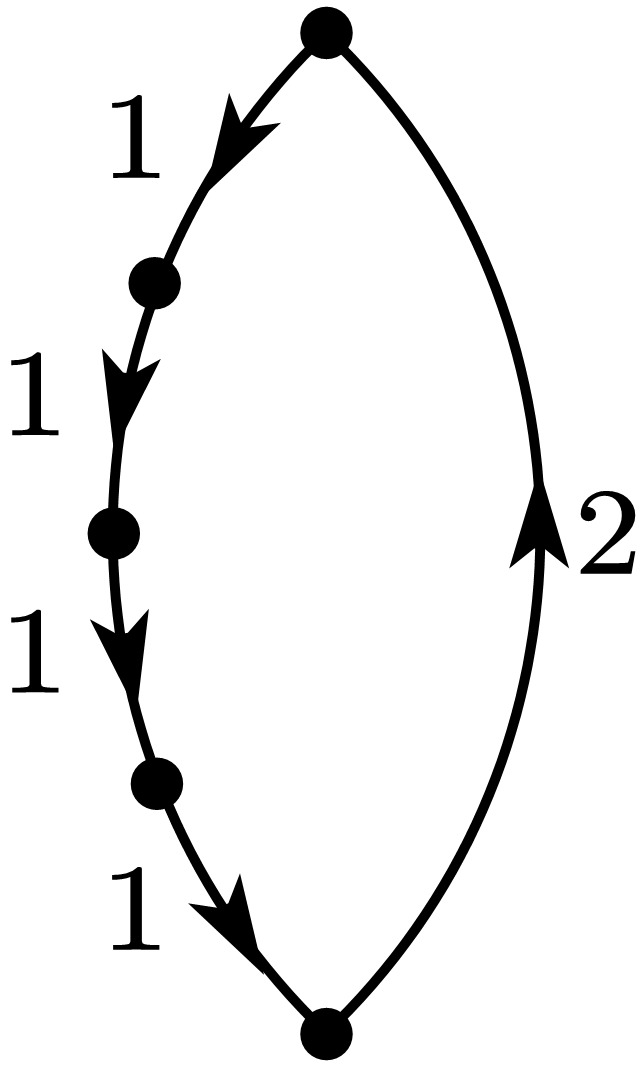
\includegraphics[scale=1.0,trim=0 -4 0 -4]{./pictures/6.01/1.png}
		\captionof*{figure}{$\displaystyle (-1)^{4+1} \frac{ V^3_{11} V_{12} V_{21} }{ ( E^{(0)}_1 - E^{(0)}_2)^4 }$}
		\end{minipage} &
		
		\begin{minipage}{0.22\linewidth}
		\centering
		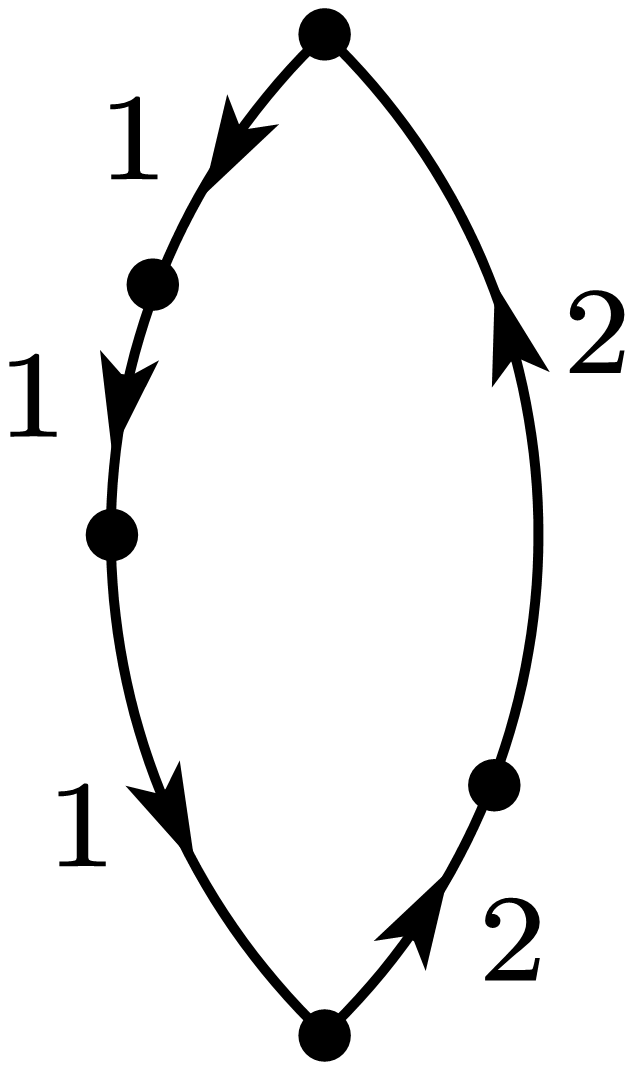
\includegraphics[scale=1.0,trim=0 -4 0 -4]{./pictures/6.01/2.png}
		\captionof*{figure}{$\displaystyle (-1)^{3+1} \frac{ V^2_{11} V_{12} V_{21} V_{22} }{ ( E^{(0)}_1 - E^{(0)}_2)^4 }$}
		\end{minipage} &
		
		\begin{minipage}{0.22\linewidth}
		\centering
		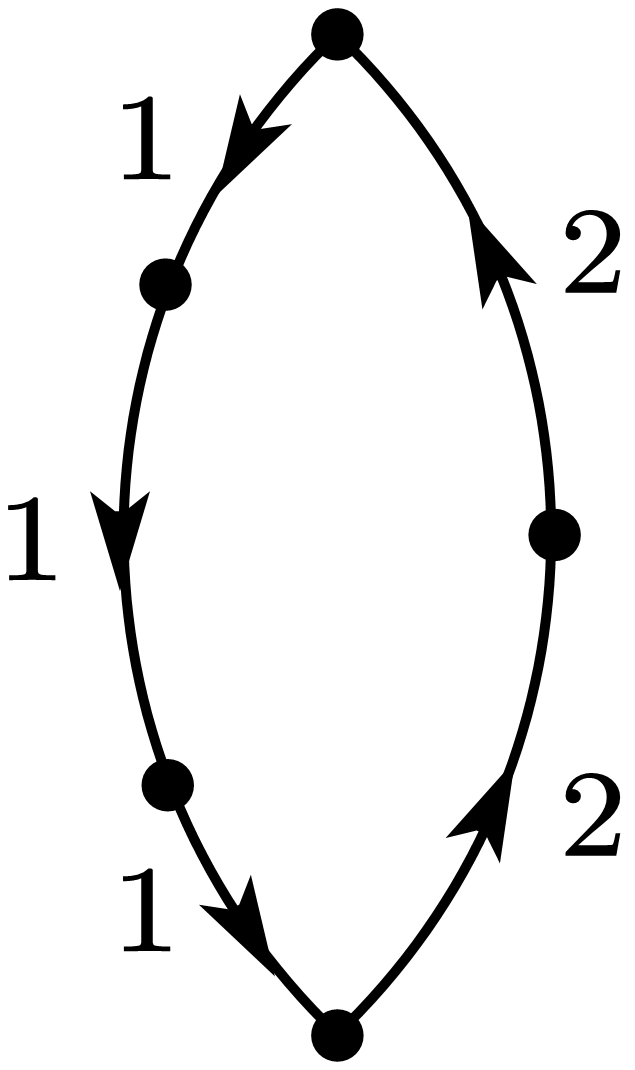
\includegraphics[scale=1.0,trim=0 -4 0 -4]{./pictures/6.01/3.png}
		\captionof*{figure}{$\displaystyle (-1)^{3+1} \frac{ V^2_{11} V_{12} V_{21} V_{22} }{ ( E^{(0)}_1 - E^{(0)}_2)^4 }$}
		\end{minipage} &
		
		\begin{minipage}{0.22\linewidth}
		\centering
		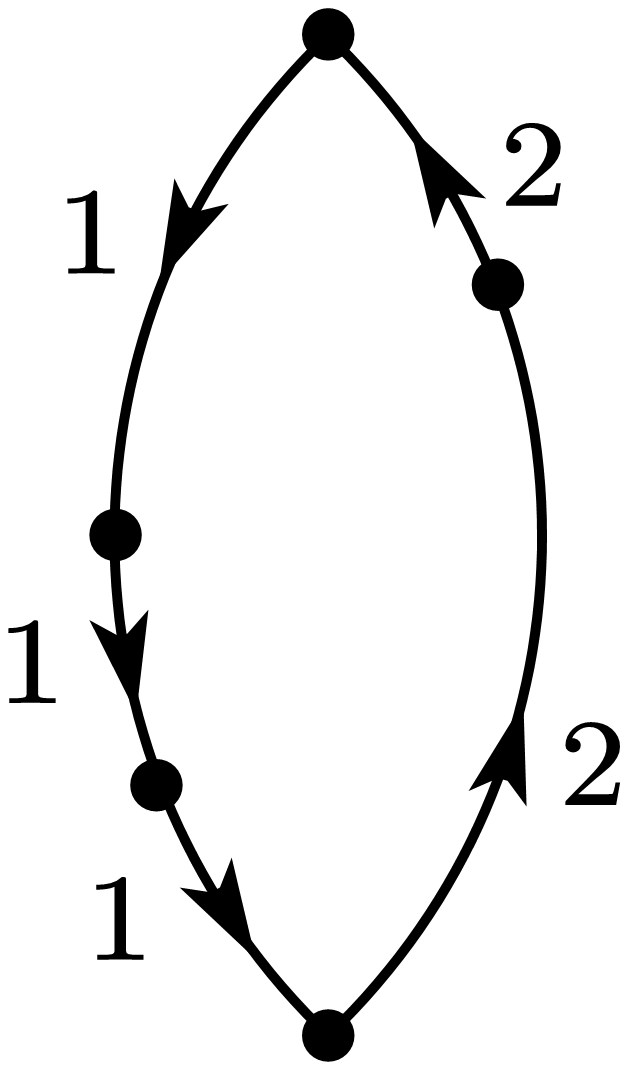
\includegraphics[scale=1.0,trim=0 -4 0 -4]{./pictures/6.01/4.png}
		\captionof*{figure}{$\displaystyle (-1)^{3+1} \frac{ V^2_{11} V_{12} V_{21} V_{22} }{ ( E^{(0)}_1 - E^{(0)}_2)^4 }$}
		\end{minipage} \\
			
		\begin{minipage}{0.22\linewidth}
		\centering
		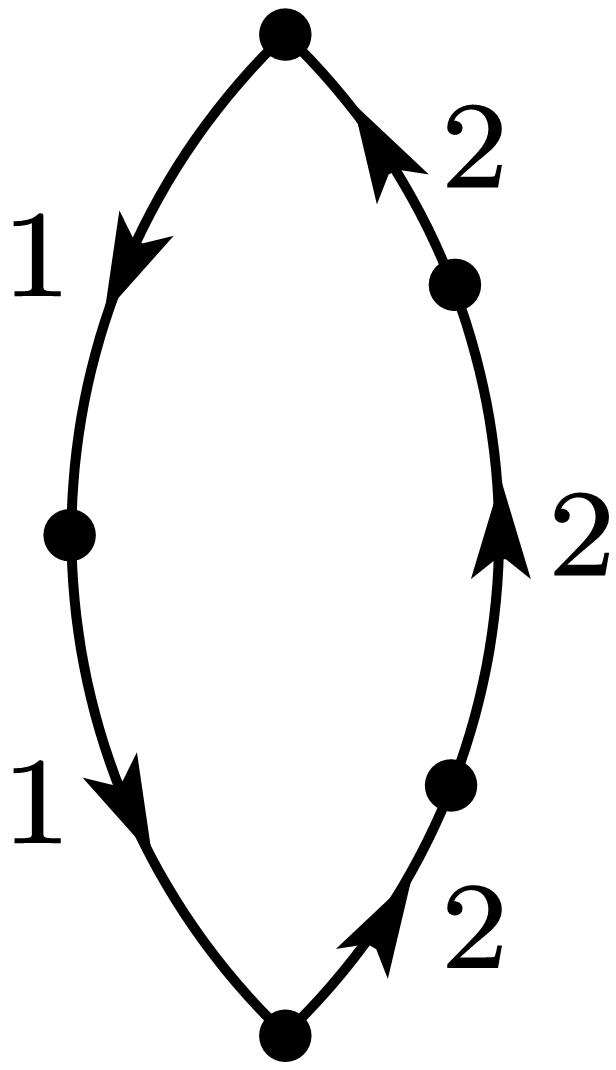
\includegraphics[scale=1.0,trim=0 -4 0 -4]{./pictures/6.01/5.png}
		\captionof*{figure}{$\displaystyle (-1)^{2+1} \frac{ V_{11} V_{12} V_{21} V^2_{22} }{ ( E^{(0)}_1 - E^{(0)}_2)^4 }$}
		\end{minipage} &
		
		\begin{minipage}{0.22\linewidth}
		\centering
		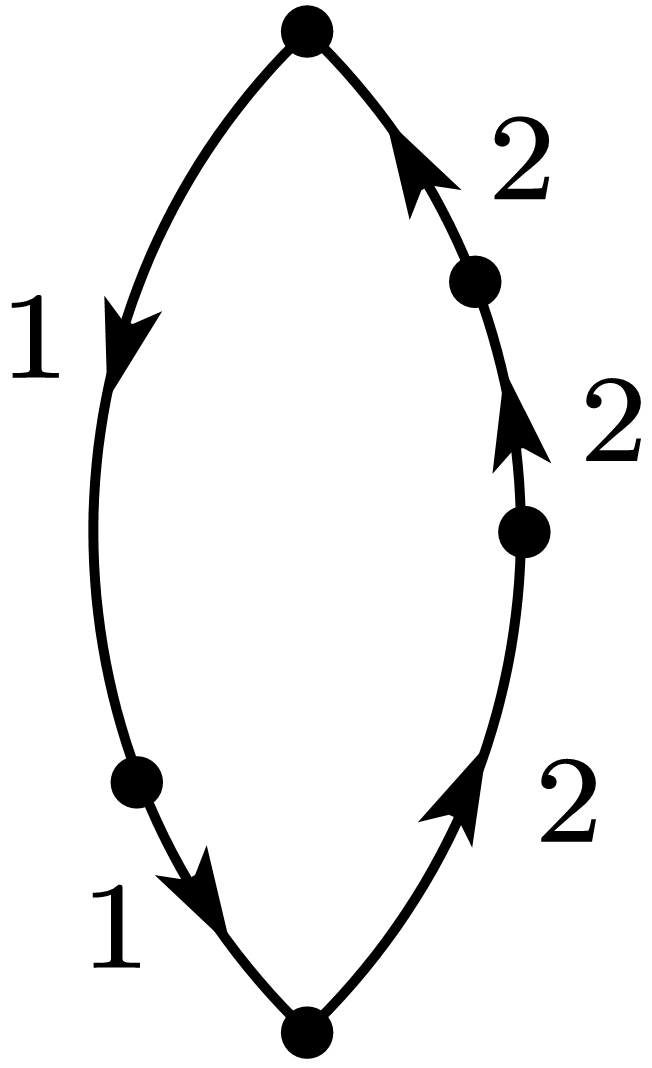
\includegraphics[scale=1.0,trim=0 -4 0 -4]{./pictures/6.01/6.png}
		\captionof*{figure}{$\displaystyle (-1)^{2+1} \frac{ V_{11} V_{12} V_{21} V^2_{22} }{ ( E^{(0)}_1 - E^{(0)}_2)^4 }$}
		\end{minipage} &
		
		\begin{minipage}{0.22\linewidth}
		\centering
		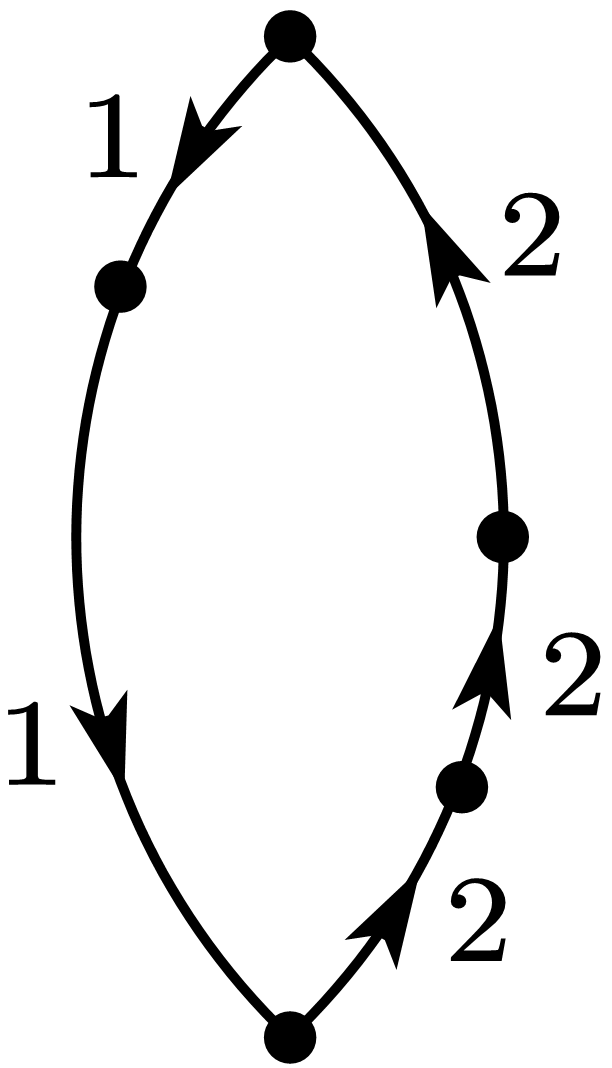
\includegraphics[scale=1.0,trim=0 -4 0 -4]{./pictures/6.01/7.png}
		\captionof*{figure}{$\displaystyle (-1)^{2+1} \frac{ V_{11} V_{12} V_{21} V^2_{22} }{ ( E^{(0)}_1 - E^{(0)}_2)^4 }$}
		\end{minipage} &
		
		\begin{minipage}{0.22\linewidth}
		\centering
		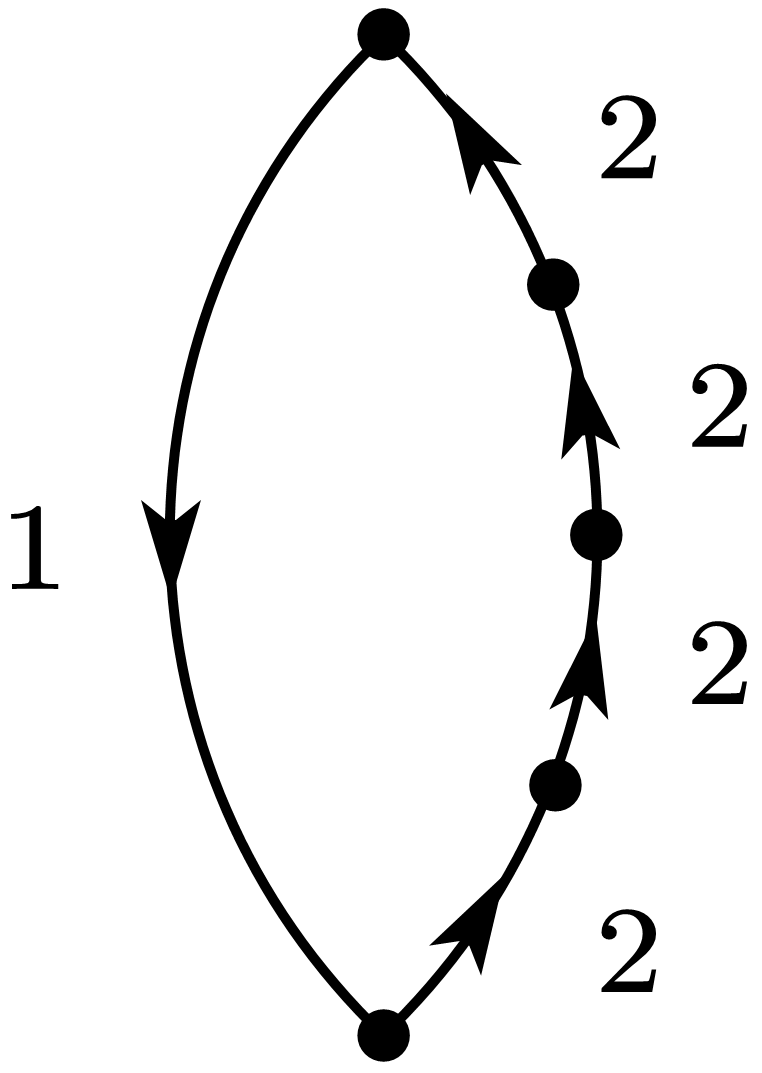
\includegraphics[scale=1.0,trim=0 -4 0 -4]{./pictures/6.01/8.png}
		\captionof*{figure}{$\displaystyle (-1)^{1+1} \frac{ V_{12} V_{21} V^3_{22} }{ ( E^{(0)}_1 - E^{(0)}_2)^4 }$}
		\end{minipage} 
		
	\end{tabular}
	\captionof{figure}{All fifth-order diagrams, which have the property that an imaginary horizontal line crosses only one hole and one particle line, and their mathematical expressions.}\label{fig:exe1}
	\end{center}
	
	Note that the diagrams, which have the property that an imaginary horizontal line crosses only one hole and one particle line, have no pair of hole/particle lines whose overlap is nonempty. For any pair of hole/particle lines which connect the dots $m_1$ and $n_1$, $m_2$ and $n_2$, where $n_1 > m_1$ and $n_2 > m_2$, their overlap will be 
	\begin{itemize}
	
	\item $[\max\{m_1, m_2\},\min\{n_1, n_2\}]$, if $\min\{n_1, n_2\} > \max\{m_1, m_2\}$;
	
	\item empty, otherwise. 
	
	\end{itemize}
	For example, if there is a pair of hole lines, one connecting the dot 1 and 3, and the other connecting 2 and 5, their overlap will be $[2, 3]$. Take an another example, if there is a pair of particle lines, one connecting the dot 5 and 4, and the other connecting 2 and 1, their overlap will be empty.
	
	Thus, there are four cases.
	\begin{itemize}
	
	\item Four hole lines and one particle line. There is only one method, hole lines are $(1,2)$, $(2,3)$, $(3,4)$, $(4,5)$ and the only particle line is $(5,1)$, as the first subdiagram in \Figref{fig:exe1}.
	
	\item Three hole lines and two particle lines. There are three methods as follows.
		\begin{itemize}
	
		\item Hole lines are $(1,2)$, $(2,3)$, and $(3,5)$ while particle lines are $(5,4)$, $(4,1)$.
		
		\item Hole lines are $(1,2)$, $(2,4)$, and $(4,5)$ while particle lines are $(5,3)$, $(3,1)$.
		
		\item Hole lines are $(1,3)$, $(3,4)$, and $(4,5)$ while particle lines are $(5,2)$, $(2,1)$.
	
		\end{itemize}
		They correspond to the second, third, fourth subdiagram in \Figref{fig:exe1}.
	
	\item Two hole lines and three particle lines. There are three methods as follows.
		\begin{itemize}
	
		\item Hole lines are $(1,3)$, $(3,5)$ while particle lines are $(5,4)$, $(4,2)$, and $(2,1)$.
		
		\item Hole lines are $(1,4)$, $(4,5)$ while particle lines are $(5,3)$, $(3,2)$, and $(2,1)$.
		
		\item Hole lines are $(1,2)$, $(2,5)$ while particle lines are $(5,4)$, $(4,3)$, and $(3,1)$.
	
		\end{itemize}
		They correspond to the fifth, sixth, seventh subdiagram in \Figref{fig:exe1}.
		
	\item One hole line and four particle lines. There is only one method, the only hole line is $(1,5)$ and particle lines are $(5,4)$, $(4,3)$, $(3,2)$, and $(2,1)$, as the eighth subdiagram in \Figref{fig:exe1}.
			
	\end{itemize}
	
	Thus, the sum of such diagrams is
	\begin{align*}
%		&\hspace{1.4em}(-1)^{4+1} \frac{ V^3_{11} V_{12} V_{21} }{ ( E^{(0)}_1 - E^{(0)}_2)^4 } + (-1)^{3+1} \frac{ V^2_{11} V_{12} V_{21} V_{22} }{ ( E^{(0)}_1 - E^{(0)}_2)^4 } + (-1)^{3+1} \frac{ V^2_{11} V_{12} V_{21} V_{22} }{ ( E^{(0)}_1 - E^{(0)}_2)^4 } \\
%		&\hspace{1.4em} + (-1)^{3+1} \frac{ V^2_{11} V_{12} V_{21} V_{22} }{ ( E^{(0)}_1 - E^{(0)}_2)^4 } + (-1)^{2+1} \frac{ V_{11} V_{12} V_{21} V^2_{22} }{ ( E^{(0)}_1 - E^{(0)}_2) }^4 + (-1)^{2+1} \frac{ V_{11} V_{12} V_{21} V^2_{22} }{ ( E^{(0)}_1 - E^{(0)}_2) }^4 \\
%		&\hspace{1.4em}  + (-1)^{2+1} \frac{ V_{11} V_{12} V_{21} V^2_{22} }{ ( E^{(0)}_1 - E^{(0)}_2) }^4 + (-1)^{1+1} \frac{ V_{12} V_{21} V^3_{22} }{ ( E^{(0)}_1 - E^{(0)}_2)^4 } \\
%		&= - \frac{ V^3_{11} V_{12} V_{21} }{ ( E^{(0)}_1 - E^{(0)}_2)^4 } + 3 \frac{ V^2_{11} V_{12} V_{21} V_{22} }{ ( E^{(0)}_1 - E^{(0)}_2)^4 } - 3 \frac{ V_{11} V_{12} V_{21} V^2_{22} }{ ( E^{(0)}_1 - E^{(0)}_2) }^4 + \frac{ V_{12} V_{21} V^3_{22} }{ ( E^{(0)}_1 - E^{(0)}_2)^4 } \\
%		&= 
		- \frac{ V_{12} V_{21} \left( V^3_{11} - 3 V^2_{11} V_{22} + 3 V_{11} V_{22} - V^3_{22} \right) }{ ( E^{(0)}_1 - E^{(0)}_2)^4 } = - \frac{ V_{12} V_{21} \left( V_{11} - V_{22} \right)^3 }{ ( E^{(0)}_1 - E^{(0)}_2)^4 } = \frac{ V_{12} V_{21} \left( V_{22} - V_{11} \right)^3 }{ ( E^{(0)}_1 - E^{(0)}_2)^4 }.
	\end{align*}
	
	In fact, as the textbook says, these eight diagrams can be generated by adding three dots to the second-order diagram in all positive ways. In fact, any pair of hole/particle lines in them has also empty overlap. I think the calculation of the overlap is much direct than inspecting the property of lines.
	
	\end{solution}

	\subsection{Diagrammatic Perturbation Theory for \texorpdfstring{$N$}- States}
	
	% 6.2
	\begin{exercise}
	Use diagrammatic techniques to obtain the fourth-order perturbation energy of a particular state (say, $i$) of an $N$-state system. That is, evaluate the diagrams
	\begin{center}
	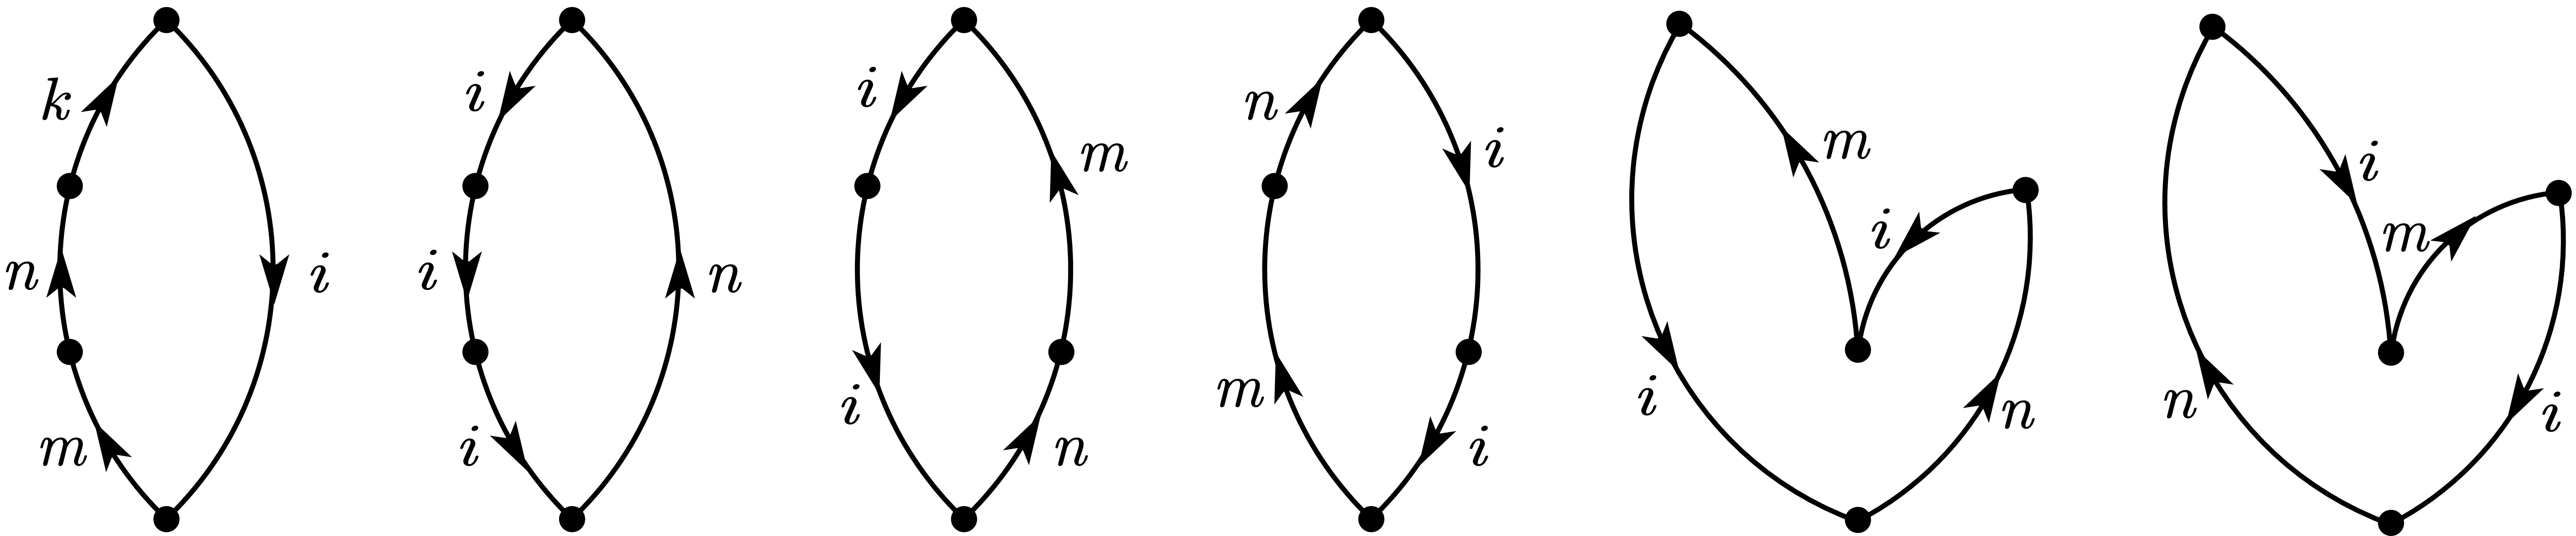
\includegraphics[scale=1.0]{./pictures/6.02/exercise.png}
	\end{center}
	where the indices $m$, $n$, $k$, ... exclude $i$. Using the approach of Section 6.1, obtain an algebraic expression for the fourth-order energy and compare it to the diagrammatic result.
	
	\end{exercise}
	
	\begin{solution}
	
	Firstly, all fourth-order diagrams and their mathematical expressions are listed in \Figref{fig:exe2}.
	
	\begin{center}
	\begin{tabular}{cc}
	
		\begin{minipage}{0.49\linewidth}
		\centering
		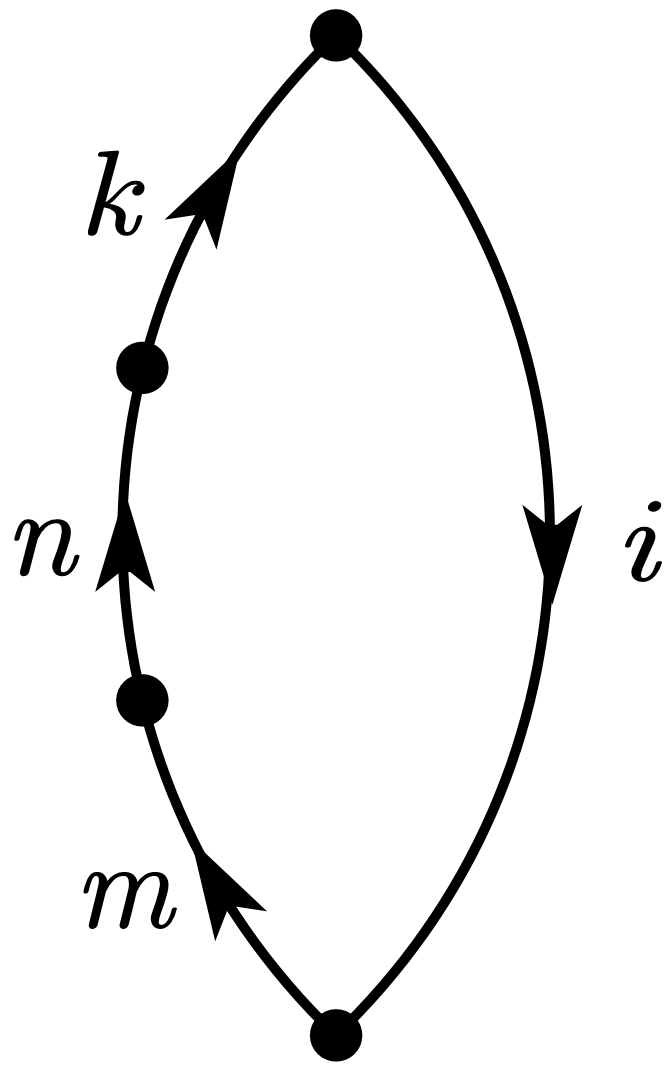
\includegraphics[scale=1.0,trim=0 -4 0 -4]{./pictures/6.02/1.png}
		\captionof*{figure}{$(-1)^{1+1} { \sum_{kmn} }^\prime \frac{ V_{ki} V_{nk} V_{mn} V_{im} }{ ( E^{(0)}_i - E^{(0)}_k ) ( E^{(0)}_i - E^{(0)}_n ) ( E^{(0)}_i - E^{(0)}_m ) }$}
		\end{minipage} &
		
		\begin{minipage}{0.42\linewidth}
		\centering
		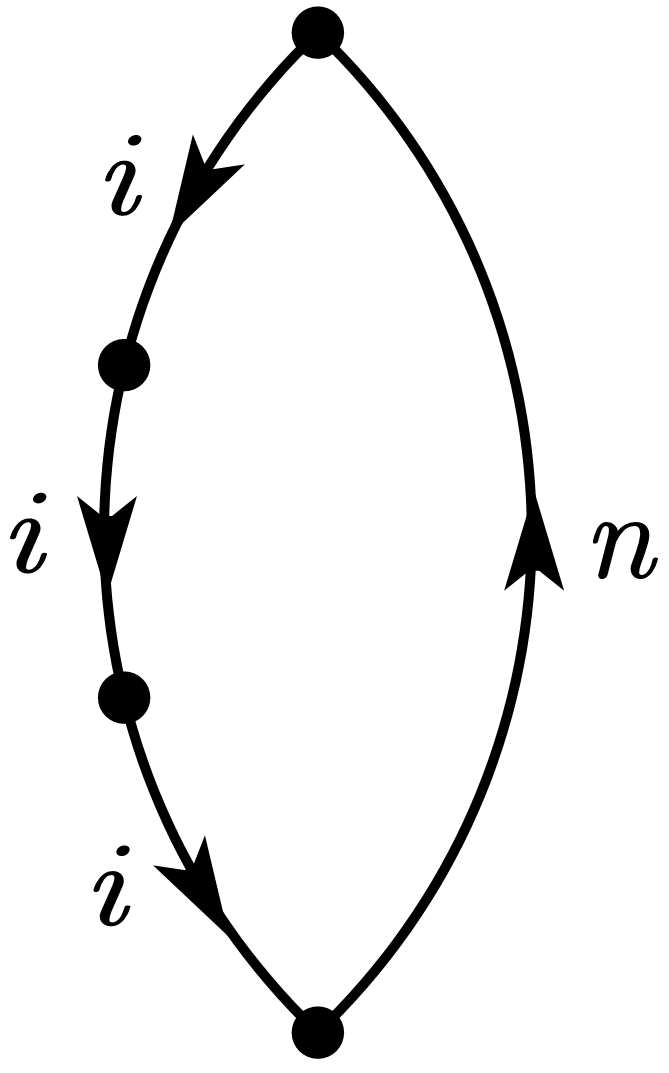
\includegraphics[scale=1.0,trim=0 -4 0 -4]{./pictures/6.02/2.png}
		\captionof*{figure}{$(-1)^{3+1} { \sum_n }^\prime \frac{ V_{ni} V^2_{ii} V_{in} }{ ( E^{(0)}_i - E^{(0)}_n)^3 }$}
		\end{minipage} \\
		
		\begin{minipage}{0.49\linewidth}
		\centering
		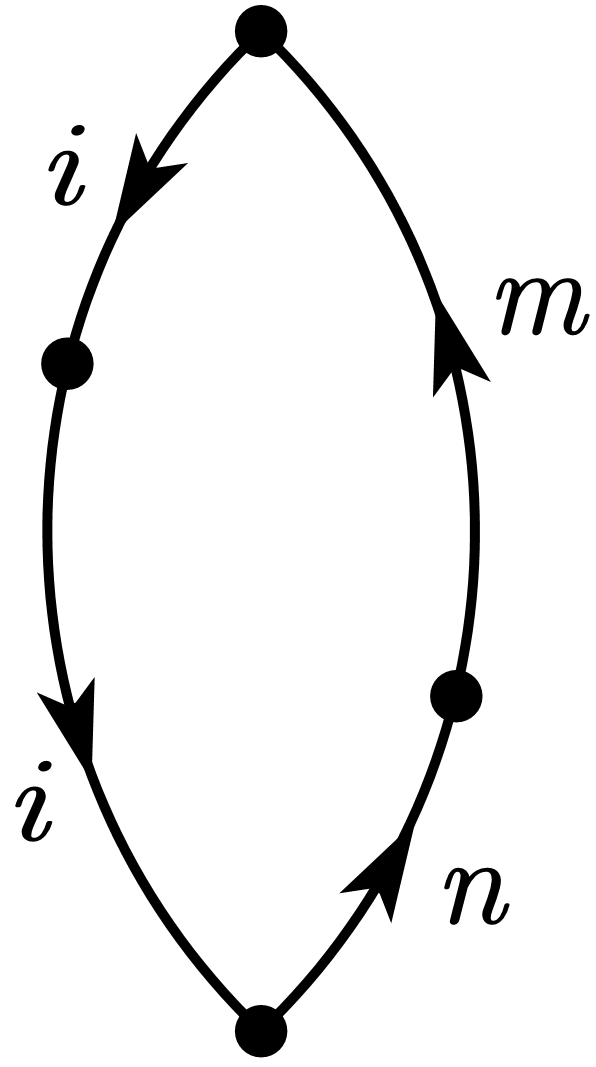
\includegraphics[scale=1.0,trim=0 -4 0 -4]{./pictures/6.02/3.png}
		\captionof*{figure}{$(-1)^{2+1} { \sum_{mn} }^\prime \frac{ V_{mi} V_{ii} V_{in} V_{nm} }{ ( E^{(0)}_i - E^{(0)}_n) ( E^{(0)}_i - E^{(0)}_m )^2 }$}
		\end{minipage}  &
			
		\begin{minipage}{0.42\linewidth}
		\centering
		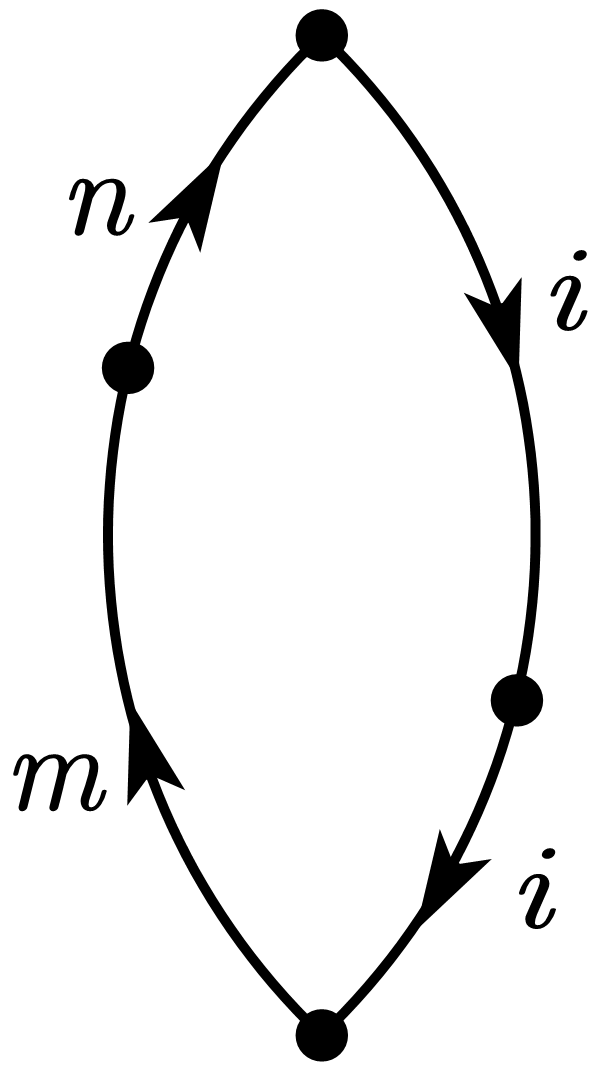
\includegraphics[scale=1.0,trim=0 -4 0 -4]{./pictures/6.02/4.png}
		\captionof*{figure}{$(-1)^{2+1} { \sum_{mn} }^\prime \frac{ V_{ni} V_{ii} V_{im} V_{mn} }{ ( E^{(0)}_i - E^{(0)}_n) ( E^{(0)}_i - E^{(0)}_m )^2 }$}
		\end{minipage} \\
		
		\begin{minipage}{0.49\linewidth}
		\centering
		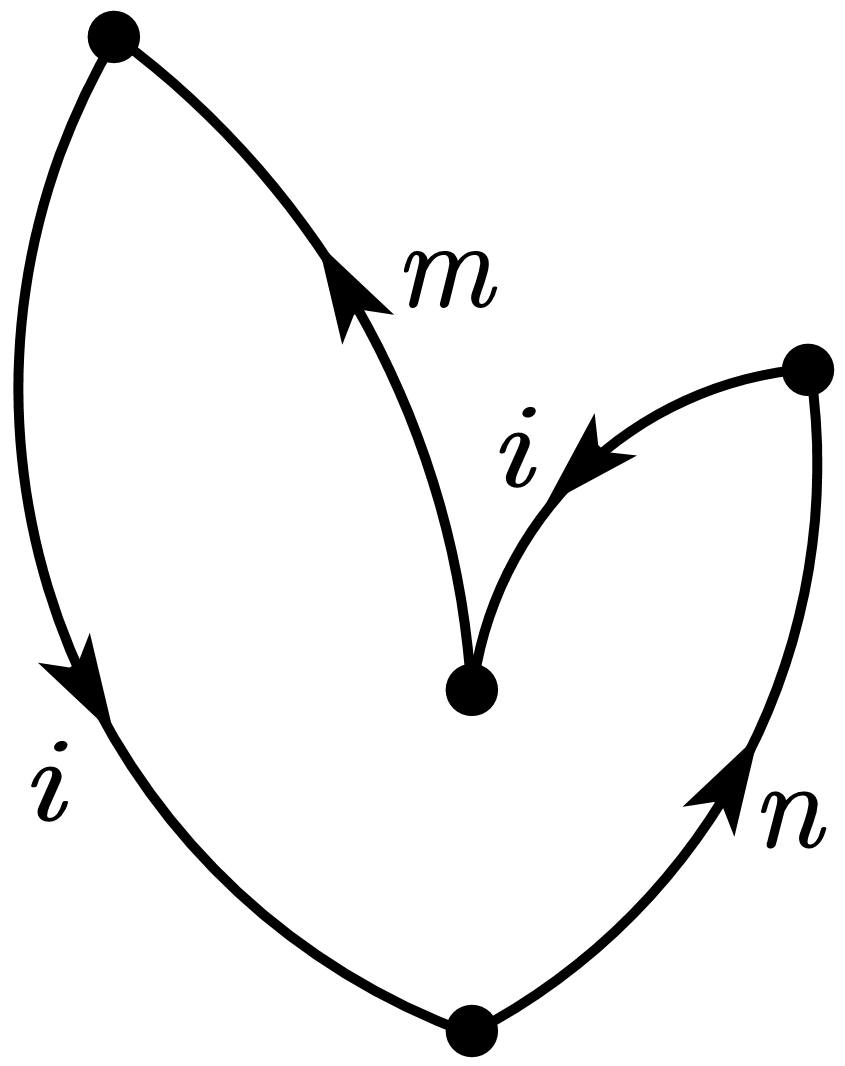
\includegraphics[scale=1.0,trim=0 -4 0 -4]{./pictures/6.02/5.png}
		\captionof*{figure}{$(-1)^{2+1} { \sum_{mn} }^\prime \frac{ V_{mi} V_{in} V_{ni} V_{im} }{ ( E^{(0)}_i - E^{(0)}_m ) ( 2E^{(0)}_i - E^{(0)}_m - E^{(0)}_n ) ( E^{(0)}_i - E^{(0)}_n ) }$}
		\end{minipage} &
		
		\begin{minipage}{0.42\linewidth}
		\centering
		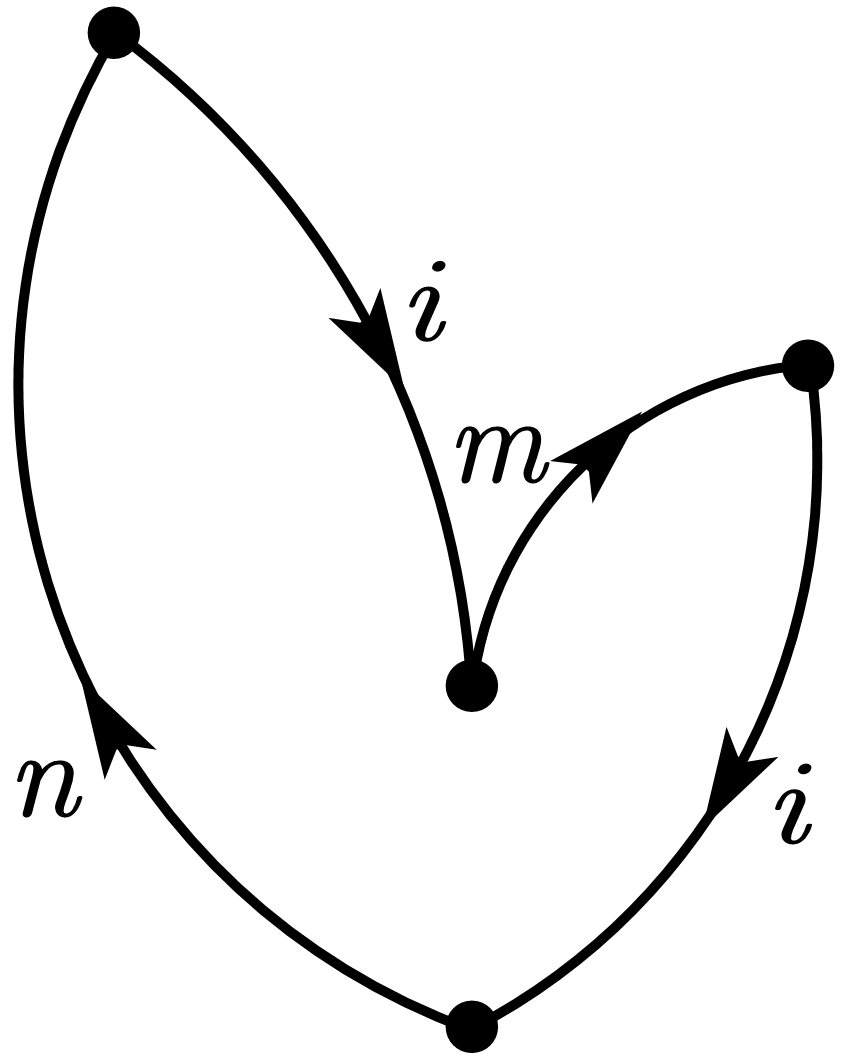
\includegraphics[scale=1.0,trim=0 -4 0 -4]{./pictures/6.02/6.png}
		\captionof*{figure}{$(-1)^{2+1} { \sum_{mn} }^\prime \frac{ V_{in} V_{ni} V_{im} V_{mi} }{ ( 2E^{(0)}_i - E^{(0)}_m - E^{(0)}_n ) ( E^{(0)}_i - E^{(0)}_n )^2 }$}
		\end{minipage} 
				
	\end{tabular}
	\captionof{figure}{All fourth-order diagrams and their mathematical expressions.}\label{fig:exe2}
	\end{center}
	
	Before the formal algebraic derivation, we should obtain some useful intermediate results. From (6.7d), multiplying by $\langle n |$, where $n \neq i$, we find that
	\[
		E^{(0)}_n \langle n | \Psi^{(3)}_i \rangle + \langle n | \mathscr{V} | \Psi^{(2)}_i \rangle = E^{(0)}_i \langle n | \Psi^{(3)}_i \rangle + E^{(1)}_i \langle n | \Psi^{(2)}_i \rangle + E^{(1)}_i \langle n | \Psi^{(2)}_i \rangle,
	\]
	and thus
	\[
		\langle n | \Psi^{(3)}_i \rangle = \frac{ 1 }{ E^{(0)}_i - E^{(0)}_n }\left[ \langle n | \mathscr{V} | \Psi^{(2)}_i \rangle - E^{(1)}_i \langle n | \Psi^{(2)}_i \rangle - E^{(1)}_i \langle n | \Psi^{(2)}_i \rangle \right].
	\]
	Moreover, (6.8b), (6.10), (6.12), and (6.14) are used in the formal derivation. The fourth-order perturbation energy $E^{(4)}_i$ can be divided into 3 terms, viz.,
	\begin{align*}
		E^{(4)}_i &= \langle i | \mathscr{V} | \Psi^{(3)}_i \rangle = { \sum_n }^\prime \langle i | \mathscr{V} | n \rangle \langle n | \Psi^{(3)}_i \rangle = { \sum_n }^\prime V_{in} \frac{ \langle n | \mathscr{V} | \Psi^{(2)}_i \rangle - E^{(1)}_i \langle n | \Psi^{(2)}_i \rangle - E^{(2)}_i \langle n | \Psi^{(1)}_i \rangle }{ E^{(0)}_i - E^{(0)}_n } \\
		&= { \sum_n }^\prime \frac{ V_{in} \langle n | \mathscr{V} | \Psi^{(2)}_i \rangle }{ E^{(0)}_i - E^{(0)}_n } - E^{(1)}_i { \sum_n }^\prime \frac{ V_{in} \langle n | \Psi^{(2)}_i \rangle }{ E^{(0)}_i - E^{(0)}_n } - E^{(2)}_i { \sum_n }^\prime \frac{ V_{in} \langle n | \Psi^{(1)}_i \rangle }{ E^{(0)}_i - E^{(0)}_n }.
	\end{align*}		
	The first term is
	\begin{align*}
		&\hspace{1.4em}{ \sum_n }^\prime \frac{ V_{in} \langle n | \mathscr{V} | \Psi^{(2)}_i \rangle }{ E^{(0)}_i - E^{(0)}_n } = { \sum_{mn} }^\prime \frac{ V_{in} \langle n | \mathscr{V} | m \rangle \langle m | \Psi^{(2)}_i \rangle }{ E^{(0)}_i - E^{(0)}_n } = { \sum_{mn} }^\prime \frac{ V_{in} V_{nm} }{ E^{(0)}_i - E^{(0)}_n } \langle m | \Psi^{(2)}_i \rangle \\
		&= { \sum_{mn} }^\prime \frac{ V_{in} V_{nm} }{ E^{(0)}_i - E^{(0)}_n } \frac{ \langle m | \mathscr{V} | \Psi^{(1)}_i \rangle - E^{(1)}_i \langle m | \Psi^{(1)}_i \rangle }{ E^{(0)}_i - E^{(0)}_m } \\
		&= { \sum_{mn} }^\prime \frac{ V_{in} V_{nm} }{ ( E^{(0)}_i - E^{(0)}_n )( E^{(0)}_i - E^{(0)}_m ) } \left[ \langle m | \mathscr{V} | \Psi^{(1)}_i \rangle - E^{(1)}_i \langle m | \Psi^{(1)}_i \rangle \right] \\
		&= { \sum_{mn} }^\prime \frac{ V_{in} V_{nm} }{ (E^{(0)}_i - E^{(0)}_n) (E^{(0)}_i - E^{(0)}_m) } \left[ { \sum_k }^\prime \langle m | \mathscr{V} | k \rangle \langle k | \Psi^{(1)}_i \rangle - E^{(1)}_i \langle m | \Psi^{(1)}_i \rangle \right] \\
		&= { \sum_{mnk} }^\prime \frac{ V_{in} V_{nm} V_{mk} }{ (E^{(0)}_i - E^{(0)}_n) (E^{(0)}_i - E^{(0)}_m) } \langle k | \Psi^{(1)}_i \rangle - { \sum_{mn} }^\prime \frac{ V_{ii} V_{in} V_{nm} }{ (E^{(0)}_i - E^{(0)}_n) (E^{(0)}_i - E^{(0)}_m) } \langle m | \Psi^{(1)}_i \rangle \\
		&= { \sum_{mnk} }^\prime \frac{ V_{in} V_{nm} V_{mk} }{ (E^{(0)}_i - E^{(0)}_n) (E^{(0)}_i - E^{(0)}_m) } \frac{ V_{ki} }{ E^{(0)}_i - E^{(0)}_k } - { \sum_{mn} }^\prime \frac{ V_{ii} V_{in} V_{nm} }{ (E^{(0)}_i - E^{(0)}_n) (E^{(0)}_i - E^{(0)}_m) } \frac{ V_{mi} }{ E^{(0)}_i - E^{(0)}_m } \\
		&= { \sum_{mnk} }^\prime \frac{ V_{in} V_{nm} V_{mk} V_{ki} }{ (E^{(0)}_i - E^{(0)}_n) (E^{(0)}_i - E^{(0)}_m) (E^{(0)}_i - E^{(0)}_k) } - { \sum_{mn} }^\prime \frac{ V_{ii} V_{in} V_{nm} V_{mi} }{ (E^{(0)}_i - E^{(0)}_n) (E^{(0)}_i - E^{(0)}_m)^2 } \\
		&= { \sum_{mnk} }^\prime \frac{ V_{im} V_{mn} V_{nk} V_{ki} }{ (E^{(0)}_i - E^{(0)}_n) (E^{(0)}_i - E^{(0)}_m) (E^{(0)}_i - E^{(0)}_k) } - { \sum_{mn} }^\prime \frac{ V_{ii} V_{in} V_{nm} V_{mi} }{ (E^{(0)}_i - E^{(0)}_n) (E^{(0)}_i - E^{(0)}_m)^2 }.
	\end{align*}
	It is evident that the first part of the first term correspond to the first subdiagram and the second part of the first term correspond to the third subdiagram.
	
	The second term is
	\begin{align*}
		&\hspace{1.4em}- E^{(1)}_i { \sum_n }^\prime \frac{ V_{in} \langle n | \Psi^{(2)}_i \rangle }{ E^{(0)}_i - E^{(0)}_n } - { \sum_n }^\prime \frac{ V_{ii} V_{in} }{ E^{(0)}_i - E^{(0)}_n } \langle n | \Psi^{(2)}_i \rangle \\
		&= - { \sum_n }^\prime \frac{ V_{ii} V_{in} }{ E^{(0)}_i - E^{(0)}_n } \frac{ \langle n | \mathscr{V} | \Psi^{(1)}_i \rangle - E^{(1)}_i \langle n | \Psi^{(1)}_i \rangle }{ E^{(0)}_i - E^{(0)}_n } \\
		&= - { \sum_n }^\prime \frac{ V_{ii} V_{in} }{ ( E^{(0)}_i - E^{(0)}_n )^2 } \langle n | \mathscr{V} | \Psi^{(1)}_i \rangle + E^{(1)}_i { \sum_n }^\prime \frac{ V_{ii} V_{in} }{ ( E^{(0)}_i - E^{(0)}_n )^2 } \langle n | \Psi^{(1)}_i \rangle \\
		&= - { \sum_n }^\prime \frac{ V_{ii} V_{in} }{ ( E^{(0)}_i - E^{(0)}_n )^2 } { \sum_m }^\prime \langle n | \mathscr{V} | m \rangle \langle m | \Psi^{(1)}_i \rangle + { \sum_n }^\prime \frac{ V^2_{ii} V_{in} }{ ( E^{(0)}_i - E^{(0)}_n )^2 } \langle n | \Psi^{(1)}_i \rangle \\
		&= - { \sum_{mn} }^\prime \frac{ V_{ii} V_{in} V_{nm} }{ ( E^{(0)}_i - E^{(0)}_n )^2 } \langle m | \Psi^{(1)}_i \rangle + { \sum_n }^\prime \frac{ V^2_{ii} V_{in} }{ ( E^{(0)}_i - E^{(0)}_n )^2 } \langle n | \Psi^{(1)}_i \rangle \\
		&= - { \sum_{mn} }^\prime \frac{ V_{ii} V_{in} V_{nm} }{ ( E^{(0)}_i - E^{(0)}_n )^2 } \frac{ \langle m | \mathscr{V} | i \rangle }{ E^{(0)}_i - E^{(0)}_m } + { \sum_n }^\prime \frac{ V^2_{ii} V_{in} }{ ( E^{(0)}_i - E^{(0)}_n )^2 } \frac{ \langle n | \mathscr{V} | i \rangle }{ E^{(0)}_i - E^{(0)}_n } \\
		&= - { \sum_{mn} }^\prime \frac{ V_{ii} V_{in} V_{nm} V_{mi} }{ ( E^{(0)}_i - E^{(0)}_n )^2 (E^{(0)}_i - E^{(0)}_m) } + { \sum_n }^\prime \frac{ V^2_{ii} V_{in} V_{ni} }{ ( E^{(0)}_i - E^{(0)}_n )^3 } \\
		&= - { \sum_{mn} }^\prime \frac{ V_{ii} V_{im} V_{mn} V_{ni} }{ ( E^{(0)}_i - E^{(0)}_m )^2 ( E^{(0)}_i - E^{(0)}_n ) } + { \sum_n }^\prime \frac{ V^2_{ii} V_{in} V_{ni} }{ ( E^{(0)}_i - E^{(0)}_n )^3 } .
	\end{align*}
	It is evident that the first part of the second term correspond to the fourth subdiagram and the second part of the second term correspond to the second subdiagram.
	
	The third term is
	\begin{align*}
		&\hspace{1.4em} -E^{(2)}_i { \sum_n }^\prime \frac{ V_{in} \langle n | \Psi^{(1)}_i \rangle }{ E^{(0)}_i - E^{(0)}_n } = -E^{(2)}_i { \sum_n }^\prime \frac{ V_{in} }{ E^{(0)}_i - E^{(0)}_n } \frac{ \langle n | \mathscr{V} | i \rangle }{ E^{(0)}_i - E^{(0)}_n } = -E^{(2)}_i { \sum_n }^\prime \frac{ V_{in} V_{ni} }{ ( E^{(0)}_i - E^{(0)}_n )^2 } \\
		&= - \left( { \sum_m }^\prime \frac{ V_{im} V_{mi} }{ ( E^{(0)}_i - E^{(0)}_m ) } \right) { \sum_n }^\prime \frac{ V_{in} V_{ni} }{ ( E^{(0)}_i - E^{(0)}_n )^2 } = - { \sum_{mn} }^\prime \frac{ V_{im} V_{mi} V_{in} V_{ni} }{ ( E^{(0)}_i - E^{(0)}_m )( E^{(0)}_i - E^{(0)}_n )^2 } .
	\end{align*}		
	
	It seems that it does not directly correspond to any subdiagram in \Figref{fig:exe2}. However, we can find that the sum of the mathematical expressions of the fifth and sixth subdiagram is
	\begin{align*}
		&\hspace{1.4em}(-1)^{2+1} { \sum_{mn} }^\prime \frac{ V_{mi} V_{in} V_{ni} V_{im} }{ ( E^{(0)}_i - E^{(0)}_m ) ( 2E^{(0)}_i - E^{(0)}_m - E^{(0)}_n ) ( E^{(0)}_i - E^{(0)}_n ) }  \\
		&\hspace{3.4em}+ (-1)^{2+1} { \sum_{mn} }^\prime \frac{ V_{in} V_{ni} V_{im} V_{mi} }{ ( 2E^{(0)}_i - E^{(0)}_m - E^{(0)}_n ) ( E^{(0)}_i - E^{(0)}_n )^2 } \\
		&= - { \sum_{mn} }^\prime \frac{ V_{in} V_{ni} V_{im} V_{mi} }{ ( 2E^{(0)}_i - E^{(0)}_m - E^{(0)}_n ) ( E^{(0)}_i - E^{(0)}_n ) } \left[ \frac{ 1 }{ E^{(0)}_i - E^{(0)}_m } + \frac{ 1 }{ E^{(0)}_i - E^{(0)}_n } \right] \\
		&= - { \sum_{mn} }^\prime \frac{ V_{in} V_{ni} V_{im} V_{mi} }{ ( 2E^{(0)}_i - E^{(0)}_m - E^{(0)}_n ) ( E^{(0)}_i - E^{(0)}_n ) } \frac{ 2E^{(0)}_i - E^{(0)}_m - E^{(0)}_n }{ ( E^{(0)}_i - E^{(0)}_m )( E^{(0)}_i - E^{(0)}_n ) } \\
		&= - { \sum_{mn} }^\prime \frac{ V_{im} V_{mi} V_{in} V_{ni} }{ ( E^{(0)}_i - E^{(0)}_m )( E^{(0)}_i - E^{(0)}_n )^2 } ,
	\end{align*}
	which is the third term exactly. Thus we can conclude that the results obtained by algebraic methods is the same as that by diagrammatic techniques. The mathematical expression of the fourth-order perturbation energy $E^{(4)}_i$ is
	\begin{align*}
		E^{(4)}_i &= { \sum_{mnk} }^\prime \frac{ V_{im} V_{mn} V_{nk} V_{ki} }{ (E^{(0)}_i - E^{(0)}_n) (E^{(0)}_i - E^{(0)}_m) (E^{(0)}_i - E^{(0)}_k) } - { \sum_{mn} }^\prime \frac{ V_{ii} V_{in} V_{nm} V_{mi} }{ (E^{(0)}_i - E^{(0)}_n) (E^{(0)}_i - E^{(0)}_m)^2 } \\
		&\hspace{2em} - { \sum_{mn} }^\prime \frac{ V_{ii} V_{im} V_{mn} V_{ni} }{ ( E^{(0)}_i - E^{(0)}_m )^2 ( E^{(0)}_i - E^{(0)}_n ) } + { \sum_n }^\prime \frac{ V^2_{ii} V_{in} V_{ni} }{ ( E^{(0)}_i - E^{(0)}_n )^3 } - { \sum_{mn} }^\prime \frac{ V_{im} V_{mi} V_{in} V_{ni} }{ ( E^{(0)}_i - E^{(0)}_m )( E^{(0)}_i - E^{(0)}_n )^2 } .
	\end{align*}
	
	\end{solution}
	
	\subsection{Summation of Diagrams}
	
	\section{Orbital Perturbation Theory: One-Particle Perturbations}	
	
	% 6.3	
	\begin{exercise}
	Derive
	\[
		E^{(2)}_0 = \sum_{ar} \frac{v_{ar}v_{ra}}{\varepsilon^{(0)}_a - \varepsilon^{(0)}_r}
	\]
	starting with the general expression for the second-order energy (Eq.(6.12)) applied to an $N$-electron system,
	\[
		E^{(2)}_0 = { \sum_n }^\prime \frac{\left| \langle \Psi_0 | \displaystyle\sum_i v(i)| n \rangle \right|^2 }{E^{(0)}_0-E^{(0)}_n}
	\]
	where the sum runs over all states of the system except the ground state.
	
	{\it Hint}: The states $| n \rangle$ must be single excitations of the type
	\[
		|\Psi^r_a\rangle = | \chi^{(0)}_1 \cdots \chi^{(0)}_{a-1} \chi^{(0)}_{r} \chi^{(0)}_{a+1} \cdots \chi^{(0)}_{N} \rangle.
	\]
	\end{exercise}
	
	\begin{solution}
	
	Note that (6.31) states that $\mathscr{V}=\sum_i v(i)$ only connects two Slater determinants whose different occupied orbitals should be no more than one, thus we obtain that
	\begin{sequation}
		E^{(2)}_0 = { \sum_n }^\prime \frac{\left| \langle \Psi_0 | \sum_i v(i)| n \rangle \right|^2 }{E^{(0)}_0-E^{(0)}_n} = \sum_{ ar } \frac{ \left| \langle \Psi_0 | \mathscr{V} | \Psi^r_a \rangle \right|^2 }{E^{(0)}_0-(E^{(0)}_0 + \varepsilon^{(0)}_r - \varepsilon^{(0)}_a) } = \sum_{ ar } \frac{ v_{ar} v_{ra} }{ \varepsilon^{(0)}_a - \varepsilon^{(0)}_r }.
	\end{sequation}
	
	\end{solution}
	
	% 6.4
	\begin{exercise}
	Calculate the third-order energy $E^{(3)}_0$ using the general expression given in Eq.(6.15).
	\begin{enumerate}
	
	\item[a.] Show that
	\[
		B^{(3)}_0 = - E^{(1)}_0 { \sum_n }^\prime \frac{|\langle \Psi_0 | \mathscr{V} | n \rangle |^2}{(E^{(0)}_0-E^{(0)}_n)^2} = - \sum_{abr} \frac{v_{aa} v_{rb} v_{br}}{( \varepsilon^{(0)}_b - \varepsilon^{(0)}_r)^2}.
	\]
		
	\item[b.] Show that
	\[
		A^{(3)}_0 = { \sum_{nm} }^\prime \frac{\langle \Psi_0 | \mathscr{V} | n \rangle \langle n | \mathscr{V} | m \rangle \langle m | \mathscr{V} | \Psi_0 \rangle}{(E^{(0)}_0-E^{(0)}_n)(E^{(0)}_0-E^{(0)}_m)} = \sum_{abrs} \frac{v_{ar} v_{sb} \langle \Psi^r_a | \mathscr{V} | \Psi^s_b \rangle}{( \varepsilon^{(0)}_a - \varepsilon^{(0)}_r)( \varepsilon^{(0)}_b - \varepsilon^{(0)}_s)}.
	\]
	
	\item[c.] Show that
	\begin{align*}
		\langle \Psi^r_a | \mathscr{V} | \Psi^s_b \rangle &= v_{rs} & \text{if} \, a = b  \quad r \neq s, \\
		&= - v_{ba} & \text{if} \, a \neq b \quad r = s, \\
		&= \sum_{c} v_{cc} - v_{aa} + v_{rr} & \text{if} \, a = b \quad r = s ,
	\end{align*}
	and zero otherwise.
		
	\item[d.] Finally, combine the two terms to obtain
	\[
		E^{(3)}_0 = A^{(3)}_0 + B^{(3)}_0 = \sum_{ars} \frac{v_{ar} v_{rs} v_{sa}}{( \varepsilon^{(0)}_a - \varepsilon^{(0)}_r)( \varepsilon^{(0)}_a - \varepsilon^{(0)}_s)} - \sum_{abr} \frac{v_{ra} v_{ab} v_{br}}{( \varepsilon^{(0)}_a - \varepsilon^{(0)}_r) ( \varepsilon^{(0)}_b - \varepsilon^{(0)}_r)}.
	\]
	
	\item[e.] Show that for a chosed-shell system
	\[
		E^{(3)}_0 = 2\sum_{ars}^{N/2} \frac{v_{ar} v_{rs} v_{sa}}{( \varepsilon^{(0)}_a - \varepsilon^{(0)}_r)( \varepsilon^{(0)}_a - \varepsilon^{(0)}_s)} - 2\sum_{abr}^{N/2} \frac{v_{ra} v_{ab} v_{br}}{( \varepsilon^{(0)}_a - \varepsilon^{(0)}_r) ( \varepsilon^{(0)}_b - \varepsilon^{(0)}_r)}.
	\]
	
	\end{enumerate}
	\end{exercise}
	
	\begin{solution}
	
	\begin{itemize}
	
	\item[a.] Similar to Exercise 6.3, it is evident that
	\begin{align*}
		B^{(3)}_0 &= - E^{(1)}_0 { \sum_n }^\prime \frac{|\langle \Psi_0 | \mathscr{V} | n \rangle |^2}{(E^{(0)}_0-E^{(0)}_n)^2} = - \left( \sum_{a} v_{aa} \right) \sum_{br} \frac{ v_{rb} v_{br}}{[ E^{(0)}_0- ( E^{(0)}_n + \varepsilon^{(0)}_r - \varepsilon^{(0)}_b ) ]^2} \\
		&= - \sum_{abr} \frac{ v_{aa} v_{rb} v_{br}}{( \varepsilon^{(0)}_b - \varepsilon^{(0)}_r)^2}.
	\end{align*}

	\item[b.] In the same way, we obtain that
	\begin{align*}
		A^{(3)}_0 &= { \sum_{nm} }^\prime \frac{\langle \Psi_0 | \mathscr{V} | n \rangle \langle n | \mathscr{V} | m \rangle \langle m | \mathscr{V} | \Psi_0 \rangle}{(E^{(0)}_0-E^{(0)}_n)(E^{(0)}_0-E^{(0)}_m)} \\
		&= \sum_{ar} \sum_{bs} \frac{\langle \Psi_0 | \mathscr{V} | \Psi^r_a \rangle \langle \Psi^r_a | \mathscr{V} | \Psi^s_b \rangle \langle \Psi^s_b | \mathscr{V} | \Psi_0 \rangle}{ [ E^{(0)}_0 - ( E^{(0)}_0 + \varepsilon^{(0)}_r - \varepsilon^{(0)}_a ) ][ E^{(0)}_0 - ( E^{(0)}_0 + \varepsilon^{(0)}_s - \varepsilon^{(0)}_b ) ]}  \\
		&= \sum_{abrs} \frac{v_{ar} v_{sb} \langle \Psi^r_a | \mathscr{V} | \Psi^s_b \rangle}{( \varepsilon^{(0)}_a - \varepsilon^{(0)}_r)( \varepsilon^{(0)}_b - \varepsilon^{(0)}_s)}.
	\end{align*}
	
	\item[c.] Using the conclusion of Exercise 2.13, at once we get
	\begin{align*}
		\langle \Psi^r_a | \mathscr{V} | \Psi^s_b \rangle &= v_{rs} & \text{if} \, a = b  \quad r \neq s, \\
		&= - v_{ba} & \text{if} \, a \neq b \quad r = s, \\
		&= \sum_{c} v_{cc} - v_{aa} + v_{rr} & \text{if} \, a = b \quad r = s ,
	\end{align*}
	and zero otherwise.
	
	\item[d.] Thus, we simplify $A^{(3)}_0$ as follows.
	\begin{align*}
		A^{(3)}_0 &= \sum_{abrs} \frac{ v_{ar} v_{sb} \langle \Psi^r_a | \mathscr{V} | \Psi^s_b \rangle}{ ( \varepsilon^{(0)}_a - \varepsilon^{(0)}_r) ( \varepsilon^{(0)}_b - \varepsilon^{(0)}_s) } \\
		&= \sum_{ar} \frac{ v_{ar} v_{ra} }{ ( \varepsilon^{(0)}_a - \varepsilon^{(0)}_r )^2} \left( \sum_{c} v_{cc} - v_{aa} + v_{rr} \right) + \sum_{ \substack{ar \\ s \neq r} } \frac{ v_{ar} v_{sa} v_{rs} }{ ( \varepsilon^{(0)}_a - \varepsilon^{(0)}_r)( \varepsilon^{(0)}_a - \varepsilon^{(0)}_s) } \\
		&\hspace{2em} + \sum_{ \substack{ar \\ b \neq a } } \frac{ v_{ar} v_{rb} ( - v_{ba} ) }{ ( \varepsilon^{(0)}_a - \varepsilon^{(0)}_r)( \varepsilon^{(0)}_b - \varepsilon^{(0)}_r) } \\
		&= \sum_{ar} \frac{ v_{ar} v_{ra} }{ ( \varepsilon^{(0)}_a - \varepsilon^{(0)}_r )^2} \left( \sum_{b} v_{bb} \right) - v_{aa} \sum_{ar} \frac{ v_{ar} v_{ra} }{ ( \varepsilon^{(0)}_a - \varepsilon^{(0)}_r )^2} + v_{rr} \sum_{ar} \frac{ v_{ar} v_{ra} }{ ( \varepsilon^{(0)}_a - \varepsilon^{(0)}_r )^2} \\
		&\hspace{2em} + \sum_{ \substack{ar \\ s \neq r} } \frac{ v_{ar} v_{sa} v_{rs} }{ ( \varepsilon^{(0)}_a - \varepsilon^{(0)}_r)( \varepsilon^{(0)}_a - \varepsilon^{(0)}_s) } - \sum_{ \substack{ar \\ b \neq a } } \frac{ v_{ar} v_{rb} v_{ba} }{ ( \varepsilon^{(0)}_a - \varepsilon^{(0)}_r)( \varepsilon^{(0)}_b - \varepsilon^{(0)}_r) } \\
		&= \left( \sum_{a} v_{aa} \right) \sum_{br} \frac{ v_{br} v_{rb} }{ ( \varepsilon^{(0)}_b - \varepsilon^{(0)}_r )^2} + \sum_{ ars } \frac{ v_{ar} v_{sa} v_{rs} }{ ( \varepsilon^{(0)}_a - \varepsilon^{(0)}_r)( \varepsilon^{(0)}_a - \varepsilon^{(0)}_s) } - \sum_{ abr } \frac{ v_{ar} v_{rb} v_{ba} }{ ( \varepsilon^{(0)}_a - \varepsilon^{(0)}_r)( \varepsilon^{(0)}_b - \varepsilon^{(0)}_r) } \\
		&= \sum_{abr} \frac{ v_{aa} v_{br} v_{rb} }{ ( \varepsilon^{(0)}_b - \varepsilon^{(0)}_r )^2} + \sum_{ ars } \frac{ v_{ar} v_{sa} v_{rs} }{ ( \varepsilon^{(0)}_a - \varepsilon^{(0)}_r)( \varepsilon^{(0)}_a - \varepsilon^{(0)}_s) } - \sum_{ abr } \frac{ v_{ar} v_{rb} v_{ba} }{ ( \varepsilon^{(0)}_a - \varepsilon^{(0)}_r)( \varepsilon^{(0)}_b - \varepsilon^{(0)}_r) } .
	\end{align*}
	Finally,
	\begin{align*}
		E^{(3)}_0 &= A^{(3)}_0 + B^{(3)}_0 \\
		&= \sum_{abr} \frac{ v_{aa} v_{br} v_{rb} }{ ( \varepsilon^{(0)}_b - \varepsilon^{(0)}_r )^2} + \sum_{ ars } \frac{ v_{ar} v_{sa} v_{rs} }{ ( \varepsilon^{(0)}_a - \varepsilon^{(0)}_r)( \varepsilon^{(0)}_a - \varepsilon^{(0)}_s) } \\
		&\hspace{2em} - \sum_{ abr } \frac{ v_{ar} v_{rb} v_{ba} }{ ( \varepsilon^{(0)}_a - \varepsilon^{(0)}_r)( \varepsilon^{(0)}_b - \varepsilon^{(0)}_r) } - \sum_{abr} \frac{ v_{aa} v_{rb} v_{br}}{( \varepsilon^{(0)}_b - \varepsilon^{(0)}_r)^2} \\
		&= \sum_{ ars } \frac{ v_{ar} v_{sa} v_{rs} }{ ( \varepsilon^{(0)}_a - \varepsilon^{(0)}_r)( \varepsilon^{(0)}_a - \varepsilon^{(0)}_s) } - \sum_{ abr } \frac{ v_{br} v_{ra} v_{ab} }{ ( \varepsilon^{(0)}_a - \varepsilon^{(0)}_r)( \varepsilon^{(0)}_b - \varepsilon^{(0)}_r) } .
	\end{align*}
	
	\item[e.] Since a matrix element $v_{ij}=\langle i | v | j \rangle$ is nonzero only if both spin orbitals $i$ and $j$ have the same spin, thus only $v_{ar} v_{sa} v_{rs}$ and $v_{\bar{a}\bar{r}} v_{\bar{s} \bar{a}} v_{\bar{r} \bar{s}}$ contribute, and so $v_{br} v_{ra} v_{ab}$ and $v_{\bar{b}\bar{r}} v_{\bar{r} \bar{a}} v_{\bar{a} \bar{b}}$ do $v_{br} v_{ra} v_{ab}$. Besides, the denominators is invariant regardless of spin up or down. In this way, we obtain that
	\begin{align*}
		E^{(3)}_0 &= \sum_{ ars }^{N/2} \frac{ v_{ar} v_{sa} v_{rs} }{ ( \varepsilon^{(0)}_a - \varepsilon^{(0)}_r)( \varepsilon^{(0)}_a - \varepsilon^{(0)}_s) } + \sum_{ \bar{a} \bar{r} \bar{s} }^{N/2} \frac{ v_{\bar{a} \bar{r}} v_{\bar{s} \bar{a} } v_{ \bar{r} \bar{s}} }{ ( \varepsilon^{(0)}_{\bar{a}} - \varepsilon^{(0)}_{\bar{r}})( \varepsilon^{(0)}_{\bar{a}} - \varepsilon^{(0)}_{\bar{s}}) } \\
		&\hspace{2em} - \sum_{ abr }^{N/2} \frac{ v_{br} v_{ra} v_{ab} }{ ( \varepsilon^{(0)}_a - \varepsilon^{(0)}_r)( \varepsilon^{(0)}_b - \varepsilon^{(0)}_r) } - \sum_{ \bar{a} \bar{b} \bar{r} }^{N/2} \frac{ v_{\bar{b} \bar{r}} v_{\bar{r} \bar{a}} v_{\bar{a} \bar{b} } }{ ( \varepsilon^{(0)}_{\bar{a}} - \varepsilon^{(0)}_{\bar{r}})( \varepsilon^{(0)}_{\bar{b}} - \varepsilon^{(0)}_{\bar{r}}) } \\
		&= 2 \sum_{ ars }^{N/2} \frac{ v_{ar} v_{sa} v_{rs} }{ ( \varepsilon^{(0)}_a - \varepsilon^{(0)}_r)( \varepsilon^{(0)}_a - \varepsilon^{(0)}_s) } - 2 \sum_{ abr }^{N/2} \frac{ v_{br} v_{ra} v_{ab} }{ ( \varepsilon^{(0)}_a - \varepsilon^{(0)}_r)( \varepsilon^{(0)}_b - \varepsilon^{(0)}_r) }.
	\end{align*}
	
	\end{itemize}		
	
	\end{solution}
	
	% 6.5
	\begin{exercise}
	Show that the second term in Eq.(6.52) is equal to $\frac{3}{8}\beta$ for benzene.
	\end{exercise}
	
	\begin{solution}
	
	The pictorial representation of the second term in $E^{(3)}_0$ can be seen in \Figref{fig:exe5}. 
	\begin{center}
		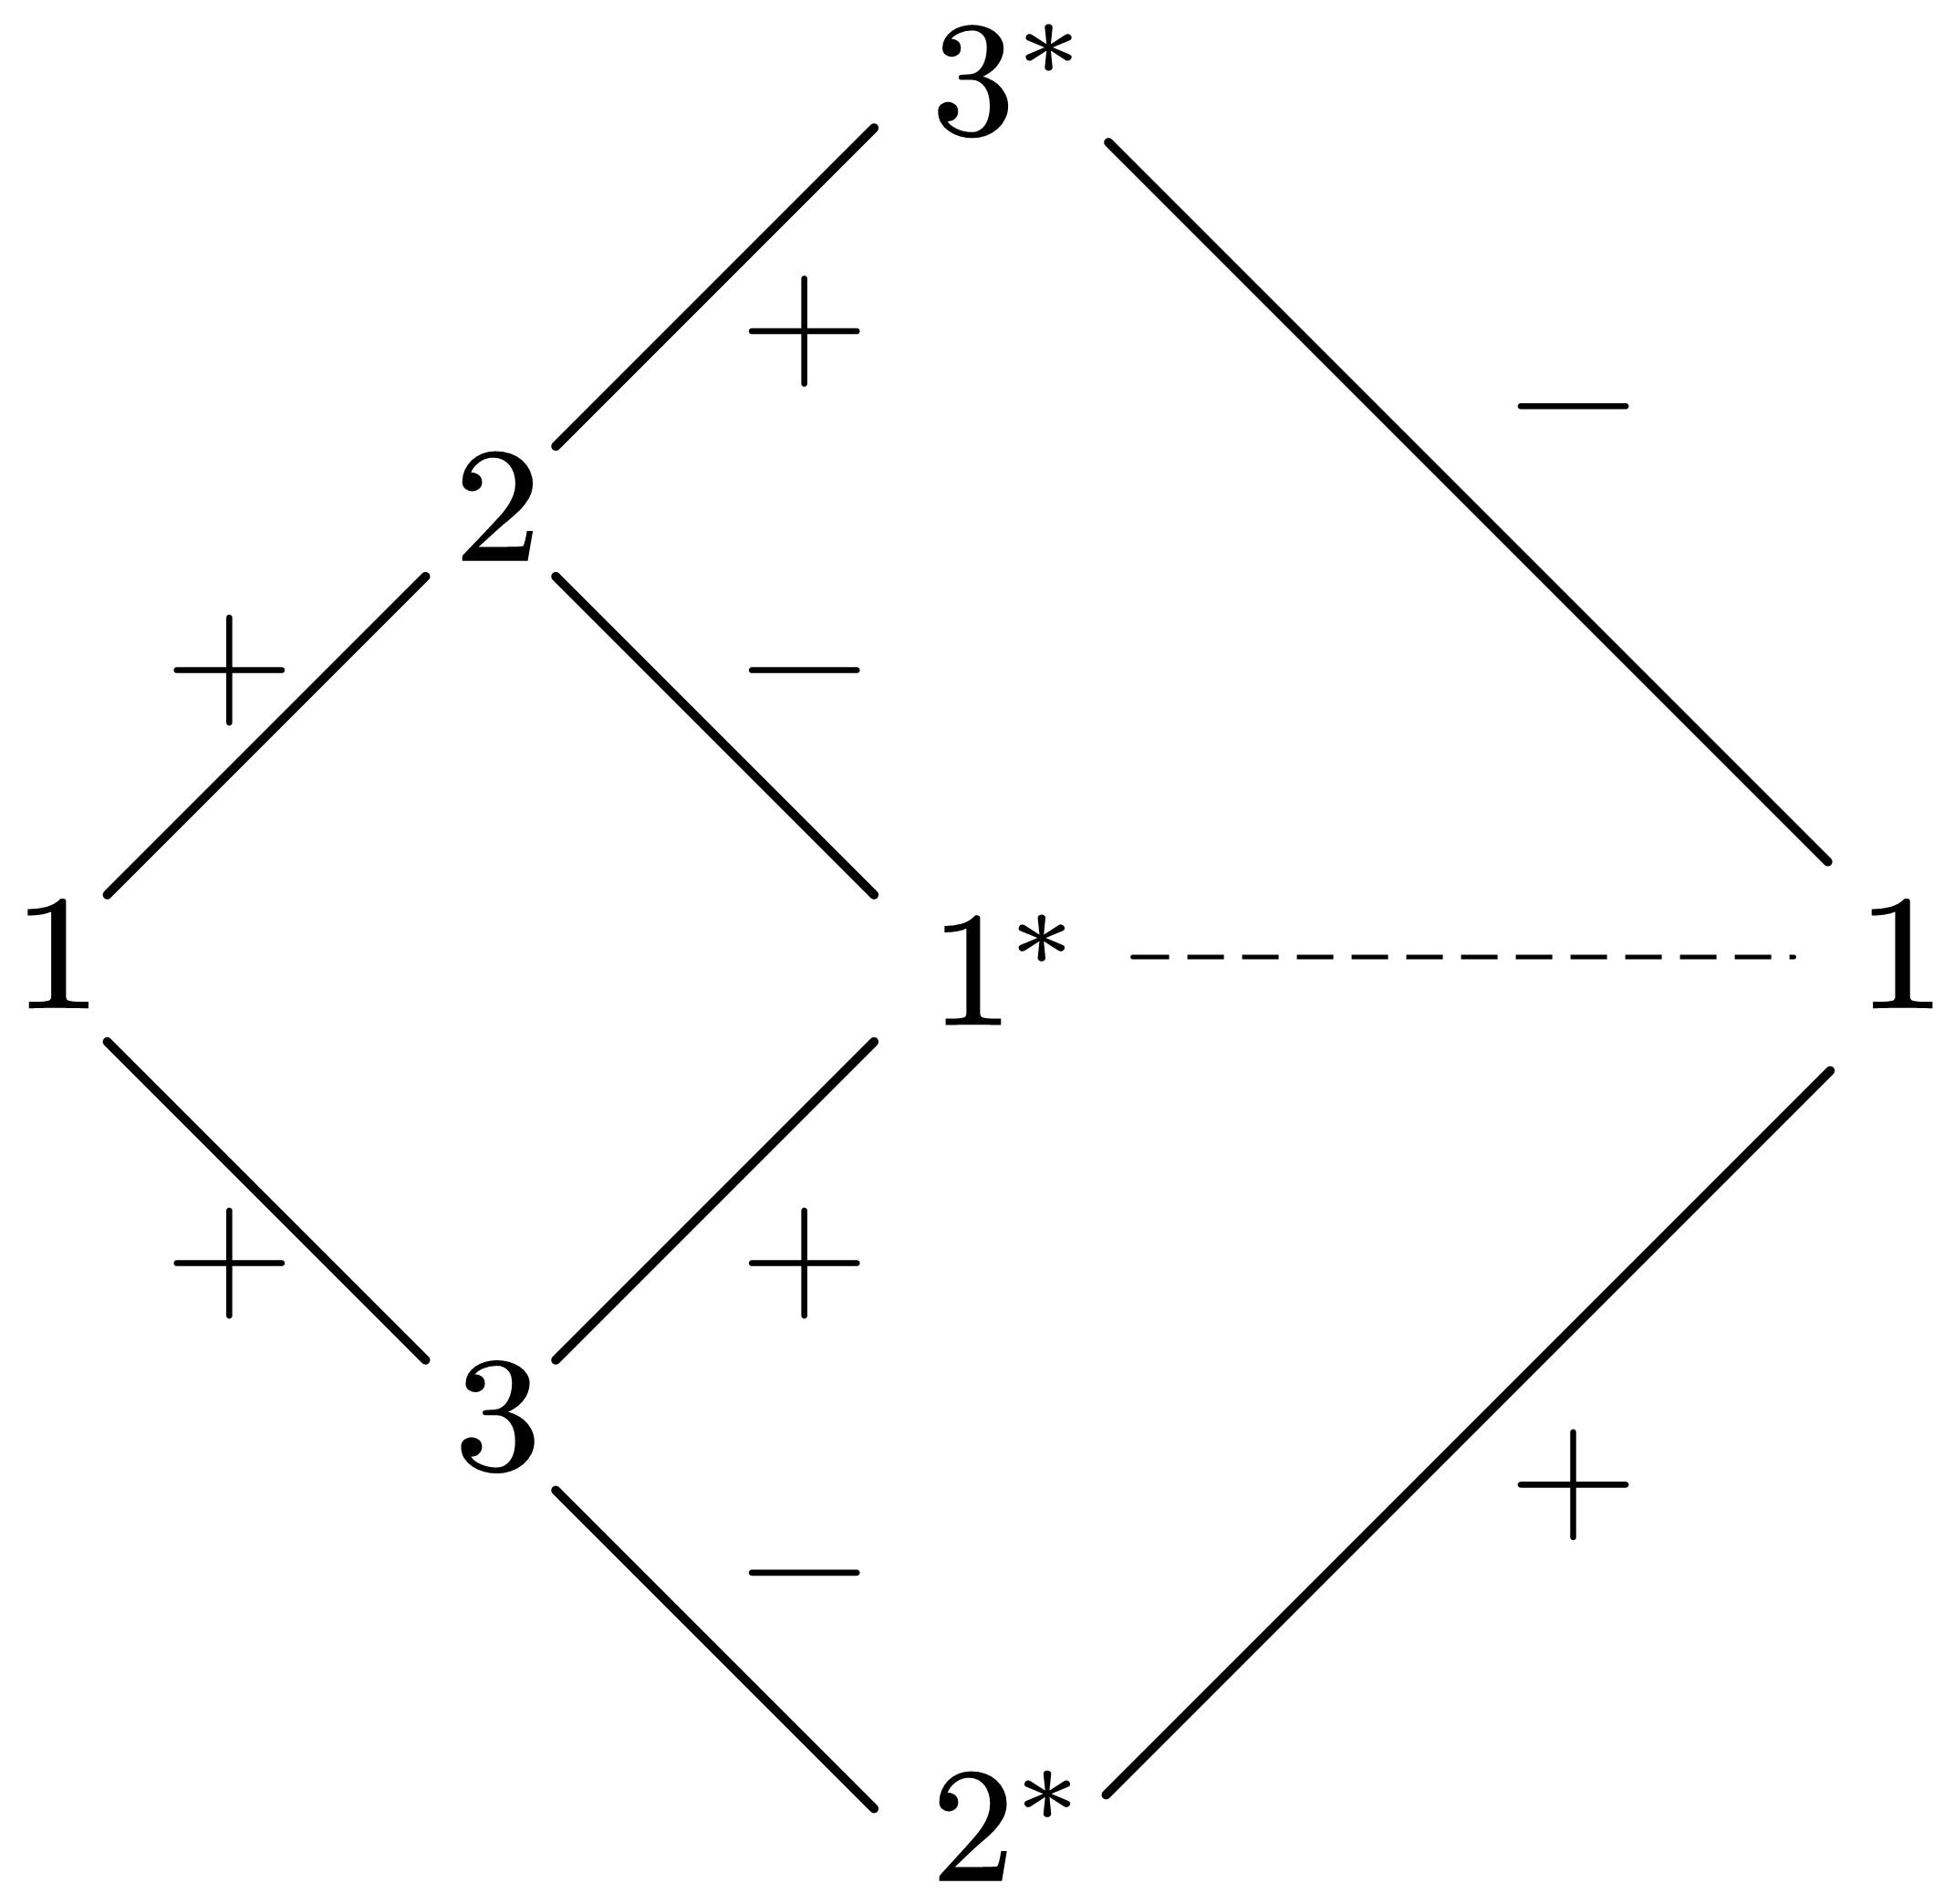
\includegraphics[scale=0.8]{./pictures/6.05/pictorial_representation_1.png}
		\captionof{figure}{Pictorial representation of the second term in $E^{(3)}_0$, where the order is $v_{ij}$, $v_{jk^*}$ and $v_{k^*i}$ from the left to the right. The plus and minus signs indicate whether the matrix elements between the two orbitals is $\pm \frac{\beta}{2}$.}\label{fig:exe5}
	\end{center}
	
	With the high symmetry, it is
	\begin{sequation}
		-2 \times \frac{1}{ (2\beta)^2 } \sum_{i=1}^3 \left[ v_{12} v_{23^*} v_{3^*1} + v_{13} v_{32^*} v_{2^*1} \right] = - \frac{3}{ 2\beta^2 } \left[ \frac{ \beta }{2} \times \frac{ \beta }{2} \times \left( - \frac{ \beta }{2} \right) + \frac{ \beta }{2} \times \left( - \frac{ \beta }{2} \right) \times \frac{ \beta }{2} \right] = \frac{3}{8\beta} .
	\end{sequation}	
	
	\end{solution}

	% 6.6
	\begin{exercise}
	Consider a cyclic polyene with $N = 4\nu+2$, $\nu=1$, $2$, ... carbons. Instead of assuming that all the bonds are identical, suppose they alternate in length. In the context of H{\"u}ckel theory this means that the resonance integrals between adjacent carbons are not all equal to $\beta$ but alternate between $\beta_1$ and $\beta_2$. For example, for benzene we have
	
	\begin{center}
	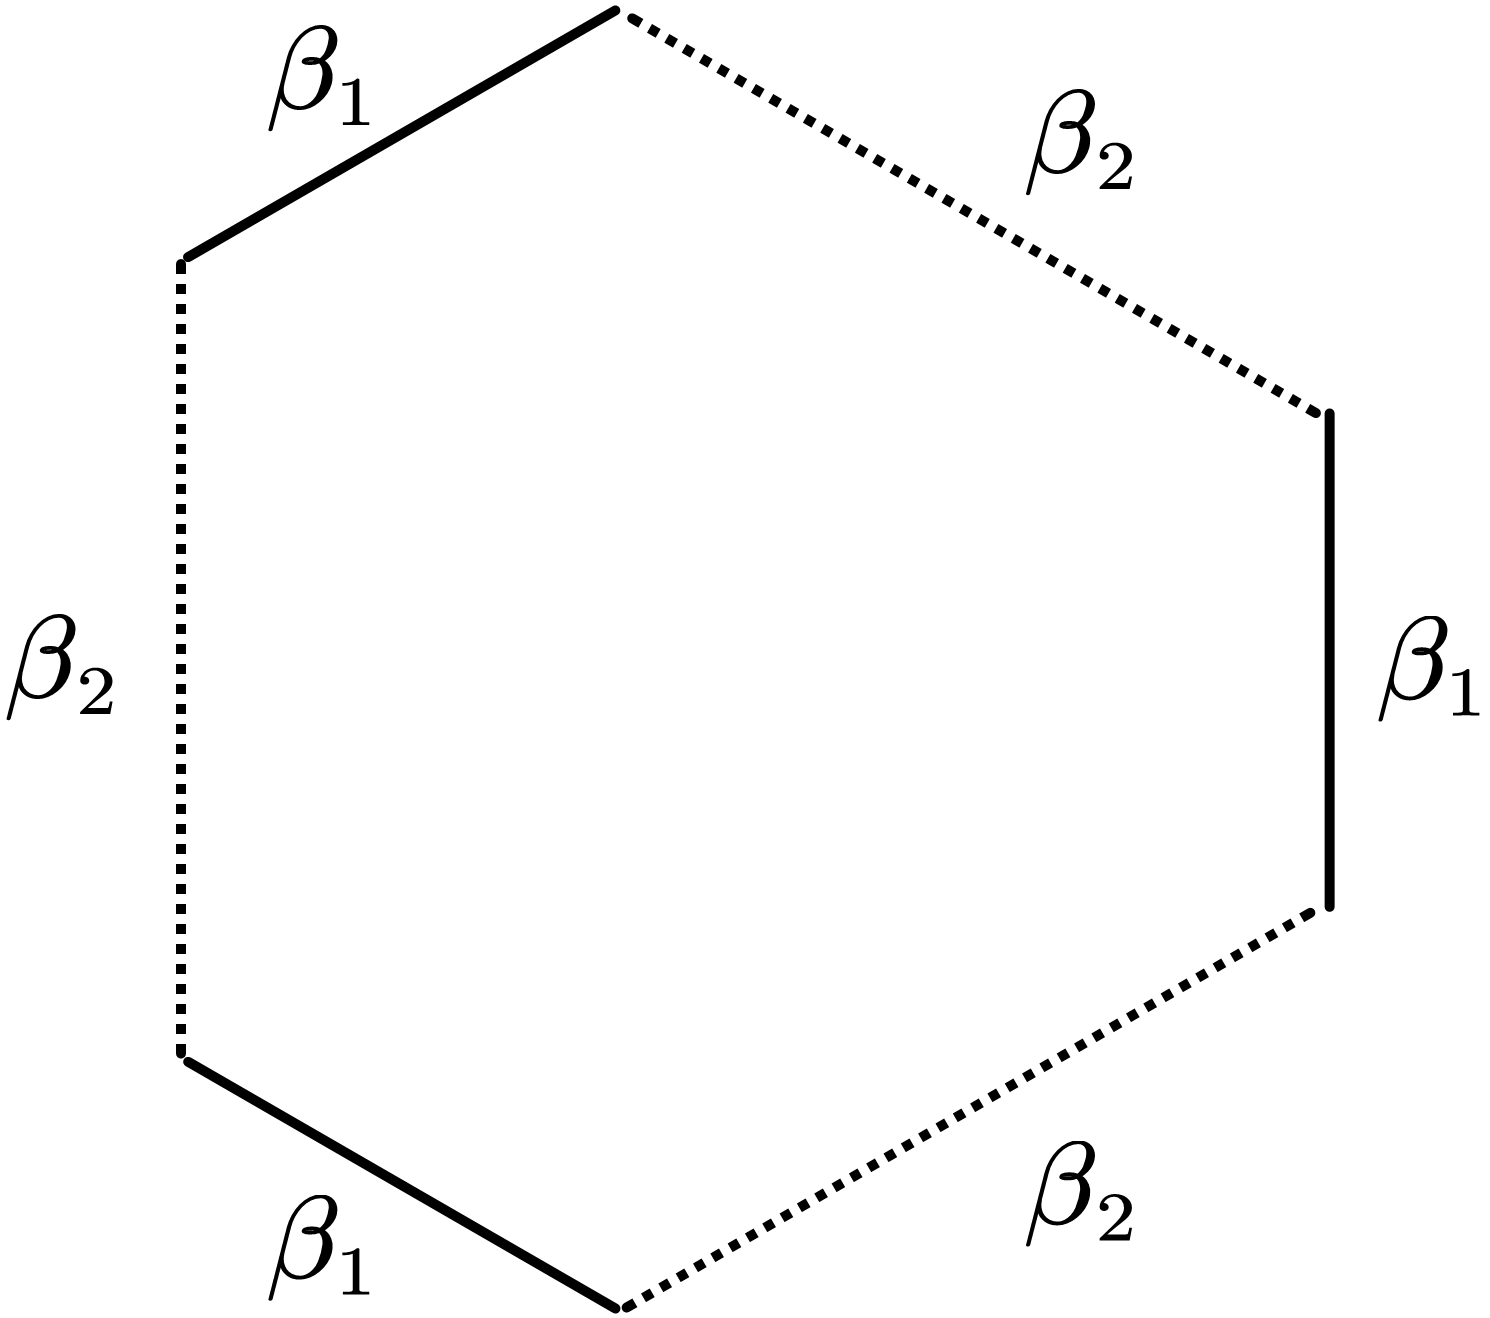
\includegraphics[scale=1.2]{./pictures/6.06/exercise_1.png}
	\end{center}
	
	Now it can be shown that the exact energy for a cyclic polyene of this type is
	\[
		\mathscr{E}_0 = N \alpha - 2 \sum_{j=-\nu}^\nu \left( \beta^2_1 + \beta^2_2 + 2 \beta_1 \beta_2 \cos{\frac{2j\pi}{2\nu+1}} \right)^{1/2}
	\]
	(see for example, L. Salem, {\it Molecular Orbital Theory of Conjugated Systems}, Benjamin, New York, 1966, pp.498-500). Note that when $\beta_1 = \beta_2 = \beta$, since $2\cos^2\theta=(1+\cos2\theta)$ and $\beta$ is negative, we recover
	\[
		\mathscr{E}_0 = N \alpha + 4 \beta \sum_{j=-\nu}^\nu \cos{\frac{j\pi}{2\nu+1}}
	\]
	which is the result quoted in Subsection 5.3.2. Also note that when $\beta_1=\beta$ but $\beta_2=0$, we have
	\[
		\mathscr{E}_0 = N \alpha + N \beta
	\]
	which is just the total energy of the polyene using the localized ethylenic description. The purpose of this exercise is to obtain the perturbation expansion for the resonance energy by expanding the exact energy in powers of $\beta_2/\beta_1$.
	\begin{enumerate}
	
	\item[a.] Show that for benzene ($\nu=1$) the exact ground state energy in the alternating short and long bond model is
	\[
		\mathscr{E}_0 = 6 \alpha + 2(\beta_1 + \beta_2) - 4 ( \beta^2_1 + \beta^2_2 - \beta_1 \beta_2 )^{1/2}
	\]
	Do this first by using the general expression and then by setting up the H{\"u}ckel matrix, diagonalizing it and adding up the occupied orbital energies. Note that when $\beta_1=\beta_2=\beta$ we recover our old result, $6\alpha+8\beta$.
	
	\item[b.] Setting $\beta_1 = \beta$ and $\beta_2/\beta_1=x$ show that the resonance energy of benzene can be written as
	\[
		E_R = 4 \beta ( \frac{1}{2}x - 1 + (1-x+x^2)^{1/2})
	\]
	Note that when $x=0$, $E_R=0$ and when $x=1$, $E_R=2\beta$ which is exact.
	
	\item[c.] Using the relation
	\[
		(1 + y)^{1/2} = 1 + \frac{1}{2} y - \frac{1}{8}y^2 + \frac{1}{16} y^3 - \frac{5}{128}y^4 + \cdots , \quad |y|<1
	\]	
	expand $E_R$ to fourth order in $x$ and thus show that
	\[
		E_R = \beta ( \frac{3}{2}x^2 + \frac{3}{4} x^3 + \frac{3}{32}x^4 + \cdots )
	\]
	Identifying the coefficient of $x^n$ with the $n$th-order perturbation result (i.e., $E^{(n)}_0$), we have
	\begin{align*}
		E^{(2)}_0 &= \frac{3}{2} \beta, \\
		E^{(3)}_0 &= \frac{3}{4} \beta, \\
		E^{(4)}_0 &= \frac{3}{32} \beta.
	\end{align*}
	Note that $E^{(2)}_0$ and $E^{(3)}_0$ agree with our previously calculated values. This derivation provides some insight into the poor convergence of the perturbation expansion of the resonance energy of benzene. Basically, the perturbation expansion converges rapidly when $x$ is small. However, for our problem $x$ is equal to unity.
	
	The resonance energy calculated up to $M$th-order as a function of $M$ is shown below. Note the oscillatory convergence towards the exact value of $2\beta$. The method used above to obtain $E^{(n)}_0$ for $n=2,3,4$ becomes extremely laborious for larger $n$. The results below were calculated by first showing that $E^{(n)}_0 = 4\beta C^{-1/2}_n(1/2)$, where $C^{-1/2}_n(x)$ is a Gegenbauer polynomial of degree $n$ and order $-\frac{1}{2}$, and then using the recursive properties of these polynomials, to show that
	\[
		(n+1)E^{(n+1)}_0 = (n-1) E^{(n)}_0 - (n-2) E^{(n-1)}_0.
	\]
	
	\begin{center}
	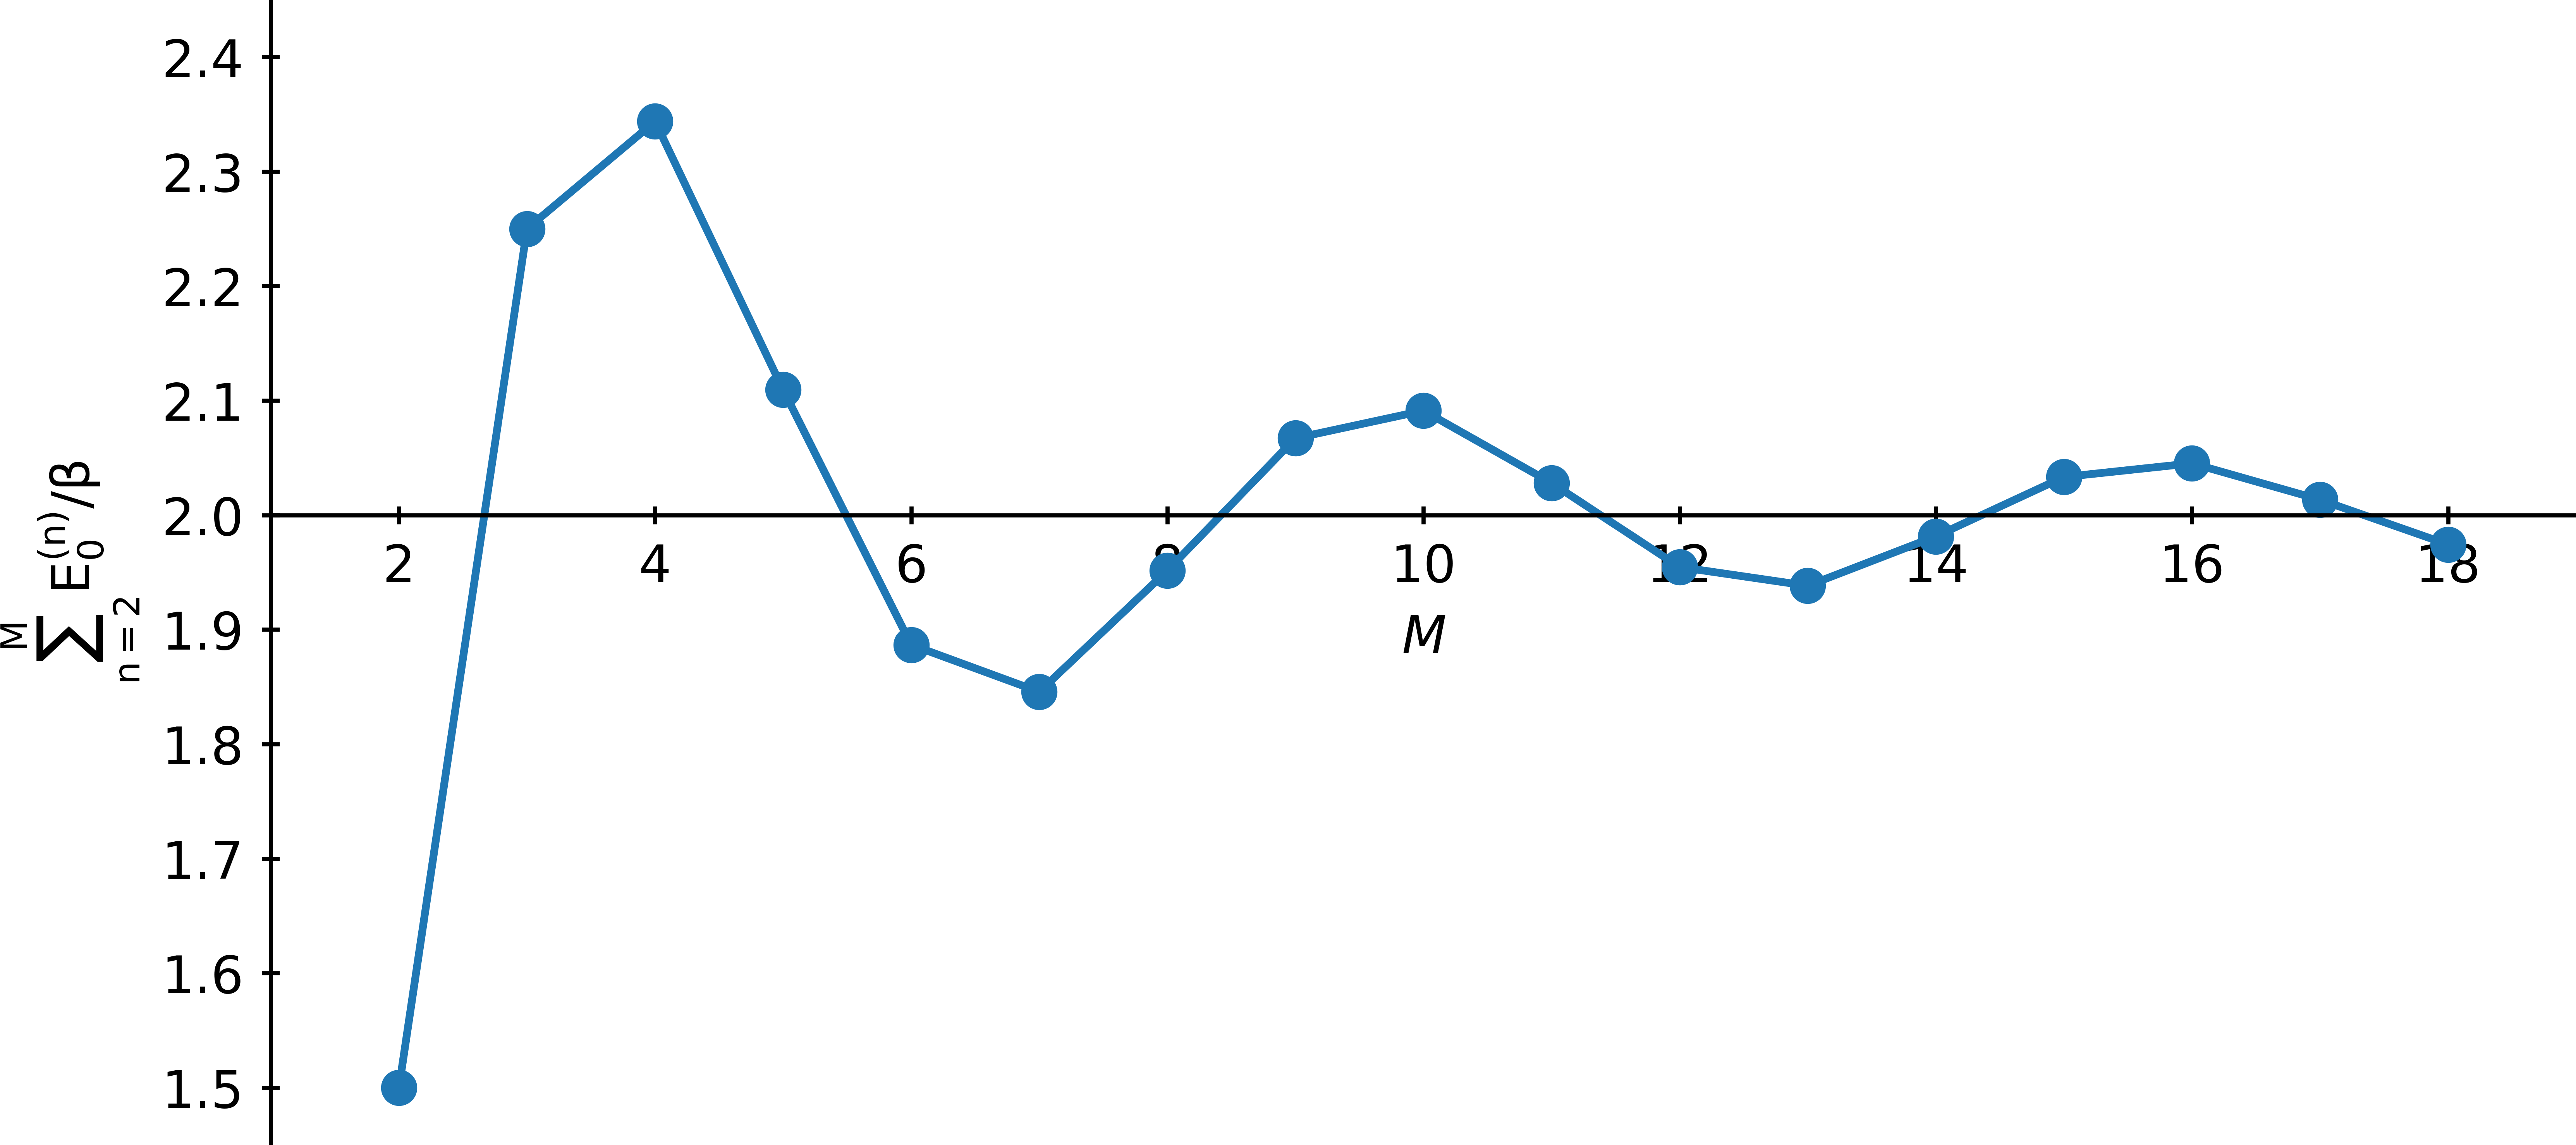
\includegraphics[scale=0.84]{./pictures/6.06/gegenbauer.png}
	\end{center}
	
	\end{enumerate}
	
	\end{exercise}
	
	\begin{solution}

	\begin{itemize}
	
	\item[a.] Using the general expression and note that $\beta_1 \le 0$ and $\beta_2 \le 0$, we get that
	\begin{align*}
		\mathscr{E}_0({\rm benzene}) &= 6 \times \alpha - 2 \sum_{ j=-1 }^1 \left( \beta^2_1 + \beta^2_2 + 2 \beta_1 \beta_2 \cos{\frac{2j\pi}{ 2 \times 1 + 1 }} \right)^{1/2} \\
		&= 6\alpha - 2 \left( \beta^2_1 + \beta^2_2 + 2 \beta_1 \beta_2 \cos{\frac{-2\pi}{ 3 }} \right)^{1/2} \\
		&\hspace{2em} - 2 \left( \beta^2_1 + \beta^2_2 + 2 \beta_1 \beta_2 \cos{\frac{0\pi}{ 3 }} \right)^{1/2} - 2 \left( \beta^2_1 + \beta^2_2 + 2 \beta_1 \beta_2 \cos{\frac{2\pi}{ 3 }} \right)^{1/2} \\
		&= 6\alpha - 2\left( \beta^2_1 + \beta^2_2 - \beta_1 \beta_2 \right)^{1/2} + 2\left( \beta_1 + \beta_2 \right) - 2\left( \beta^2_1 + \beta^2_2 - \beta_1 \beta_2 \right)^{1/2}.
	\end{align*}
	In a nut shell,
	\begin{sequation}
		\mathscr{E}_0({\rm benzene}) = 6\alpha + 2\left( \beta_1 + \beta_2 \right) - 4\left( \beta^2_1 + \beta^2_2 - \beta_1 \beta_2 \right)^{1/2} .
	\end{sequation}
	
	At this time, we should remember that the H{\"u}ckel matrix is 
	\[
		\HH = \begin{pmatrix}
			\alpha & \beta_2 & 0 & 0 & 0 & \beta_1 \\
			\beta_2& \alpha  & \beta_1 & 0 & 0 & 0 \\
			0 & \beta_1& \alpha  & \beta_2 & 0 & 0 \\
			0 & 0 & \beta_2& \alpha  & \beta_1 & 0 \\
			0 & 0 & 0 & \beta_1& \alpha  & \beta_2 \\
			\beta_1 & 0 & 0 & 0 & \beta_2 & \alpha
		\end{pmatrix}.
	\]
	Its eigen function is
	\[
		\det{\HH-\varepsilon\I} = (\beta^2_1 - \beta_1 \beta_2 + \beta^2_2 - (\alpha - \varepsilon)^2)^2 (\alpha - \beta_1 - \beta_2 - \varepsilon) (\alpha + \beta_1 + \beta_2 - \varepsilon) = 0,
	\]
	and there are six roots:
	\begin{align*}
		\varepsilon_1 &= \alpha + \beta_1 + \beta_2 , \\
		\varepsilon_2 = \varepsilon_3 &= \alpha - \sqrt{ \beta^2_1 - \beta_1 \beta_2 + \beta^2_2 }, \\
		\varepsilon_4 = \varepsilon_5 &= \alpha + \sqrt{ \beta^2_1 - \beta_1 \beta_2 + \beta^2_2 }, \\
		\varepsilon_6 &= \alpha - \beta_1 - \beta_2 .
	\end{align*}
	Thus,
	\begin{sequation}
		\mathscr{E}^\prime_0({\rm benzene}) = 2\varepsilon_1 + 2\varepsilon_2 + 2\varepsilon_3 = 6\alpha + 2\left( \beta_1 + \beta_2 \right) - 4\left( \beta^2_1 + \beta^2_2 - \beta_1 \beta_2 \right)^{1/2} .
	\end{sequation}
	It equals the results obtained by using the general expression.
	
	\item[b.] The verification is direct. With $\beta_1 = \beta$, $\beta_2 = x\beta_1 = x\beta$, we get that
	\begin{align*}
		E_R &= \mathscr{E}_0({\rm benzene}) - E_0 = 6\alpha + 2\left( \beta + x \beta \right) - 4\left( \beta^2 + ( x \beta )^2 - x \beta^2 \right)^{1/2} - ( 6\alpha + 6\beta ) \\
		&= -4\beta + 2x \beta + 4\beta \left( 1 + x^2 - x \right)^{1/2} = 4\beta \left( \frac{x}{2} - 1 + \left( 1 + x^2 - x \right)^{1/2} \right)
	\end{align*}
	
	\item[c.] When $0 \le x \le 1$, $-\frac{1}{4} \le x^2-x \le 0$, thus we obtain that
	\begin{align*}
		E_R &= 4\beta \left( \frac{x}{2} - 1 + \left( 1 + x^2 - x \right)^{1/2} \right) = 4\beta \left[ \frac{x}{2} - 1 + \left( 1 + \left( x^2 - x \right) \right)^{1/2} \right] \\
		&= 4\beta \left[ \frac{x}{2} - 1 + 1 + \frac{1}{2} \left( x^2 - x \right) - \frac{1}{8} \left( x^2 - x \right)^2 + \frac{1}{16} \left( x^2 - x \right)^3 - \frac{5}{128} \left( x^2 - x \right)^4 + \cdots \right] \\
		&= 4\beta \left[ \frac{x}{2} + \frac{1}{2} \left( - x + x^2 \right) - \frac{1}{8} \left( x^2 - 2 x^3 + x^4 \right)  \right. \\
		&\hspace{4em} \left. + \frac{1}{16} \left( - x^3 + 3 x^4 - 3 x^5 + x^6 \right) - \frac{5}{128} \left( x^4 - 4x^5 + 6x^6 - 4x^7 + x^8 \right) + \cdots \right] \\
		&= 4\beta \left[ \left( \frac{1}{2} - \frac{1}{2} \right) x + \left( \frac{1}{2} - \frac{1}{8} \right) x^2 + \left( \frac{1}{4} - \frac{1}{16} \right) x^3 + \left( - \frac{1}{8} + \frac{3}{16} - \frac{5}{128} \right) x^4 + \cdots \right] \\
		&= \beta \left( \frac{3}{2} x^2 + \frac{3}{4} x^3 + \frac{3}{32} x^4 + \cdots \right) .
	\end{align*}
	
	In fact, the Gegenbauer polynomials $C^\lambda_n(x)$ can be generated by $(1-2xt+t^2)^{-\lambda}$, viz.,
	\[
		(1-2xt+t^2)^{-\lambda} = \sum_{ n=0 }^\infty C^\lambda_n (x) t^n, \, \forall t \in (-1,1), x \in (-1,1).
	\]
	Let $\lambda=-\frac{1}{2}$ and $x=\frac{1}{2}$, we obtain that
	\[
		( 1 - t + t^2 )^{\frac{1}{2}} = \sum_{ n=0 }^\infty C^{-\frac{1}{2}}_n \left( \frac{1}{2} \right) t^n.
	\]
	Thus, with 
	\[
		C^\lambda_0(x) = 1 , \quad C^\lambda_1(x) = 2 \lambda x ,
	\]	
	we find that	
	\[
		\sum_{ n=0 }^\infty C^{-\frac{1}{2}}_n \left( \frac{1}{2} \right) t^n = C^{-\frac{1}{2}}_0 \left( \frac{1}{2} \right) + C^{-\frac{1}{2}}_0 \left( \frac{1}{2} \right) t + \sum_{ n=2 }^\infty C^{-\frac{1}{2}}_n \left( \frac{1}{2} \right) t^n = 1 - \frac{t}{2} + \sum_{ n=2 }^\infty C^{-\frac{1}{2}}_n \left( \frac{1}{2} \right) t^n.
	\]
	
	Hence, we get
	\begin{sequation}
		E_R = 4\beta \left( \frac{x}{2} - 1 + \left( 1 - x + x^2 \right)^{1/2} \right) = 4\beta \sum_{ n=2 }^\infty C^{-\frac{1}{2}}_n \left( \frac{1}{2} \right) x^n.
	\end{sequation}
	It equals
	\begin{sequation}
		E^{(n)}_0 = 4\beta C^{-\frac{1}{2}}_n \left( \frac{1}{2} \right), \, n = 2, 3, 4, \cdots.
	\end{sequation}
	
	Due to the recurrence relation of Gegenbauer polynomials,
	\[
		(n+1)C^\lambda_{n+1}(x) = 2(n+\lambda) x C^\lambda_n(x) - ( n + 2\lambda - 1 ) C^\lambda_{n-1}(x), \, \forall n \ge 1, 
	\]
	we know that for $n=2,3,\cdots$,
	\begin{align*}
		(n+1)E^{(n+1)}_0 &= (n+1) \times 4\beta C^{-\frac{1}{2}}_{n+1} \left( \frac{1}{2} \right) = 4\beta (n+1) C^{-\frac{1}{2}}_{n+1} \left( \frac{1}{2} \right) \\
		&= 4\beta \left[ 2\left( n - \frac{1}{2} \right) \frac{1}{2} C^{ -\frac{1}{2} }_n \left( \frac{1}{2} \right) - \left( n + 2 \times \left( -\frac{1}{2} \right) - 1 \right) C^{ -\frac{1}{2} }_{n-1}\left( \frac{1}{2} \right) \right] \\
		&= 4\beta \left[ \left( n - \frac{1}{2} \right) C^{ - \frac{1}{2} }_n\left( \frac{1}{2} \right) - ( n - 2 ) C^{ - \frac{1}{2}}_{n-1}\left( \frac{1}{2} \right) \right] \\
		&= \left( n - \frac{1}{2} \right) 4\beta C^{ -\frac{1}{2} }_n\left( \frac{1}{2} \right) - ( n - 2 ) 4\beta C^{ -\frac{1}{2} }_{n-1}\left( \frac{1}{2} \right) \\
		&= \left( n - \frac{1}{2} \right) E^{(n)}_0 - ( n - 2 ) E^{(n-1)}_0.
	\end{align*}
	
	\end{itemize}
	
	Remark: You can read some introduction about Gegenbauer polynomials from WIKIPEDIA, whose url is \url{https://en.wikipedia.org/wiki/Gegenbauer_polynomials}.	
		
	\end{solution}
	
	\sectionstar{Diagrammatic Representation of Orbital Perturbation Theory}
	
	% 6.7
	\begin{exercise}
	Find the fourth-order energy for a closed-shell cyclic polyene.
	\begin{enumerate}
	
	\item[a.] Show that
	
	\begin{center}
	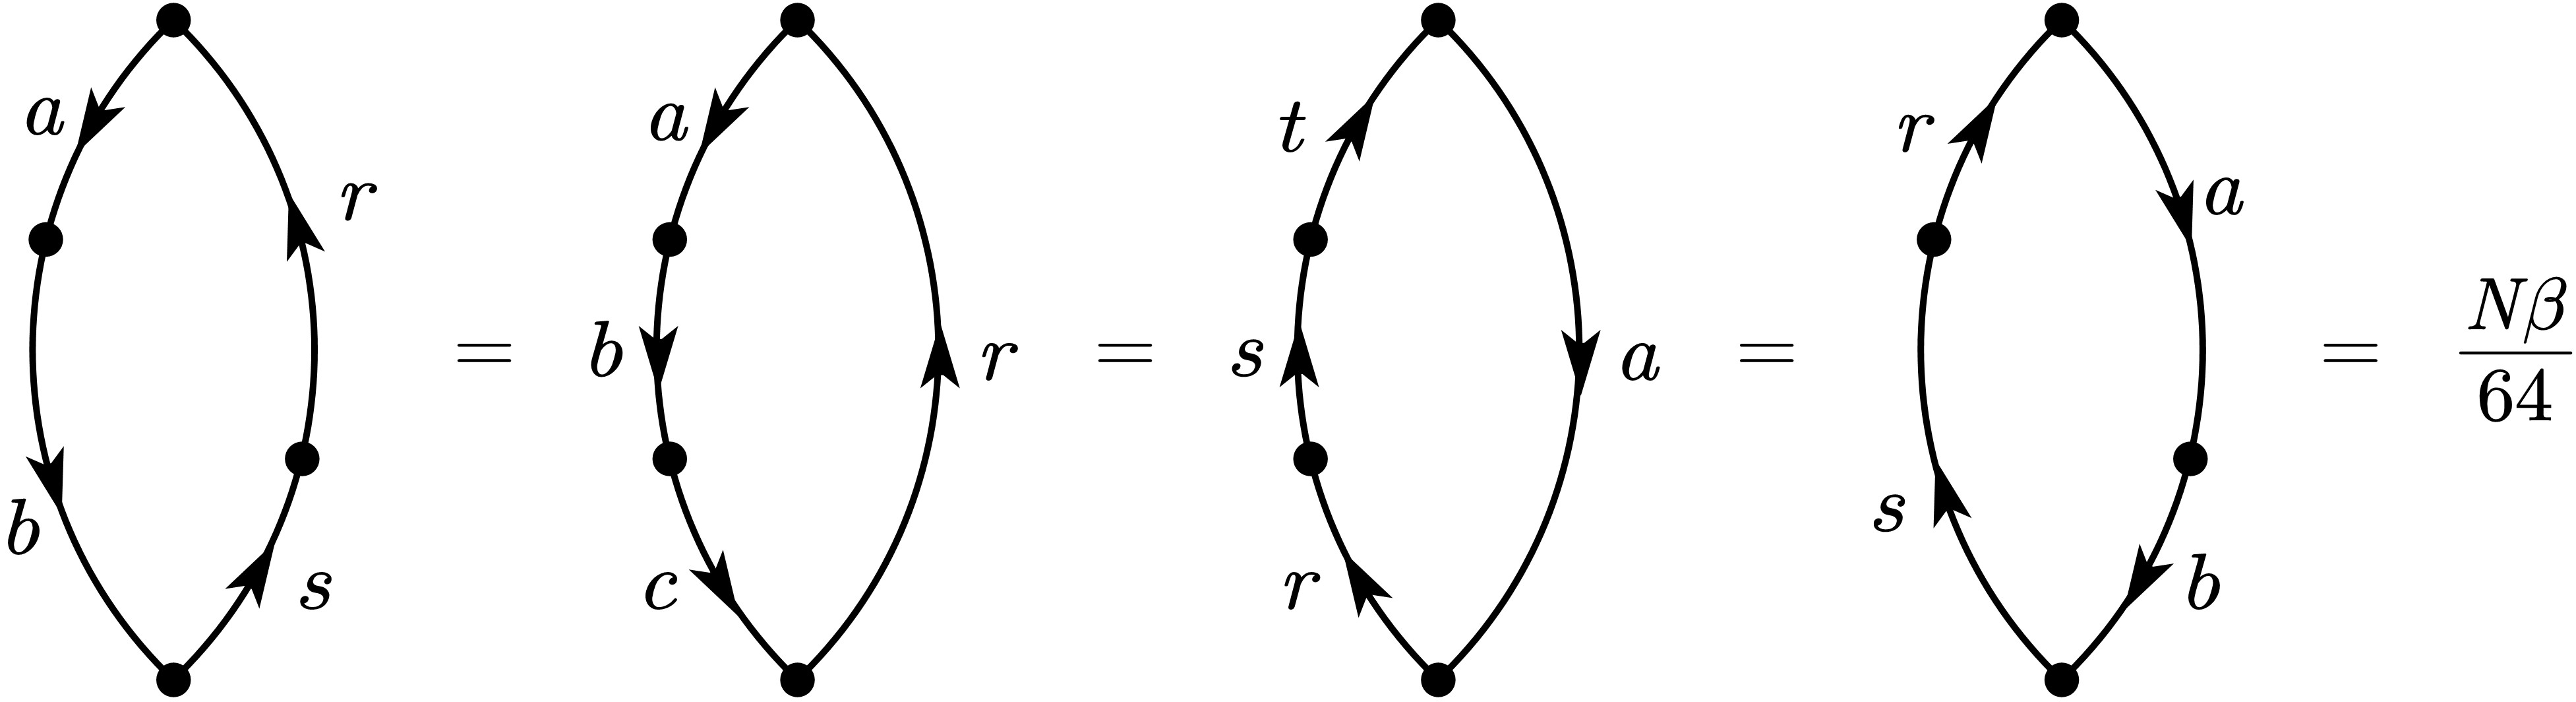
\includegraphics[scale=0.84]{./pictures/6.07/exercise_1.png}
	\end{center}
	
	and
	
	\begin{center}
	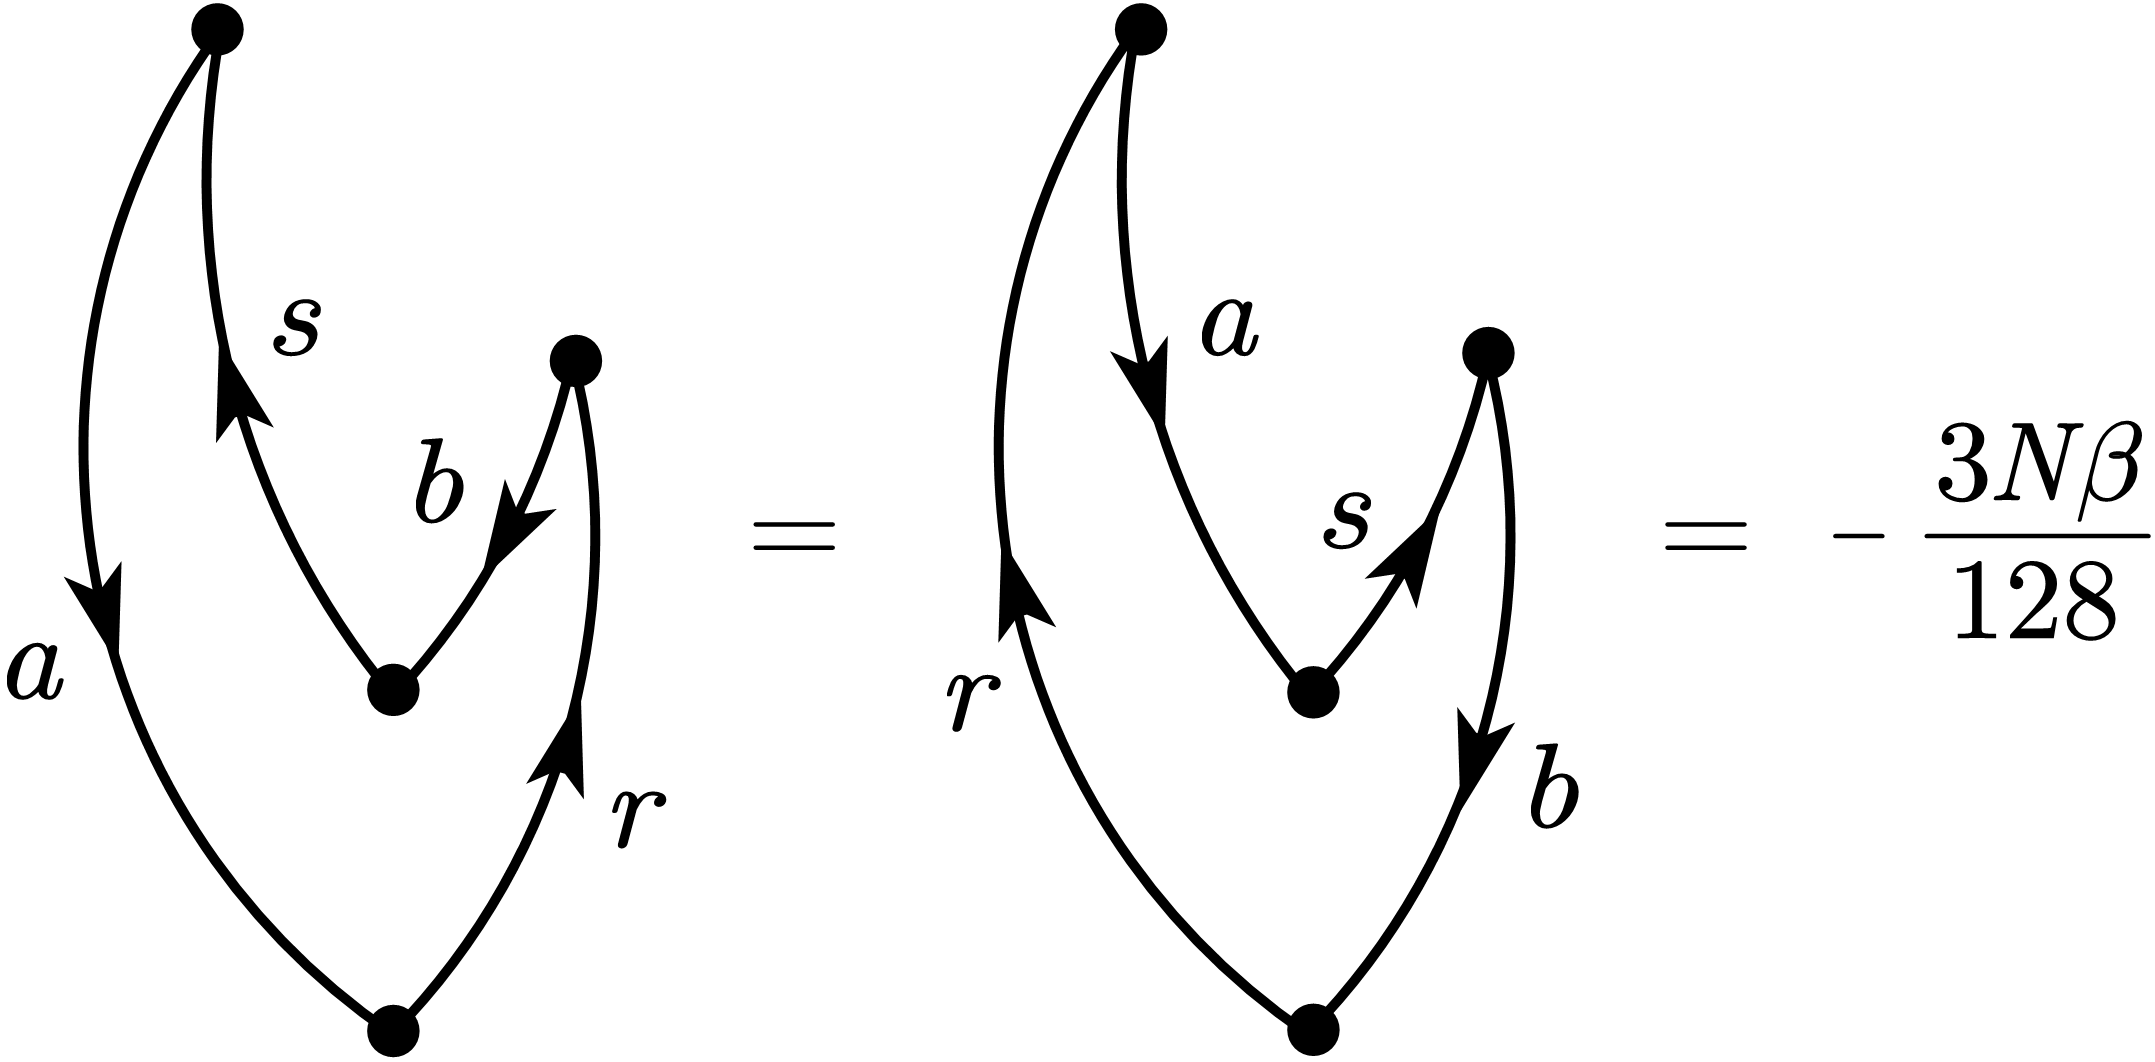
\includegraphics[scale=0.84]{./pictures/6.07/exercise_2.png}
	\end{center}
	
	so that
	\[
		E^{(4)}_0 = \frac{N\beta}{64}
	\]
	Thus the resonance energy calculated for a cyclic polyene with $N>6$ up to fourth order is (1/4 + 1/64)$N\beta = 0.2656N\beta$, which compares very favorably with the asymptotically exact value of 0.2732$\beta$ (i.e., 97\%).
	
	\item[b.] For benzene, show that the diagrammatic result for the fourth-order energy agrees with the independently calculated result found in Exercise 6.6.
	
	\end{enumerate}		
	
	\end{exercise}
	
	\begin{solution}
	
	\begin{itemize}	
	
	\item[a.] Firstly, we list all diagrams of the fourth-order energy. 	
	\begin{center}
	\begin{tabular}{ccc}
	
		\begin{minipage}{0.22\linewidth}
		\centering
		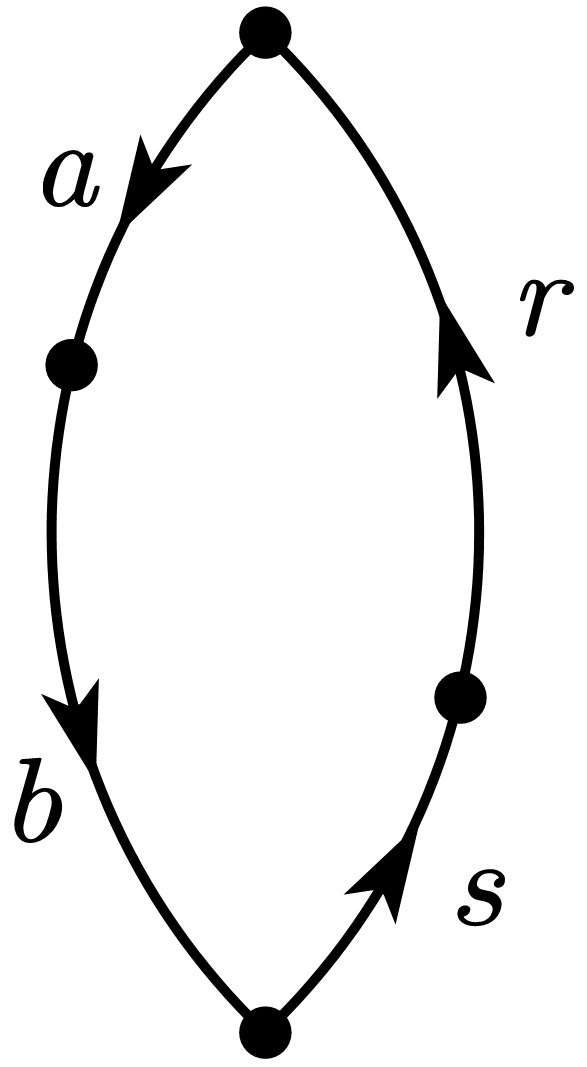
\includegraphics[scale=1.0,trim=0 -4 0 -4]{./pictures/6.07/diagram_1.png}
		\end{minipage} &
		
		\begin{minipage}{0.22\linewidth}
		\centering
		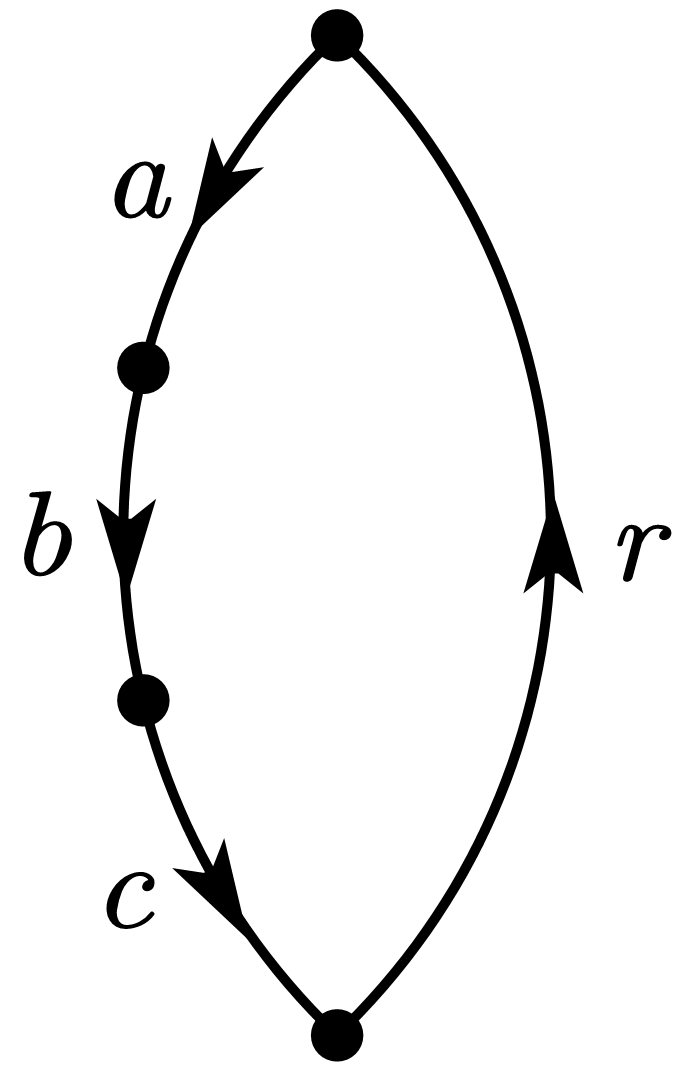
\includegraphics[scale=1.0,trim=0 -4 0 -4]{./pictures/6.07/diagram_2.png}
		\end{minipage} &
		
		\begin{minipage}{0.22\linewidth}
		\centering
		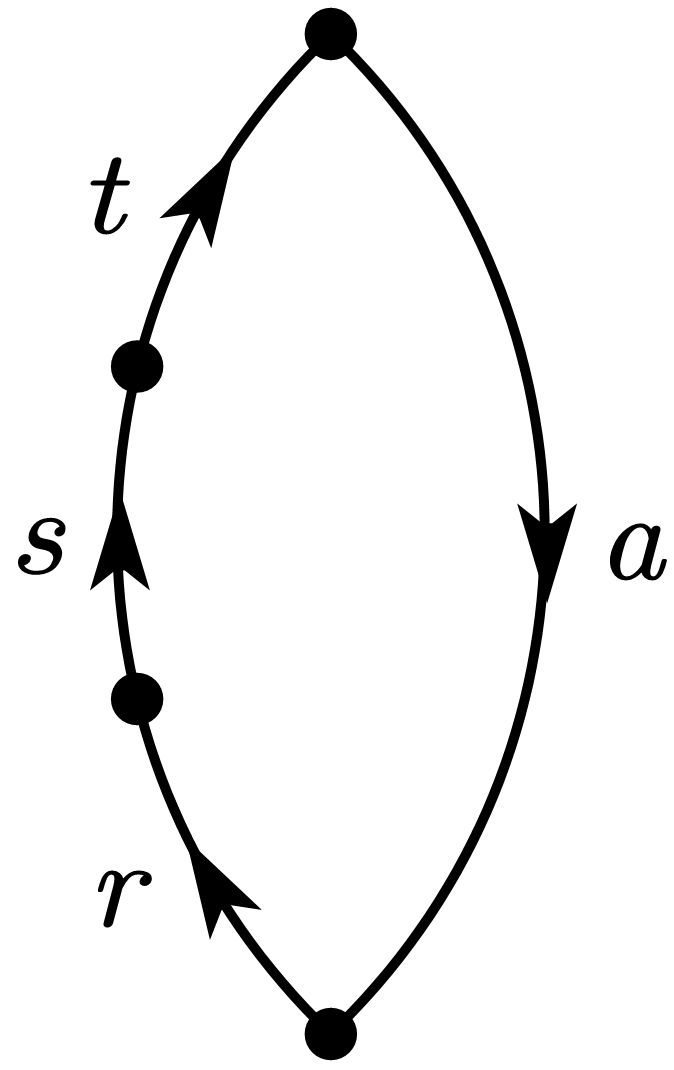
\includegraphics[scale=1.0,trim=0 -4 0 -4]{./pictures/6.07/diagram_3.png}
		\end{minipage} \\
		
		\begin{minipage}{0.22\linewidth}
		\centering
		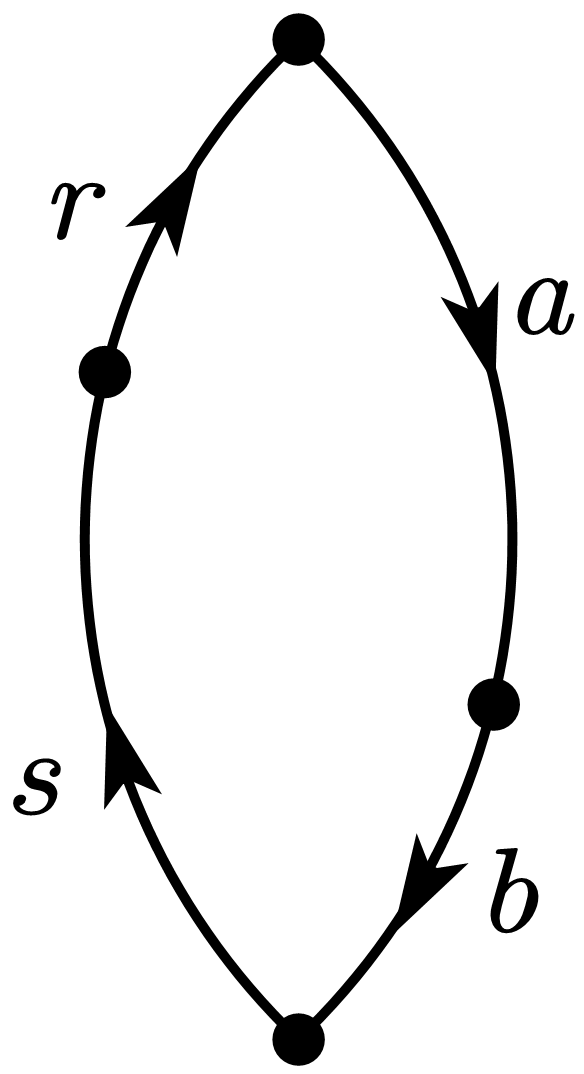
\includegraphics[scale=1.0,trim=0 -4 0 -4]{./pictures/6.07/diagram_4.png}
		\end{minipage} &
			
		\begin{minipage}{0.22\linewidth}
		\centering
		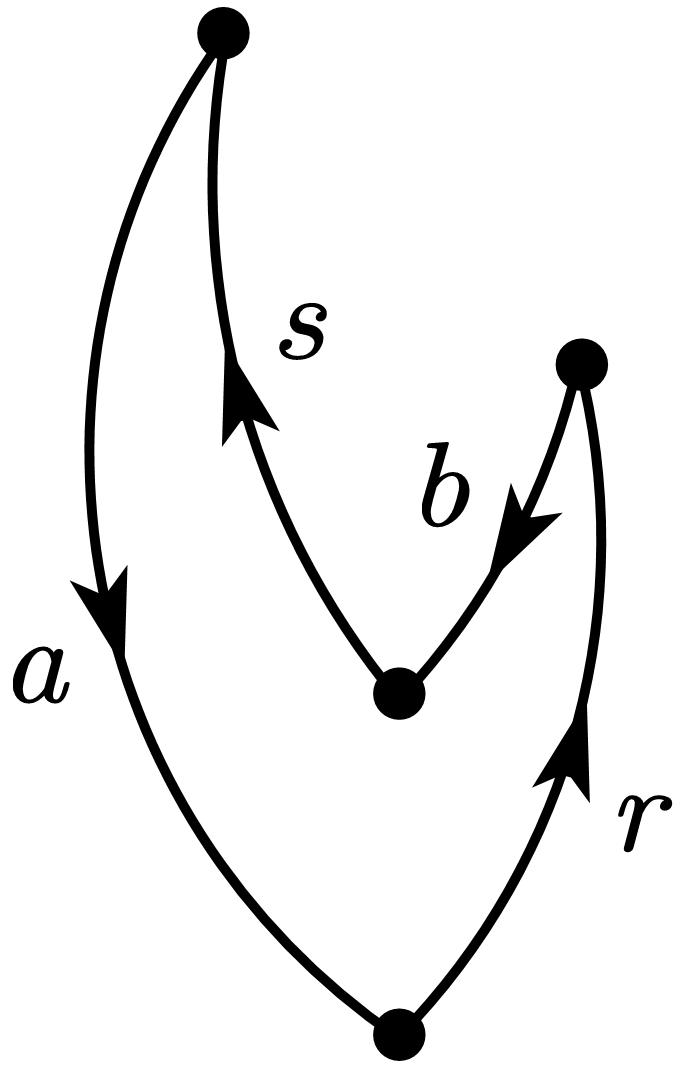
\includegraphics[scale=1.0,trim=0 -4 0 -4]{./pictures/6.07/diagram_5.png}
		\end{minipage} &
		
		\begin{minipage}{0.22\linewidth}
		\centering
		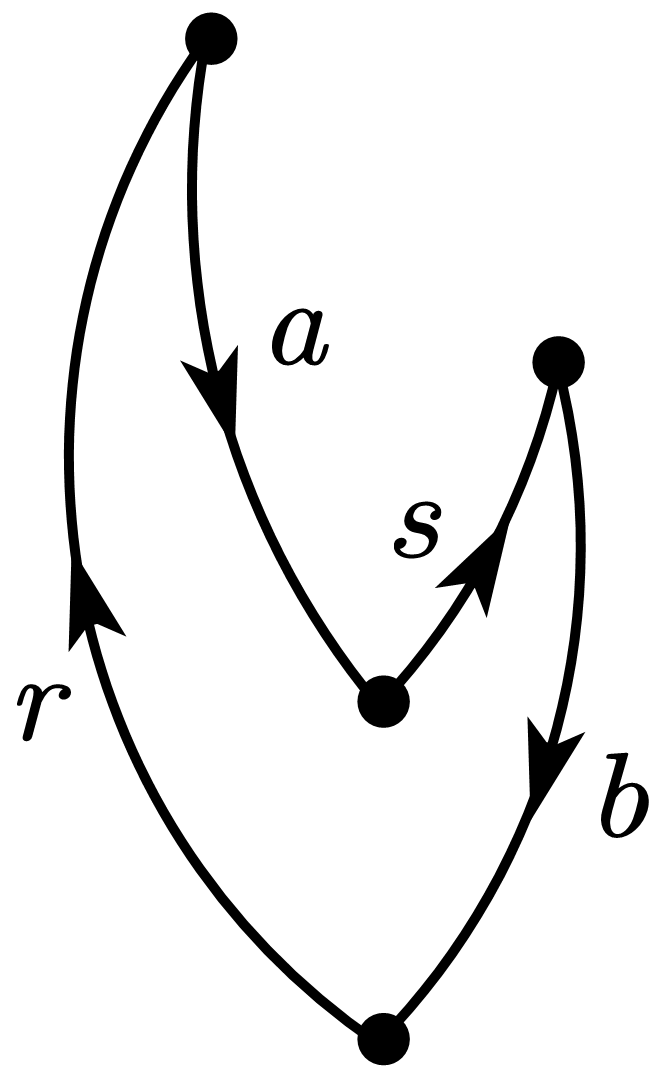
\includegraphics[scale=1.0,trim=0 -4 0 -4]{./pictures/6.07/diagram_6.png}
		\end{minipage}
		
	\end{tabular}
	\captionof{figure}{All fourth-order diagrams.}\label{fig:exe7_1}
	\end{center}
	
	Note that when $N>6$, $(i+3)^*$ cannot interact with $i$, and when $N=6$, $1^*$ cannot interact with $1$, either. Thus, there is no essential difference in the shape and properties between the case of $N > 6$ and $N=6$. It is enough to draw the pictorial representation of benzene ($N=6$) in order to get the same result of $N>6$. The pictorial representation of benzene can be seen in \Figref{fig:exe7_2}.
	
	\begin{center}
	\begin{tabular}{ccc}
	
		\begin{minipage}{0.3\linewidth}
		\centering
		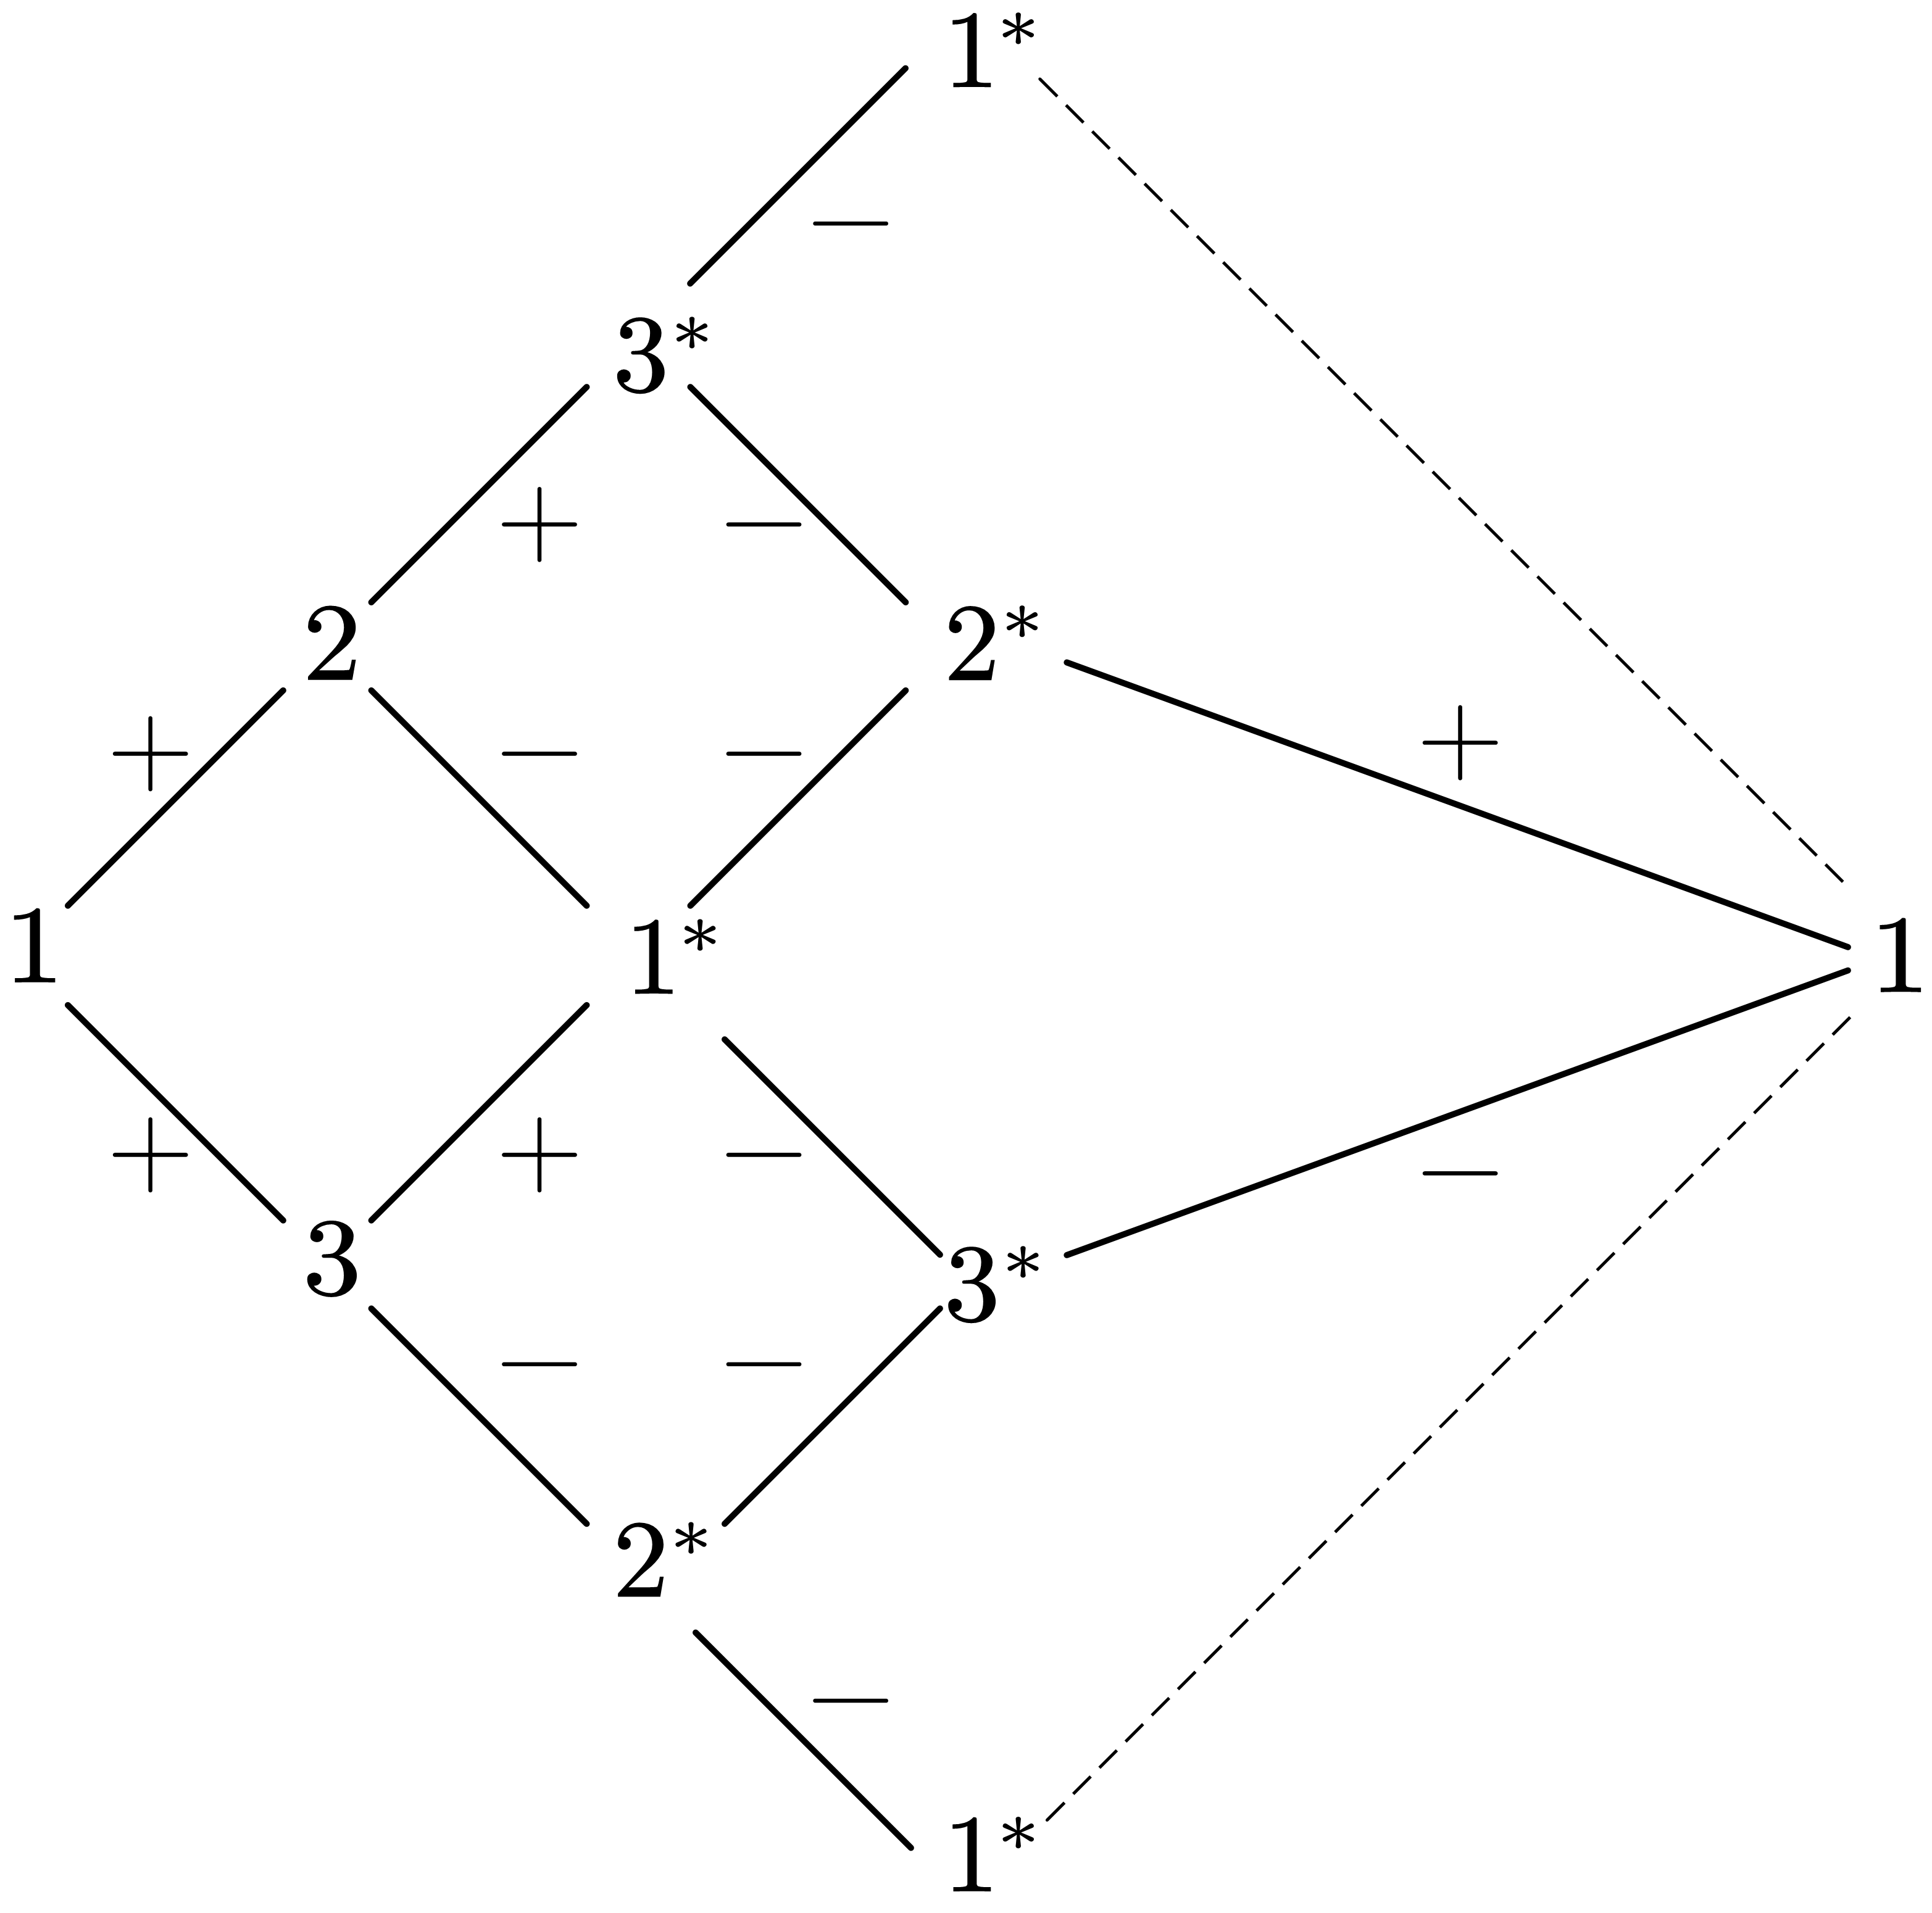
\includegraphics[scale=0.5,trim=0 -8 0 -8]{./pictures/6.07/pictorial_representation_1.png}
		\end{minipage} &
		
		\begin{minipage}{0.3\linewidth}
		\centering
		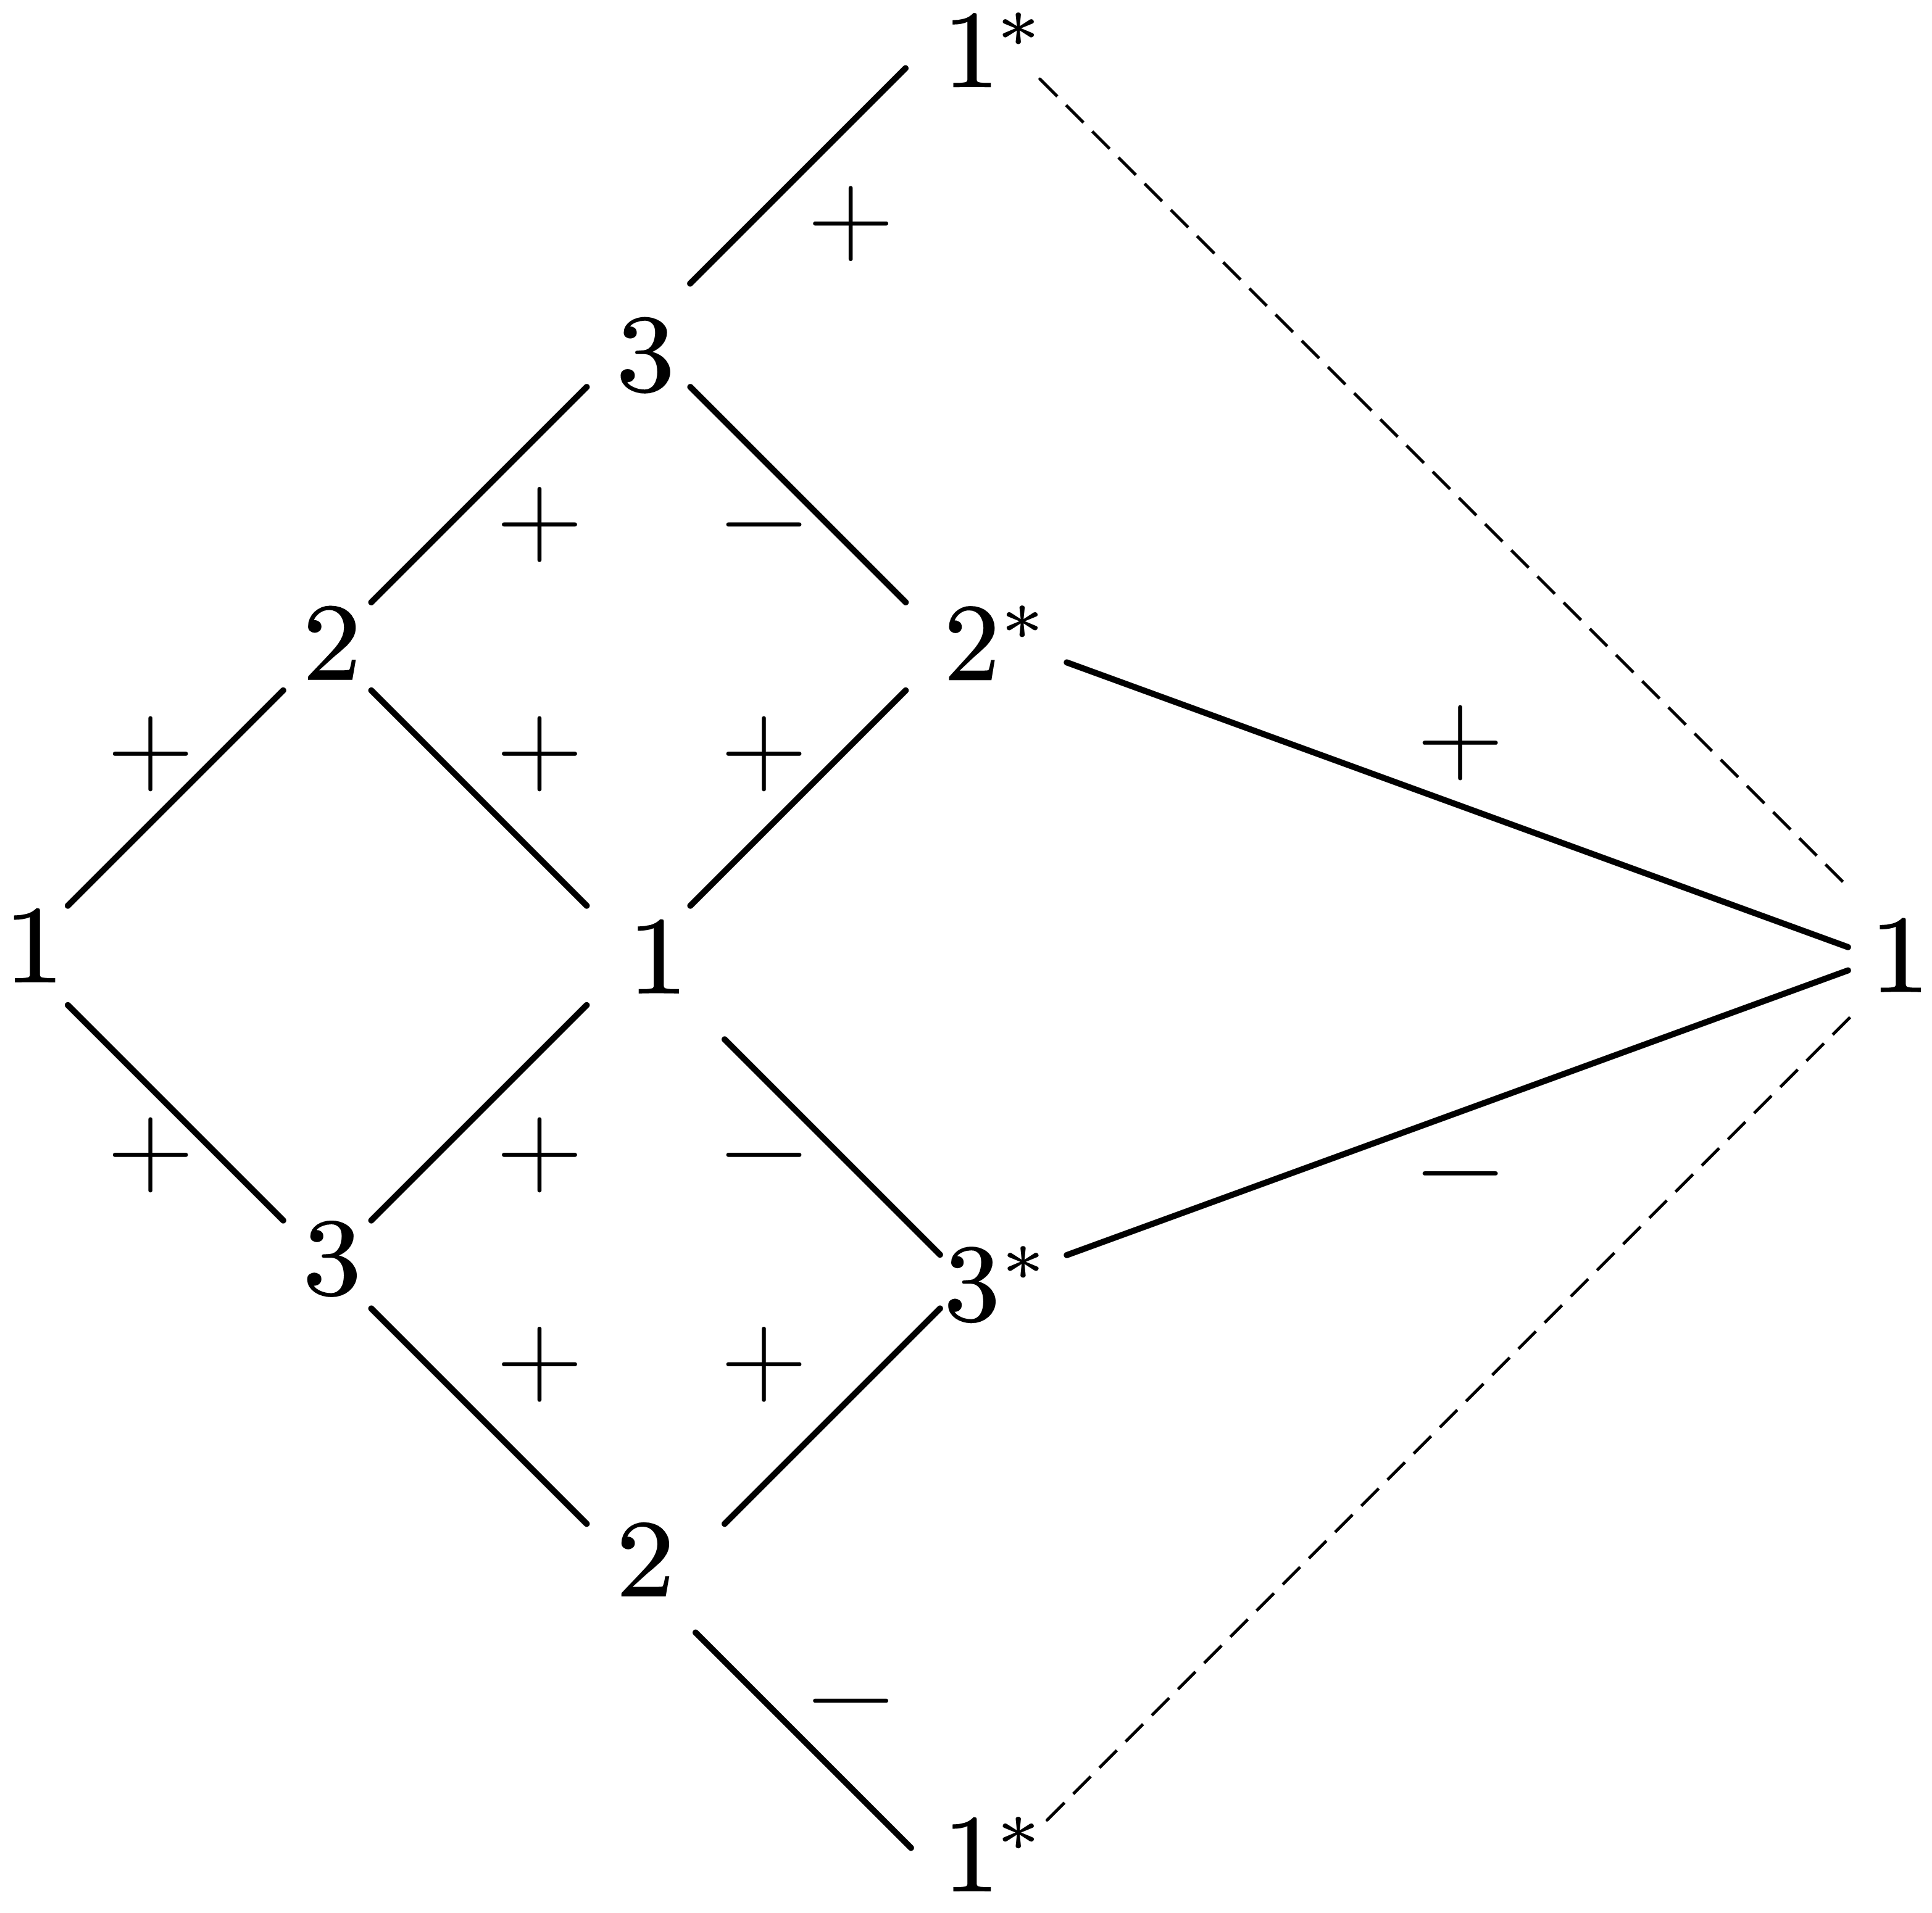
\includegraphics[scale=0.5,trim=0 -8 0 -8]{./pictures/6.07/pictorial_representation_2.png}
		\end{minipage} &
		
		\begin{minipage}{0.3\linewidth}
		\centering
		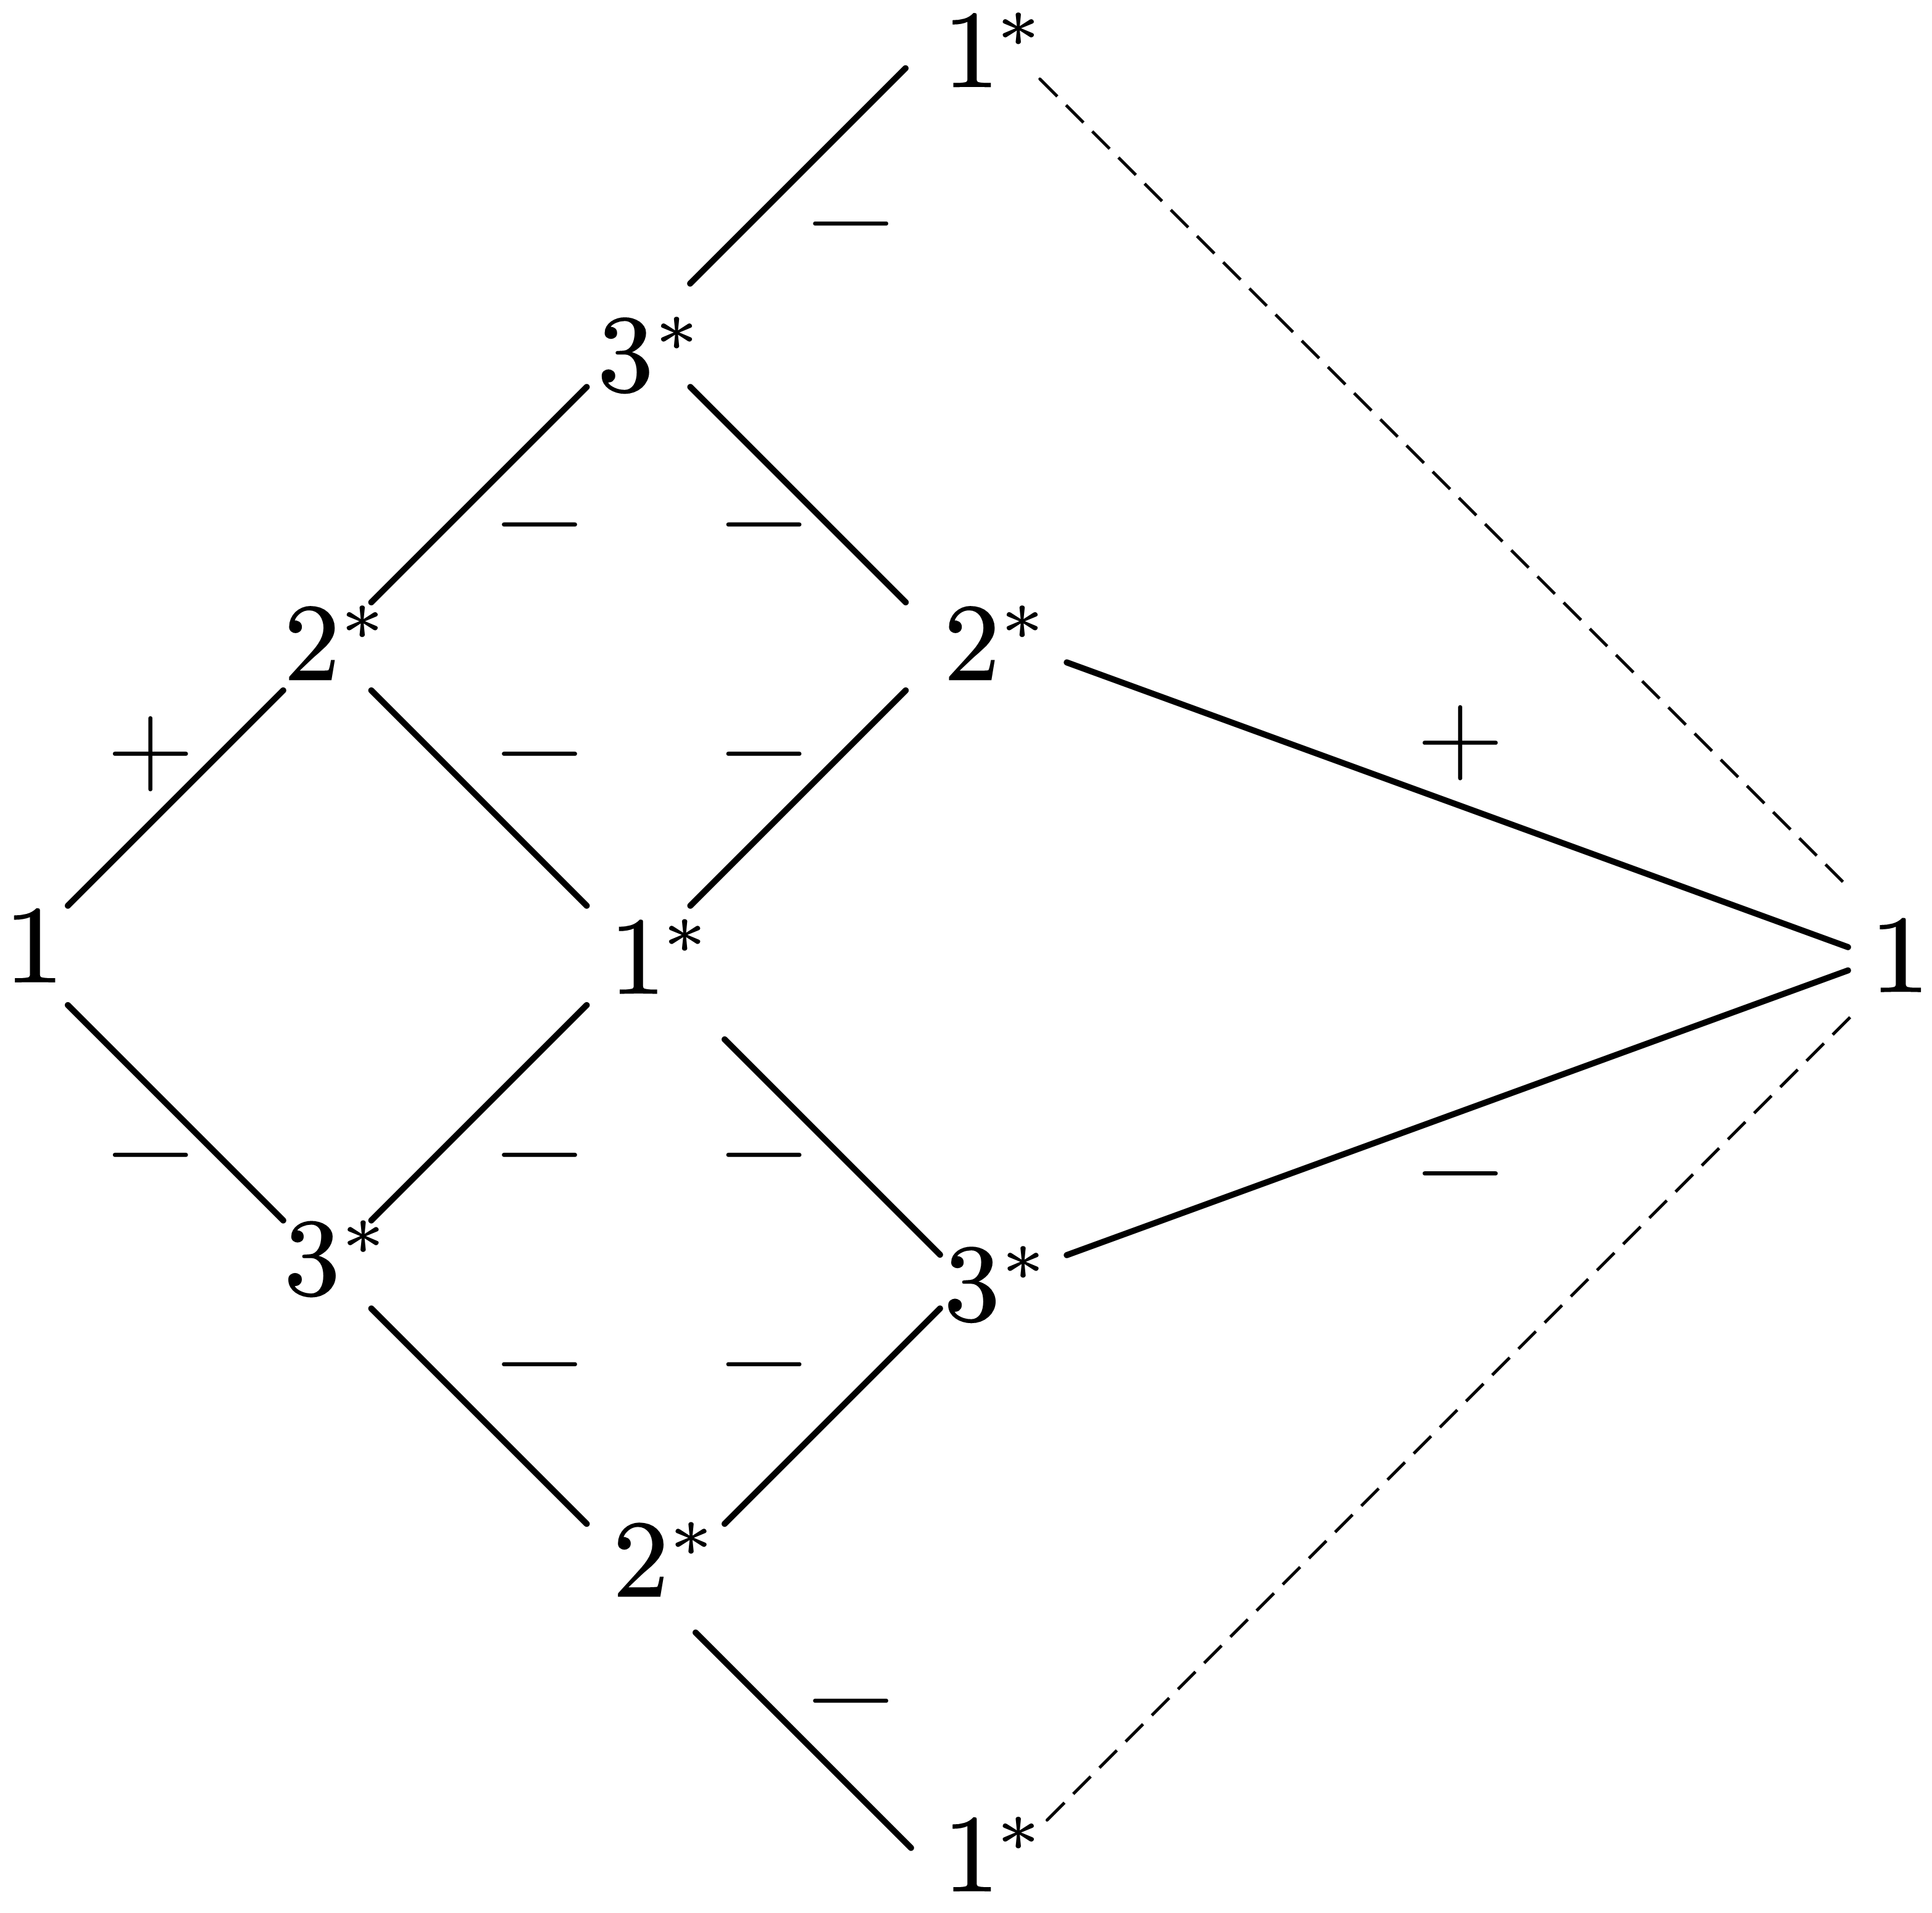
\includegraphics[scale=0.5,trim=0 -8 0 -8]{./pictures/6.07/pictorial_representation_3.png}
		\end{minipage} \\
		
		\begin{minipage}{0.3\linewidth}
		\centering
		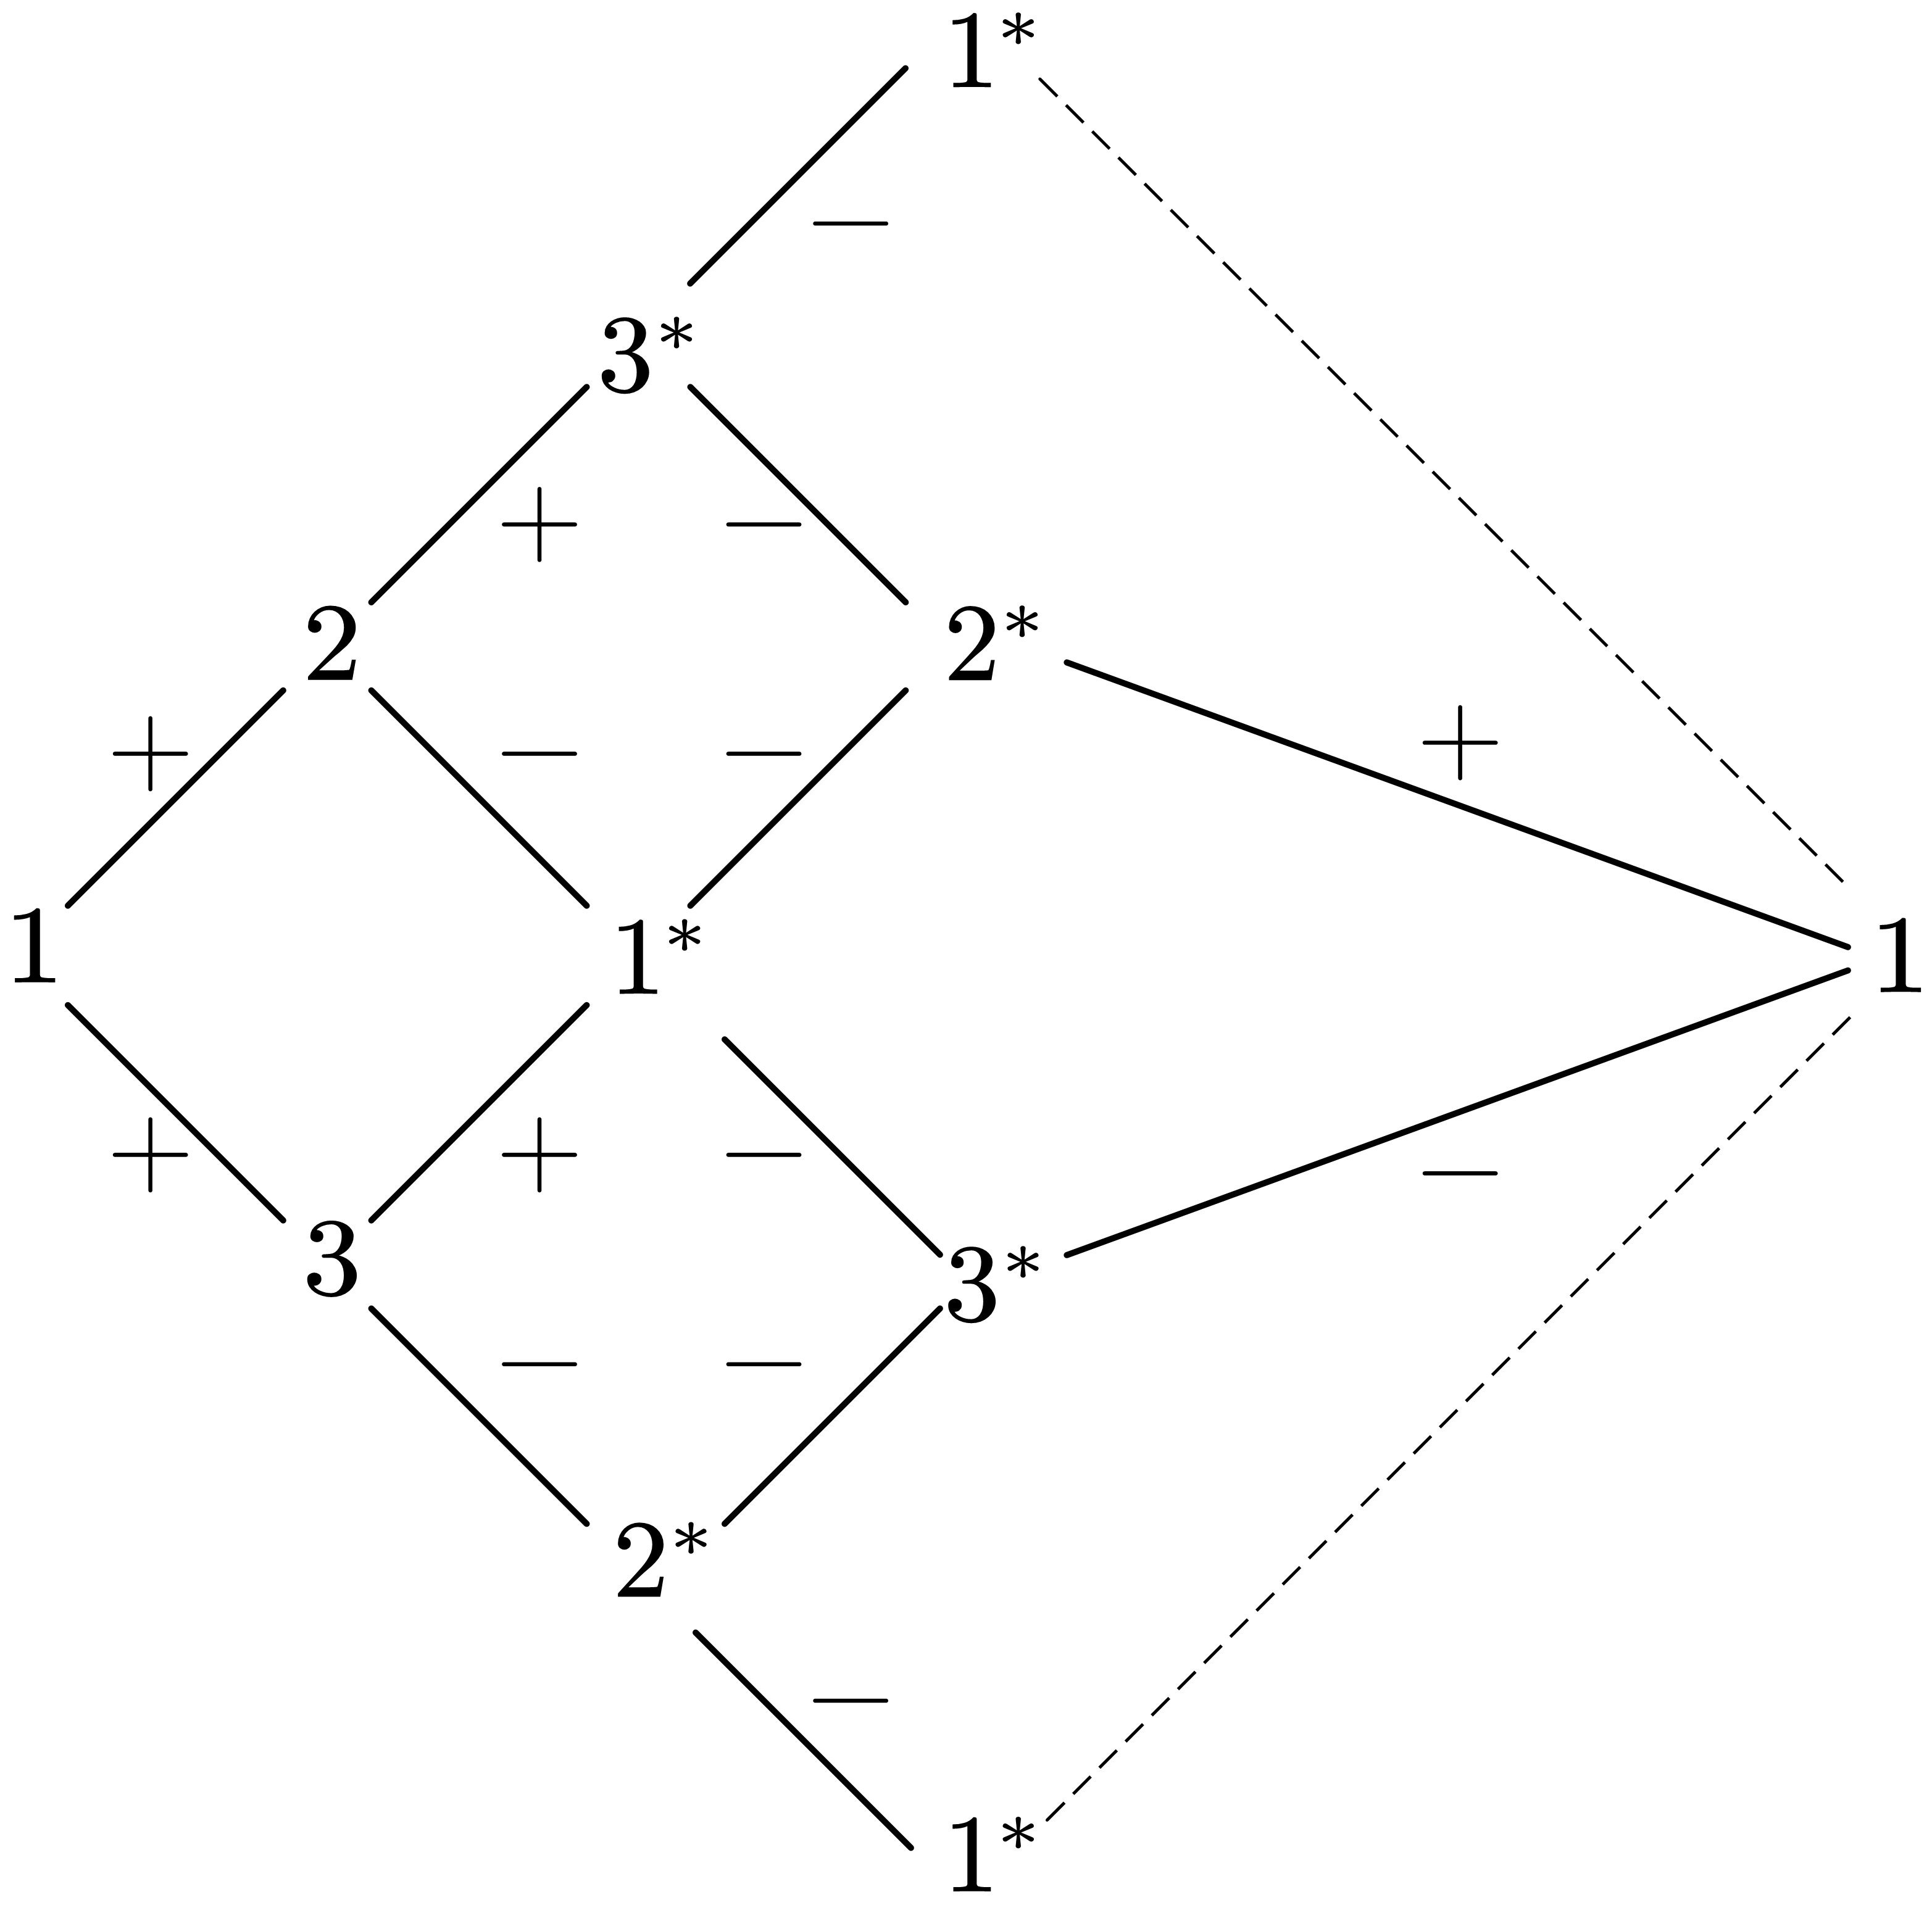
\includegraphics[scale=0.5,trim=0 -8 0 -8]{./pictures/6.07/pictorial_representation_4.png}
		\end{minipage} &
			
		\begin{minipage}{0.3\linewidth}
		\centering
		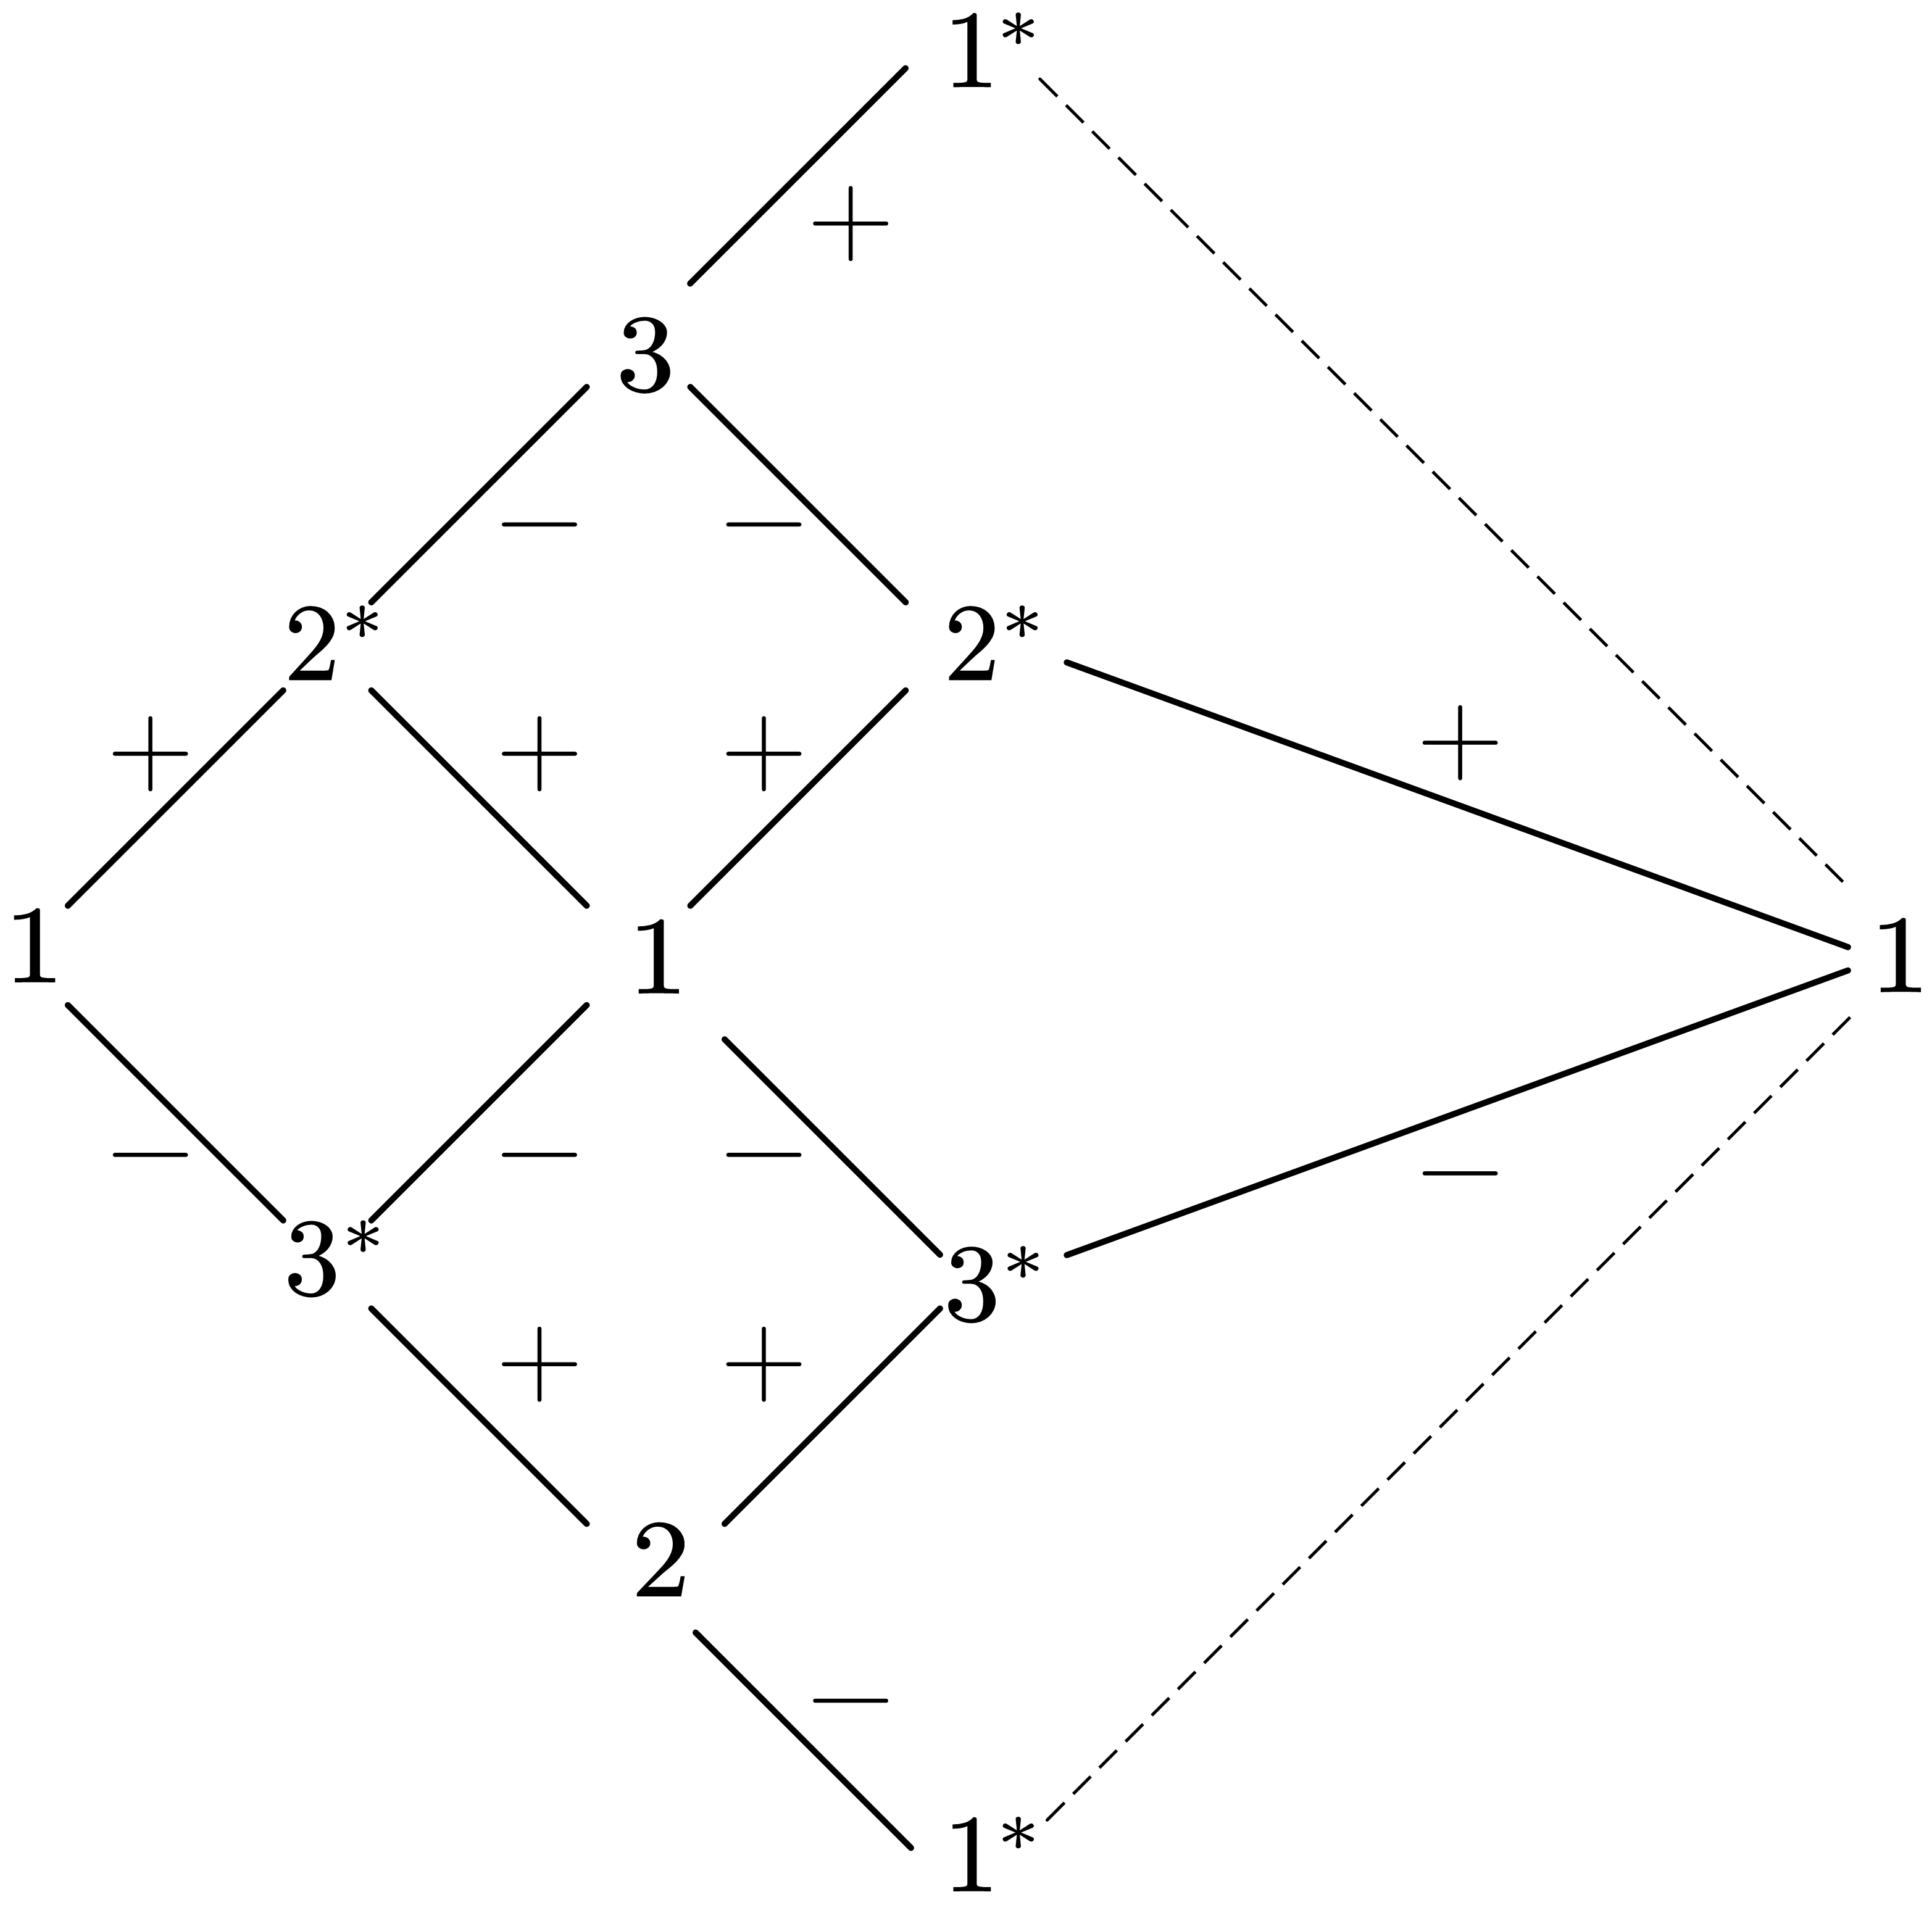
\includegraphics[scale=0.5,trim=0 -8 0 -8]{./pictures/6.07/pictorial_representation_5.png}
		\end{minipage} &
		
		\begin{minipage}{0.3\linewidth}
		\centering
		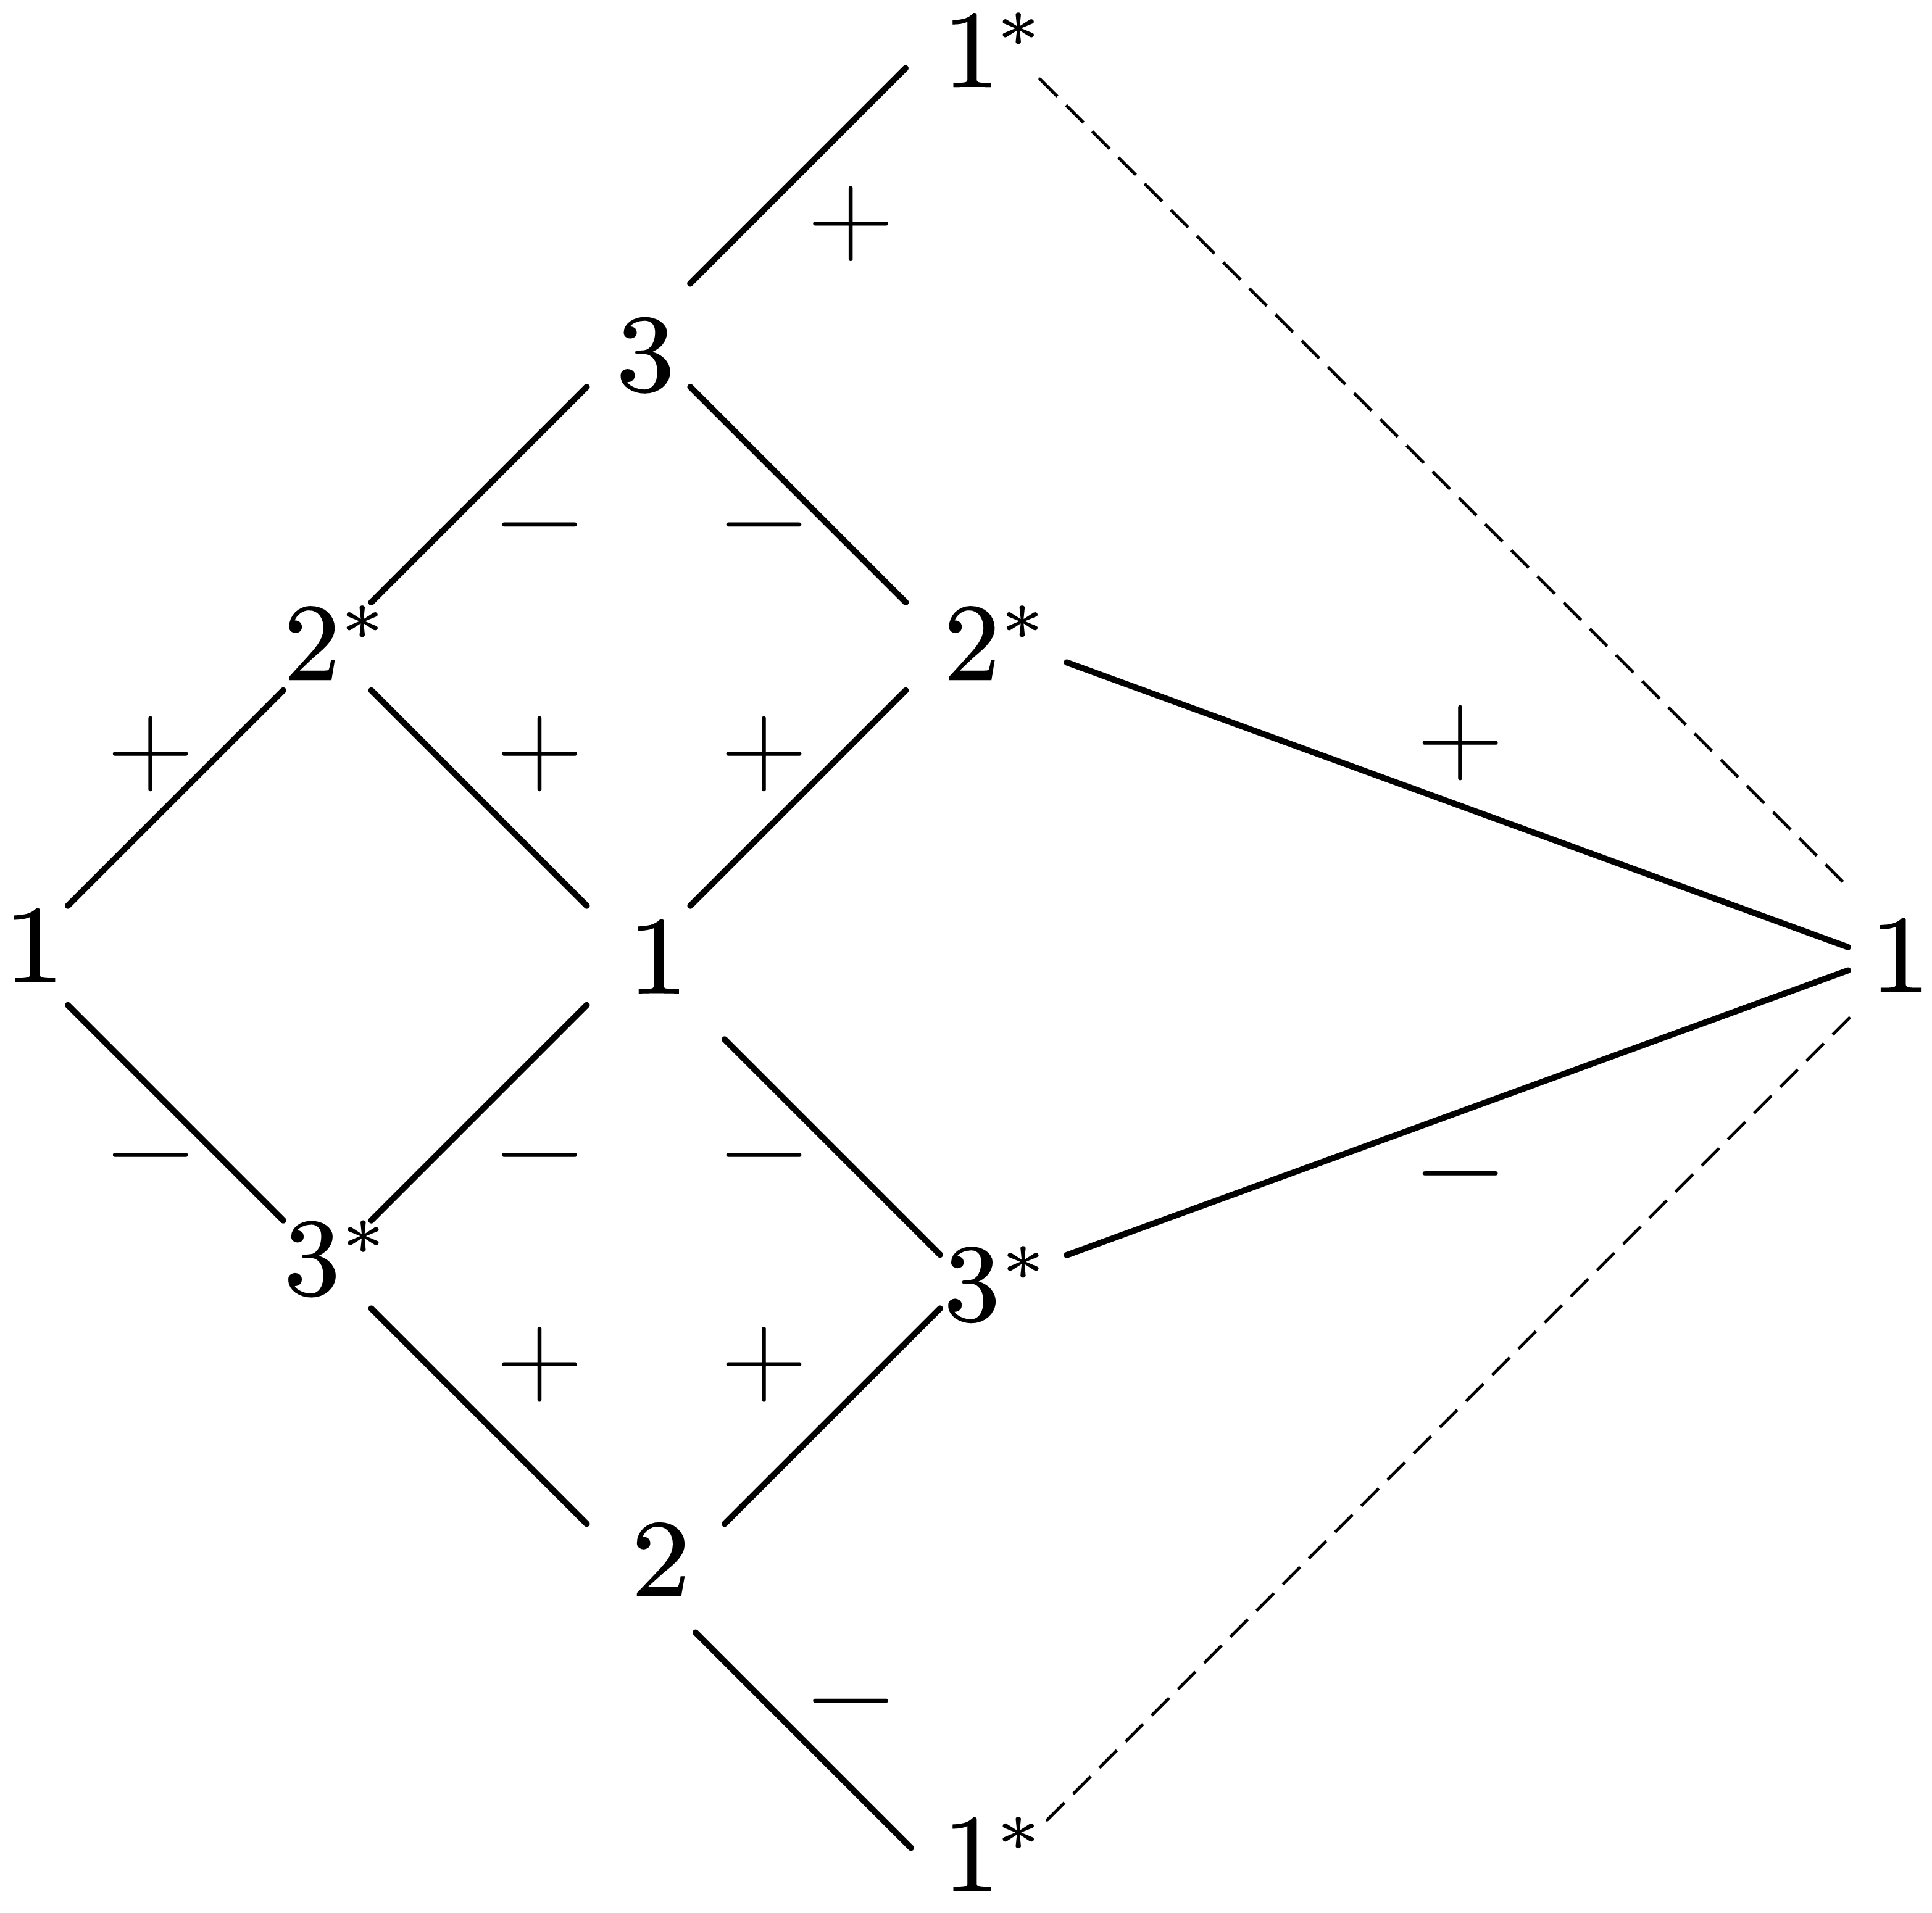
\includegraphics[scale=0.5,trim=0 -8 0 -8]{./pictures/6.07/pictorial_representation_6.png}
		\end{minipage}
		
	\end{tabular}
	\captionof{figure}{The pictorial representation of all fourth-order diagrams of the benzene.}\label{fig:exe7_2}
	\end{center}
	
	Now we will calculate all terms according to their pictorial representation. Instead of lengthy calculation, we only care about the path from 1 to 1 in each diagram. For example, for the first subdiagram of \Figref{fig:exe7_2}, we know that it has eight paths, six valid but two invalid. If a path has a segment with a plus/minus token, it will be marked as $+$/$-$, and zero otherwise. And thus, its eight paths are:
	\begin{center}
	\begin{tabular}{cccc}
		$(+,+,-,0)$ & $(+,+,-,+)$ & $(+,-,-,+)$ & $(+,-,-,-)$\\
		$(+,+,-,+)$ & $(+,+,-,-)$ & $(+,-,-,-)$ & $(+,-,-,0)$
	\end{tabular}
	\end{center}		
	If a path has a 0, the corresponding term is zero. Otherwise, the corresponding term has a factor $(-1)^k$, where $k$ is the number of its minus signs. Therefore, there are two positive and four negative terms, and the first term is
	\[
		(-1)^{2+1} \frac{2 \times 3}{ (2\beta)^3 } \left[ 2 \times \left( \frac{\beta^4}{16} \right) + 4 \times \left( -\frac{\beta^4}{16} \right) \right] = \frac{6}{64} \beta = \frac{N}{64} \beta,
	\]
	where the factor $2$ occurs for the closed-shell structure, and the factor $3$ is the number of occupied spin orbitals.
	
	Similarly, we find that the second, third, ..., sixth term is $\frac{N}{64} \beta$, $\frac{N}{64} \beta$, $\frac{N}{64} \beta$, $-\frac{3N}{128} \beta$, $-\frac{3N}{128} \beta$. Thus, we obtain that
	\begin{sequation}
		E^{(4)}_0 = 4 \times \left( \frac{N}{64} \beta \right) + 2 \times \left( -\frac{3N}{128} \beta \right) = \frac{N}{64} \beta.
	\end{sequation}

	\item[b.] As mentioned before, the general expression of the correlation energy with $N>6$ is also suitable for benzene. Thus, the correlation energy of the benzene is
	\begin{sequation}
		E^{(4)}_0({\rm benzene} ) = \frac{6}{64} \beta = \frac{3}{32} \beta,
	\end{sequation}		
	which agrees with the independently calculated result found in Exercise 6.6.
	
	\end{itemize}	
	
	\end{solution}
	
	\section{Perturbation Expansion of the Correlation Energy}
	
	% 6.8
	\begin{exercise}
	Derive Eqs.(6.73) and (6.74) starting with Eq.(6.72).
	\end{exercise}
	
	\begin{solution}

	The detailed simplification can be seen in Exercise 2.18.
	
	\end{solution}
	
	% 6.9
	\begin{exercise}
	Derive Eqs.(6.77) and (6.78) from Eq.(6.76).
	\end{exercise}
	
	\begin{solution}
	We assume that $\Delta \approx (\varepsilon_2 - \varepsilon_1)$, thus	
	\[
		\Delta = ( \varepsilon_2 - \varepsilon_1 ) + \frac{1}{2} J_{11} + \frac{1}{2} J_{22} - 2 J_{12} + K_{12} = ( \varepsilon_2 - \varepsilon_1 ) \left[ 1 + \frac{ J_{11} + J_{22} - 4 J_{12} + 2 K_{12} }{ 2 ( \varepsilon_2 - \varepsilon_1 ) } \right].
	\]
	Using binomial series and geometric series, we find that
	\begin{align*}
		E_\corr &= \Delta - \left( \Delta^2 + K^2_{12} \right)^{\frac{1}{2}} = \Delta \left[ 1 - \left( 1 + \frac{ K^2_{12} }{ \Delta^2 } \right)^{\frac{1}{2}} \right] = \Delta \left[ 1 - \left( 1 + \frac{ K^2_{12} }{ 2\Delta^2 } - \frac{ K^4_{12} }{ 8\Delta^4 } + \cdots \right) \right] \\
		&= - \frac{ K^2_{12} }{ 2\Delta } + \frac{ K^4_{12} }{ 8\Delta^3 } + \cdots \\
		&= - \frac{ K^2_{12} }{ 2( \varepsilon_2 - \varepsilon_1 ) \left[ 1 + \frac{ J_{11} + J_{22} - 4 J_{12} + 2 K_{12} }{ 2 ( \varepsilon_2 - \varepsilon_1 ) } \right] } + \frac{ K^4_{12} }{ 8 ( \varepsilon_2 - \varepsilon_1 )^3 \left[ 1 + \frac{ J_{11} + J_{22} - 4 J_{12} + 2 K_{12} }{ 2 ( \varepsilon_2 - \varepsilon_1 ) } \right]^3 } + \cdots \\
		&= - \frac{ K^2_{12} }{ 2( \varepsilon_2 - \varepsilon_1 )} \left[ 1 - \frac{ J_{11} + J_{22} - 4 J_{12} + 2 K_{12} }{ 2 ( \varepsilon_2 - \varepsilon_1 ) } + \left( \frac{ J_{11} + J_{22} - 4 J_{12} + 2 K_{12} }{ 2 ( \varepsilon_2 - \varepsilon_1 ) } \right)^2 + \cdots \right] + \cdots \\
		&= - \frac{ K^2_{12} }{ 2( \varepsilon_2 - \varepsilon_1 )} + \frac{ K^2_{12} ( J_{11} + J_{22} - 4 J_{12} + 2 K_{12} ) }{ 4( \varepsilon_2 - \varepsilon_1 )^2 } + o\left( \left( \frac{1}{ \varepsilon_2 - \varepsilon_1 } \right)^2 \right) .
	\end{align*}
	Thus, we obtain (6.77) and (6.78) from (6.76).
	
	\end{solution}
	
	\section{The \texorpdfstring{$N$}--Dependence of the RS Perturbation Expansion}
	
	% 6.10
	\begin{exercise}
	Derive Eqs.(6.80b) and (6.90).
	\end{exercise}
	
	\begin{solution}
	From (6.68), we find that with the truth that all two-electron integrals involving orbitals from different units are zero and $\langle mm || mm \rangle = 0$,
	\begin{align*}
		E^{(1)}_0 &= - \frac{1}{2} \sum_{ i=1 }^{2N} \sum_{ j=1 }^{2N} \langle 1_i 1_j || 1_i 1_j \rangle = - \frac{1}{2} \sum_{ i=1 }^{2N} \langle 1_i 1_i || 1_i 1_i \rangle \\
			&= - \frac{1}{2} \sum_{ i=1 }^N \langle 1_i 1_i || 1_i 1_i \rangle + \langle 1_i \bar{1}_i || 1_i \bar{1}_i \rangle + \langle \bar{1}_i 1_i || \bar{1}_i 1_i \rangle + \langle \bar{1}_i \bar{1}_i || \bar{1}_i \bar{1}_i \rangle = -\frac{1}{2} \sum_{ i=1 }^N 2J_{11} = -\sum_{ i=1 }^N J_{11} = -N J_{11}.
	\end{align*}
	
	Besides, we obtain that
	\begin{align*}
		\langle \Psi^{2_i \bar{2}_i}_{1_i \bar{1}_i} | \mathscr{V} | \Psi^{2_i \bar{2}_i}_{1_i \bar{1}_i} \rangle &= \langle \Psi^{2_i \bar{2}_i}_{1_i \bar{1}_i} | \mathscr{H} | \Psi^{2_i \bar{2}_i}_{1_i \bar{1}_i} \rangle - \langle \Psi^{2_i \bar{2}_i}_{1_i \bar{1}_i} | \mathscr{H}_0 | \Psi^{2_i \bar{2}_i}_{1_i \bar{1}_i} \rangle \\
		&= \sum_{ i=1 }^{2N} h_{11} + 2h_{22} - 2h_{11} + \sum_{ i=1 }^N  J_{11} + J_{22} - J_{11} - \left[ ( 2N - 2 ) \varepsilon_1 + 2\varepsilon_2 \right] \\
		&= (2N-2)h_{11} + 2h_{22} + (N-1) J_{11} + J_{22} - (2N-2) ( h_{11} + J_{11} ) - 2 (h_{22} + 2J_{12} - K_{12})\\
		&= -(N-1) J_{11} + J_{22} - 4J_{12} + 2K_{12}. 
	\end{align*}
	
	\end{solution}
	
	\sectionstar{Diagrammatic Representation of the Perturbation Expansion of the Correlation Energy}
	
	\subsection{Hugenholtz Diagrams}
	
	% 6.11
	\begin{exercise}
	Show that the fourth-order diagram
	
	\begin{center}
	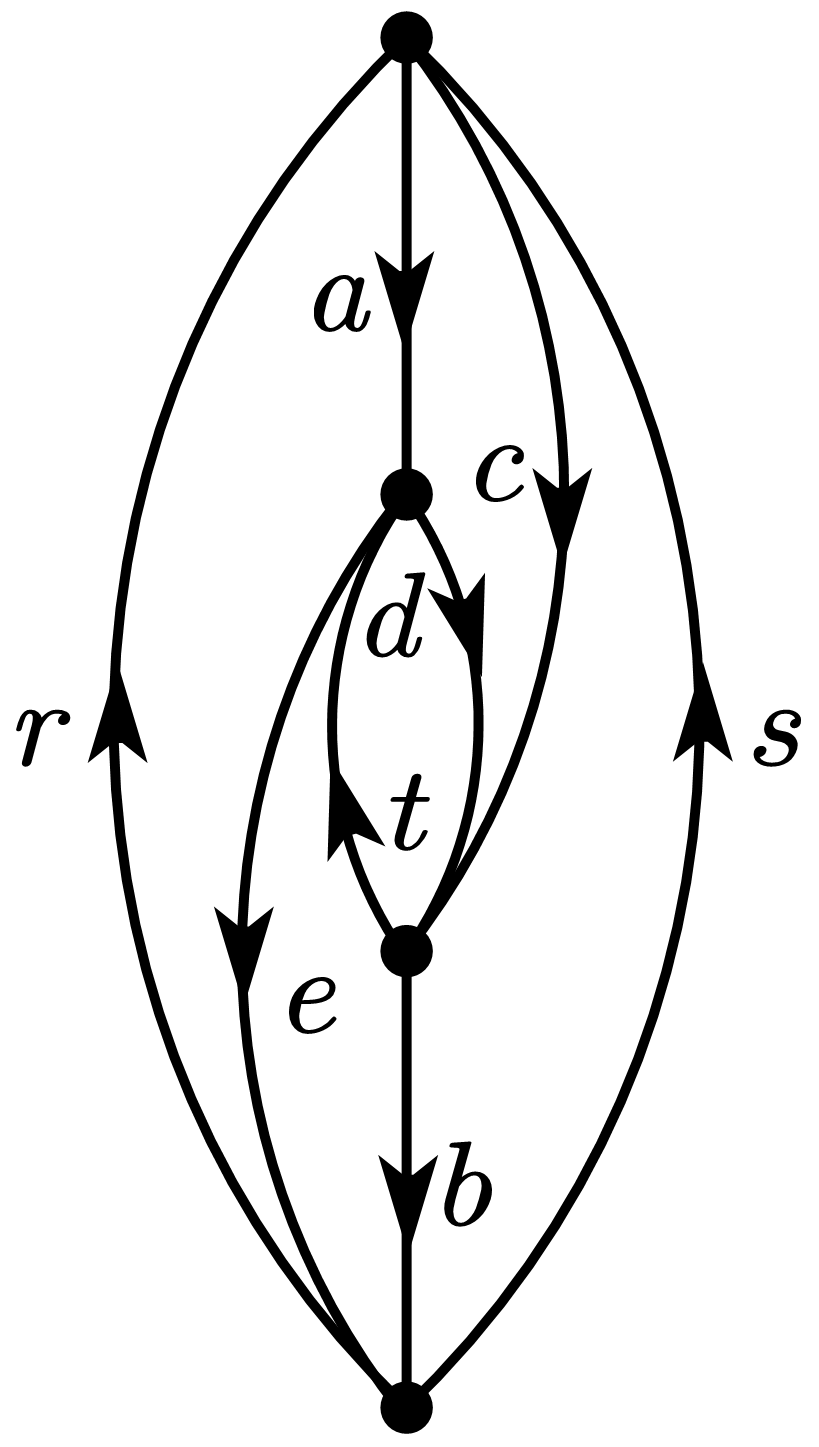
\includegraphics[scale=0.9]{./pictures/6.11/exercise.png}
	\end{center}
	is equal to
	\[
		-\frac{1}{2} \sum_{abcderst} \frac{ \langle rs || ac \rangle \langle at || de \rangle \langle dc || tb \rangle \langle eb||rs \rangle }{ ( \varepsilon_a + \varepsilon_c - \varepsilon_r - \varepsilon_s ) ( \varepsilon_c + \varepsilon_d + \varepsilon_e - \varepsilon_r - \varepsilon_t - \varepsilon_s ) ( \varepsilon_b + \varepsilon_e - \varepsilon_r - \varepsilon_s ) }.
	\]	
	
	\end{exercise}
	
	\begin{solution}
	
	Using the diagrammatic method, this term is made of four parts as follows.
	\begin{enumerate}
	
	\item There are 5 hole lines ($a$, $b$, $c$, $d$, $e$) and 3 particle lines ($r$, $s$, $t$). Thus we add a summation token with subscripts $abcderst$. 
	
	\item There are 2 loops, $r \rightarrow a \rightarrow d \rightarrow t \rightarrow e \rightarrow r$, $s \rightarrow c \rightarrow b \rightarrow s$, and 5 hole lines, thus we should add a $(-1)^{2+5} = (-1)^7$.	
	
	\item From the top to the bottom, 4 dots contribute $\langle rs|| ac \rangle$, $\langle at||de \rangle$, $\langle dc || tb \rangle$, $\langle eb || rs \rangle$, respectively.
	
	\item There are 3 imaginary horizontal lines.
		\begin{itemize}
		
		\item The first one crosses $a$, $c$, $r$, $s$, contributing a factor $\varepsilon_a + \varepsilon_c - \varepsilon_r - \varepsilon_s$ to the denominator.
		
		\item The second one crosses $c$, $d$, $e$, $r$, $t$, $s$ contributing a factor $\varepsilon_c + \varepsilon_d + \varepsilon_e - \varepsilon_r - \varepsilon_t - \varepsilon_s$ to the denominator.
		
		\item The third one crosses $b$, $e$, $r$, $s$, contributing a factor $\varepsilon_b + \varepsilon_e - \varepsilon_r - \varepsilon_s$ to the denominator.
		
		\end{itemize}			
	
	\end{enumerate}
	
	In conclusion, we know the mathematical expression of this diagram is
	\begin{sequation}
		-\frac{1}{2} \sum_{abcderst} \frac{ \langle rs || ac \rangle \langle at || de \rangle \langle dc || tb \rangle \langle eb||rs \rangle }{ ( \varepsilon_a + \varepsilon_c - \varepsilon_r - \varepsilon_s ) ( \varepsilon_c + \varepsilon_d + \varepsilon_e - \varepsilon_r - \varepsilon_t - \varepsilon_s ) ( \varepsilon_b + \varepsilon_e - \varepsilon_r - \varepsilon_s ) }.
	\end{sequation}
	
	\end{solution}
	
	\subsection{Goldstone Diagrams}
	
	% 6.12
	\begin{exercise}
	We stated that the Goldstone diagrams in Table 6.2 can be obtained by ``pulling apart" the second- and third-order Hugenholtz diagrams. This is quite tricky to see but the converse is much easier. For example, if we push
	
	\begin{center}
	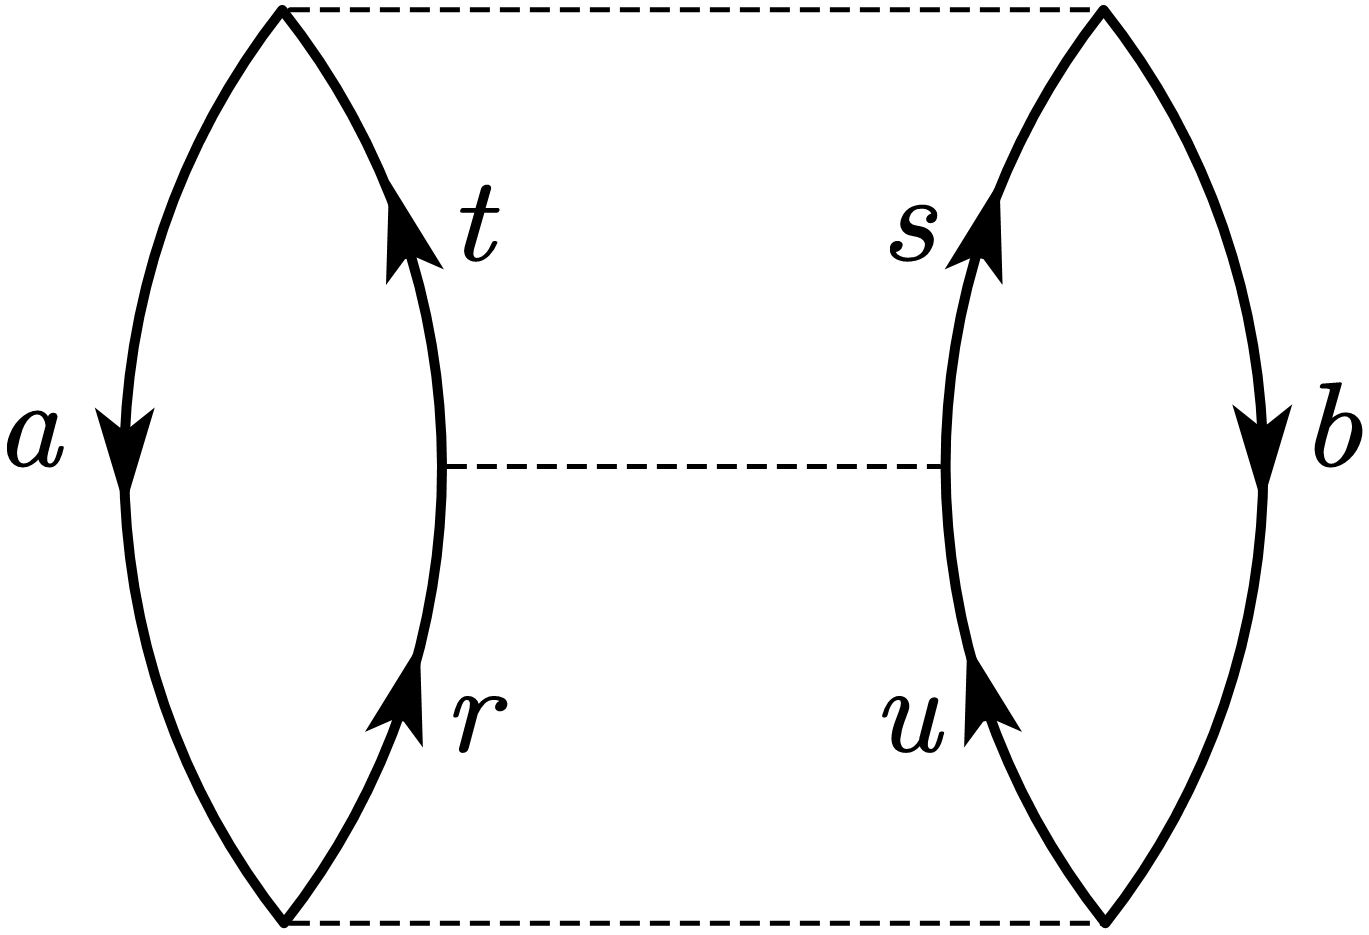
\includegraphics[scale=0.9]{./pictures/6.12/exercise_1.png}
	\end{center}
	
	together, it is clear that we obtain
	
	\begin{center}
	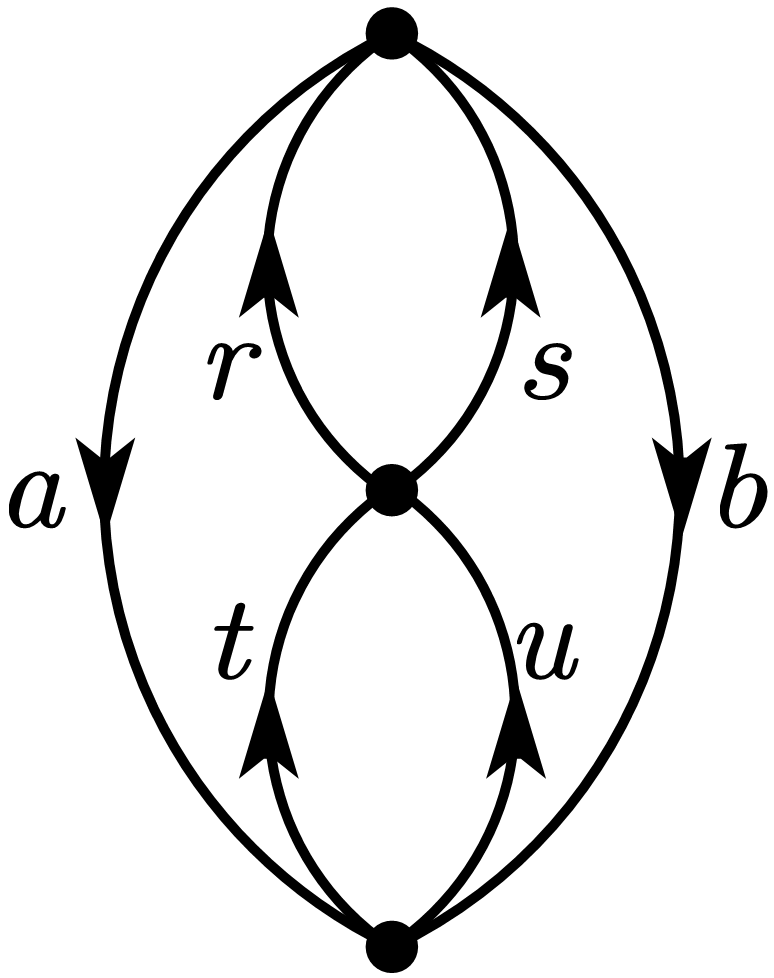
\includegraphics[scale=0.9]{./pictures/6.12/exercise_2.png}
	\end{center}
	
	Push all third-order diagrams in Table 6.2 together in a similar way and, thus, find which Goldstone diagram comes from which Hugenholtz diagram. For the above Hugenholtz diagram, verify that its mathematical value is indeed the sum of the values of the corresponding Goldstone diagrams.
	
	\end{exercise}
	
	\begin{solution}

	As the textbook mentioned at the page 361, there are three third-order Hugenholtz diagrams, which are listed in \Figref{fig:exe12_1}.

	\begin{center}
	\begin{tabular}{ccc}
	
		\begin{minipage}{0.22\linewidth}
		\centering
		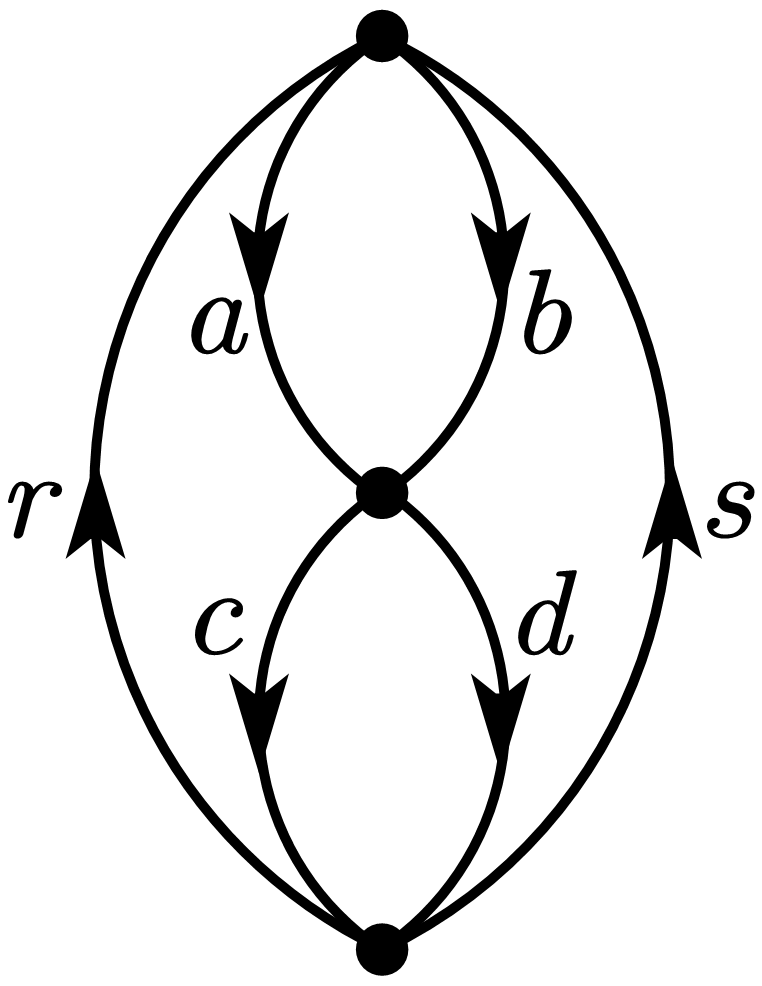
\includegraphics[scale=1.0,trim=0 -4 0 -4]{./pictures/6.12/hugenholtz_1.png}
		\end{minipage} &
		
		\begin{minipage}{0.22\linewidth}
		\centering
		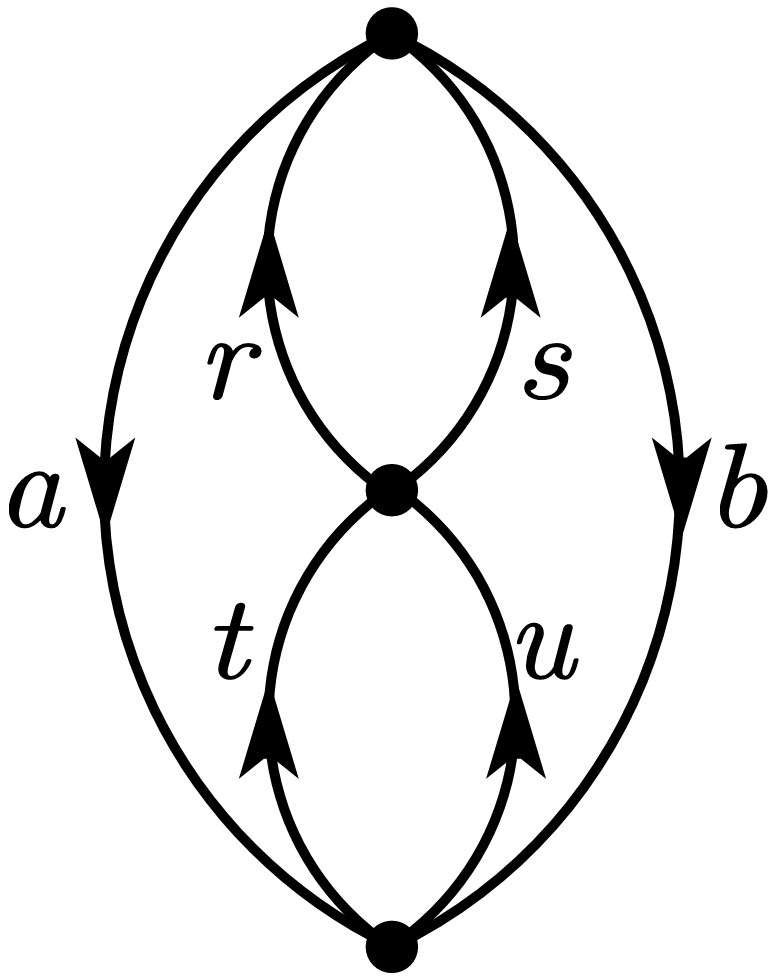
\includegraphics[scale=1.0,trim=0 -4 0 -4]{./pictures/6.12/hugenholtz_2.png}
		\end{minipage} &
		
		\begin{minipage}{0.22\linewidth}
		\centering
		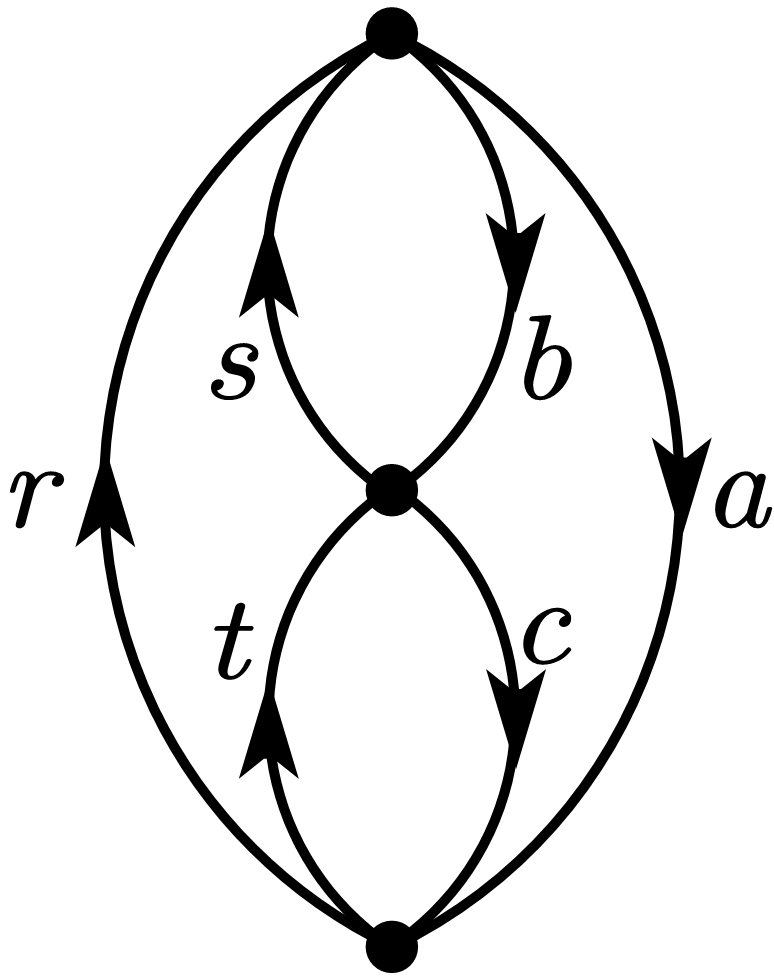
\includegraphics[scale=1.0,trim=0 -4 0 -4]{./pictures/6.12/hugenholtz_3.png}
		\end{minipage}
		
	\end{tabular}
	\captionof{figure}{All third-order Hugenholtz diagrams.}\label{fig:exe12_1}
	\end{center}
	
	In fact, the ``pushing together" results of these third-order Goldstone diagrams in the table 6.2 can be summarized as follows.
	\begin{itemize}
	
	\item Pushing together the second or the seventh third-order Goldstone diagrams leads to the first Hugenholtz diagram.
	
	\item Pushing together the first and the eighth third-order Goldstone diagrams leads to the second Hugenholtz diagram.
	
	\item Pushing together the rest of third-order Goldstone diagrams leads to the third Hugenholtz diagram.
	
	\end{itemize}
	
	Firstly, we will verify that the sum of the second and the seventh third-order Goldstone diagrams is the first third-order Hugenholtz diagram. The sum of the second and the seventh third-order Goldstone diagrams is
	\begin{align*}
		&\hspace{1.4em} (-1)^{4+2} \left( \frac{1}{2} \right) \sum_{abcdrs} \frac{ \langle ad | rs \rangle \langle cb | ad \rangle \langle rs | cb \rangle }{ ( \varepsilon_a + \varepsilon_d - \varepsilon_r - \varepsilon_s ) ( \varepsilon_c + \varepsilon_b - \varepsilon_r - \varepsilon_s ) } \\
		&\hspace{6em} + (-1)^{4+1} \left( \frac{1}{2} \right) \sum_{abcdrs} \frac{ \langle ac | rs \rangle \langle db | ac \rangle \langle sr | db \rangle }{ ( \varepsilon_a + \varepsilon_c - \varepsilon_r - \varepsilon_s ) ( \varepsilon_d + \varepsilon_b - \varepsilon_r - \varepsilon_s ) } \\
		&= \frac{1}{2} \sum_{abcdrs} \frac{ \langle ad | rs \rangle \langle cb | ad \rangle \langle rs | cb \rangle }{ ( \varepsilon_a + \varepsilon_d - \varepsilon_r - \varepsilon_s ) ( \varepsilon_c + \varepsilon_b - \varepsilon_r - \varepsilon_s ) } - \frac{ \langle ad | rs \rangle \langle cb | ad \rangle \langle sr | cb \rangle }{ ( \varepsilon_a + \varepsilon_d - \varepsilon_r - \varepsilon_s ) ( \varepsilon_c + \varepsilon_b - \varepsilon_r - \varepsilon_s ) } \\
		&= \frac{1}{2} \sum_{abcdrs} \frac{ \langle ad | rs \rangle \langle cb | ad \rangle \left( \langle rs | cb \rangle - \langle sr | cb \rangle \right) }{ ( \varepsilon_a + \varepsilon_d - \varepsilon_r - \varepsilon_s ) ( \varepsilon_c + \varepsilon_b - \varepsilon_r - \varepsilon_s ) } = \frac{1}{2} \sum_{abcdrs} \frac{ \langle ab | rs \rangle \langle cd | ab \rangle \left( \langle rs | cd \rangle - \langle sr | cd \rangle \right) }{ ( \varepsilon_a + \varepsilon_b - \varepsilon_r - \varepsilon_s ) ( \varepsilon_c + \varepsilon_d - \varepsilon_r - \varepsilon_s ) },
	\end{align*}
	and the first Hugenholtz diagram can be simplified to
	\begin{align*}
		&\hspace{1.4em} \frac{1}{8} \sum_{abcdrs} \frac{ \langle ab || rs \rangle \langle rs || cd \rangle \langle cd || ab \rangle }{ ( \varepsilon_a + \varepsilon_b - \varepsilon_r - \varepsilon_s ) ( \varepsilon_c + \varepsilon_d - \varepsilon_r - \varepsilon_s ) } \\
		&= \frac{1}{8} \sum_{abcdrs} \frac{ ( \langle ab | rs \rangle - \langle ab | sr \rangle )( \langle rs | cd \rangle - \langle rs | dc \rangle ) ( \langle cd | ab \rangle - \langle cd | ba \rangle ) }{ ( \varepsilon_a + \varepsilon_b - \varepsilon_r - \varepsilon_s ) ( \varepsilon_c + \varepsilon_d - \varepsilon_r - \varepsilon_s ) } \\
		&= \frac{1}{8} \sum_{abcdrs} \frac{ \langle ab | rs \rangle \langle rs | cd \rangle \langle cd | ab \rangle }{ ( \varepsilon_a + \varepsilon_b - \varepsilon_r - \varepsilon_s ) ( \varepsilon_c + \varepsilon_d - \varepsilon_r - \varepsilon_s ) } - \frac{ \langle ab | rs \rangle \langle rs | cd \rangle \langle cd | ba \rangle }{ ( \varepsilon_a + \varepsilon_b - \varepsilon_r - \varepsilon_s ) ( \varepsilon_c + \varepsilon_d - \varepsilon_r - \varepsilon_s ) } \\
		&\hspace{6em} - \frac{ \langle ab | rs \rangle \langle rs | dc \rangle \langle cd | ab \rangle }{ ( \varepsilon_a + \varepsilon_b - \varepsilon_r - \varepsilon_s ) ( \varepsilon_c + \varepsilon_d - \varepsilon_r - \varepsilon_s ) } + \frac{ \langle ab | rs \rangle \langle rs | dc \rangle \langle cd | ba \rangle }{ ( \varepsilon_a + \varepsilon_b - \varepsilon_r - \varepsilon_s ) ( \varepsilon_c + \varepsilon_d - \varepsilon_r - \varepsilon_s ) } \\
		&\hspace{6em} - \frac{ \langle ab | sr \rangle \langle rs | cd \rangle \langle cd | ab \rangle }{ ( \varepsilon_a + \varepsilon_b - \varepsilon_r - \varepsilon_s ) ( \varepsilon_c + \varepsilon_d - \varepsilon_r - \varepsilon_s ) } + \frac{ \langle ab | sr \rangle \langle rs | cd \rangle \langle cd | ba \rangle }{ ( \varepsilon_a + \varepsilon_b - \varepsilon_r - \varepsilon_s ) ( \varepsilon_c + \varepsilon_d - \varepsilon_r - \varepsilon_s ) } \\
		&\hspace{6em} + \frac{ \langle ab | sr \rangle \langle rs | dc \rangle \langle cd | ab \rangle }{ ( \varepsilon_a + \varepsilon_b - \varepsilon_r - \varepsilon_s ) ( \varepsilon_c + \varepsilon_d - \varepsilon_r - \varepsilon_s ) } - \frac{ \langle ab | sr \rangle \langle rs | dc \rangle \langle cd | ba \rangle }{ ( \varepsilon_a + \varepsilon_b - \varepsilon_r - \varepsilon_s ) ( \varepsilon_c + \varepsilon_d - \varepsilon_r - \varepsilon_s ) } \\
		&= \frac{1}{8} \sum_{abcdrs} \frac{ \langle ab | rs \rangle \langle cd | ab \rangle \langle rs | cd \rangle }{ ( \varepsilon_a + \varepsilon_b - \varepsilon_r - \varepsilon_s ) ( \varepsilon_c + \varepsilon_d - \varepsilon_r - \varepsilon_s ) } - \frac{ \langle ab | rs \rangle \langle rs | dc \rangle \langle dc | ba \rangle }{ ( \varepsilon_a + \varepsilon_b - \varepsilon_r - \varepsilon_s ) ( \varepsilon_c + \varepsilon_d - \varepsilon_r - \varepsilon_s ) } \\
		&\hspace{6em} - \frac{ \langle ab | rs \rangle \langle sr | cd \rangle \langle cd | ab \rangle }{ ( \varepsilon_a + \varepsilon_b - \varepsilon_r - \varepsilon_s ) ( \varepsilon_c + \varepsilon_d - \varepsilon_r - \varepsilon_s ) } + \frac{ \langle ab | rs \rangle \langle sr | dc \rangle \langle dc | ba \rangle }{ ( \varepsilon_a + \varepsilon_b - \varepsilon_r - \varepsilon_s ) ( \varepsilon_c + \varepsilon_d - \varepsilon_r - \varepsilon_s ) } \\
		&\hspace{6em} - \frac{ \langle ab | rs \rangle \langle sr | cd \rangle \langle cd | ab \rangle }{ ( \varepsilon_a + \varepsilon_b - \varepsilon_r - \varepsilon_s ) ( \varepsilon_c + \varepsilon_d - \varepsilon_r - \varepsilon_s ) } + \frac{ \langle ab | rs \rangle \langle sr | dc \rangle \langle dc | ba \rangle }{ ( \varepsilon_a + \varepsilon_b - \varepsilon_r - \varepsilon_s ) ( \varepsilon_c + \varepsilon_d - \varepsilon_r - \varepsilon_s ) } \\
		&\hspace{6em} + \frac{ \langle ab | rs \rangle \langle sr | dc \rangle \langle cd | ab \rangle }{ ( \varepsilon_a + \varepsilon_b - \varepsilon_r - \varepsilon_s ) ( \varepsilon_c + \varepsilon_d - \varepsilon_r - \varepsilon_s ) } - \frac{ \langle ab | rs \rangle \langle sr | cd \rangle \langle dc | ba \rangle }{ ( \varepsilon_a + \varepsilon_b - \varepsilon_r - \varepsilon_s ) ( \varepsilon_c + \varepsilon_d - \varepsilon_r - \varepsilon_s ) } \\
		&= \frac{1}{2} \sum_{abcdrs} \frac{ \langle ab | rs \rangle \langle cd | ab \rangle \left( \langle rs | cd \rangle - \langle sr | cd \rangle \right) }{ ( \varepsilon_a + \varepsilon_b - \varepsilon_r - \varepsilon_s ) ( \varepsilon_c + \varepsilon_d - \varepsilon_r - \varepsilon_s ) }.
	\end{align*}
	Thus, we have verified that the sum of the second and the seventh third-order Goldstone diagrams is the first third-order Hugenholtz diagram.
	
	Secondly, we will verify that the sum of the first and the eighth third-order Goldstone diagrams is the second third-order Hugenholtz diagram. The sum of the first and the eighth third-order Goldstone diagrams is
	\begin{align*}
		&(-1)^{2+2} \left( \frac{1}{2} \right) \sum_{abrsut} \frac{ \langle ab | ru \rangle \langle ru | ts \rangle \langle ts | ab \rangle }{ ( \varepsilon_a + \varepsilon_b - \varepsilon_r - \varepsilon_u ) ( \varepsilon_a + \varepsilon_b - \varepsilon_t - \varepsilon_s ) } \\
		&\hspace{6em}+ (-1)^{2+1} \left( \frac{1}{2} \right) \sum_{abrsut} \frac{ \langle ab | rt \rangle \langle tr | us \rangle \langle us | ab \rangle }{ ( \varepsilon_a + \varepsilon_b - \varepsilon_t - \varepsilon_r ) ( \varepsilon_a + \varepsilon_b - \varepsilon_u - \varepsilon_s ) } \\
		&= \frac{1}{2} \sum_{abrsut} \frac{ \langle ab | ru \rangle \langle ru | ts \rangle \langle ts | ab \rangle }{ ( \varepsilon_a + \varepsilon_b - \varepsilon_r - \varepsilon_u ) ( \varepsilon_a + \varepsilon_b - \varepsilon_t - \varepsilon_s ) } - \frac{ \langle ab | ru \rangle \langle ur | ts \rangle \langle ts | ab \rangle }{ ( \varepsilon_a + \varepsilon_b - \varepsilon_u - \varepsilon_r ) ( \varepsilon_a + \varepsilon_b - \varepsilon_t - \varepsilon_s ) } \\
		&= \frac{1}{2} \sum_{abrsut} \frac{ \langle ab | ru \rangle \langle ts | ab \rangle ( \langle ru | ts \rangle - \langle ur | ts \rangle ) }{ ( \varepsilon_a + \varepsilon_b - \varepsilon_r - \varepsilon_u ) ( \varepsilon_a + \varepsilon_b - \varepsilon_t - \varepsilon_s ) } = \frac{1}{2} \sum_{abrsut} \frac{ \langle ab | rs \rangle \langle tu | ab \rangle ( \langle rs | tu \rangle - \langle sr | tu \rangle ) }{ ( \varepsilon_a + \varepsilon_b - \varepsilon_r - \varepsilon_s ) ( \varepsilon_a + \varepsilon_b - \varepsilon_t - \varepsilon_u ) }.
	\end{align*}
	and the second Hugenholtz diagram can be simplified to
	\begin{align*}
		&\hspace{1.4em} \frac{1}{8} \sum_{abrstu} \frac{ \langle ab || rs \rangle \langle rs || tu \rangle \langle tu || ab \rangle }{ ( \varepsilon_a + \varepsilon_b - \varepsilon_r - \varepsilon_s ) ( \varepsilon_a + \varepsilon_b - \varepsilon_t - \varepsilon_u ) } \\
		&= \frac{1}{8} \sum_{abrstu} \frac{ ( \langle ab | rs \rangle - \langle ab | sr \rangle )( \langle rs | tu \rangle - \langle rs | ut \rangle ) ( \langle tu | ab \rangle - \langle tu | ba \rangle ) }{ ( \varepsilon_a + \varepsilon_b - \varepsilon_r - \varepsilon_s ) ( \varepsilon_a + \varepsilon_b - \varepsilon_t - \varepsilon_u ) } \\
		&= \frac{1}{8} \sum_{abrstu} \frac{ \langle ab | rs \rangle \langle rs | tu \rangle \langle tu | ab \rangle }{ ( \varepsilon_a + \varepsilon_b - \varepsilon_r - \varepsilon_s ) ( \varepsilon_a + \varepsilon_b - \varepsilon_t - \varepsilon_u ) } - \frac{ \langle ab | rs \rangle \langle rs | tu \rangle \langle tu | ba \rangle }{ ( \varepsilon_a + \varepsilon_b - \varepsilon_r - \varepsilon_s ) ( \varepsilon_a + \varepsilon_b - \varepsilon_t - \varepsilon_u ) } \\
		&\hspace{6em} - \frac{ \langle ab | rs \rangle \langle rs | ut \rangle \langle tu | ab \rangle }{ ( \varepsilon_a + \varepsilon_b - \varepsilon_r - \varepsilon_s ) ( \varepsilon_a + \varepsilon_b - \varepsilon_t - \varepsilon_u ) } + \frac{ \langle ab | rs \rangle \langle rs | ut \rangle \langle tu | ba \rangle }{ ( \varepsilon_a + \varepsilon_b - \varepsilon_r - \varepsilon_s ) ( \varepsilon_a + \varepsilon_b - \varepsilon_t - \varepsilon_u ) } \\
		&\hspace{6em} - \frac{ \langle ab | sr \rangle \langle rs | tu \rangle \langle tu | ab \rangle }{ ( \varepsilon_a + \varepsilon_b - \varepsilon_r - \varepsilon_s ) ( \varepsilon_a + \varepsilon_b - \varepsilon_t - \varepsilon_u ) } + \frac{ \langle ab | sr \rangle \langle rs | tu \rangle \langle tu | ba \rangle }{ ( \varepsilon_a + \varepsilon_b - \varepsilon_r - \varepsilon_s ) ( \varepsilon_a + \varepsilon_b - \varepsilon_t - \varepsilon_u ) } \\
		&\hspace{6em} + \frac{ \langle ab | sr \rangle \langle rs | ut \rangle \langle tu | ab \rangle }{ ( \varepsilon_a + \varepsilon_b - \varepsilon_r - \varepsilon_s ) ( \varepsilon_a + \varepsilon_b - \varepsilon_t - \varepsilon_u ) } - \frac{ \langle ab | sr \rangle \langle rs | ut \rangle \langle tu | ba \rangle }{ ( \varepsilon_a + \varepsilon_b - \varepsilon_r - \varepsilon_s ) ( \varepsilon_a + \varepsilon_b - \varepsilon_t - \varepsilon_u ) } \\
		&= \frac{1}{8} \sum_{abrstu} \frac{ \langle ab | rs \rangle \langle rs | tu \rangle \langle tu | ab \rangle }{ ( \varepsilon_a + \varepsilon_b - \varepsilon_r - \varepsilon_s ) ( \varepsilon_a + \varepsilon_b - \varepsilon_t - \varepsilon_u ) } - \frac{ \langle ab | rs \rangle \langle rs | ut \rangle \langle ut | ba \rangle }{ ( \varepsilon_a + \varepsilon_b - \varepsilon_r - \varepsilon_s ) ( \varepsilon_a + \varepsilon_b - \varepsilon_t - \varepsilon_u ) } \\
		&\hspace{6em} - \frac{ \langle ab | rs \rangle \langle rs | tu \rangle \langle ut | ab \rangle }{ ( \varepsilon_a + \varepsilon_b - \varepsilon_r - \varepsilon_s ) ( \varepsilon_a + \varepsilon_b - \varepsilon_t - \varepsilon_u ) } + \frac{ \langle ab | rs \rangle \langle rs | tu \rangle \langle ut | ba \rangle }{ ( \varepsilon_a + \varepsilon_b - \varepsilon_r - \varepsilon_s ) ( \varepsilon_a + \varepsilon_b - \varepsilon_t - \varepsilon_u ) } \\
		&\hspace{6em} - \frac{ \langle ab | rs \rangle \langle sr | tu \rangle \langle tu | ab \rangle }{ ( \varepsilon_a + \varepsilon_b - \varepsilon_r - \varepsilon_s ) ( \varepsilon_a + \varepsilon_b - \varepsilon_t - \varepsilon_u ) } + \frac{ \langle ab | rs \rangle \langle sr | ut \rangle \langle ut | ba \rangle }{ ( \varepsilon_a + \varepsilon_b - \varepsilon_r - \varepsilon_s ) ( \varepsilon_a + \varepsilon_b - \varepsilon_t - \varepsilon_u ) } \\
		&\hspace{6em} + \frac{ \langle ab | rs \rangle \langle sr | ut \rangle \langle tu | ab \rangle }{ ( \varepsilon_a + \varepsilon_b - \varepsilon_r - \varepsilon_s ) ( \varepsilon_a + \varepsilon_b - \varepsilon_t - \varepsilon_u ) } - \frac{ \langle ab | rs \rangle \langle sr | tu \rangle \langle ut | ba \rangle }{ ( \varepsilon_a + \varepsilon_b - \varepsilon_r - \varepsilon_s ) ( \varepsilon_a + \varepsilon_b - \varepsilon_t - \varepsilon_u ) } \\
		&= \frac{1}{2} \sum_{abrstu} \frac{ \langle ab | rs \rangle \langle rs | tu \rangle \langle tu | ab \rangle }{ ( \varepsilon_a + \varepsilon_b - \varepsilon_r - \varepsilon_s ) ( \varepsilon_a + \varepsilon_b - \varepsilon_t - \varepsilon_u ) } - \frac{ \langle ab | rs \rangle \langle rs | ut \rangle \langle ut | ba \rangle }{ ( \varepsilon_a + \varepsilon_b - \varepsilon_r - \varepsilon_s ) ( \varepsilon_a + \varepsilon_b - \varepsilon_t - \varepsilon_u ) } \\
		&= \frac{1}{2} \sum_{abrsut} \frac{ \langle ab | rs \rangle \langle tu | ab \rangle ( \langle rs | tu \rangle - \langle sr | tu \rangle ) }{ ( \varepsilon_a + \varepsilon_b - \varepsilon_r - \varepsilon_s ) ( \varepsilon_a + \varepsilon_b - \varepsilon_t - \varepsilon_u ) }.
	\end{align*}
	Thus, we have verified that the sum of the first and the eighth third-order Goldstone diagrams is the second third-order Hugenholtz diagram.
	
	Thirdly, we will verify that the sum of the rest of third-order Goldstone diagrams is the third third-order Hugenholtz diagram. The third third-order Hugenholtz diagram is	
	\begin{align*}
		&\hspace{1.4em}\sum_{abcrst} \frac{ \langle ab || rs \rangle \langle cs || tb \rangle \langle rt || ac \rangle }{ ( \varepsilon_a + \varepsilon_b - \varepsilon_s - \varepsilon_r ) ( \varepsilon_a + \varepsilon_c - \varepsilon_r - \varepsilon_t ) } \\
		&= \sum_{abcrst} \frac{ [ \langle ab | rs \rangle - \langle ab | sr \rangle ] [ \langle cs | tb \rangle - \langle cs | bt \rangle ] [ \langle rt | ac \rangle - \langle rt | ca \rangle ] }{ ( \varepsilon_a + \varepsilon_b - \varepsilon_s - \varepsilon_r ) ( \varepsilon_a + \varepsilon_c - \varepsilon_r - \varepsilon_t ) } \\
		&= \sum_{abcrst} \frac{ \langle ab | rs \rangle \langle cs | tb \rangle \langle rt | ac \rangle }{ ( \varepsilon_a + \varepsilon_b - \varepsilon_r - \varepsilon_s ) ( \varepsilon_a + \varepsilon_c - \varepsilon_r - \varepsilon_t ) } - \frac{ \langle ab | rs \rangle \langle cs | tb \rangle \langle rt | ca \rangle }{ ( \varepsilon_a + \varepsilon_b - \varepsilon_r - \varepsilon_s ) ( \varepsilon_a + \varepsilon_c - \varepsilon_r - \varepsilon_t ) } \\
		&\hspace{4em} - \frac{ \langle ab | rs \rangle \langle cs | bt \rangle \langle rt | ac \rangle }{ ( \varepsilon_a + \varepsilon_b - \varepsilon_r - \varepsilon_s ) ( \varepsilon_a + \varepsilon_c - \varepsilon_r - \varepsilon_t ) } + \frac{ \langle ab | rs \rangle \langle cs | bt \rangle \langle rt | ca \rangle }{ ( \varepsilon_a + \varepsilon_b - \varepsilon_r - \varepsilon_s ) ( \varepsilon_a + \varepsilon_c - \varepsilon_r - \varepsilon_t ) } \\
		&\hspace{4em} - \frac{ \langle ab | sr \rangle \langle cs | tb \rangle \langle rt | ac \rangle }{ ( \varepsilon_a + \varepsilon_b - \varepsilon_r - \varepsilon_s ) ( \varepsilon_a + \varepsilon_c - \varepsilon_r - \varepsilon_t ) } + \frac{ \langle ab | sr \rangle \langle cs | tb \rangle \langle rt | ca \rangle }{ ( \varepsilon_a + \varepsilon_b - \varepsilon_r - \varepsilon_s ) ( \varepsilon_a + \varepsilon_c - \varepsilon_r - \varepsilon_t ) } \\
		&\hspace{4em} + \frac{ \langle ab | sr \rangle \langle cs | bt \rangle \langle rt | ac \rangle }{ ( \varepsilon_a + \varepsilon_b - \varepsilon_r - \varepsilon_s ) ( \varepsilon_a + \varepsilon_c - \varepsilon_r - \varepsilon_t ) } - \frac{ \langle ab | sr \rangle \langle cs | bt \rangle \langle rt | ca \rangle }{ ( \varepsilon_a + \varepsilon_b - \varepsilon_r - \varepsilon_s ) ( \varepsilon_a + \varepsilon_c - \varepsilon_r - \varepsilon_t ) } \\
		&= \sum_{abcrst} \frac{ \langle ac | rt \rangle \langle bt | sc \rangle \langle rs | ab \rangle }{ ( \varepsilon_a + \varepsilon_c - \varepsilon_r - \varepsilon_t ) ( \varepsilon_a + \varepsilon_b - \varepsilon_r - \varepsilon_s ) } - \frac{ \langle bc | rt \rangle \langle at | sc \rangle \langle rs | ab \rangle }{ ( \varepsilon_b + \varepsilon_c - \varepsilon_t - \varepsilon_r ) ( \varepsilon_a + \varepsilon_b - \varepsilon_r - \varepsilon_s ) } \\
		&\hspace{2em} - \sum_{abcrst} \frac{ \langle bc | rt \rangle \langle ra | sb \rangle \langle st | ac \rangle }{ ( \varepsilon_b + \varepsilon_c - \varepsilon_r - \varepsilon_t ) ( \varepsilon_a + \varepsilon_c - \varepsilon_s - \varepsilon_t ) } + \sum_{abcrst} \frac{ \langle bc | rt \rangle \langle ar | bs \rangle \langle ts | ac \rangle }{ ( \varepsilon_c + \varepsilon_b - \varepsilon_r - \varepsilon_t ) ( \varepsilon_a + \varepsilon_c - \varepsilon_s - \varepsilon_t ) } \\
		&\hspace{2em} - \sum_{abcrst} \frac{ \langle ab | rs \rangle \langle sc | at \rangle \langle rt | bc \rangle }{ ( \varepsilon_a + \varepsilon_b - \varepsilon_r - \varepsilon_s ) ( \varepsilon_c + \varepsilon_b - \varepsilon_r - \varepsilon_t ) } + \sum_{abcrst} \frac{ \langle cb | rt \rangle \langle at | sc \rangle \langle rs | ab \rangle }{ ( \varepsilon_c + \varepsilon_b - \varepsilon_r - \varepsilon_t ) ( \varepsilon_a + \varepsilon_b - \varepsilon_r - \varepsilon_s ) } \\
		&\hspace{2em} + \sum_{abcrst} \frac{ \langle cb | rt \rangle \langle ra | sb \rangle \langle st | ac \rangle }{ ( \varepsilon_c + \varepsilon_b - \varepsilon_r - \varepsilon_t ) ( \varepsilon_a + \varepsilon_c - \varepsilon_s - \varepsilon_t ) } - \sum_{abcrst} \frac{ \langle ac | rt \rangle \langle rb | sc \rangle \langle st | ab \rangle }{ ( \varepsilon_a + \varepsilon_c - \varepsilon_r - \varepsilon_t ) ( \varepsilon_a + \varepsilon_b - \varepsilon_s - \varepsilon_t ) }.
	\end{align*}	
	These eight terms correspond to the fifth, twelfth, fourth, ninth, eleventh, sixth, tenth, third third-order Goldstone diagrams, respectively.
	
	In conclusion, we have verified that the first third-order Hugenholtz diagram corresponds the second and the seventh third-order Goldstone diagrams, the second third-order Hugenholtz diagram corresponds the first and the eighth third-order Goldstone diagrams, and the third third-order Hugenholtz diagram corresponds the third, fourth, fifth, sixth, ninth, tenth, eleventh, twelfth third-order Goldstone diagrams.
	\end{solution}
	
	\subsection{Summation of Diagrams}
	
	\subsection{What Is the Linked Cluster Theorem?}
	
	% 6.13
	\begin{exercise}
	Calculate $E^{(3)}_0$ for a supermolecule consisting of $N$ non-interacting minimal basis $\ce{H2}$ molecules by evaluating the Goldstone diagrams in Table 6.2. Compare your result with that of Eq.(6.92), which was obtained algebraically by explicitly cancelling terms proportional to $N^2$.
	
	{\it Hint}: Simply show that the value of each Goldstone diagram for the supermolecule in $N$ times the result for a single molecule.
	\end{exercise}
	
	\begin{solution}
	Note that in this model, all two-electron integrals involving orbitals from different units are zero, and all third-order terms in the table 6.2 will be zero unless their numerators are non-zero. Thus, each third-order term of this model is just the sum of that of each units, leading that the value of each Goldstone diagram for the supermolecule in $N$ times the result for a single molecule.
	\end{solution}
	
	\section{Some Illustrative Calculations}

\end{document}
